\section{Varietà topologiche e differenziabili}

\subsection{Spazi topologici}

Una topologia $ \tau $ su un insieme non vuoto $ X $ è una classe non vuota di sottoinsiemi di $ X $, i.e. $ \tau \subset \ps(X) $ (dove $ \ps(X) $ indica l'insieme delle parti di $ X $), per la quale valgono:

\begin{enumerate}
	\item $ \emptyset, X \in \tau $
	
	\item L'unione di un numero qualsiasi di insiemi di $ \tau $ appartiene a $ \tau $
	
	\item L'intersezione di due insiemi qualsiasi di $ \tau $ appartiene a $ \tau $
\end{enumerate}

La coppia $ (X, \tau) $ è detta \textit{spazio topologico}; in queste note, indicheremo con $ X $ lo spazio topologico $ (X, \tau) $, sottintendendo la topologia $ \tau $ quando questa è chiara dal contesto.

\subsection{Varietà topologiche}

Sia $ X $ uno spazio topologico, diremo che $ X $ è una \textit{varietà topologica} se sono soddisfatte le seguenti condizioni:

\begin{itemize}
	\item $ X $ è $ T_{2} $ o \textit{di Hausdorff}, i.e. dati due punti distinti di $ X $ è sempre possibile trovare due intorni disgiunti che contengano i due punti
	
	\item $ X $ è $ N_{2} $ o \textit{a base numerabile}, i.e. esiste una base per la topologia di $ X $ che sia numerabile\footnote{%
		Un insieme è numerabile se possiede la stessa cardinalità dell'insieme dei numeri naturali $ \N $; in notazione, $ \# \mathfrak{B} = \# \N = \aleph_{0} $.}
	
	\item $ X $ è \textit{localmente euclideo}, i.e. 
		\begin{equation}
			\forall p \in X, \, \E \text{aperto } U \ni p \wedge \E \phi : U \to \R^{n} \, \mid \, \phi : U \to \phi(U) \subset \R^{n} \text{ omeomorfismo}
		\end{equation}
		dunque localmente ogni aperto di $ X $ è omeomorfo a un aperto di $ \R^{n} $
\end{itemize}

La coppia $ (U,\phi) $ è chiamata \textit{carta intorno a} $ p $; se $ \phi(p) = 0 $, la carta è detta \textit{centrata} in $ p $.\\
Diremo che, se lo spazio topologico è localmente omeomorfo a $ \R^{n} $, la sua dimensione è pari a quella di quest'ultimo, i.e. $ \dim (X) = n $.

\sbs{0.55}{%
			\begin{remark}
				Possiamo sempre assumere che $ \phi(U) \equiv \R^{n} $. Questo perché all'interno dell'immagine di $ U $ in $ \R^{n} $ (i.e. $ \phi(U) $) è sempre possibile trovare una palla $ B_{\delta}(0) $ centrata nell'origine con raggio $ \delta $ opportuno per la quale esista sempre un diffeomorfismo (e quindi un omeomorfismo) $ h : B_{\delta}(0) \to \R^{n} $.\\
				Sia la carta $ (V,\psi) $ con $ V = \phi^{-1}(B_{\delta}(0)) $ aperto e $ \psi = h \circ \eval{\phi}_{V} $ in cui $ \psi : V \to \R^{n} $ è un omeomorfismo: da questo si ottiene che, cambiando $ U $ e $ \phi $ se necessario, si può sempre assumere che l'immagine della carta sia $ \R^{n} $, dunque $ \psi(V) = \R^{n} $.
			\end{remark}
		}
	{0.4}{%
			\img{1}{img4}
		}

Il vantaggio di avere una carta su uno spazio topologico è quello di poterlo ricondurre, almeno localmente, a $ \R^{n} $.

\begin{remark}
	Se $ (U,\phi) $ è una carta su $ X $ centrata in $ p \in U $, allora
	
	\begin{gather}
		\phi(p) = (0, \dots, 0) \in \R^{n}\\
		\phi(q) = (\phi^{1}(q), \dots, \phi^{n}(q)) \in \R^{n} \qcomma \forall q \in U
	\end{gather}

	dove $ \phi^{i} : U \to \R $.
\end{remark}

\begin{remark}
	Il teorema di invarianza topologica della dimensione, i.e.
	
	\begin{equation}
		U \simeq V \implies \dim V = \dim U
	\end{equation}

	rende ben definita la dimensione di una varietà topologica.
\end{remark}

È importante precisare che le tre condizioni che determinano uno spazio topologico sono indipendenti tra di loro, dunque due di queste non implicano necessariamente la terza.

\subsubsection{Unione disgiunta di spazi topologici}

Sia $ \{A_{j}\}_{j \in J} $ una famiglia di spazi topologici e sia

\begin{equation}
		A = \bigsqcup_{j \in J} A_{j} \equiv \bigcup_{j \in J} A_{j} \times \{j\}
\end{equation}

Definiamo la topologia dell'unione disgiunta\footnote{%
	Vedi Esercizio \ref{BONUS2-1}.%
} su $ A $ dichiarando $ U $ aperto in $ A $ se e solo se $ U \cap A_{j} $ è aperto in $ A_{j} $ per $ \forall j \in J $.

\subsubsection{\textit{Esempi}}

\paragraph{1) Spazio $ N_{2} + T_{2} $ ma non localmente euclideo} 

Sia l'insieme degli assi coordinati

\begin{equation}
	X = \{ (x,y) \in \R^{2} \mid x,y = 0 \}
\end{equation}

questo spazio è $ N_{2} + T_{2} $ in quanto sottospazio di $ \R^{2} $ il quale ha queste proprietà\footnote{%
	Le proprietà topologiche $ N_{2} $ e $ T_{2} $ sono \textit{ereditarie} e dunque un sottospazio di uno spazio topologico che le possiede avrà anch'esso queste proprietà.%
}, ma non è localmente euclideo nell'origine. Perché lo sia, deve essere possibile prendere un intorno dell'origine $ U $ il quale sia omeomorfo a $ \R^{n} $, ma se si toglie un punto da entrambi gli spazi, questi dovrebbero essere ancora omeomorfi. Nello specifico togliamo l'origine (supponendo che l'origine di $ U $ vada nell'origine di $ \R^{n} $) quindi dovremmo avere $ U \setminus \{(0,0)\} \simeq \R^{n} \setminus \{0\} $:

\sbs{0.5}{%
			\begin{itemize}
				\setlength\itemsep{2em}
				
				\item se $ n=1 $, lo spazio $ \R^{n} \setminus \{0\} $ è composto da due componenti connesse
				
				\item se $ n \geqslant 2 $, $ \R^{n} \setminus \{0\} $ è connesso
			\end{itemize}
		}
	{0.45}{%
			\img{1}{img5}
		}
	
Questo implica che $ \R^{n} \setminus \{0\} $ non è omeomorfo a $ U \setminus \{(0,0)\} $ in quanto quest'ultimo è formato da quattro componenti connesse e, dalla topologia, un omeomorfismo tra due spazi induce una bigezione tra le parti connesse.

\paragraph{2) Spazio $ T_{2} $ e localmente euclideo ma non $ N_{2} $}

Consideriamo l'unione disgiunta

\begin{equation}
	X = \bigsqcup (0,1) \equiv \bigcup_{j \in J} (0,1) \times \{j\}
\end{equation}

con $ J $ non numerabile.\\
Questo spazio non è $ N_{2} $ perché non esiste una base numerabile per infinite coppie non numerabili.\\
Consideriamo due punti qualunque di $ X $: questi stanno entrambi nello stesso $ (0,1) $, il quale è di Hausdorff, oppure stanno in due intervalli diversi, i quali sono due intervalli disgiunti che contengono i due punti; in entrambi casi, $ X $ è $ T_{2} $.\\
Lo spazio $ X $ è localmente euclideo perché un suo punto $ p $ sarà contenuto in uno degli intervalli $ (0,1) \times \{j_{0}\} $ il quale è omeomorfo a $ \R $.

\paragraph{3) Spazio $ N_{2} $ e localmente euclideo ma non $ T_{2} $ (retta con due origini)}

Sia $ S = \R \setminus \{0\} \cup \{A\} \cup \{B\} $ dove $ A,B \notin \R $.\\ 
Per associare a questo spazio una topologia, possiamo trovare una famiglia di sottoinsiemi che faccia da base per la topologia (generata da questa famiglia). Siano $ c,d \in \R^{+} $ e l'insieme

\begin{equation}
	\mathfrak{B} = \left\{ (a,b) \st a<b, \, 0 \notin (a,b) \right\} \cup \left\{ I_{A}(c,d) \right\} \cup \left\{ I_{B}(c,d) \right\}
\end{equation}

con $ \mathfrak{B} \subset \ps(S) $, dove

\begin{gather}
	I_{A}(c,d) = (-c,0) \cup \{A\} \cup (0,d)\\
	I_{B}(c,d) = (-c,0) \cup \{B\} \cup (0,d)
\end{gather}

Se l'intersezione di elementi di $ \mathfrak{B} $ può essere scritta come unioni di elementi di $ \mathfrak{B} $, allora esiste un'unica topologia $ \tau_{\mathfrak{B}} $ generata da $ \mathfrak{B} $ che ha questa come base.\\
L'intersezione tra intervalli di tipo $ (a,b) $ produce intervalli dello stesso tipo; quella tra intervalli $ (a,b) $ e $ I_{A}(c,d) $ produce ancora un intervallo euclideo che appartiene alla famiglia; per i casi

\begin{equation}
	I_{K}(c,d) \cap I_{K}(c',d') =%
		\begin{cases}
			I_{K}(c',d), & c' > c \wedge d > d\\
			I_{K}(c,d'), & c > c \wedge d' > d\\
			I_{K}(c',d'), & c' > c \wedge d' > d\\
			I_{K}(c,d), & c > c \wedge d > d
		\end{cases}%
	\qq{per} K = A, B
\end{equation}

\begin{equation}
	I_{A}(c,d) \cap I_{B}(c',d') = %
	\begin{cases}
		(c',0) \cup (0,d), & c' > c \wedge d > d\\
		(- c,0) \cup (0,d'), & c > c \wedge d' > d\\
		(- c',0) \cup (0,d'), & c' > c \wedge d' > d\\
		(- c,0) \cup (0,d), & c > c \wedge d > d
	\end{cases}
\end{equation}

il risultato è l'unione di elementi di $ \mathfrak{B} $.\\
Vogliamo dunque mostrare che lo spazio topologico $ (S,\tau_{\mathfrak{B}}) $ sia $ N_{2} $ e localmente euclideo ma non $ T_{2} $.\\
Se consideriamo la topologia di $ S $ ristretta\footnote{%
	$ \R \setminus \{0\} \subset S $ perché una base per $ \tau_{eucl.} $ è $ \mathfrak{B}_{\R \setminus \{0\}} = \left\{ (a,b) \st a<b, \, 0 \notin (a,b) \right\} \subset \mathfrak{B} $.%
} a $ \R \setminus \{0\} \subset S $, otteniamo che $ \tau_{\eval{\mathfrak{B}}_{\R \setminus \{0\}}} = \tau_{eucl.} $. Possiamo quindi trovare una famiglia numerabile tale che ogni intervallo della forma $ (a,b) $ possa essere scritto come unione di questa famiglia numerabile proprio perché $ \R \setminus \{0\} $ è $ N_{2} $, i.e.

\begin{equation}
	(a,b) = \bigcup_{r,s \in \Q} (r,s)
\end{equation}

dove $ \Q $ indica i numeri razionali\footnote{%
	Ricordiamo che $ \# \Q = \# \N = \aleph_{0} $.%
} e $ 0 \notin (r,s) $; analogamente

\begin{equation}
	I_{K}(c,d) = \bigcup_{r,s \in \Q} I_{K}(r,s) \qcomma K = A, B
\end{equation}

A questo punto, prendendo $ r, s \in \Q^{+} $, possiamo considerare la famiglia

\begin{equation}
	\mathfrak{C} = \left\{ (t,u) \st t,u \in \Q \, \wedge \, t < u \, \wedge \, 0 \notin (r,s) \right\} \cup \left\{ I_{A}(r,s) \right\} \cup \left\{ I_{B}(r,s) \right\}
\end{equation}

la quale è una base numerabile per $ S $ e dunque $ S $ è $ N_{2} $.\\
Per mostrare che $ S $ sia localmente euclideo costruiamo l'applicazione

\map{\phi}
	{I_{K}(c,d)}{(-c,d) \subset \R}
	{x}{x\\
	K &\mapsto 0}

la quale è un omeomorfismo, perché è una bigezione continua. Per la continuità, prendiamo un intervallo $ (e,f) \subset (-c,d) $ con $ 0 \notin (e,f) $ la cui controimmagine è sé stesso, i.e. $ \phi^{-1}((e,f)) = (e,f) \in \tau_{\mathfrak{B}} $; se invece consideriamo $ (-e,f) $ con $ e,f>0 $, la sua controimmagine sarà $ \phi^{-1}((-e,f)) = I_{K}(e,f) \in \tau_{\mathfrak{B}} $ il quale è un aperto. Per mostrare che $ \phi $ sia effettivamente continua dobbiamo verificare che la sua inversa $ \phi^{-1} $ sia anch'essa continua, ma questo è equivalente a mostrare che $ \phi $ sia aperta\footnote{%
	Un'applicazione aperta associa aperti ad aperti.%
}: sia che si prenda un intervallo $ (e,f) $ oppure $ I_{K}(e,f) $, si ottiene comunque come immagine un aperto, perciò è continua e lo spazio è localmente euclideo.\\
Infine, troviamo che $ S $ non è $ T_{2} $ perché due aperti di questo spazio che contengono $ A $ e $ B $ rispettivamente si devono necessariamente intersecare, i.e. vale sempre $ I_{A}(c,d) \cap I_{B}(e,f) \neq \emptyset $ per $ \forall c, d, e, f \in \R $.

\subsection{Atlanti}

\subsubsection{Atlanti topologici}

Sia $ M $ uno spazio topologico, un \textit{atlante topologico su} $ M $ è una famiglia di carte $ \{(U_{\alpha},\phi_{\alpha})\}_{\alpha \in A} $ tali che $ U_{\alpha} $ siano sottoinsiemi aperti di $ M $, $ \phi_{\alpha} $ siano omeomorfismi da $ U_{\alpha} $ a un sottoinsieme aperto di uno spazio euclideo e

\begin{equation}
	\bigcup_{\alpha \in A} U_{\alpha} = M
\end{equation}

i.e. la famiglia delle carte è un \textit{ricoprimento} dello spazio topologico. Se il codominio di ogni carta è uno spazio euclideo $ \R^{n} $ allora $ M $ è una varietà topologica, per cui vale $ \dim M = n $.

\subsubsection{Compatibilità tra carte}

\sbs{0.55}{%
			Due carte $ (U,\phi) $ e $ (V,\psi) $ di uno spazio topologico $ M $ sono $ C^{\infty} $\textit{-compatibili} se le composizioni\footnotemark
			
			\begin{gather}
				\phi \circ \psi^{-1} : \psi(U \cap V) \to \phi(U \cap V)\\
				\psi \circ \phi^{-1} : \phi(U \cap V) \to \psi(U \cap V)
			\end{gather}
			
			sono lisce.
		}
	{0.4}{%
			\img{0.9}{img6}
		}
	
	\footnotetext{%
		Talvolta queste applicazioni sono chiamate \textit{applicazioni di transizione}, dal fatto che collegano due carte, oppure \textit{cambi di carte}.
	}

\begin{remark}
	La $ C^{\infty} $-compatibilità è automaticamente verificata se $ U \cap V = \emptyset $.
\end{remark}

\begin{remark}
	La proprietà di $ C^{\infty} $-compatibilità è riflessiva e simmetrica ma non transitiva:
	
	\begin{itemize}
		\item Se $ (U,\phi) $ è $ C^{\infty} $-compatibile con $ (V,\psi) $ allora $ (V,\psi) $ è $ C^{\infty} $-compatibile con $ (U,\phi) $
		
		\item $ (U,\phi) $ è $ C^{\infty} $-compatibile con $ (U,\phi) $
		
		\item Se $ (U_{1},\phi_{1}) $ è $ C^{\infty} $-compatibile con $ (U_{2},\phi_{2}) $ e se $ (U_{2},\phi_{2}) $ è $ C^{\infty} $-compatibile con $ (U_{3},\phi_{3}) $, non è detto che $ (U_{1},\phi_{1}) $ e $ (U_{3},\phi_{3}) $ siano $ C^{\infty} $-compatibili
	\end{itemize}
\end{remark}

Definiamo le intersezioni tra aperti

\begin{equation}
	\begin{cases}
		U_{ij} \doteq U_{i} \cap U_{j}\\
		U_{ijk} \doteq U_{i} \cap U_{j} \cap U_{k}
	\end{cases}%
	\qquad i,j,k=1,2,3
\end{equation}

Per le prime due condizioni della transitività, le seguenti applicazioni sono lisce

\begin{gather}
	\phi_{1} \circ \phi_{2}^{-1} : \phi_{2}(U_{12}) \to \phi_{1}(U_{12})\\
	\phi_{2} \circ \phi_{1}^{-1} : \phi_{1}(U_{12}) \to \phi_{2}(U_{12})\\
	\phi_{2} \circ \phi_{3}^{-1} : \phi_{3}(U_{23}) \to \phi_{2}(U_{23})\\
	\phi_{3} \circ \phi_{2}^{-1} : \phi_{2}(U_{23}) \to \phi_{3}(U_{23})
\end{gather}

e, se la $ C^{\infty} $-compatibilità fosse transitiva, dovrebbero esserlo anche

\begin{gather}
	\phi_{1} \circ \phi_{3}^{-1} : \phi_{3}(U_{13}) \to \phi_{1}(U_{13})\\
	\phi_{3} \circ \phi_{1}^{-1} : \phi_{1}(U_{13}) \to \phi_{3}(U_{13})
\end{gather}

Scrivendo

\begin{equation}
	\phi_{3} \circ \phi_{1}^{-1} = \phi_{3} \circ (\phi_{2}^{-1} \circ \phi_{2}) \circ \phi_{1}^{-1} %
	= (\phi_{3} \circ \phi_{2}^{-1}) \circ (\phi_{2} \circ \phi_{1}^{-1})
\end{equation}

l'applicazione $ \phi_{3} \circ \phi_{2}^{-1} $ è $ C^{\infty}(\phi_{2}(U_{23})) $ e $ \phi_{2} \circ \phi_{1}^{-1} $ è $ C^{\infty}(\phi_{1}(U_{12})) $ dunque $ \phi_{3} \circ \phi_{1}^{-1} $ è sicuramente $ C^{\infty}(\phi_{1}(U_{123})) $ ma non sappiamo a priori il suo comportamento in $ \phi_{1}(U_{13} \setminus U_{123}) $, dunque non possiamo dire che $ \phi_{3} \circ \phi_{1}^{-1} $ sia $ C^{\infty}(\phi_{1}(U_{13})) $ e perciò la $ C^{\infty} $-compatibilità non è transitiva.\\\\
%
Sia $ \mathfrak{U} = \{(U_{\alpha},\phi_{\alpha})\} $ un atlante topologico di uno spazio $ M $, diremo che $ (V,\psi) $ carta di $ M $ è $ C^{\infty} $-compatibile con $ \mathfrak{U} $ se $ (V,\psi) $ è $ C^{\infty} $-compatibile con $ (U_{\alpha},\phi_{\alpha}) $ per $ \forall \alpha \in A $.

\begin{definition}
	Sia $ \mathfrak{U} $ un atlante topologico su $ M $, se due carte $ (V,\psi) $ e $ (W,\sigma) $ sono $ C^{\infty} $-compatibili con $ \mathfrak{U} $ allora lo sono tra loro, i.e. $ (V,\psi) $ è $ C^{\infty} $-compatibile con $ (W,\sigma) $.
\end{definition}

\begin{proof}[Dimostrazione (transitività tramite atlante)]
	Vogliamo dimostrare che le due applicazioni
	
	\begin{gather}
		\psi \circ \sigma^{-1} : \phi(V \cap W) \to \psi(V \cap W)\\
		\sigma \circ \psi^{-1} : \psi(V \cap W) \to \sigma(V \cap W)
	\end{gather}

	siano lisce.\\
	Prendiamo $ \sigma \circ \psi^{-1} $: questa è liscia se lo è in $ \psi(p) \in \psi(V \cap W) $ per $ \forall p \in V \cap W $.\\
	Essendo l'atlante $ \mathfrak{U} $ un ricoprimento di $ M $, esisterà una carta $ (U_{\alpha},\phi_{\alpha}) \ni p $ perciò con $ p \in U_{\alpha} \cap V \cap W $: potendo scrivere $ \sigma \circ \psi^{-1} = (\sigma \circ \phi_{\alpha}^{-1}) \circ (\phi_{\alpha} \circ \psi^{-1}) $, questa è automaticamente liscia in $ \psi(U_{\alpha} \cap V \cap W) $ in quanto, per ipotesi, lo sono i cambi di carte che la compongono.\\
	Questo conclude la dimostrazione perché abbiamo trovato un aperto che contiene il punto, i.e. $ U_{\alpha} \cap V \cap W \ni p $ per $ p $ arbitrario, in cui l'applicazione sia liscia\footnote{%
		La proprietà di un'applicazione di essere liscia ha carattere locale.%
	}
\end{proof}

\subsection{Varietà differenziabili}

Un atlante topologico $ \mathfrak{U} = \{(U_{\alpha},\phi_{\alpha})\} $ è detto \textit{differenziabile} (liscio o $ C^{\infty} $) se ogni sua carta è $ C^{\infty} $-compatibile con ogni altra carta al suo interno.\\
Diremo che un atlante differenziabile $ \mathfrak{M} = \{(U_{\alpha},\phi_{\alpha})\} $ è \textit{massimale} se per qualunque altro atlante differenziabile $ \mathfrak{M}' $ di $ M $ si ha che

\begin{equation}
	\mathfrak{M} \subset \mathfrak{M}' \implies \mathfrak{M} = \mathfrak{M}'
\end{equation}

Dato $ M $ spazio topologico, una \textit{struttura differenziabile} su $ M $ è la scelta di un atlante massimale per $ M $.\\
Una \textit{varietà differenziabile} è una varietà topologica con una struttura differenziabile $ \mathfrak{M} $.\\
Diciamo che una varietà differenziabile ha dimensione $ n $ se questa è la dimensione della varietà topologica sottostante\footnote{%
	Vale il teorema di invarianza della dimensione differenziabile.%
}.\\\\
%
Qualunque sia l'atlante differenziabile su una varietà topologica è sempre possibile trovare un atlante massimale unico che lo contiene, i.e.

\begin{definition}
	Sia $ \mathfrak{U} $ un atlante differenziabile su uno spazio topologico $ M $, allora esiste ed è unica la struttura differenziale (o atlante massimale) $ \mathfrak{M} $ su $ M $ tale che $ \mathfrak{U} \subset \mathfrak{U} $.
\end{definition}

\begin{proof}
	Consideriamo la famiglia $ \mathfrak{M} = \mathfrak{U} \cup \{(V_{i},\psi_{i})\}_{i \in I} $ dove $ \mathfrak{U} $ è un atlante differenziabile e $ \{(V_{i},\psi_{i})\}_{i \in I} $ è un insieme di carte $ C^{\infty} $-compatibili con l'atlante. Per la proposizione precedente, $ \mathfrak{M} $ è un atlante differenziabile di $ M $ perché, se tutte le carte $ \{(V_{i},\psi_{i})\}_{i \in I} $ sono compatibili con l'atlante allora sono compatibili tra di loro, dunque $ \mathfrak{M} \supset \mathfrak{U} $.\\
	Per dimostrare che $ \mathfrak{M} $ sia un atlante massimale, prendiamo $ \mathfrak{M}' $ atlante differenziabile di $ M $ tale che $ \mathfrak{M} \subset \mathfrak{M}' $: se $ \mathfrak{M}' \supset \mathfrak{M} $ allora $ \mathfrak{M}' \supset \mathfrak{U} $, quindi tutte le carte di $ \mathfrak{M}' $ sono $ C^{\infty} $-compatibili con $ \mathfrak{U} $, perciò per definizione $ \mathfrak{M} \supset \mathfrak{M}' $, dimostrando che $ \mathfrak{M}' = \mathfrak{M} $ e quindi che $ \mathfrak{M} $ sia massimale.\\
	Per dimostrare che $ \mathfrak{M} $ sia l'unico atlante massimale tale che $ \mathfrak{M} \supset \mathfrak{U} $, prendiamo $ \mathfrak{M}' $ un altro atlante differenziabile massimale di $ M $ tale che $ \mathfrak{M} \supset \mathfrak{U} $, allora tutte le carte di $ \mathfrak{M}' $ sono $ C^{\infty} $-compatibili con $ \mathfrak{U} $ e quindi, per definizione, $ \mathfrak{M}' \supset \mathfrak{M} $ ma, siccome $ \mathfrak{M}' $ è massimale, questo implica che $ \mathfrak{M} = \mathfrak{M}' $.
\end{proof}

\begin{remark}
	Siano $ M $ una varietà differenziabile, $ (U_{\beta},\phi_{\beta}) $ una carta della struttura differenziabile e $ V \subset U_{\beta} $ un aperto di $ M $, allora $ (V,\phi) $ (dove $ \phi $ è la restrizione della funzione $ \phi_{\beta} $ all'aperto $ V $, i.e. $ \phi = \eval{\phi_{\beta}}_{V} $) è una carta per $ M $ per la struttura differenziabile fissata.
\end{remark}

Infatti, se prendiamo l'atlante massimale differenziabile $ \mathfrak{M} = \{(U_{\alpha},\phi_{\alpha})\} $ e consideriamo $ \phi \circ \phi_{\alpha}^{-1} $

\begin{gather}
	\phi \circ \phi_{\alpha}^{-1} : \phi_{\alpha}(U_{\alpha} \cap V) \to \phi(U_{\alpha} \cap V)\\
	\phi_{\alpha} \circ \phi^{-1} : \phi(U_{\alpha} \cap V) \to \phi_{\alpha}(U_{\alpha} \cap V)
\end{gather}

vediamo che queste sono $ C^{\infty} $-compatibili con l'atlante perché

\begin{align}
	\phi \circ \phi_{\alpha}^{-1} = \eval{\phi_{\beta} \circ \phi_{\alpha}^{-1}}_{\phi_{\alpha}(U_{\alpha} \cap V)}\\
	\phi_{\alpha} \circ \phi^{-1} = \eval{\phi_{\alpha} \circ \phi_{\beta}^{-1}}_{\phi_{\beta}(U_{\alpha} \cap V)}
\end{align}

sono le restrizioni a un aperto di funzioni $ C^{\infty} $-compatibili e dunque appartengono all'atlante massimale.\\
In particolare, se $ U $ è un aperto qualunque di $ M $ e $ (U_{\beta},\phi_{\beta}) $ è una carta della struttura differenziabile, allora $ (U \cap U_{\beta}, \eval{\phi_{\beta}}_{U \cap U_{\beta}}) $ è una carta nella struttura differenziabile.

\subsubsection{\textit{Esempi}}

\paragraph{0) Spazio euclideo}

Sia la carta $ (\R^{n},\id_{\R^{n}}) $: questa rappresenta un atlante differenziabile per $ \R^{n} $ che contiene un'unica carta. Essendoci un atlante differenziale per lo spazio, esisterà un'unica struttura differenziabile su $ \R^{n} $ di cui $ (\R^{n},\id_{\R^{n}}) $ è l'unica carta.

\paragraph{1) Aperto di varietà differenziabile}

Siano $ M $ una varietà differenziabile e $ U \subset M $ un suo aperto, allora $ U $ è una varietà differenziabile, con struttura indotta da $ M $, tale che $ \dim (U) = \dim (M) $. Se $ \mathfrak{U} = \{(U_{\alpha},\phi_{\alpha})\} $ è un atlante differenziabile su $ M $ (massimale o no), allora $ \mathfrak{V} = \{(U_{\alpha} \cap U,\left. \phi_{\alpha} \right|_{U_{\alpha} \cap U})\} $ è un atlante differenziabile per $ U $.

\paragraph{2) Varietà 0-dimensionali}

Essendo $ \R^{0} = \{0\} $, siccome deve esistere un omeomorfismo dall'intorno del punto a $ 0 $, questo intorno sarà costituito dal solo punto. Una varietà 0-dimensionale sarà dunque costituita da un insieme di punti con \textit{topologia discreta}, i.e. ogni punto è un aperto per la topologia. Uno spazio discreto è sempre $ N_{2}+T_{2} $. La condizione di $ C^{\infty} $-compatibilità è automatica perché tutti gli aperti sono disgiunti.

\paragraph{3) Curve}

Per le curve differenziabili, $ \dim (M) = 1 $. Sia $ M $ una varietà differenziabile connessa, sapendo che

\begin{theorem}
	\begin{equation}
		M \text{ curva connessa } \implies M = \R \, \lor \, M = \S^{1}
	\end{equation}

	cioè, se $ M $ è una curva connessa, allora è la retta reale $ \R $ oppure il cerchio unitario $ \S^{1} $.
\end{theorem}

\paragraph{4) Superfici}

Per le superfici differenziabili, $ \dim (M) = 2 $. Le \textit{parametrizzazioni} $ X $ di curve e superfici sono l'inverso delle carte $ \phi = X^{-1} $, i.e per la parametrizzazione di una superficie

\map{X}%
	{U \subset \R^{2}}{\R^{3}}%
	{(u,v)}{(x(u,v),y(u,v),z(u,v))}

e per la carta $ (X(u,v),\phi) $.
% Poniamo $ M $ compatta e connessa.

\paragraph{5) Grafico di una funzione}

Siano un aperto $ A \subset \R^{n} $ e un'applicazione liscia $ f : A \to \R^{m} $.

\sbs{0.55}{%
			 Definiamo il \textit{grafico di} $ f $ come
			
			\begin{equation}
				\Gamma(f) \doteq \left\{ (x,f(x)) \st x \in A \right\} \subset \R^{n} \times \R^{m} = \R^{n+m}
			\end{equation}
		
			Si può dotare $ \Gamma(f) $ di una struttura di varietà differenziabile di dimensione $ n $.\\
			Il grafico $ \Gamma(f) \subset \R^{n+m} $ è $ N_{2}+T_{2} $ (perché lo è $ \R^{n+m} $) dunque è una varietà topologica. Considerando l'omeomorfismo
			
			\map{\phi}%
			{\Gamma(f)}{A}%
			{(x,f(x))}{x}
		}
	{0.45}{%
			\img{1}{img7}
		}


possiamo costruire un atlante costituito da un'unica carta $ (\Gamma(f),\phi) $, il quale implica l'esistenza di un atlante massimale che lo contenga. L'applicazione $ \phi $ è un omeomorfismo perché è continua e la sua inversa è continua in quanto $ f $ è liscia.

\paragraph{6) Gruppo lineare}

Ricordiamo che è possibile identificare l'insieme delle matrici quadrate con lo spazio euclideo $ M_{n}(\R) = \R^{n^{2}} $ mappando le righe delle matrici in ordine per creare un vettore di $ n^{2} $ componenti.\\
Sia l'insieme delle matrici con determinante non nullo

\begin{equation}
	GL_{n}(\R) = \{ A \in M_{n}(\R) \mid \det(A) \neq 0 \} \subset M_{n}(\R)
\end{equation}

Con la topologia indotta da $ \R^{n^{2}} $, lo spazio $ GL_{n}(\R) $ è $ N_{2}+T_{2} $. Inoltre, $ GL_{n}(\R) $ è un aperto di $ M_{n}(\R) $ perché complementare dell'insieme chiuso

\begin{equation}
	 M_{n}(\R) \setminus GL_{n}(\R) = \{ A \in M_{n}(\R) \mid \det(A) = 0 \}
\end{equation}

in quanto il determinante è un'applicazione continua dunque la controimmagine del punto $ 0 $ è un chiuso. Essendo quindi un aperto di una varietà, $ GL_{n}(\R) $ è una varietà differenziabile con l'unica carta $ (GL_{n}(\R),\id_{GL_{n}(\R)}) $; questa varietà ha $ \dim(GL_{n}(\R)) = n^{2} $.

\paragraph{7) Cerchio unitario $ \S^{1} $}\label{ex-s1}

Il cerchio unitario $ \S^{1} $

\begin{equation}
	\S^{1} = \left\{ (x,y) \in \R^{2} \st x^{2} + y^{2} = 1 \right\}
\end{equation}

con la topologia indotta da $ \R^{2} $ (quindi $ N_{2}+T_{2} $) può essere dotato di una struttura differenziabile costituita da quattro carte prendendo gli aperti\footnote{%
	Questi insiemi sono aperti perché intersezioni di $ \S^{1} $ aperto con aperti di $ \R^{n} $, e.g. il semipiano superiore o quello inferiore.}

\begin{gather}
	U_{1} = \left\{ (x,y) \in \S^{1} \st y>0 \right\}\\
	U_{2} = \left\{ (x,y) \in \S^{1} \st y<0 \right\}\\
	U_{3} = \left\{ (x,y) \in \S^{1} \st x>0 \right\}\\
	U_{4} = \left\{ (x,y) \in \S^{1} \st x<0 \right\}
\end{gather}

i quali sono un ricoprimento del cerchio unitario, i.e.

\begin{equation}
	\S^{1} = \bigcup_{k=1}^{4} U_{k}
\end{equation}

Definiamo ora quattro funzioni che costituiranno, insieme agli aperti sopra definiti, un atlante per lo spazio

\sbs{0.45}{%
			\map{\phi_{1}}
				{U_{1}}{(-1,1)_{x} \subset \R^{2}}
				{(x,y)}{x}
			
			\map{\phi_{2}}
				{U_{2}}{(-1,1)_{x} \subset \R^{2}}
				{(x,y)}{x}
			
			\map{\phi_{3}}
				{U_{3}}{(-1,1)_{y} \subset \R^{2}}
				{(x,y)}{y}
			
			\map{\phi_{4}}
				{U_{4}}{(-1,1)_{y} \subset \R^{2}}
				{(x,y)}{y}
		}
	{0.52}{%
			\img{1}{img8}
		}

Vogliamo mostrare che $ \{(U_{i},\phi_{i})\}_{i=1,\dots,4} $ sia un atlante differenziabile in modo tale da dotare $ \S^{1} $ di un atlante massimale e quindi renderlo una varietà differenziabile.\\
Dimostriamo prima che le $ \phi_{i} $ siano omeomorfismi: sono continue e lisce perché sono restrizioni a una delle componenti e le inverse

\sbs{0.5}{%
			\map{\phi_{1}^{-1}}
				{(-1,1)_{x}}{U_{1}}
				{x}{(x,\sqrt{1-x^{2}})}
			
			\map{\phi_{2}^{-1}}
				{(-1,1)_{x}}{U_{2}}
				{x}{(x,-\sqrt{1-x^{2}})}
			}
	{0.5}{%
			\map{\phi_{3}^{-1}}
				{(-1,1)_{x}}{U_{3}}
				{y}{(x,\sqrt{1-y^{2}})}
			
			\map{\phi_{4}^{-1}}
				{(-1,1)_{x}}{U_{4}}
				{y}{(x,-\sqrt{1-y^{2}})}
			}

sono anch'esse continue e lisce; questo dimostra che lo spazio è una varietà topologica.\\
Per dimostrare che sia una struttura differenziabile, prendiamo due carte arbitrarie e ne facciamo la composizione per controllare la loro $ C^{\infty} $-compatibilità:

\begin{gather}
	\phi_{3} \circ \phi_{1}^{-1} : \phi_{1}(U_{1} \cap U_{3}) \to \phi_{3}(U_{1} \cap U_{3})\\
	\phi_{1} \circ \phi_{3}^{-1} : \phi_{3}(U_{1} \cap U_{3}) \to \phi_{1}(U_{1} \cap U_{3})
\end{gather}

dove

\begin{equation}
	U_{1} \cap U_{3} = \left\{ (x,y) \in \S^{1} \st x>0 \, \wedge \, y>0  \right\}
\end{equation}

e dunque

\begin{gather}
	\phi_{1}(U_{1} \cap U_{3}) = (0,1)_{x}\\
	\phi_{3}(U_{1} \cap U_{3}) = (0,1)_{y}
\end{gather}

L'azione delle composizioni è la seguente

\begin{gather}
	(\phi_{3} \circ \phi_{1}^{-1}) (x) = \phi_{3} (x,\sqrt{1-x^{2}})) = \sqrt{1-x^{2}}\\
	(\phi_{1} \circ \phi_{3}^{-1}) (y) = \phi_{1} (\sqrt{1-y^{2}},y)) = \sqrt{1-y^{2}}
\end{gather}

Queste applicazioni sono lisce in quanto le loro derivate non divergono mai perché i denominatori non si annullano mai negli intervalli dei domini.\\
Il ragionamento è analogo per tutte le altre composizioni, dunque $ \{(U_{i},\phi_{i})\}_{i=1,\dots,4} $ è un atlante differenziabile per $ \S^{1} $.

\paragraph{8) Sfera unitaria $ \S^{2} $}\label{unit-sph}

La sfera unitaria $ \S^{2} $ è una varietà topologica inclusa in $ \R^{3} $ (che induce la topologia e le proprietà di $ N_{2}+T_{2} $).\\
Gli aperti che ricoprono lo spazio sono i seguenti

\begin{align}
	U_{1} = \left\{ (x,y,z) \in \S^{2} \st z>0 \right\}\\
	U_{2} = \left\{ (x,y,z) \in \S^{2} \st z<0 \right\}\\
	U_{3} = \left\{ (x,y,z) \in \S^{2} \st y>0 \right\}\\
	U_{4} = \left\{ (x,y,z) \in \S^{2} \st y<0 \right\}\\
	U_{5} = \left\{ (x,y,z) \in \S^{2} \st x>0 \right\}\\
	U_{6} = \left\{ (x,y,z) \in \S^{2} \st x<0 \right\}
\end{align}

Prendendo il generico aperto

\begin{equation}
	D_{ij} \doteq \left\{ (i,j) \in \R^{2} \st i^{2}+j^{2}<1 \right\} \subset \R^{2} \qcomma i,j = x,y,z
\end{equation}

definiamo dunque le seguenti applicazioni per formare le carte $ \{(U_{i},\phi_{i})\}_{i=1,\dots,6} $

\sbs{0.45}{%
			\map{\phi_{1}}
				{U_{1}}{D_{xy}}
				{(x,y,z)}{(x,y)}
			
			\map{\phi_{2}}
				{U_{2}}{D_{xy}}
				{(x,y,z)}{(x,y)}
			
			\map{\phi_{3}}
				{U_{3}}{D_{xz}}
				{(x,y,z)}{(x,z)}
			
			\map{\phi_{4}}
				{U_{4}}{D_{xz}}
				{(x,y,z)}{(x,z)}
			
			\map{\phi_{5}}
				{U_{5}}{D_{yz}}
				{(x,y,z)}{(y,z)}
			
			\map{\phi_{6}}
				{U_{6}}{D_{yz}}
				{(x,y,z)}{(y,z)}
		}
		{0.52}{%
			Ad esempio, l'applicazione $ \phi_{1} $ è rappresentata di seguente:
			\img{1}{img9}
		}

Le applicazioni inverse sono

\sbs{0.5}{%
			\map{\phi_{1}^{-1}}
				{D_{xy}}{U_{1} \subset \R^{2}}
				{(x,y)}{(x,y,\sqrt{1-x^{2}-y^{2}})}
			
			\map{\phi_{2}^{-1}}
				{D_{xy}}{U_{2} \subset \R^{2}}
				{(x,y)}{(x,y,-\sqrt{1-x^{2}-y^{2}})}
			
			\map{\phi_{3}^{-1}}
				{D_{xz}}{U_{3} \subset \R^{2}}
				{(x,z)}{(x,\sqrt{1-x^{2}-z^{2}},z)}
			}
	{0.5}{%
			\map{\phi_{4}^{-1}}
				{D_{xz}}{U_{4} \subset \R^{2}}
				{(x,z)}{(x,-\sqrt{1-x^{2}-z^{2}},z)}
			
			\map{\phi_{5}^{-1}}
				{D_{yz}}{U_{5} \subset \R^{2}}
				{(y,z)}{(\sqrt{1-y^{2}-z^{2}},y,z)}
			
			\map{\phi_{6}^{-1}}
				{D_{yz}}{U_{6} \subset \R^{2}}
				{(y,z)}{(-\sqrt{1-y^{2}-z^{2}},y,z)}
			}

Ad esempio, verifichiamo che le carte $ (U_{1},\phi_{1}) $ e $ (U_{4},\phi_{4}) $ siano compatibili:

\begin{gather}
	\phi_{1} \circ \phi_{4}^{-1} : \phi_{4}(U_{1} \cap U_{4}) \to \phi_{1}(U_{1} \cap U_{4})\\
	\phi_{4} \circ \phi_{1}^{-1} : \phi_{1}(U_{1} \cap U_{4}) \to \phi_{4}(U_{1} \cap U_{4})
\end{gather}

dove

\begin{equation}
	U_{1} \cap U_{4} = \left\{ (x,y,z) \in \S^{2} \st z>0 \, \wedge \, y<0 \right\}
\end{equation}

dunque

\begin{gather}
	(\phi_{1} \circ \phi_{4}^{-1})(x,z) = \phi_{1} \left( x,-\sqrt{1-x^{2}-z^{2}},z \right) = \left( x,-\sqrt{1-x^{2}-z^{2}} \right)\\
	(\phi_{4} \circ \phi_{1}^{-1})(x,y) = \phi_{4} \left( x,y,\sqrt{1-x^{2}-y^{2}} \right) = \left( x,\sqrt{1-x^{2}-y^{2}} \right)
\end{gather}

e analogamente per le altre composizioni. Tutte queste applicazioni e le loro inverse sono lisce per lo stesso motivo dato per il cerchio unitario.\\
Tutto ciò dota lo spazio di un atlante differenziabile e dunque la sfera unitaria $ \S^{2} $ di una struttura differenziabile\footnote{%
	Vedi Esercizio \ref{es2-1}.%
}.

\paragraph{9) Sfera unitaria $ \S^{n} $ con proiezione stereografica}

La sfera unitaria $ \S^{n} $

\begin{equation}
	\S^{n} = \left\{ x = (x^{1},\dots,x^{n+1}) \in \R^{n+1} \st \norm{x}^{2} \doteq \sum_{i=1}^{n+1} (x^{i})^{2} = 1 \right\} \subset \R^{n+1}
\end{equation}

ha la topologia indotta da $ \R^{n+1} $ (quindi è $ N_{2}+T_{2} $).\\
Siano i poli $ N = (0,\dots,0,1) $ e $ S = (0,\dots,0,-1) $ da cui i due aperti\footnote{%
	Sono aperti perché complementari di un chiuso, i.e. i punti ai poli.%
} per le carte

\begin{gather}
	U_{N} = \S^{n} \setminus \{N\}\\
	U_{S} = \S^{n} \setminus \{S\}
\end{gather}

Costruiamo ora le applicazioni per la proiezione stereografica che si ottengono considerando una retta per uno dei poli e il punto da proiettare, e l'intersezione della retta stessa con il piano $ \R^{n} \times \{0\} = \R^{n} $:

\sbs{0.55}{%
			\map{\pi_{N}}
				{U_{N}}{\R^{n} \times \{0\} = \R^{n}}
				{(x^{1},\dots,x^{n+1})}{\left( \dfrac{2x^{1}}{1-x^{n+1}},\dots,\dfrac{2x^{n}}{1-x^{n+1}} \right)}
			
			\map{\pi_{S}}
				{U_{S}}{\R^{n} \times \{0\} = \R^{n}}
				{(x^{1},\dots,x^{n+1})}{\left( \dfrac{2x^{1}}{1+x^{n+1}},\dots,\dfrac{2x^{n}}{1+x^{n+1}} \right)}
		}
	{0.45}{%
			\img{1}{img10}
		}

Le inverse delle applicazioni sono

\map{\pi_{N}^{-1}}
	{\R^{n}}{U_{N}}
	{(x^{1},\dots,x^{n})}{\left( \dfrac{x^{1}}{1+\norm{x}^{2}},\dots,\dfrac{x^{n}}{1+\norm{x}^{2}},\dfrac{1-\norm{x}^{2}}{1+\norm{x}^{2}} \right)}

\map{\pi_{S}^{-1}}
	{\R^{n}}{U_{S}}
	{(x^{1},\dots,x^{n})}{\left( \dfrac{x^{1}}{1+\norm{x}^{2}},\dots,\dfrac{x^{n}}{1+\norm{x}^{2}},\dfrac{\norm{x}^{2}-1}{1+\norm{x}^{2}} \right)}

Sia le funzioni che le loro inverse sono lisce e sono omeomorfismi.\\
Per dotare $ \S^{n} $ di una struttura differenziabile, prendendo l'atlante massimale che include queste due carte, è necessario verificare che i cambi di carte siano lisci

\begin{gather}
	\pi_{N} \circ \pi_{S}^{-1} : \pi_{S}(U_{N} \cap U_{S}) \to \pi_{N}(U_{N} \cap U_{S})\\
	\pi_{S} \circ \pi_{N}^{-1} : \pi_{N}(U_{N} \cap U_{S}) \to \pi_{S}(U_{N} \cap U_{S})
\end{gather}

dove $ U_{S} \cap U_{N} = \S^{n} \setminus \{N,S\} $ e quindi

\begin{equation}
	\pi_{N}(U_{S} \cap U_{N}) = \pi_{S}(U_{S} \cap U_{N}) = \R^{n} \setminus \{0\}
\end{equation}

A questo punto i cambi di carte si riducono all'applicazione identità e sono dunque lisce.\\
Considerando l'eguaglianza

\begin{equation}
	\dfrac{ 2 \left( \dfrac{x^{k}}{1 + \norm{x}^{2}} \right) }{ 1 - \dfrac{\norm{x}^{2} - 1}{1 + \norm{x}^{2}} } = \dfrac{2 x^{k}}{1 + \norm{x}^{2}} \left( \dfrac{ 1 + \norm{x}^{2} - \norm{x}^{2} + 1 }{ 1 + \norm{x}^{2} } \right)^{-1} %
	= \dfrac{2 x^{k}}{1 + \norm{x}^{2}} \left( \dfrac{1 + \norm{x}^{2}}{2} \right) %
	= x^{k}
\end{equation}

otteniamo

\begin{align}
	\begin{split}
		(\pi_{N} \circ \pi_{S}^{-1}) (x^{1},\dots,x^{n}) &= \pi_{N} (\pi_{S}^{-1} (x^{1},\dots,x^{n}))\\
		&= \pi_{N} \left( \dfrac{x^{1}}{1+\norm{x}^{2}},\dots,\dfrac{x^{n}}{1+\norm{x}^{2}},\dfrac{\norm{x}^{2}-1}{1+\norm{x}^{2}} \right)\\
		&= \left( \dfrac{ 2 \left( \dfrac{x^{1}}{1 + \norm{x}^{2}} \right) }{ 1 - \dfrac{\norm{x}^{2} - 1}{1 + \norm{x}^{2}} }, \dots, \dfrac{ 2 \left( \dfrac{x^{n}}{1 + \norm{x}^{2}} \right) }{ 1 - \dfrac{\norm{x}^{2} - 1}{1 + \norm{x}^{2}} } \right)\\
		&= (x^{1},\dots,x^{n})
	\end{split}
\end{align}

e analogamente per $ \pi_{S} \circ \pi_{N}^{-1} $. A questo punto

\begin{equation}
	\pi_{N} \circ \pi_{S}^{-1} \equiv \pi_{S} \circ \pi_{N}^{-1} = \id_{\R^{n} \setminus \{0\}}
\end{equation}

Queste composizioni sono lisce dunque le carte $ (U_{N},\pi_{N}) $ e $ (U_{S},\pi_{S}) $ sono $ C^{\infty} $-compatibili perciò $ \{(U_{N},\pi_{N}),(U_{S},\pi_{S})\} $ è un atlante differenziabile su $ \S^{n} $, la quale diventa una varietà differenziabile\footnote{%
	Vedi Esercizio \ref{es2-2}.%
}.

\paragraph{10) Prodotto di varietà differenziabili}

Prendiamo due varietà differenziabili $ M $ ed $ N $ e consideriamo il prodotto cartesiano $ M \times N $ con \textit{topologia prodotto}, la quale rende $ M \times N $ ancora $ N_{2}+T_{2} $. La dimensione del prodotto di due varietà è

\begin{equation}
	\dim (M \times N) = \dim(M) + \dim(N) = m + n
\end{equation}

Siano $ \mathfrak{U} = \{(U_{\alpha},\phi_{\alpha})\}_{\alpha \in A} $ un atlante differenziabile di $ M $ e $ \mathfrak{V} = \{(V_{\beta},\psi_{\beta})\}_{\beta \in B} $ un atlante differenziabile di $ N $. Sia un atlante per $ M \times N $

\begin{equation}
	\mathfrak{W} = \{(U_{\alpha} \times V_{\beta},\phi_{\alpha} \times \psi_{\beta})\}_{\alpha \in A, \, \beta \in B}
\end{equation}

dove al variare di $ \alpha $ e $ \beta $ per l'aperto $ U_{\alpha} \times V_{\beta} \in M \times N $ si ottiene un ricoprimento per lo spazio prodotto, i.e.

\begin{equation}
	M \times N = \bigcup_{\substack{ \alpha \in A \\ \beta \in B }} (U_{\alpha} \times V_{\beta})
\end{equation}

Le applicazioni

\map{\phi_{\alpha} \times \psi_{\beta}}
	{U_{\alpha} \times V_{\beta}}{\phi_{\alpha}(U_{\alpha}) \times \psi_{\beta}(V_{\beta}) \subset \R^{m} \times \R^{n} = \R^{m+n}}
	{(x,y)}{(\phi_{\alpha}(x),\psi_{\beta}(y))}

sono continue (il prodotto di applicazioni continue è continuo) perché omeomorfismi e le inverse sono il prodotto delle inverse

\begin{equation}
	(\phi_{\alpha} \times \psi_{\beta})^{-1} = \phi_{\alpha}^{-1} \times \psi_{\beta}^{-1} : \phi_{\alpha}(U_{\alpha}) \times \psi_{\beta}(V_{\beta}) \to U_{\alpha} \times V_{\beta}
\end{equation}

anch'esse continue perché inverse di omeomorfismi.\\
Questo rende $ \mathfrak{W} $ un atlante topologico; perché sia un atlante differenziabile, verifichiamo che le carte siano $ C^{\infty} $-compatibili controllando che i cambi di carte siano lisci

\begin{equation}
	(\phi_{\alpha} \times \psi_{\beta}) \circ (\phi_{\rho} \times \psi_{\sigma})^{-1} : (\phi_{\rho} \times \psi_{\sigma})(U_{\rho} \times V_{\sigma}) \to (\phi_{\alpha} \times \psi_{\beta})(U_{\alpha} \times V_{\beta})
\end{equation}

alternativamente possiamo scriverli come

\begin{equation}
	(\phi_{\alpha} \circ \phi_{\rho}^{-1}) \times (\psi_{\beta} \circ \psi_{\sigma})^{-1} : \phi_{\rho}(U_{\rho}) \times \psi_{\sigma}(V_{\sigma}) \to \phi_{\alpha}(U_{\alpha}) \times \psi_{\beta}(V_{\beta})
\end{equation}

Le composizioni $ \phi_{\alpha} \circ \phi_{\rho}^{-1} $ e $ \psi_{\beta} \circ \psi_{\sigma} $ sono lisce perché ognuna di queste prova la compatibilità delle carte in $ M $ e in $ N $ rispettivamente e dunque il loro prodotto è ancora liscio. Questi ragionamenti portano all'esistenza di una struttura differenziale per $ M \times N $, la quale diventa dunque una varietà differenziabile.\\
Esempi di superfici differenziabili risultato di prodotti tra varietà differenziabili sono il toro bidimensionale $ \T^{2} = \S^{1} \times \S^{1} $ e il cilindro infinito $ \mathcal{C} = \S^{1} \times \R $; anche il toro $ n $-dimensionale è una varietà differenziabile

\begin{align}
	\T^{n} = \prod^{n} \S^{1}
\end{align}

dove la produttoria implica, in questo caso, la topologia prodotto $ \times $.

\subsection{Spazi quoziente dal punto di vista topologico}

Sia $ S $ uno spazio topologico e $ \sim $ una relazione di equivalenza su $ S $: lo \textit{spazio quoziente} $ \sfrac{S}{\sim} $ è l'insieme delle classi di equivalenza degli elementi di $ S $. Dalla relazione di equivalenza deriva una proiezione sullo spazio quoziente, la quale mappa un elemento $ x \in S $ nella classe di equivalenza $ [x] $, i.e.

\map{\pi}
	{S}{\sfrac{S}{\sim}}
	{x}{[x]}
	
Definiamo una topologia su $ \sfrac{S}{\sim} $ definendo un insieme $ U $ tale che

\begin{equation}
	U \text{ aperto in } \sfrac{S}{\sim} \iff U = \emptyset \, \wedge \, U = \sfrac{S}{\sim} \, \wedge \, \pi^{-1}(U) \text{ aperto in } S
\end{equation}

i.e. $ U $ è aperto se e solo se la sua controimmagine è aperta in $ S $.\\
Per verificare che questa sia una topologia è necessario che l'intersezione di due aperti e l'unione arbitraria di aperti siano ancora aperti nello spazio: queste proprietà sono soddisfatte perché rispettate da $ \pi^{-1} $

\begin{gather}
	\pi^{-1}(U \cap V) = \pi^{-1}(U) \cap \pi^{-1}(V)\\
	\pi^{-1}\left( \bigcup_{j \in J} V_{j} \right) = \bigcup_{j \in J} \pi^{-1}(V_{j})
\end{gather}

Questa topologia è chiamata \textit{topologia quoziente} su $ \sfrac{S}{\sim} $.

\begin{remark}
	Una volta fissata la topologia quoziente, la proiezione $ \pi : S \to \sfrac{S}{\sim} $ è continua, perché la controimmagine di un aperto è aperta\footnote{%
		Un insieme è aperto se e solo se la sua controimmagine è aperta.%
	}.
\end{remark}

Definiamo l'applicazione $ f : S \to Y $ tra spazi topologici: questa applicazione si dice \textit{costante sulle classi di equivalenza} se, presi due elementi $ x_{1}, x_{2} \in S $, si ha che

\begin{equation}
	x_{1} \sim x_{2} \implies f(x_{1}) = f(x_{2})
\end{equation}

Questa proprietà permette di considerare una seconda applicazione

\map{\tilde{f}}
	{\sfrac{S}{\sim}}{Y}
	{[x]}{f(x)}

la quale è ben definita in quanto il rappresentante della classe $ [s] $ preso non influisce al fine del calcolo di $ f(x) $.

\sbs{0.5}{%
			Il diagramma a lato permette di derivare la seguente proprietà:
			
			\begin{equation}
				f = \tilde{f} \circ \pi
			\end{equation}
			}
	{0.5}{%
			\diagr{%
					S \arrow[rr, "f"] \arrow[dd, "\pi"']       \&  \& Y \\
					\&  \&   \\
					\sfrac{S}{\sim} \arrow[rruu, "\tilde{f}"'] \&  \&  
					}
			}

\begin{definition}
	$ f $ è continua $ \iff $ $ \tilde{f} $ è continua
\end{definition}

\begin{proof}[Dimostrazione ($ \impliedby $)]
	Per ipotesi  $ \tilde{f} $ è continua: siccome anche la proiezione $ \pi $ è continua, $ f = \tilde{f} \circ \pi $ è continua in quanto la composizione di funzioni continue è ancora continua.
\end{proof}

\begin{proof}[Dimostrazione ($ \implies $)]
	Sia $ V $ un aperto di $ Y $: prendiamo la controimmagine di $ V $ tramite la funzione continua $ f $
	
	\begin{equation}
			f^{-1}(V) = (\tilde{f} \circ \pi)^{-1}(V) = \pi^{-1}(\tilde{f}^{-1}(V))
	\end{equation}

	Siccome $ f $ è continua, $ f^{-1}(V) $ è aperto e dunque anche $ \pi^{-1}(\tilde{f}^{-1}(V)) $ è aperto. Per definizione di topologia quoziente, anche $ \tilde{f}^{-1}(V) $ è aperto in $ S $: questa è la definizione di applicazione continua dunque $ \tilde{f} $ è continua.
\end{proof}

\subsubsection{\textit{Esempi}}

\paragraph{1) Spazi ottenuti tramite quozienti di insiemi}

Sia $ S $ uno spazio topologico e $ A $ un suo qualsiasi sottoinsieme. Definiamo la relazione di equivalenza $ \sim $ su $ S $ come

\begin{equation}
	\begin{cases}
		x \sim x & \qq*{se} x \in S \setminus A\\
		x \sim y & \qq*{se} x,y \in A
	\end{cases}
\end{equation}

cioè ogni punto di $ S \setminus A $ è identificato con sé stesso mentre tutti i punti di $ A $ sono identificati tra loro\footnote{%
	In altre parole, tutti i punti di $ S \setminus A $ vanno in sé stessi mentre tutti i punti di $ A $ vanno in uno solo.%
}.\\
Scriviamo lo spazio quoziente rispetto a questa relazione di equivalenza come $ \sfrac{S}{\sim} = \sfrac{S}{A} $, chiamato \textit{spazio ottenuto da} $ S $ \textit{tramite} $ A $.

\paragraph{2) $ \S^{1} $ come quoziente}

Siano gli insiemi $ I = [0,1] \subset \R $ e $ A = \{0,1\} $. 

\sbs{0.49}{%
			Consideriamo il quoziente $ \sfrac{I}{\{0,1\}} $: utilizzando la stessa relazione di equivalenza $ \sim $ dell'esempio precedente, si può identificare lo spazio quoziente $ \sfrac{I}{\{0,1\}} $ con un cerchio, in quanto tutti i punti di $ I $ vengono identificati con sé stessi mentre gli estremi $ \{0,1\} $ si identificano uno con l'altro..
			}
	{0.5}{%
			\img{1}{img12}
			}
		
Dimostriamo ora l'omeomorfismo $ \sfrac{I}{\{0,1\}} \simeq \S^{1} $. Sia l'applicazione continua

\map{f}%
	{I}{\S^{1} \subset \R^{2}}%
	{x}{e^{2 i \pi x} = (\cos(2 \pi x), \sin(2 \pi x))}

questa è costante sulle classi di equivalenza di $ \sfrac{I}{\{0,1\}} $. Tramite questa applicazione, possiamo costruire il diagramma

\diagr{%
		I \arrow[rr, "f"] \arrow[dd, "\pi"']        \&  \& \S^{1} \\
		\&  \&        \\
		{\sfrac{I}{0,1}} \arrow[rruu, "\tilde{f}"'] \&  \&       
		}

il quale implica l'esistenza della funzione $ \tilde{f} $, la quale è continua perché $ f $ è continua. Questa applicazione è anche iniettiva e suriettiva: perché sia identificata come un omeomorfismo, si utilizza il seguente lemma

\begin{lemma}[dell'applicazione chiusa]\label{lemma-clos-app}
	Se si ha una bigezione continua da uno spazio compatto a uno spazio $ T_{2} $ o di Hausdorff, allora questa è un omeomorfismo.
\end{lemma}

Lo spazio quoziente $ \sfrac{I}{\{0,1\}} $ è uno spazio compatto perché quoziente dello spazio compatto $ I $ (quindi immagine di un compatto tramite un'applicazione continua, i.e. $ \pi $) ed $ \S^{1} $ è $ T_{2} $ o di Hausdorff perché incluso in $ \R^{2} $.

\begin{proof}[Dimostrazione (Lemma dell'applicazione chiusa)]
	\`{E} sufficiente far vedere che l'applicazione sia chiusa\footnote{%
		Una bigezione continua tra due spazi topologici è un omeomorfismo se e solo se è aperta (risp. chiusa).%
	}: lo è perché un chiuso in un compatto è compatto, l'immagine di un compatto tramite un'applicazione continua è un compatto e un sottoinsieme compatto di uno spazio di Hausdorff è chiuso.
\end{proof}

\paragraph{3) Quoziente non $ T_{2} $}

Siano $ S = \R $ e $ A = (0,+\infty) $ e consideriamo il quoziente $ \sfrac{S}{A} = \sfrac{\R}{A} $. Lo spazio quoziente non è di Hausdorff perché, se lo fosse, ogni suo punto sarebbe un chiuso cioè $ \sfrac{\R}{A} $ sarebbe\footnote{%
	Per un qualsiasi spazio, se questo è $ T_{2} $ o di Hausdorff allora è $ T_{1} $ e anche $ T_{0} $, i.e. $ T_{2} \implies T_{1} \implies T_{0} $.%
} $ T_{1} $.\\
Considerando la classe di equivalenza $ [A] \in \sfrac{\R}{A} $, questa è chiusa se la sua controimmagine è chiusa ma

\begin{equation}
	\pi^{-1} ([A]) = (0,+\infty)
\end{equation}

il quale è un aperto perciò $ [A] $ non è chiuso e lo spazio quoziente non è di Hausdorff.

\paragraph{4) Quoziente non $ N_{2} $}

Siano $ S = \R $ e $ A = \Q $: è possibile dimostrare che $ \sfrac{\R}{\Q} $ non è $ N_{2} $ e nemmeno $ N_{1} $.

\subsubsection{Relazione di equivalenza aperta}

Sia $ S $ uno spazio topologico e $ \sim $ una relazione di equivalenza su $ S $. Diremo che $ \sim $ è aperta se la proiezione sul quoziente $ \pi : S \to \sfrac{S}{\sim} $ è aperta.

\subsubsection{\textit{Esempio}}

Siano $ S = \R $ e $ A = \{-1,1\} $ e consideriamo $ \sfrac{S}{A} = \sfrac{\R}{\{-1,1\}} $. L'applicazione $ \pi : \R \to \sfrac{\R}{\{-1,1\}} $ non è aperta perché, per esempio, $ \pi((0,2)) $ non è aperto in $ \sfrac{\R}{\{-1,1\}} $ poiché la sua controimmagine è pari a

\begin{equation}
	\pi^{-1}(\pi((0,2))) = (0,2) \cup \{-1\}
\end{equation}

in quanto i punti $ \{-1,1\} $ sono equivalenti, ma questo insieme non è aperto in $ \R $.

\subsubsection{Proprietà $ N_{2} $ e $ T_{2} $ dei quozienti}

\begin{definition}\label{prop-n2}
	Se lo spazio topologico $ S $ è $ N_{2} $ e la relazione di equivalenza $ \sim $ è aperta allora il quoziente $ \sfrac{S}{\sim} $ è $ N_{2} $.
\end{definition}

\begin{proof}\label{solved-es2-4}
	Per dimostrare questa proposizione è necessario costruire una base numerabile per $ \sfrac{S}{\sim} $ sapendo che ne esiste una in $ S $.\\
	Sia $ \{B_{n}\}_{n \in \N} $ una base numerabile per $ S $. Consideriamo l'immagine $ \pi(B_{n}) $ per $ \forall n \in \N $: questa è aperta in $ \sfrac{S}{\sim} $ in quanto $ \sim $ è aperta (e dunque anche $ \pi $ è aperta); inoltre è parte di una famiglia numerabile. A questo punto, $ \{\pi(B_{n})\}_{n \in \N} $ è una base numerabile per il quoziente $ \sfrac{S}{\sim} $: sia $ U $ aperto in $ \sfrac{S}{\sim} $, allora $ \pi^{-1}(U) $ è aperta in $ S $ e questo implica che
	
	\begin{align}
		\begin{split}
			\pi^{-1}(U) &= \bigcup_{j} B_{j}\\
			\pi(\pi^{-1}(U)) &= \pi \left( \bigcup_{j} B_{j} \right)\\
			U &= \bigcup_{j} \pi(B_{j})
		\end{split}
	\end{align}
\end{proof}

\begin{definition}\label{prop-t2}
	Sia $ S $ uno spazio topologico. Lo spazio
	
	\begin{equation}
		R = \left\{ (x,y) \in S \times S \st x \sim y \right\} \subset S \times S
	\end{equation}

	è chiuso rispetto alla topologia prodotto in $ S \times S $ se e solo se il quoziente $ \sfrac{S}{\sim} $ è $ T_{2} $.
\end{definition}

\begin{proof}\label{solved-es2-3}
	Supponiamo che il quoziente $ \sfrac{S}{\sim} $ sia $ T_{2} $ e dimostriamo che $ R $ è chiuso in $ S \times S $.\\
	Siano $ S \times S \setminus R $ il complementare dello spazio $ R $ e il punto $ (x,y) \in S \times S \setminus R $, per il quale $ x \nsim y $ dunque $ [x] \neq [y] $ o alternativamente $ \pi(x) \neq \pi(y) $. Essendo $ \sfrac{S}{\sim} $ di Hausdorff, abbiamo che
	
	\begin{equation}
		\E U, V \subset \sfrac{S}{\sim} \text{ aperti} \, \mid \, U \ni [x] \wedge V \ni [y] \wedge U \cap V = \emptyset
	\end{equation}
	
	Siccome la proiezione $ \pi $ è aperta, gli insiemi $ \pi^{-1}(U) \ni x $ e $ \pi^{-1}(V) \ni y $ sono aperti in $ S $. Considerando la topologia prodotto, abbiamo che l'insieme $ \pi^{-1}(U) \times \pi^{-1}(V) \ni (x,y) $ è aperto in $ S \times S $ perché prodotto di due aperti. Dato che $ U $ e $ V $ sono disgiunti, $ \pi^{-1}(U) \times \pi^{-1}(V) \subset S \times S \setminus R $, perché altrimenti ci sarebbero dei punti di $ \pi^{-1}(U) \times \pi^{-1}(V) $ che andrebbero a finire in punti equivalenti in $ S \times S $. Questo implica che $ S \times S \setminus R $ è aperto e, siccome $ S \times S $ è anch'esso aperto perché prodotto di spazi aperti, $ R $ è chiuso in quanto complementare di $ S \times S $.\\
	L'implicazione opposta della proposizione si ottiene invertendo le implicazioni di questa dimostrazione.
\end{proof}

Considerando la proposizione riportata sopra, nel caso in cui la relazione di equivalenza $ \sim $ sia l'uguaglianza $ = $ (da cui $ \sfrac{S}{\sim} = S $), otteniamo il seguente corollario

\begin{corollary}
	Uno spazio topologico $ S $ è $ T_{2} $ se e solo se l'\textit{insieme diagonale}
	
	\begin{equation}
		\Delta = \left\{ (x,x) \st x \in S \right\}
	\end{equation}
	
	è chiuso in $ S \times S $.
\end{corollary}

\subsection{Proiettivo reale come varietà differenziabile}

Il proiettivo reale può essere pensato come una varietà "astratta" in quanto non è un sottoinsieme di uno spazio euclideo o un prodotto di varietà.\\
Consideriamo lo spazio $ \R^{n+1} \setminus \{0\} $ con $ n \geqslant 0 $ e tutte le rette di $ \R^{n+1} \setminus \{0\} $ passanti per l'origine, i.e. tutti i sottospazi vettoriali di $ \R^{n+1} $ di dimensione unitaria. Ognuna di queste rette è determinata dall'origine e da un suo punto $ x $, i cui multipli daranno tutti i punti della retta stessa.\\
Presi due punti $ x, y \in \R^{n+1} \setminus \{0\} $, possiamo  quindi individuare la seguente condizione di equivalenza

\begin{equation}
	x \sim y \, \iff \, \E \lambda \in \R \setminus \{0\} \, \mid \, y = \lambda x
\end{equation}

ciò significa che due punti sono equivalenti se e solo se sono proporzionali (e dunque appartengono alla stessa retta).\\
Sia dunque il \textit{proiettivo reale} lo spazio quoziente

\begin{equation}
	\rp{n} = \dfrac{\R^{n+1} \setminus \{0\}}{\sim}
\end{equation}

con la topologia quoziente indotta dalla relazione di equivalenza $ \sim $.\\
Vogliamo ora dimostrare che $ \rp{n} $ sia una varietà differenziabile compatta e connessa di dimensione $ n $.

\subsubsection{Omeomorfismo tra $ \rp{n} $ e $ \sfrac{\S^{n}}{\sim_{a}} $}

Iniziamo col dimostrare la compattezza e la connessione di $ \rp{n} $ mediante il suo omeomorfismo con la sfera quozientata.

\begin{definition}
	Lo spazio proiettivo reale è omeomorfo alla sfera $ n $-dimensionale quozientata alla relazione di equivalenza \textit{antipodale} $ \sim_{a} $ (due punti della sfera sono equivalenti se opposti), i.e.
	
	\begin{equation}
		\rp{n} \simeq \sfrac{\S^{n}}{\sim_{a}}
	\end{equation}

	con la relazione di equivalenza antipodale definita come
	
	\begin{equation}
		x \sim_{a} y \iff y = \pm x
	\end{equation}
\end{definition}

\begin{proof}
	Consideriamo innanzitutto i seguenti diagrammi di domini e mappe:
	
	\diagr{%
			\R^{n+1} \setminus \{0\} \arrow[rrrr, "f", bend left] \arrow[rrd, "g"] \arrow[rrddd, "\pi", bend right] \&  \&                                               \&  \& \sfrac{\S^{n}}{\sim_{a}} \&  \& x \arrow[rrrr, "f", maps to, bend left] \arrow[rrd, "g", maps to] \arrow[rrddd, "\pi", maps to, bend right] \&  \&                                                                              \&  \& {[x]_{a}} \\
			\&  \& \S^{n} \arrow[dd, "h"] \arrow[rru, "\pi_{a}"] \&  \&                          \&  \&                                                                                                             \&  \& \dfrac{x}{\norm{x}} \arrow[rru, "\pi_{a}", maps to] \arrow[dd, "h", maps to] \&  \&           \\
			\&  \&                                               \&  \&                          \&  \&                                                                                                             \&  \&                                                                              \&  \&           \\
			\&  \& \rp{n} \arrow[rruuu, "\tilde{f}", bend right] \&  \&                          \&  \&                                                                                                             \&  \& {[x]} \arrow[rruuu, "\tilde{f}", maps to, bend right]                        \&  \&          
			}

	Perché $ \rp{n} \simeq \sfrac{\S^{n}}{\sim_{a}} $ è necessario che $ \tilde{f} $ sia un omeomorfismo, i.e. una bigezione continua con inversa continua.\\
	Prendiamo l'applicazione
	
	\map{g}
		{\R^{n+1} \setminus \{0\}}{\S^{n}}
		{x}{\dfrac{x}{\norm{x}}}

	Se consideriamo un qualunque rappresentante di $ \R^{n+1} \setminus \{0\} $, questo viene mappato tramite $ g $ in $ \pm x $, perciò prendiamo anche l'applicazione
	
	\map{f}
		{\R^{n+1} \setminus \{0\}}{\sfrac{\S^{n}}{\sim_{a}}}
		{x}{[x]_{a}}

	la quale considera la classe dei punti antipodali nella sfera $ \S^{n} $. L'applicazione $ \tilde{f} $ che va dal proiettivo reale al quoziente è dunque ben definita tramite
	
	\begin{equation}
		\tilde{f}([x]) = [g(x)]_{a} \qq{in quanto} \tilde{f} \circ \pi = \pi_{a} \circ g
	\end{equation}

	Per asserire che $ \tilde{f} $ sia continua, possiamo dimostrare che $ f $ lo sia: valendo la relazione $ f = \pi_{a} \circ g $, $ f $ è dunque continua, perché le componenti di $ g $ sono continue e la proiezione sul quoziente è continua.\\
	L'ultimo passo è mostrare che $ \tilde{f} $ sia una bigezione\footnote{%
		Non possiamo utilizzare il lemma dell'applicazione chiusa perché altrimenti dovremmo utilizzare come assunzione che $ \rp{n} $ sia compatto, ma questa è la tesi della dimostrazione.%
	}: per fare ciò prendiamo la sua inversa

	\map{\tilde{f}^{-1}}
		{\sfrac{\S^{n}}{\sim_{a}}}{\rp{n}}
		{[x]_{a}}{[x]}

	la quale è continua perché composizione di applicazioni continue
	
	\begin{equation}
		\tilde{f}^{-1} = (\pi_{a} \circ g \circ \pi^{-1})^{-1} = \pi \circ g^{-1} \circ \pi_{a}^{-1}
	\end{equation}

	Analogamente, possiamo dire che sia continua perché due punti antipodali appartengono obbligatoriamente alla stessa retta, i.e.
	
	\begin{equation}
		p,q \in [x]_{a} \implies p,q \in [x]
	\end{equation}

	Avendo dimostrato che $ \tilde{f} $ è una bigezione continua, otteniamo che $ \rp{n} \simeq \sfrac{\S^{n}}{\sim_{a}} $.
\end{proof}

\begin{corollary}
	$ \rp{n} $ è compatto e connesso, in quanto lo è la sfera\footnote{%
		La sfera $ \S^{n} $ è connessa perché la sfera è densa nella sfera meno un punto (tramite proiezione stereografica in $ \R^{n} $) e la chiusura di uno spazio connesso è ancora connessa; per quanto riguarda la compattezza, il \textit{teorema di Heine-Borel} afferma che un sottoinsieme di $ \R^{n} $ è compatto se e solo se è chiuso e limitato.%
	} $ \S^{n} $ e la topologia quoziente preserva queste proprietà.
\end{corollary}

\subsubsection{\textit{Esempi}}

\paragraph{1) Proiettivo reale unidimensionale}

Se prendiamo $ n=1 $, $ \rp{1} \simeq \sfrac{\S^{1}}{\sim_{a}} $: si può identificare $ \sfrac{\S^{1}}{\sim_{a}} $ con l'intervallo $ I $ (omeomorfo alla semicirconferenza) quozientato i due punti estremi $ \{A,B\} $, i.e. $ \sfrac{\S^{1}}{\sim_{a}} \simeq \sfrac{I}{\{A,B\}} $, in modo tale che si prenda solo uno dei due punti antipodali.

\paragraph{2) Proiettivo reale bidimensionale}

Se prendiamo $ n=2 $, $ \rp{2} \simeq \sfrac{\S^{2}}{\sim_{a}} $. Per visualizzarlo, prendiamo la calotta superiore di $ \S^{2} $, la quale è omeomorfa al disco unitario $ D_{1} $. Il disco unitario, pieno della proiezione della semicalotta in cui sono identificati i punti antipodali della circonferenza, rappresenta dunque il proiettivo reale $ \rp{2} $.\\
Dimensioni più alte non sono rappresentabili tramite esempi nello spazio tridimensionale.

\subsubsection{Proprietà di $ \rp{n} $}

Per dimostrare che $ \rp{n} $ sia una varietà differenziabile dobbiamo prima dimostrare che sia una varietà topologica, dunque $ N_{2}+T_{2} $ con un atlante topologico, e poi far vedere che i cambi di carta siano lisci.

\paragraph{Proprietà $ N_{2} $}

La dimostrazione che il proiettivo reale sia $ N_{2} $ passa per la proiezione

\begin{equation}
	\pi : \R^{n+1} \setminus \{0\} \to \dfrac{\R^{n+1} \setminus \{0\}}{\sim} = \rp{n}
\end{equation}

in quanto questa applicazione preserva la proprietà di numerabilità $ N_{2} $: se lo spazio di partenza $ \R^{n+1} \setminus \{0\} $ è $ N_{2} $ (lo è perché sottoinsieme di $ \R^{n+1} $ il quale è a sua volta $ N_{2} $) allora, se l'applicazione $ \pi $ è aperta (equivalentemente, se $ \sim $ è aperta), lo è anche il proiettivo reale.\\
Perché $ \pi $ sia aperta, questa deve mandare aperti in aperti: sia l'aperto $ V \subset \R^{n+1} \setminus \{0\} $ e consideriamo l'insieme $ \pi(V) $. Nella topologia quoziente, l'immagine $ \pi(V) $ è aperta se la sua controimmagine $ \pi^{-1}(\pi(V)) $ è aperta: $ \pi(x) $ con $ x \in V $ è l'identificazione di tutti i punti che appartengono alla stessa retta di $ x $; prendendo $ \pi^{-1}(\pi(x)) $ otteniamo non solo il punto $ x $ ma tutti i punti che appartengono alla retta identificata da $ x $ stesso, dunque considerando tutti i punti dell'aperto $ V $ otteniamo

\sbs{0.5}{%
			\begin{equation}
				\pi^{-1}(\pi(V)) = \bigcup_{\lambda \in \R \setminus \{0\}} \{\lambda V\}
			\end{equation}
			
			che corrisponde al cono di rette passanti per l'origine individuato dai punti dell'aperto $ V $.
			}
	{0.5}{%
			\img{0.8}{img15}
			}




Fissando $ \lambda $, l'insieme

\begin{equation}
	\lambda V = \left\{ \lambda x \st x \in V \right\} \subset \R^{n+1} \setminus \{0\}
\end{equation}

è aperto perché omeomorfo a $ V $ tramite l'applicazione continua con inversa continua

\sbs{0.5}{%
			\map{\phi_{\lambda}}
				{V}{\lambda V}
				{x}{\lambda x}
			}
	{0.5}{%
			\map{\phi_{\lambda}^{-1}}
				{\lambda V}{V}
				{\lambda x}{x}
			}

Essendo $ \lambda V $ aperto in $ \R^{n+1} \setminus \{0\} $, $ \pi^{-1}(\pi(V)) $ è aperto e dunque la proiezione $ \pi $ è aperta.\\
Se lo spazio di partenza $ \R^{n+1} \setminus \{0\} $ è $ N_{2} $ e la relazione di equivalenza $ \sim $ è aperta, allora lo spazio quoziente $ \rp{n} $ è $ N_{2} $.

\paragraph{Proprietà $ T_{2} $}

Sapendo che la proiezione $ \pi $ è aperta, possiamo usare il fatto che l'insieme

\begin{equation}
	R = \left\{ (x,y) \in \R^{n+1} \setminus \{0\} \times \R^{n+1} \setminus \{0\} \st y=\lambda x, \, \lambda \in \R \setminus \{0\} \right\} \subset \R^{n+1} \setminus \{0\} \times \R^{n+1} \setminus \{0\}
\end{equation}

sia chiuso in $ \R^{n+1} \setminus \{0\} \times \R^{n+1} \setminus \{0\} $ per dimostrare che il proiettivo reale sia anche $ T_{2} $.\\
Per dimostrare che $ R $ sia chiuso, consideriamo l'applicazione

\map{\phi}
	{\R^{n+1} \setminus \{0\} \times \R^{n+1} \setminus \{0\}}{M_{n+1,2}(\R) = \R^{2(n+1)}}
	{(x,y)}{\pmqty{x & y}}

che associa alle coppie di vettori\footnote{%
	Possiamo parlare di vettori invece che di punti perché $ T_{p}(\R^{n}) = \R^{n} $.%
} $ (x,y) $ le matrici con $ (n+1) $ righe e $ 2 $ colonne costituite dai vettori $ x $ e $ y $ posti in colonne affiancate, i.e.

\begin{equation}
	x = \pmqty{x^{1} \\ \vdots \\ x^{n+1}} , \, y = \pmqty{y^{1} \\ \vdots \\ y^{n+1}} %
	\quad \longmapsto \quad%
	\pmqty{x & y} = \pmqty{x^{1} & y^{1} \\ \vdots & \vdots \\ x^{n+1} & y^{n+1}}
\end{equation}

L'applicazione $ \phi $ è un omeomorfismo perché la topologia prodotto di spazi euclidei coincide con la topologia euclidea, i.e. $ \R^{n} \times \R^{m} \simeq \R^{n+m} $ e quindi sono topologicamente equivalenti (ogni aperto di uno è aperto dell'altro).\\
A questo punto, dimostrando che l'immagine di $ R $ tramite $ \phi $ è un chiuso in $ M_{n+1,2}(\R) $, otterremo che il proiettivo reale è di Hausdorff. L'insieme in questione è il seguente

\begin{equation}
	\phi(R) = \left\{ \pmqty{x & y} \in M_{n+1,2}(\R) \st \rank \left( \pmqty{x & y} \right) = 1 \right\}
\end{equation}

La condizione per cui il rango delle matrici di questo insieme è unitario è dovuta al fatto che queste matrici hanno le due colonne proporzionali tra loro, in quanto $ y= \lambda x $ con $ \lambda \in \R $.

\begin{lemma}\label{lemma-clos-matrix}
	Sia l'insieme delle matrici reali di rango minore o uguale a $ r $
	
	\begin{equation}
		X_{r}(n,m) = \left\{ A \in M_{n,m}(\R) \st \rank(A) \leqslant r \right\} %
		\qcomma r \leqslant \min\{n,m\}
	\end{equation}

	questo è chiuso in $ M_{n,m}(\R) = \R^{n m} $.
\end{lemma}

\begin{proof}
	Consideriamo l'applicazione
	
	\map{f}
		{M_{n,m}(\R)}{\R^{d}}
		{A}{(m_{11}, \dots, m_{nm})}

	che mappa le matrici $ A \in M_{n,m}(\R) $ in $ d $-uple\footnote{%
		Il numero totale di minori di ordine $ r $ per una matrice $ A \in M_{n,m}(\R) $ è $ d = \binom{n}{r+1} \binom{m}{r+1} $.%
	} di minori $ m_{ij} \doteq \det(A_{ij}) $ di $ A $ di ordine $ r + 1 $, dove le $ A_{ij} $ sono le sottomatrici ricavate da $ A $ rimuovendo la $ i $-esima riga e la $ j $-esima colonna. Questa applicazione è continua perché è composizione di due applicazioni continue: l'applicazione che rimuove righe e colonne alla matrice $ A $ e il determinante di questa stessa matrice.\\
	Una matrice $ A $ ha rango $ \rank(A) \leqslant r $ se e solo se tutti i minori di ordine $ r+1 $ sono nulli, dunque l'insieme $ X_{r}(n,m) $ è la controimmagine di $ 0 \in \R^{d} $ tramite l'applicazione continua $ f $: essendo $ 0 $ chiuso in $ \R^{d} $ poiché $ \R^{d} $ è di Hausdorff, allora anche la sua controimmagine tramite l'applicazione continua $ f $, i.e. $ f^{-1}(0) = X_{r}(n,m) $, è chiusa in $ M_{n,m}(\R) $.
\end{proof}

Seguendo questo ragionamento, possiamo pensare a $ \phi(R) $ come l'intersezione dell'immagine dello spazio di Hausdorff $ \R^{n+1} \setminus \{0\} \times \R^{n+1} \setminus \{0\} $ tramite $ \phi $ con l'insieme delle matrici a due colonne di rango unitario $ X_{1}(n+1,2) $, il quale è un chiuso, i.e.

\begin{equation}
	\phi(R) = X_{1}(n+1,2) \cap \phi(\R^{n+1} \setminus \{0\} \times \R^{n+1} \setminus \{0\})
\end{equation}

Essendo dunque $ \phi(R) $ intersezione di un chiuso con lo spazio d'interesse, questo rende $ \phi(R) $ chiuso in $ \phi(\R^{n+1} \setminus \{0\} \times \R^{n+1} \setminus \{0\}) $, dunque $ R $ è chiuso in $ \R^{n+1} \setminus \{0\} \times \R^{n+1} \setminus \{0\} $ in quanto $ \phi $ è un omeomorfismo: questo prova che $ \rp{n} $ sia $ T_{2} $.\\

\paragraph{Altante per $ \rp{n} $}

Costruiamo ora un atlante topologico per il proiettivo reale.\\
Siano gli $ n+1 $ insiemi

\begin{equation}
	U_{i} = \{ [(a^{0},\dots,a^{n})] = \pi(a^{0},\dots,a^{n}) \in \rp{n} \mid a^{i} \neq 0 \} \subset \rp{n} \qcomma i=0,\dots,n
\end{equation}

i cui elementi sono le classi di $ n+1 $-uple con componente $ i $-esima diversa da zero. Si può anche pensare a questi insiemi come $ U_{i} = \pi(V_{i}) $, dove

\begin{equation}
	V_{i} = \{ (a^{0},\dots,a^{n}) \in \R^{n+1} \setminus \{0\} \mid a^{i} \neq 0 \} \subset \R^{n+1} \setminus \{0\} \qcomma i=0,\dots,n
\end{equation}

Gli insiemi $ U_{i} $ sono aperti in $ \rp{n} $ perché la proiezione $ \pi $ è aperta e gli insiemi $ V_{i} $ sono aperti in $ \R^{n+1} \setminus \{0\} $. Questi insiemi sono un ricoprimento per $ \rp{n} $, i.e.

\begin{equation}
	\bigcup_{i=0}^{n} U_{i} = \rp{n}
\end{equation}

in quanto

\begin{equation}
	\bigcup_{i=0}^{n} V_{i} = \R^{n+1} \setminus \{0\}
\end{equation}

perché ogni punto di $ \R^{n+1} \setminus \{0\} $ avrà almeno una coordinata diversa da zero e, conseguentemente, la sua proiezione su $ \rp{n} $ avrà anch'essa almeno una coordinata diversa da zero.\\
Siano le applicazioni

\map{\phi_{i}}
	{U_{i}}{\R^{n}}
	{[(a^{0},\dots,a^{n})]}{\left( \dfrac{a^{0}}{a^{i}}, \dfrac{a^{1}}{a^{i}}, \dots, \dfrac{a^{i-1}}{a^{i}}, \dfrac{a^{i+1}}{a^{i}}, \dots, \dfrac{a^{n}}{a^{i}} \right)}

con $ i=0,\dots,n $, cioè eliminiamo l'$ i $-esima componente dal vettore nell'immagine e dividiamo tutte le altre per $ a^{i} $. Queste applicazioni sono ben definite in quanto la proporzionalità tra gli elementi della classe di equivalenza $ [(a^{0},\dots,a^{n})] $ viene assorbita nei rapporti in immagine\footnote{%
	Gli elementi all'interno di una stessa classe appartengono tutti allo stesso spazio vettoriale di dimensione unitaria quindi sono proporzionali gli uni agli altri.%
}.\\
Essendo l'unione degli insiemi $ U_{i} $ un ricoprimento per $ \rp{n} $, mostrando che le $ \phi_{i} $ sono degli omeomorfismi, dimostriamo che $ \mathfrak{M} = \{(U_{i},\phi_{i})\} $ è un atlante topologico per $ \rp{n} $.\\
Queste applicazioni fanno parte dei diagrammi

\diagr{%
		V_{i} \arrow[rr, "\psi_{i}"] \arrow[dd, "\pi"'] \&  \& \R^{n} \\
		\&  \&        \\
		U_{i} \arrow[rruu, "\phi_{i}"']                 \&  \&       
		}

dove

\map{\psi_{i}}
	{V_{i}}{\R^{n}}
	{(a^{0},\dots,a^{n})}{\left( \dfrac{a^{0}}{a^{i}}, \dfrac{a^{1}}{a^{i}}, \dots, \dfrac{a^{i-1}}{a^{i}}, \dfrac{a^{i+1}}{a^{i}}, \dots, \dfrac{a^{n}}{a^{i}}, \right)}

con $ i=0,\dots,n $, le quali sono continue perché tutte le loro componenti sono continue. A questo punto, le $ \phi_{i} $ rendono commutativo questo diagramma (le $ \psi_{i} $ sono costanti sulle classi di equivalenza) perciò sono continue.\\
Le applicazioni inverse (anch'esse continue) sono

\map{\phi_{i}^{-1}}
	{\R^{n}}{U_{i}}
	{(x^{1},\dots,x^{n})}{[(x^{1},\dots,x^{i-1},1,x^{i},\dots,x^{n})]}

siccome è presente la componente $ i $-esima uguale a 1, la classe $ [(x^{1},\dots,x^{i-1},1,x^{i},x^{i+1},\dots,x^{n})] $ appartiene a $ \rp{n} $ anche se tutte le altre coordinate sono nulle. Queste applicazioni sono le inverse di $ \phi_{i} $ perché

\begin{align}
	\begin{split}
		(\phi_{i} \circ \phi_{i}^{-1})(x^{1},\dots,x^{n}) &= \phi_{i}([(x^{1},\dots,x^{i-1},1,x^{i},\dots,x^{n})])\\
		&= (x^{1},\dots,x^{n})
	\end{split}	
\end{align}

\begin{align}
	\begin{split}
		(\phi^{-1}_{i} \circ \phi_{i})([(a^{0},\dots,a^{n})]) &= \phi_{i}^{-1} \left( \dfrac{a^{0}}{a^{i}}, \dfrac{a^{1}}{a^{i}}, \dots, \dfrac{a^{i-1}}{a^{i}}, \dfrac{a^{i+1}}{a^{i}}, \dots, \dfrac{a^{n}}{a^{i}} \right)\\
		&= \left[ \left( \dfrac{a^{0}}{a^{i}}, \dfrac{a^{1}}{a^{i}}, \dots, \dfrac{a^{i-1}}{a^{i}}, 1, \dfrac{a^{i+1}}{a^{i}}, \dots, \dfrac{a^{n}}{a^{i}} \right) \right]\\
		&= [(a^{0},\dots,a^{i-1},a^{i},a^{i+1},\dots,a^{n})]\\
		&= [(a^{0},\dots,a^{n})]
	\end{split}
\end{align}

Dunque abbiamo dimostrato che le $ \phi_{i} $ sono omeomorfismi e quindi $ \mathfrak{M} = \{(U_{i},\phi_{i})\}_{i=0,\dots,n} $ è un atlante topologico per $ \rp{n} $.\\
Dimostriamo ora che $ \mathfrak{M} $ è un atlante differenziabile di $ \rp{n} $: per fare ciò dobbiamo far vedere che le sue carte siano $ C^{\infty} $-compatibili tra loro. Siano $ i,j=0,\dots,n $ con $ i<j $ e consideriamo i cambi di carta

\begin{gather}
	\phi_{i} \circ \phi_{j}^{-1} : \phi_{j}(U_{i} \cap U_{j}) \to \phi_{i}(U_{i} \cap U_{j})\\
	\phi_{j} \circ \phi_{i}^{-1} : \phi_{i}(U_{i} \cap U_{j}) \to \phi_{j}(U_{i} \cap U_{j})
\end{gather}

dove un elemento in $ U_{i} \cap U_{j} $ ha sia la $ i $-esima che la $ j $-esima componente diversa da zero.\\
Dunque

\begin{align}
	\begin{split}
		(\phi_{i} \circ \phi_{j}^{-1})(x^{1},\dots,x^{n}) &= \phi_{i}([(x^{1},\dots,x^{j-1},1,x^{j},x^{j+1},\dots,x^{n})])\\
		&= \left( \dfrac{x^{1}}{x_{i}}, \dots, \dfrac{x^{i-1}}{x_{i}}, \dfrac{x^{i+1}}{x_{i}}, \dots, \dfrac{x^{j-1}}{x_{i}}, \dfrac{1}{x_{i}}, \dfrac{x^{j+1}}{x_{i}}, \dots, \dfrac{x^{n}}{x_{i}} \right)
	\end{split}
\end{align}

\begin{align}
	\begin{split}
		(\phi_{j} \circ \phi_{i}^{-1})(x^{1},\dots,x^{n}) &= \phi_{j}([(x^{1},\dots,x^{i-1},1,x^{i},x^{i+1},\dots,x^{n})])\\
		&= \left( \dfrac{x^{1}}{x_{i}}, \dots, \dfrac{x^{i-1}}{x_{j}}, \dfrac{1}{x_{j}}, \dfrac{x^{i+1}}{x_{j}}, \dots, \dfrac{x^{j-1}}{x_{j}}, \dfrac{x^{i+j}}{x_{j}}, \dots, \dfrac{x^{n}}{x_{j}} \right)
	\end{split}
\end{align}

entrambi i cambi di carta sono lisci quindi $ \mathfrak{M} $ è un atlante differenziabile: questo dimostra l'esistenza di un atlante differenziabile massimale il che rende $ \rp{n} $ una varietà differenziabile.

\subsection{Grassmanniana come varietà differenziabile}

Siano $ k,n \in \N $ con $ k \leqslant n $, definiamo la \textit{grassmanniana} $ G(k,n) $ come l'insieme di tutti i sottospazi vettoriali di $ \R^{n} $ di dimensione $ k $.\\
Essendo $ \rp{n} $ l'insieme di tutti i sottospazi vettoriali di dimensione unitaria (i.e. rette) di $ \R^{n+1} $, si ha che

\begin{equation}
	G(1,n) = \rp{n-1}
\end{equation}

dunque la grassmanniana può essere pensata come la generalizzazione del proiettivo reale.\\
Vogliamo ora dotare la grassmanniana di una struttura di varietà differenziabile, in modo analogo al proiettivo reale.

\begin{remark}
	Un $ k $-spazio vettoriale\footnote{%
		Cioè uno spazio vettoriale di dimensione $ k $.%
	} $ S $ di $ \R^{n} $ è determinato da $ a_{1},\dots,a_{k} $ vettori linearmente indipendenti di $ \R^{n} $, quindi da una matrice $ A = \pmqty{ a_{1} & \cdots & a_{k} } \in M_{n,k}(\R^{n}) $ di rango $ k $.
\end{remark}

Due matrici $ A $ e $ B $ rappresentano lo stesso $ k $-spazio vettoriale se e solo se le colonne di una sono linearmente dipendenti dalle colonne dell'altra, i.e. $ B = A g $ dove $ g \in GL_{k}(\R) $ ($ g $ è invertibile), perciò le matrici $ A $ e $ B $ sono legate da una trasformazione lineare (detta anche \textit{cambio di base}) nello spazio generato dai vettori colonna che compongono le matrici.\\
Siano l'insieme delle matrici di $ n $ righe e $ k $ colonne di rango $ k $

\begin{equation}
	F(k,n) = \left\{ A \in M_{n,k}(\R) \st \rank(A) = k \right\} \subset M_{n,k}(\R) = \R^{nk}
\end{equation}

e la relazione di equivalenza $ \sim $ definita come

\begin{equation}
	A \sim B \, \iff \, \E g \in GL_{k}(\R) \, \mid \, B = A g
\end{equation}

Possiamo dunque affermare che

\begin{equation}
	G(k,n) = \sfrac{F(k,n)}{\sim}
\end{equation}

Per ogni $ k $-spazio $ S $ esiste dunque una classe di equivalenza $ [A] $ di tutte le matrici legate tra loro da una trasformazione lineare le cui colonne generano lo spazio stesso. Tra la classe di equivalenza e lo spazio è presente una bigezione.\\
L'intento è di dimostrare che $ G(k,n) $ sia una varietà differenziabile di dimensione

\begin{equation}
	\dim (G(k,n)) = k (n-k)
\end{equation}

Come primo passo, associamo la topologia quoziente\footnote{%
	Vedi Esercizio \ref{es2-5}.%
} a $ G(k,n) $: l'insieme $ F(k,n) $ è un aperto in quanto il suo complementare

\begin{equation}
	M_{n,k}(\R) \setminus F(k,n) = \left\{ A \in M_{n,k}(\R) \st \rank(A) \leqslant k - 1 \right\} = X_{k-1} (n,k)
\end{equation}

è chiuso per il Lemma \ref{lemma-clos-matrix}.

\paragraph{Proprietà $ N_{2} $}

Per dimostrare che lo spazio $ G(k,n) $ sia $ N_{2} $, usiamo la Proposizione \ref{prop-n2}: $ F(k,n) $ è $ N_{2} $ in quanto sottospazio di $ M_{n,k}(\R) $ e la proiezione $ \pi : F(k,n) \to G(k,n) $ è aperta (equivalentemente $ \sim $ è aperta).
La dimostrazione che $ \pi $ sia aperta è analoga a quella per il proiettivo: preso un aperto, la sua immagine deve essere aperta, il quale si dimostra facendo vedere che la controimmagine di quest'ultima sia aperta.\\
Sia $ V $ un aperto di $ F(k,n) $, possiamo scrivere

\begin{equation}
	\pi^{-1}(\pi(V)) = \bigcup_{g \in GL_{k}(\R)} V g
\end{equation}

dove

\begin{equation}
	V g = \{ A g \in M_{n,k}(\R) \mid A \in V \wedge g \in GL_{k}(\R) \}
\end{equation}

Prendiamo l'applicazione

\map{\phi_{g}}
	{F(k,n)}{F(k,n)}
	{A}{A g}

questo è un omeomorfismo dunque $ \phi_{g}(V) = V g $ è aperto perché $ V $ è aperto. Questo dimostra che $ \pi^{-1}(\pi(V)) $ è aperto in quanto unione di aperti e quindi $ G(k,n) $ è $ N_{2} $.

\paragraph{Proprietà $ T_{2} $}

Per dimostrare che lo spazio $ G(k,n) $ sia $ T_{2} $, usiamo la Proposizione \ref{prop-t2}: sia l'insieme

\begin{equation}
	R = \{ (A,B) \in F(k,n) \times F(k,n) \mid B = A g, \, g \in GL_{k}(\R) \} \subset F(k,n) \times F(k,n)
\end{equation}

per dimostrare che sia chiuso, consideriamo l'applicazione

\map{\phi}
	{M_{n,k}(\R) \times M_{n,k}(\R)}{M_{n,2k}(\R)}
	{(A,B)}{\pmqty{A & B}}

cioè $ \phi $ "affianca" due matrici rendendole un'unica matrice con il doppio delle colonne.

\sbs{0.35}{%
			Essendo $ \phi $ un omeomorfismo, per dimostrare che $ R $ sia chiuso in $ F(k,n) \times F(k,n) $ basta dimostrare che $ \phi(R) $ sia chiuso in $ \phi(F(k,n) \times F(k,n)) $.
			}
	{0.6}{%
			\img{0.9}{img17}
			}

Dal Lemma \ref{lemma-clos-matrix} prendiamo la definizione del seguente insieme

\begin{equation}
	X_{r}(n,m) = \left\{ A \in M_{n,m}(\R) \st \rank(A) \leqslant r \right\} %
	\qcomma r \leqslant \min\{n,m\}
\end{equation}

dunque l'immagine di $ R $ tramite $ \phi $ è pari a

\begin{equation}
	\phi(R) = \{ A \in M_{n,2k}(\R) \mid \rank(A) \leqslant k \} = \phi(F(k,n) \times F(k,n)) \cap X_{k}(n,2k)
\end{equation}

in quanto $ \phi(R) $ è l'insieme delle matrici $ n \times 2k $ le quali hanno rango al massimo uguale a $ k $, in quanto formate da due matrici di rango $ k $ legate tra loro da $ g $. Essendo $ X_{k}(n,2k) $ chiuso, allora anche $ \phi(R) $ è chiuso in $ \phi(F(k,n) \times F(k,n)) $ e dunque $ R $ è chiuso in $ F(k,n) \times F(k,n) $. Questo dimostra che $ G(k,n) $ è $ T_{2} $.

\subsubsection{Calcolo esplicito per $ G(2,4) $}

A titolo di esempio, mostriamo ora che $ G(k,n) $ è una varietà differenziabile per $ k=2 $ e $ n=4 $ (il ragionamento è analogo per altri valori di $ k $ e $ n $); in questo caso $ \dim(G(2,4)) = 2(4-2) = 4 $.\\
Siano gli aperti di $ G(2,4) $

\begin{equation}
	U_{ij} = \left\{ [A] \in G(2,4) \st A_{ij} \in GL_{2}(\R) \right\}
\end{equation}

i.e. $ A_{ij} $ è invertibile, dove $ A_{ij} $ è la matrice quadrata $ 2 \times 2 $ che si ottiene considerando le righe $ i $ e $ j $ di $ A $, i.e.

\begin{equation}
	[A] = \left[ \pmqty{ a_{11} & a_{12} \\ a_{21} & a_{22} \\ a_{31} & a_{32} \\ a_{41} & a_{42} } \right] \quad \longrightarrow \quad %
	\begin{cases}
		A_{12} = \pmqty{ a_{11} & a_{12} \\ a_{21} & a_{22} } & A_{23} = \pmqty{ a_{21} & a_{22} \\ a_{31} & a_{32} }\\\\
		%
		A_{13} = \pmqty{ a_{11} & a_{12} \\ a_{31} & a_{32} } & A_{24} = \pmqty{ a_{21} & a_{22} \\ a_{41} & a_{42} }\\\\
		%
		A_{14} = \pmqty{ a_{11} & a_{12} \\ a_{41} & a_{42} } & A_{34} = \pmqty{ a_{31} & a_{32} \\ a_{41} & a_{42} }
	\end{cases}
\end{equation}

Considerando $ B = A g $ (i.e. $ A \sim B $), abbiamo che $ A_{ij} $ è invertibile se e solo se $ B_{ij} $ è invertibile

\begin{align}
	\begin{split}
		A g &= B\\
		\pmqty{ a_{11} & a_{12} \\ a_{21} & a_{22} \\ a_{31} & a_{32} \\ a_{41} & a_{42} } \pmqty{ g_{11} & g_{12} \\ g_{21} & g_{22} } &= \pmqty{ b_{11} & b_{12} \\ b_{21} & b_{22} \\ b_{31} & b_{32} \\ b_{41} & b_{42} }\\
		\pmqty{ a_{11} g_{11} + a_{12} g_{21} & a_{11} g_{12} + a_{12} g_{22} \\ a_{21} g_{11} + a_{22} g_{21} & a_{21} g_{12} + a_{22} g_{22} \\ a_{31} g_{11} + a_{32} g_{21} & a_{31} g_{12} + a_{32} g_{22} \\ a_{41} g_{11} + a_{42} g_{21} & a_{41} g_{12} + a_{42} g_{22} } &= \pmqty{ b_{11} & b_{12} \\ b_{21} & b_{22} \\ b_{31} & b_{32} \\ b_{41} & b_{42} }
	\end{split}
\end{align}

perciò $ A_{ij} g = B_{ij} $ e dunque la scelta del rappresentante di $ [A] $ è irrilevante.\\
Gli insiemi $ U_{ij} $ sono aperti in quanto immagini di aperti $ V_{ij} $ tramite la proiezione $ U_{ij} = \pi(V_{ij}) $, dove 

\begin{equation}
	V_{ij} = \left\{ A \in F(2,4) \st A_{ij} \in GL_{2}(\R) \right\}
\end{equation}

è aperto in $ F(2,4) $ perché complementare di un chiuso.\\
Inoltre abbiamo che l'unione degli $ U_{ij} $ è un ricoprimento di $ G(2,4) $

\begin{equation}
	G(2,4) = \bigcup_{i,j=1}^{4} U_{ij}
\end{equation}

in quanto l'unione degli $ V_{ij} $ è un ricoprimento di $ F(2,4) $

\begin{equation}
	F(2,4) = \bigcup_{i,j=1}^{4} V_{ij}
\end{equation}

perché una matrice, per essere di rango $ k=2 $ e quindi appartenere a $ F(2,4) $, deve avere i suoi minori $ m_{ij} = \det(V_{ij}) $ di ordine 2 diversi da zero.\\
Per costruire le carte dell'atlante, consideriamo l'applicazione

\map{\phi_{12}}
	{U_{12}}{M_{2}(\R) = \R^{4}}
	{[A]}{A_{34} (A_{12})^{-1}}

la quale è ben definita in quanto, se considerassimo un rappresentante diverso $ B = A g $, avremmo che $ B_{34} = A_{34} g $ e $ B_{12} = A_{12} g $, da cui

\begin{align}
	\begin{split}
		A_{34} (A_{12})^{-1} &= B_{34} \, g \, (B_{12} \, g)^{-1}\\
		&= B_{34} \, g \, g^{-1} \, (B_{12})^{-1}\\
		&= B_{34} (B_{12})^{-1}
	\end{split}
\end{align}

Le altre applicazioni sono analoghe:

\map{\phi_{ij}}
	{U_{ij}}{M_{2}(\R) = \R^{4}}
	{[A]}{A_{lm} (A_{ij})^{-1}}

dove $ \{i,j,l,m\}=\{1,2,3,4\} $.\\
Verifichiamo che le $ \phi_{ij} $ siano omeomorfismi prendendo come esempio $ \phi_{12} $: dimostriamo che questa è continua e con inversa continua. La continuità è data dal seguente diagramma

\diagr{%
		V_{12} \arrow[rr, "\psi_{12}"] \arrow[dd, "\pi"'] \&  \& \R^{4} \\
		\&  \&        \\
		U_{12} \arrow[rruu, "\phi_{12}"']                 \&  \&       
		}

dove l'applicazione

\map{\psi_{12}}
	{U_{12}}{M_{2}(\R) = \R^{4}}
	{A}{A_{34} (A_{12})^{-1}}

è continua e costante sulle classi di equivalenza.\\
L'inversa di $ \phi_{12} $ è

\map{(\phi_{12})^{-1}}
	{M_{2}(\R) = \R^{4}}{U_{12}}
	{\pmqty{ c_{11} & c_{12} \\ c_{21} & c_{22} }}{\left[ \pmqty{ 1 & 0 \\ 0 & 1 \\ c_{11} & c_{12} \\ c_{21} & c_{22} } \right]}

poiché

\begin{gather}
	\phi_{12} \circ (\phi_{12})^{-1} = \id_{\R^{4}}\\
	(\phi_{12})^{-1} \circ \phi_{12} = \id_{U_{12}}
\end{gather}

in quanto\footnote{%
	Il simbolo $ \bigone_{n \times m} $ indica la matrice identità di $ M_{n,m}(\R) $.%
}

\begin{gather}
	(\phi_{12} \circ (\phi_{12})^{-1})(A) = \phi_{12} \left( \pmqty{ \bigone_{2 \times 2} \\ A } \right) = A (\bigone_{2 \times 2})^{-1} = A\\\\
	%
	((\phi_{12})^{-1} \circ \phi_{12})([A]) = (\phi_{12})^{-1}(A_{34} (A_{12})^{-1}) = \left[ \pmqty{ \bigone_{2 \times 2} \\ A_{34} (A_{12})^{-1} } \right] = \left[ \pmqty{ A_{12} \\ A_{34} } \right] = [A]
\end{gather}

L'inversa è continua perché composizione di funzioni continue

\begin{equation}
	(\phi_{12})^{-1} = (\psi_{12} \circ \pi^{-1})^{-1} = \pi \circ (\psi_{12})^{-1}
\end{equation}

dove

\map{(\psi_{12})^{-1}}
	{\R^{4}}{\R^{8}}
	{\pmqty{ c_{11} & c_{12} \\ c_{21} & c_{22} }}{\pmqty{ 1 & 0 \\ 0 & 1 \\ c_{11} & c_{12} \\ c_{21} & c_{22} }}

Questo mostra l'esistenza di un atlante topologico $ \mathfrak{M} = \{(U_{ij},\phi_{ij})\}_{i,j=1,\dots,4} $ per $ G(2,4) $: affinché questo atlante sia differenziabile, prendiamo ad esempio i cambi di carte relativi a $ \phi_{12} $ e $ \phi_{13} $

\begin{gather}
	\phi_{12} \circ (\phi_{13})^{-1} : \phi_{13} (U_{12} \cap U_{13}) \to \phi_{12} (U_{12} \cap U_{13})\\
	\phi_{13} \circ (\phi_{12})^{-1} : \phi_{12} (U_{12} \cap U_{13}) \to \phi_{13} (U_{12} \cap U_{13})
\end{gather}

e mostriamo che siano lisci:

\begin{align}
	\begin{split}
		(\phi_{13} \circ (\phi_{12})^{-1}) (C) &= (\phi_{13} \circ (\phi_{12})^{-1}) \left( \pmqty{ c_{11} & c_{12} \\ c_{21} & c_{22} } \right)\\\\
		&= \phi_{13} \left( \left[ \pmqty{ 1 & 0 \\ 0 & 1 \\ c_{11} & c_{12} \\ c_{21} & c_{22} } \right] \right)\\\\
		&= \pmqty{ 0 & 1 \\ c_{21} & c_{22} } \pmqty{ 1 & 0 \\ c_{11} & c_{12} }^{-1}\\\\
		&= \pmqty{ 0 & 1 \\ c_{21} & c_{22} } \dfrac{1}{c_{12}} \pmqty{ c_{12} & 0 \\ -c_{11} & 1 }\\\\
		&= \dfrac{1}{c_{12}} \pmqty{ -c_{11} & 1 \\ c_{12} c_{21} - c_{11} c_{22} & c_{22} }\\\\
		&= \dfrac{1}{c_{12}} \pmqty{ -c_{11} & 1 \\ -\det(C) & c_{22} }
	\end{split}
\end{align}

dove $ c_{12} \neq 0 $ in quanto $ \det(C_{13}) = c_{12} $ e questa deve essere invertibile, abbiamo dunque

\map{\phi_{13} \circ (\phi_{12})^{-1}}
	{\R^{4}}{\R^{4}}
	{(c_{11}, c_{12}, c_{21}, c_{22})}{\dfrac{1}{c_{12}} (-c_{11}, 1, -\det(C), c_{22})}

la quale ha ogni componente liscia, proprio perché $ c_{12} \neq 0 $; il cambio di carte inverso $ \phi_{12} \circ (\phi_{13})^{-1} $ produce lo stesso risultata. Il ragionamento è analogo per gli altri cambi di carte: questo dimostra che $ \mathfrak{M} = \{(U_{ij},\phi_{ij})\}_{i,j=1,\dots,4} $ è un atlante differenziabile per $ G(2,4) $ e dunque esiste un atlante massimale che lo contiene il quale dota $ G(2,4) $ di struttura di varietà differenziabile.

\section{Funzioni lisce su e tra varietà differenziabili}

\subsection{Funzioni lisce su varietà}

Siano $ M $ una varietà differenziabile di dimensione $ n $ e una funzione $ f : M \to \R $, diremo che $ f $ è $ C^{\infty} $ (liscia o differenziabile) in un punto $ p \in M $ se esiste una carta $ (U,\phi) $ intorno a $ p $ tale che la funzione $ f \circ \phi^{-1} : \phi(U) \to \R $, con $ \phi(U) \subset \R^{n} $, sia liscia.

\img{0.6}{img19}

\begin{remark}
	$ (U,\phi) $ è una carta nella struttura differenziabile di $ M $ (l'atlante è fissato).
\end{remark}

La definizione non dipende dalla carta scelta intorno al punto $ p $: se $ (V,\psi) $ è un'altra carta intorno a $ p $, allora

\begin{equation}
	f \circ \psi^{-1} = \eval{ (f \circ \phi^{-1}) \circ (\phi \circ \psi^{-1}) }_{\psi(U \cap V)} : \psi(U \cap V) \to \R
\end{equation}

dove $ \phi \circ \psi^{-1} \in C^{\infty} $ perché le carte a cui appartengono sono $ C^{\infty} $-compatibili tra loro e $ f \circ \phi^{-1} \in C^{\infty} $ per ipotesi, dunque $ \eval{ (f \circ \phi^{-1})(\phi \circ \psi^{-1}) }_{\psi(U \cap V)} \in C^{\infty} $ anche se ristretta a $ \psi(U \cap V) \ni p $, in quanto basta far vedere che esista un aperto opportuno che contenga il punto in cui la funzione sia liscia (condizione locale).\\
Una funzione $ f : M \to \R $ è liscia se lo per ogni punto $ p \in M $.

\begin{remark}
	Se $ f : M \to \R $ è una funzione liscia allora $ f $ è continua. Infatti $ \eval{f}_{\phi(U)} = f \circ \phi^{-1} \circ \phi $ dove $ \phi $ è continua perché omeomorfismo e $ f \circ \phi^{-1} $ è continua in quanto liscia.
\end{remark}

Indicheremo con $ C^{\infty}(M) $ l'insieme delle funzioni lisce su $ M $ mentre con $ C^{0}(M) $ le funzioni continue.

\begin{definition}
	Sia $ M $ una varietà differenziabile con atlante massimale $ \mathfrak{M} $ e sia un atlante differenziabile $ \mathfrak{U} \subset \mathfrak{M} $, allora $ f : M \to \R $ è liscia se e solo se per qualunque carta $ (U,\phi) \in \mathfrak{U} $ si ha che $ f \circ \phi^{-1} : \phi(U) \to \R $ sia liscia.
\end{definition}

\begin{proof}[Dimostrazione ($ \implies $)]
	Se $ f \in C^{\infty}(M) $ allora esiste una carta $ (V,\psi) \in \mathfrak{M} $ dell'atlante massimale tale che $ f \circ \psi^{-1} : \psi(V) \to \R $ sia liscia in $ p $: siccome la definizione di funzione liscia non dipende dalla carta scelta all'interno della struttura differenziabile, possiamo prendere anche una carta $ (U,\phi) \in \mathfrak{U} $ e dunque $ f \circ \phi^{-1} : \phi(U) \to \R $ è ancora liscia.
\end{proof}

\begin{proof}[Dimostrazione ($ \impliedby $)]
	Siccome gli insiemi delle carte dell'atlante $ \mathfrak{U} $ sono un ricoprimento di $ M $, prendendo il punto $ p \in M $, esisterà una carta $ (U,\phi) \ni p $ dell'atlante tale che, per ipotesi, $ f \circ \phi^{-1} : \phi(U) \to \R $ sia liscia, dunque abbiamo trovato una carta in cui è liscia perciò $ f $ è liscia in $ p $.
\end{proof}

Riassumendo, presa una varietà differenziabile $ M $ e un atlante differenziabile arbitrario $ \mathfrak{U} \subset \mathfrak{M} $ contenuto nella struttura differenziabile, allora $ f : M \to \R $ è liscia se e solo se per ogni carta $ (U,\phi) \in \mathfrak{U} $ abbiamo che $ f \circ \phi^{-1} : \phi(U) \to \R $ sia liscia.

\begin{remark}
	La restrizione di una funzione liscia su varietà è ancora una funzione liscia\footnote{%
		Vedi Esercizio \ref{es2-7}.%
	}.
\end{remark}

\subsection{Funzioni lisce tra varietà}

Sia $ F : N \to M $ una funzione tra varietà differenziabili $ N $ e $ M $ di dimensione rispettivamente $ n $ e $ m $. Diremo che la funzione $ F $ è $ C^{\infty} $ (liscia o differenziabile) in un punto $ p \in N $ se è continua ed esistono una carta $ (U,\phi) $ di $ N $ intorno a $ p $ e una carta $ (V,\psi) $ di $ M $ intorno a $ F(p) $ tali che la composizione

\begin{equation}
	\psi \circ \eval{F}_{U} \circ \phi^{-1} : \phi(F^{-1}(V) \cap U) \to \R^{m}
\end{equation}

con $ \phi(F^{-1}(V) \cap U) \subset \R^{n} $, sia liscia in $ \phi(p) $. Possiamo scrivere $ \eval{F}_{U} \equiv F $ in quanto agisce prima $ \phi^{-1} $ che restringe il dominio all'aperto $ U $.\\
Siccome non possiamo sapere se $ F(U) \subset V $, consideriamo l'aperto (in quanto $ F $ è continua) $ F^{-1}(V) \cap U \subset U $

\img{0.85}{img20}

La definizione non dipende dalle carte scelte, infatti se $ (U',\phi') $ è una carta di $ N $ intorno a $ p $ e $ (V',\psi') $ è una carta di $ M $ intorno a $ F(p) $, allora

\begin{equation}
	\psi' \circ F \circ (\phi')^{-1} = \eval{ [(\psi' \circ \psi^{-1}) \circ (\psi \circ F \circ \phi^{-1}) \circ (\phi \circ (\phi')^{-1})] }_{ \phi'(F^{-1}(V \cap V') \cap U \cap U') }
\end{equation}

dove $ \phi'(F^{-1}(V \cap V') \cap U \cap U') \ni \phi'(p) $, è liscia perché lo è $ \psi \circ F \circ \phi^{-1} $ per ipotesi e lo sono $ \psi' \circ \psi^{-1} $ e $ \phi \circ (\phi')^{-1} $ perché sono cambi di carte di una struttura differenziabile.\\
Una funzione $ F : N \to M $ è liscia se lo è in ogni punto $ p \in N $.

\begin{remark}
	Nel caso in cui lo spazio ambiente sia tutto $ \R^{n} $, i.e. $ F : N \to \R^{n} $, dove la struttura differenziale dello spazio euclideo $ \R^{n} $ è data dall'atlante massimale che contiene $ (\R^{n},\id_{\R^{n}}) $, la funzione $ F $ è liscia in $ p $ se e solo se l'applicazione
	
	\begin{equation}
		\id_{\R^{n}} \circ F \circ \phi^{-1} = F \circ \phi^{-1} : \phi(U) \to \R^{n}
	\end{equation}

	è liscia.\\
	Per $ n=1 $, questa è la definizione di funzione $ C^{\infty}(N) $.
\end{remark}

\begin{remark}
	Le inclusioni
	
	\map{i_{q_{0}}}
		{M}{M \times N}
		{p}{(p,q_{0})}
	
	sono funzioni lisce tra varietà\footnote{%
		Vedi Esercizio \ref{es2-6}.%
	}.
\end{remark}

\begin{definition}
	Siano $ N $ e $ M $ varietà differenziabili rispettivamente di dimensione  $ n $ e $ m $ e con strutture differenziabili $ \mathfrak{N} $ e $ \mathfrak{M} $ e siano $ \mathfrak{U} \subset \mathfrak{M} $ e $ \mathfrak{V} \subset \mathfrak{N} $ due strutture differenziali rispettivamente in N e M. Sia $ F : N \to M $ un'applicazione, allora $ F \in C^{\infty} $ in $ p $ se e solo se $ F $ è continua e si ha che
	
	\begin{equation}
		\psi' \circ F \circ (\phi')^{-1} : \phi'(F^{-1}(V') \cap U') \to \R^{m} \qcomma \forall (U',\phi') \in \mathfrak{U}, \, \forall (V',\psi') \in \mathfrak{V}
	\end{equation}

	è liscia in $ \phi'(p) \in \phi'(F^{-1}(V') \cap U') $.
\end{definition}

\begin{proof}[Dimostrazione ($ \implies $)]
	Siano $ F \in C^{\infty}(N) $ e $ p \in N $, allora esistono delle carte $ (U,\phi) \in \mathfrak{M} $ e $ (V,\psi) \in \mathfrak{N} $ che contengono rispettivamente $ p $ e $ F(p) $ tali che $ \psi \circ F \circ \phi^{-1} $ sia liscia in $ \phi(p) $. Ma, dato che la definizione della proprietà di essere liscia non dipende dalle carte scelte, questo significa che $ \psi' \circ F \circ (\phi')^{-1} $ è liscia in $ \phi'(p) $. La dimostrazione si conclude per il fatto che $ p $ sia arbitrario.
\end{proof}

\begin{proof}[Dimostrazione ($ \impliedby $)]
	La dimostrazione dell'implicazione inversa è immediata in quanto le carte degli atlanti sono un ricoprimento degli spazi.
\end{proof}

Riassumendo, prese due varietà differenziabili $ N $ ed $ M $ e due atlanti differenziabili arbitrari $ \mathfrak{U} \subset \mathfrak{N} $ e $ \mathfrak{V} \subset \mathfrak{M} $ contenuti nelle rispettive strutture differenziabili, abbiamo che un'applicazione $ F : N \to M $ è liscia se e solo se è continua e $ \psi \circ F \circ \phi^{-1} : \phi(F^{-1}(V) \cap U) \to \R^{m} $ è liscia per $ \forall (U,\phi) \in \mathfrak{U} $ e $ \forall (V,\psi) \in \mathfrak{V} $.

\begin{definition}[Composizione di funzioni lisce tra varietà]
	Siano $ M $, $ N $ e $ P $ varietà differenziabili, ed $ F : N \to M $ e $ G : M \to P $ due funzioni continue e lisce, allora la composizione continua $ G \circ F $ è liscia.
\end{definition}

\begin{proof}
	Siano $ (U,\phi) $ una carta di $ N $ intorno a $ p $ e $ (W,\sigma) $ una carta di $ P $ intorno a $ G(F(p)) $. Dobbiamo dimostrare che la funzione $ \sigma \circ G \circ F \circ \phi^{-1} $ sia liscia nel punto
	
	\begin{equation}
		\phi(p) \in \phi((G \circ F)^{-1}(W) \cap U) = \phi(F^{-1}(G^{-1}(W)) \cap U)
	\end{equation}
	
	Sia $ (V,\psi) $ una carta intorno a $ F(p) $, allora consideriamo la funzione
	
	\begin{equation}
		(\sigma \circ G \circ \psi) \circ (\psi^{-1} \circ F \circ \phi^{-1}) = \sigma \circ G \circ F \circ \phi^{-1}
	\end{equation}

	la quale è liscia, in quanto composizione di applicazioni lisce (i.e. $ \sigma \circ G \circ \psi $ e $ \psi^{-1} \circ F \circ \phi^{-1} $), in $ \phi(F^{-1}(G^{-1}(W) \cap V) \cap U) \ni \phi(p) $.
\end{proof}

\begin{definition}[Componenti]\label{map-comp}
	Siano un'applicazione $ F : N \to \R^{n} $ e le proiezioni
	
	\map{r^{i}}
		{\R^{n}}{\R}
		{(x^{1},\dots,x^{n})}{x^{i}}

	con $ i=1,\dots,n $.\\
	L'applicazione $ F $ è liscia se e solo se tutte le $ r^{i} \circ F \doteq F^{i} $ sono lisce.
\end{definition}

\begin{proof}[Dimostrazione ($ \implies $)]
	Se $ F $ è liscia allora lo sono anche tutte le sue componenti $ F^{i} $.
\end{proof}

\begin{proof}[Dimostrazione ($ \impliedby $)]
	Supponiamo che $ r^{i} \circ F \doteq F^{i} : N \to \R $ sia liscia per $ \forall i=1,\dots,n $. Per $ \forall p \in N $ abbiamo che $ F^{i} \circ \phi^{-1} : \phi(U) \to \R $ è liscia se scegliamo una carta $ (U,\phi) \ni p $, dove $ \phi(p) \subset \R^{n} $. A questo punto, la funzione
	
	\map{F \circ \phi^{-1}}
		{\phi(U)}{\R^{n}}
		{q}{(F^{1} \circ \phi^{-1}, \dots, F^{n} \circ \phi^{-1})(q)}

	è liscia in $ \phi(p) $, dunque $ F $ è liscia in $ p $ per definizione, perché $ F \circ \phi^{-1} \equiv \id_{\R^{n}} \circ F \circ \phi^{-1} $.
\end{proof}

\subsubsection{\textit{Esempio}}

Consideriamo l'applicazione continua

\map{F}
	{\R}{\S^{1}}
	{t}{(\cos 2 \pi t, \sin 2 \pi t)}

dove con $ \R $ e $ \S^{1} $ si intendono gli spazi con le loro strutture differenziabili fissate, i.e. le relative varietà differenziabili.\\
Fissiamo gli atlanti $ (\R,\id_{\R}) $ e $ \{(U_{i},\phi_{i})\}_{i=1,\dots,4} $ dove gli aperti $ U_{i} $ sono semicirconferenze di $ \S^{1} $ e le $ \phi_{i} $ sono le proiezioni di queste sugli assi\footnote{%
	Vedi Esempio \ref{ex-s1}.%
}, i.e.

\begin{gather}
	U_{1} = \{ (x,y) \in \S^{1} \mid y>0 \}\\
	U_{2} = \{ (x,y) \in \S^{1} \mid y<0 \}\\
	U_{3} = \{ (x,y) \in \S^{1} \mid x>0 \}\\
	U_{4} = \{ (x,y) \in \S^{1} \mid x<0 \}
\end{gather}

\sbs{0.5}{%
			\map{\phi_{1}}
				{U_{1}}{(-1,1)_{x} \subset \R^{2}}
				{(x,y)}{x}
			
			\map{\phi_{2}}
				{U_{2}}{(-1,1)_{x} \subset \R^{2}}
				{(x,y)}{x}
			}
	{0.5}{%
			\map{\phi_{3}}
				{U_{3}}{(-1,1)_{y} \subset \R^{2}}
				{(x,y)}{y}
			
			\map{\phi_{4}}
				{U_{4}}{(-1,1)_{y} \subset \R^{2}}
				{(x,y)}{y}
			}

Per far vedere che $ F $ sia un'applicazione liscia tra varietà, dobbiamo verificare che le composizioni $ \phi_{i} \circ F \circ \id_{\R} = \phi_{i} \circ F $ siano lisce per $ \forall i=1,\dots,4 $: possiamo scrivere che l'insieme $ \phi(F^{-1}(V) \cap U) $ della definizione corrisponde a $ \id_{\R}(F^{-1}(U_{i}) \cap \R) = F^{-1}(U_{i}) \subset \R $ per questo caso, da cui le composizioni

\sbs{0.5}{%
			\map{\phi_{1} \circ F}
				{F^{-1}(U_{1})}{\R^{2}}
				{t}{\cos(2 \pi t)}
			
			\map{\phi_{2} \circ F}
				{F^{-1}(U_{2})}{\R^{2}}
				{t}{\cos(2 \pi t)}
			}
	{0.5}{%
			\map{\phi_{3} \circ F}
				{F^{-1}(U_{3})}{\R^{2}}
				{t}{\sin(2 \pi t)}
			
			\map{\phi_{4} \circ F}
				{F^{-1}(U_{4})}{\R^{2}}
				{t}{\sin(2 \pi t)}
			}

le quali sono tutte lisce perciò lo è anche $ F $.

\subsection{Diffeomorfismi tra varietà}

Siano $ N $ e $ M $ due varietà differenziabili, un'applicazione $ F : N \to M $ è un \textit{diffeomorfismo} se

\begin{itemize}
	\item $ F \in C^{\infty} $
	
	\item $ F $ è invertibile
	
	\item $ F^{-1} \in C^{\infty} $
\end{itemize}

Diremo che due varietà $ N $ e $ M $ sono \textit{diffeomorfe} se esiste un diffeomorfismo $ F : N \to M $ che le collega; se due varietà $ N $ e $ M $ sono diffeomorfe, scriveremo $ M \simeq N $.\\
Sia $ V $ la classe di tutte le varietà differenziabili, allora

\begin{equation}
	M \sim N \iff M \simeq N
\end{equation}

definisce una relazione di equivalenza su $ V $.

\begin{theorem}
	Una varietà differenziabile di dimensione 1 connessa (curva differenziabili) è diffeomorfa a $ \S^{1} $ (compatta) oppure a $ \R $ (non compatta).
\end{theorem}

\sbs{0.55}{
	\begin{theorem}
		Una varietà differenziabile di dimensione 2 (superficie differenziabile) compatta e connessa è diffeomorfa a $ \Sigma_{g} $, i.e. una superficie con $ g $ \textit{buchi}. La superficie differenziabile $ \Sigma_{g} $ è una generalizzazione del toro (il quale ha un solo buco), in quanto $ \T^{2} \simeq \Sigma_{1} $.
	\end{theorem}
}
{0.45}{
	\img{0.8}{img21}
}

\begin{remark}
	Non ha senso classificare le superfici non compatte in quanto ogni spazio $ \R^{2} \setminus U $ con $ U $ chiuso in $ \R^{2} $ è una varietà differenziabile e i chiusi non sono classificabili.
\end{remark}

Data una varietà topologica $ M $, vogliamo ora determinare quante strutture differenziabili siano compatibili con $ M $ a meno di diffeomorfismi:

\begin{itemize}
	\item Se $ \dim(M) < 4 $ allora esiste una sola struttura differenziale su $ M $
	
	\item Se $ \dim(M) > 4 $ allora esiste un numero finito di strutture differenziabili su $ M $
\end{itemize}

Ad esempio, sull'ipersfera $ \S^{7} $ esistono 28 strutture differenziabili non diffeomorfe tra loro.

\begin{remark}
	Non si sa se su $ \S^{4} $ esista un numero finito o infinito di strutture differenziabili.
\end{remark}

\begin{remark}
	Esistono varietà topologiche che non ammettono strutture differenziabili.
\end{remark}

\subsubsection{\textit{Esempi}}

\paragraph{1) Due atlanti per $ \R $}

Sia $ \R $ la varietà differenziabile con atlante $ (\R,\id_{\R}) $ e $ \R' $ la stessa varietà topologica con atlante differenziabile $ (\R,\psi) $, dove

\map{\psi}
	{\R}{\R}
	{x}{x^{\sfrac{1}{3}}}

Queste due strutture differenziali sono diverse: le loro carte non sono $ C^{\infty} $-compatibili, in quanto il seguente cambio di carte è liscio

\map{\id_{\R} \circ \psi^{-1} = \psi^{-1}}
	{\R}{\R}
	{x}{x^{3}}

ma l'inverso non lo è
	
\map{\psi \circ (\id_{\R})^{-1} = \psi \circ \id_{\R} = \psi}
	{\R}{\R}
	{x}{x^{\sfrac{1}{3}}}

Però le varietà differenziabili sono diffeomorfe tramite l'applicazione tra varietà continua con inversa anch'essa continua

\sbs{0.5}{%
			\map{F}
				{\R}{\R'}
				{x}{x^{3}}
			}
	{0.5}{%
			\map{F^{-1}}
				{\R'}{\R}
				{x}{x^{\sfrac{1}{3}}}
			}

Per dimostrare che $ F $ e $ F^{-1} $ siano $ C^{\infty} $ tra varietà, controlliamo la composizione tra carte\footnote{%
	È importante notare che l'applicazione è o meno liscia in base alla composizione delle carte e non in base alla sola derivazione dell'immagine: questo differenzia la definizione di funzione liscia e funzione liscia \textit{tra varietà}.%
}

\map{\psi \circ F \circ (\id_{\R})^{-1} = \psi \circ F = \id_{\R}}
	{\R}{\R}
	{x}{x}
	
\map{\id_{\R} \circ F^{-1} \circ \psi^{-1} = F^{-1} \circ \psi^{-1} = \id_{\R'}}
	{\R'}{\R'}
	{x}{x}

le quali sono entrambe lisce e dunque $ \R \simeq \R' $.\\
L'identità da $ \R $ in $ \R' $ non è un diffeomorfismo in quanto

\begin{equation}
	(\psi \circ \id \circ (\id_{\R})^{-1})(x) = \psi(x) = x^{\sfrac{1}{3}}
\end{equation}

non è liscia.

\paragraph{2) $ \S^{n} $ come varietà differenziale di dimensione $ d > n+1 $}

Solitamente consideriamo $ \S^{n} $ all'interno di $ \R^{n+1} $ e dunque con la struttura di topologica e differenziale di dimensione $ n+1 $. Nonostante sia controintuitivo, possiamo però considerare il cerchio unitario $ \S^{1} $ come una varietà topologica di dimensione\footnote{%
	Numero arbitrario.%
} 307 non compatta: oltre alla topologia considerata in precedenza (quella che viene normalmente chiamata "standard"), $ \S^{1} $ è in bigezione con $ \R^{307} $, dunque possiamo portare la struttura di varietà topologica standard di $ \R^{307} $ in $ \S^{1} $ ($ \R^{307} $ non è compatto quindi non lo sarà nemmeno $ \S^{1} $). Lo stesso discorso vale se consideriamo la proprietà di varietà differenziale.

\subsection{Carte e diffeomorfismi}

\begin{definition}
	Siano $ N $ una varietà differenziabile di dimensione $ n $ e $ (U,\phi) $ una sua carta, allora l'applicazione $ \phi : U \to \phi(U) $ è un diffeomorfismo, dove la struttura differenziabile di $ U $ proviene da quella di $ N $ mentre quella di $ \phi(U) $ da $ \R^{n} $.
\end{definition}

\begin{proof}
	Osserviamo che $ (U,\phi) $ è un'atlante differenziabile per $ U $ e $ (\phi(U),\id_{\R^{n}}) $ è un atlante differenziabile per $ \phi(U) $. Perché $ \phi $ sia un diffeomorfismo è necessario che sia liscia, invertibile e con inversa liscia: per la definizione di funzione liscia tra varietà, $ \phi $ è liscia in quanto lo è la composizione
	
	\begin{equation}
		\id_{\phi(U)} \circ \phi \circ \phi^{-1} = \id_{\phi(U)}
	\end{equation}

	Sappiamo inoltre che è invertibile in quanto omeomorfismo e la sua inversa è ancora liscia tra varietà perché lo è la composizione
	
	\begin{equation}
		\phi \circ \phi^{-1} \circ \id_{U} = \id_{U}
	\end{equation}

	Questo dimostra che $ \phi $ è un diffeomorfismo, dunque $ U \simeq \phi(U) $.
\end{proof}

\begin{definition}\label{diffeo-map}
	Siano $ U \subset N $ un aperto di una varietà differenziabile $ N $ di dimensione $ n $ e $ F : U \to F(U) \subset \R^{n} $ (aperto) un diffeomorfismo, allora $ (U,F) $ è una carta di $ N $, i.e. appartiene alla struttura differenziabile $ \mathfrak{N} $ di $ N $.
\end{definition}

\begin{proof}
	\`{E} sufficiente verificare che $ (U,F) $ sia compatibile con ogni carta $ (U_{\alpha},\phi_{\alpha}) $ dell'atlante massimale $ \mathfrak{N} $ di $ N $ che definisce la sua struttura differenziabile, cioè appartiene all'atlante stesso.\\
	Consideriamo dunque i cambi di carte
	
	\begin{gather}
		F \circ (\phi_{\alpha})^{-1} : \phi_{\alpha}(U_{\alpha} \cap U) \to F(U_{\alpha} \cap U)\\
		\phi_{\alpha} \circ F^{-1} : F(U_{\alpha} \cap U) \to \phi_{\alpha}(U_{\alpha} \cap U)
	\end{gather}

	in cui $ F $ è liscia in quanto diffeomorfismo e $ \phi_{\alpha} $ e la sua inversa sono lisce per la dimostrazione precedente, perciò i cambi di carte sono anch'essi lisci in quanto composizione di applicazioni lisce, rendendo quindi $ (U,F) \in \mathfrak{N} $.
\end{proof}

\subsection{Proiezioni tra varietà}

\begin{definition}
	Siano $ N $ e $ M $ due varietà differenziabili rispettivamente di dimensione $ n $ e $ m $. Le seguenti proiezioni sono lisce
	
	\sbs{0.5}{%
				\map{\pi_{N}}
					{N \times M}{N}
					{(x,y)}{x}
				}
		{0.5}{%
				\map{\pi_{M}}
					{N \times M}{M}
					{(x,y)}{y}
				}
\end{definition}

\begin{proof}
	Se consideriamo $ \{(U_{\alpha},\phi_{\alpha})\}_{\alpha \in A} $ un atlante differenziabile per $ N $ e $ \{(V_{\beta},\psi_{\beta})\}_{\beta \in B} $ un atlante differenziabile per $ M $, allora $ \{(U_{\alpha} \times V_{\beta},\phi_{\alpha} \times \psi_{\beta})\} $ è un atlante differenziabile per $ N \times M $.\\
	Dalla teoria sulle funzioni tra varietà, un'applicazione $ F : N \to M $ è liscia tra varietà se è continua e se è liscia la seguente composizione
	
	\begin{equation}
		\psi \circ F \circ \phi^{-1} : \phi(F^{-1}(V) \cap U) \to \R^{n}
	\end{equation}
	
	Per mostrare dunque che $ \pi_{N} $ sia liscia\footnote{%
		La dimostrazione per $ \pi_{M} $ è analoga.%
	}, consideriamo innanzitutto il dominio della composizione relativa:
	
	\begin{align}
		\begin{split}
			(\phi_{\alpha} \times \psi_{\beta})(\pi^{-1}(U_{\alpha}) \cap (U_{\alpha} \times V_{\beta})) &= (\phi_{\alpha} \times \psi_{\beta})((U_{\alpha} \times M) \cap (U_{\alpha} \times V_{\beta}))\\
			&= (\phi_{\alpha} \times \psi_{\beta})(U_{\alpha} \times V_{\beta})\\
			&= \phi_{\alpha}(U_{\alpha}) \times \psi_{\beta}(V_{\beta})
		\end{split}	
	\end{align}
	
	dove $ \phi_{\alpha}(U_{\alpha}) \subset \R^{n} $ e $ \psi_{\beta}(V_{\beta}) \subset \R^{m} $. A questo punto, essendo le proiezioni continue, $ \pi_{N} $ è liscia in quanto lo è la composizione
	
	\map{\phi_{\alpha} \circ \pi_{N} \circ (\phi_{\alpha} \times \psi_{\beta})^{-1}}
	{\phi_{\alpha}(U_{\alpha}) \times \psi_{\beta}(V_{\beta})}{\R^{n}}
	{(a^{1},\dots,a^{n},b^{1},\dots,b^{m})}{%
		\phi_{\alpha} (\pi_{N} ((\phi_{\alpha}^{-1} \times \psi_{\beta}^{-1}) ((a^{1},\dots,a^{n},b^{1},\dots,b^{m}))))\\
		&\mapsto \phi_{\alpha} (\pi_{N} ((\phi_{\alpha}^{-1}((a^{1},\dots,a^{n})),\psi_{\beta}^{-1}((b^{1},\dots,b^{m}))))\\
		&\mapsto \phi_{\alpha} (\phi_{\alpha}^{-1}((a^{1},\dots,a^{n})))\\
		&\mapsto (a^{1},\dots,a^{n})
	}
\end{proof}

\begin{remark}
	Siano $ N $, $ M_{1} $ e $ M_{2} $ tre varietà differenziabili e l'applicazione
	
	\map{F}
		{N}{M_{1} \times M_{2}}
		{q}{(F_{1}(q),F_{2}(q))}
	
	dove $ F_{1} : N \to M_{1} $ e $ F_{1} : N \to M_{2} $, allora $ F $ è liscia se e solo se lo sono $ F_{1} $ e $ F_{2} $.
\end{remark}

\begin{proof}[Dimostrazione ($ \implies $)]
	Se $ F $ è liscia allora le sue componenti $ F_{i} = \pi_{i} \circ F $ (con $ \pi_{i} : M_{1} \times M_{2} \to M_{i} $) devono essere lisce: questo è verificato perché $ \pi_{i} \in C^{\infty} $ per $ i=1,2 $, dunque la composizione che risulta in $ F_{i} $ è liscia.
\end{proof}

\begin{proof}[Dimostrazione ($ \impliedby $)]
	Se $ F_{1} $ e $ F_{2} $ sono lisce allora $ \phi_{1} \circ F_{1} \circ \phi^{-1} $ e $ \phi_{2} \circ F_{2} \circ \phi^{-1} $ sono lisce, dove $ (U_{1},\phi_{1}) $ è una carta in $ M_{1} $, $ (U_{2},\phi_{2}) $ è una carta in $ M_{2} $ e $ (U,\phi) $ è una carta in $ N $. Da questo otteniamo che la seguente composizione è liscia
	
	\begin{equation}
		(\phi_{1} \circ F_{1} \circ \phi^{-1}, \phi_{2} \circ F_{2} \circ \phi^{-1}) = (\phi_{1} \times \phi_{2}) \circ F \circ \phi^{-1}
	\end{equation}
	
	Sappiamo inoltre che la topologia prodotto conserva la continuità delle funzioni, dunque $ F $ è continua in quanto $ F = F_{1} \times F_{2} $.\\
	Essendo $ F $ continua e $ (\phi_{1} \times \phi_{2}) \circ F \circ \phi^{-1} $ liscia, otteniamo dunque che $ F $ è liscia tra varietà.
\end{proof}

\subsection{Gruppi di Lie}

Un \textit{gruppo di Lie} $ G $ è un gruppo algebrico che sia anche una varietà differenziabile nel quale le operazioni di gruppo sono lisce

\sbs{0.5}{%
			\map{\mu}
				{G \times G}{G}
				{(g,h)}{g \cdot h}
			}
	{0.5}{%
			\map{i}
				{G}{G}
				{g}{g^{-1}}
			}

\subsubsection{\textit{Esempi}}

\paragraph{1) $ \R $ e somma}

Il gruppo $ (\R,+) $ è anche una varietà differenziabile. Le operazioni

\sbs{0.5}{%
			\map{+}
				{\R \times \R}{\R}
				{(x,y)}{x + y}
			}
	{0.5}{%
			\map{i}
				{\R}{\R}
				{x}{- x}
			}

sono lisce dunque è un gruppo di Lie.

\paragraph{2) $ \R \setminus \{0\} $ e prodotto}

Il gruppo $ (\R \setminus \{0\},\cdot) $ è una varietà differenziabile e dunque gruppo di Lie in quanto

\sbs{0.5}{%
			\map{\cdot}
				{\R \setminus \{0\} \times \R \setminus \{0\}}{\R \setminus \{0\}}
				{(x,y)}{x \cdot y}
			}
	{0.5}{%
			\map{i}
				{\R \setminus \{0\}}{\R \setminus \{0\}}
				{x}{x^{-1}}
			}

sono lisce.

\paragraph{3) Cerchio unitario}

Il cerchio unitario

\begin{equation}
	\S^{1} = \{ z \in \C \, \mid \, \norm{z} = 1 \} \subset \C = \R^{2}
\end{equation}

dove $ \C $ indica l'insieme dei numeri complessi, è un gruppo di Lie in quanto

\sbs{0.5}{%
			\map{\cdot}
				{\S^{1} \times \S^{1}}{\S^{1}}
				{(z,w)}{z \cdot w}
			}
	{0.5}{%
			\map{i}
				{\S^{1}}{\S^{1}}
				{z}{z^{-1}}
			}

sono lisce.

\paragraph{4) Prodotto diretto}

Il prodotto diretto di gruppi di Lie è ancora un gruppo di Lie, con il prodotto tra varietà differenziabili e con l'operazione componente per componente\footnote{%
	Vedi Esercizio \ref{es3-1}.%
}.

\paragraph{5) Gruppo lineare generale}

Il gruppo delle matrici invertibili

\begin{equation}
	GL_{n}(\R) = \{ A \in M_{n}(\R) \, \mid \, \det(A) \neq 0 \} \subset M_{n}(\R) = \R^{n^{2}}
\end{equation}

con la struttura differenziale ereditata da $ M_{n}(\R) = \R^{n^{2}} $ (in quanto $ GL_{n}(\R) $ è aperto in questo spazio) è un gruppo di Lie rispetto alla moltiplicazione. La carta $ (GL_{n}(\R),\id) $ corrisponde a un atlante per $ GL_{n}(\R) $.\\
Per dimostrare che sia un gruppo di Lie, dobbiamo verificare che le operazioni di moltiplicazione e di inversione siano lisce: consideriamo quindi il prodotto tra matrici

\map{\mu}
	{GL_{n}(\R) \times GL_{n}(\R)}{GL_{n}(\R)}
	{(A,B)}{A B}

Se $ A = (a_{ij}) $ e $ B = (b_{jk}) $ allora

\begin{equation}
	(A B)_{ik} = \sum_{j=1}^{n} a_{ij} b_{jk}
\end{equation}

dunque $ \mu \in C^{\infty} $ in quanto somma e prodotto di funzioni lisce.\\
L'inversione è definita come

\map{i}
	{GL_{n}(\R)}{GL_{n}(\R)}
	{A}{A^{-1}}

Considerando la matrice dei cofattori $ \mathcal{C} $ definita mediante

\begin{equation}
	\mathcal{C}_{ij} \doteq (-1)^{i+j} m_{ij} = (-1)^{i+j} \det(A_{ij})
\end{equation}

dove le $ A_{ij} $ sono le sottomatrici di $ A $ (le matrici a cui sono state tolte la riga $ i $ e la colonna $ j $), si ha che l'inverso di una matrice $ A $ è dato da

\begin{equation}
	A^{-1} = \dfrac{1}{\det(A)} \, \mathcal{C}^{T}
\end{equation}

dunque l'inversione è liscia in quanto composizione di funzioni lisce.

\subsection{Derivate parziali su varietà differenziabili}

Siano una varietà differenziabile $ N $ di dimensione $ n $ e una carta $ (U,\phi) $ intorno a un punto $ p \in N $, dal quale consideriamo il diffeomorfismo $ \phi : U \to \phi(U) \subset \R^{n} $. Prendendo la proiezione

\map{r^{i}}
	{\R^{n}}{\R}
	{(x^{1},\dots,x^{n})}{x^{i}}

con $ i=1,\dots,n $, otteniamo che $ x^{i} = r^{i} \circ \phi $, in quanto $ \phi(p) = (x^{1}(p),\dots,x^{n}(p)) \in \R^{n} $.\\
Sia una funzione liscia $ f : N \to \R $, vogliamo definire la \textit{derivata parziale di} $ f $ \textit{rispetto alla coordinata} $ x^{i} $ \textit{nel punto} $ p $, la quale dipenderà dunque dalla carta scelta che contiene $ p $. L'idea alla base della derivata parziale di una funzione su una varietà è quella di riportare tutto a $ \R^{n} $ e svolgere la derivata usuale, dunque definiamo

\begin{equation}
	\pdv{f}{x^{i}} \, (p) \doteq \eval{ \pdv{x^{i}} }_{p} f
\end{equation}

\sbs{0.45}{%
			Per poter calcolare la derivata parziale, passiamo attraverso la composizione
			
			\begin{equation}
				f \circ \phi^{-1} : \phi(U) \to \R
			\end{equation}
		
			visualizzabile a lato.
			}
	{0.55}{%
			\img{0.55}{img22}
			}

Tramite questa, possiamo quindi esprimere la derivata parziale come:

\begin{equation}
	\eval{ \pdv{x^{i}} }_{p} f = \pdv{(f \circ \phi^{-1})}{r^{i}} \, (\phi(p)) %
	\doteq \eval{ \pdv{r^{i}} }_{\phi(p)} (f \circ \phi^{-1})
\end{equation}

La dipendenza dalle carte scelte per la varietà è analoga alla scelta delle coordinate per $ \R^{n} $ (e.g. standard vs. polari).

\begin{definition}
	Presa una funzione $ f \in C^{\infty} $ su una varietà, la sua derivata parziale
	
	\begin{equation}
		\pdv{f}{x^{i}} \, (p) \doteq \eval{ \pdv{r^{i}} }_{\phi(p)} (f \circ \phi^{-1}) : U \to \R
	\end{equation}

	è ancora liscia.
\end{definition}

\begin{proof}
	Possiamo scrivere
	
	\begin{equation}
		\pdv{f}{x^{i}} \, (p) = \pdv{f}{x^{i}} \, (\phi^{-1}(\phi(p))) %
		\doteq \pdv{(f \circ \phi^{-1})}{r^{i}} \, (\phi(p))
	\end{equation}

	da cui
	
	\begin{equation}
		\pdv{f}{x^{i}} \circ \phi^{-1} = \pdv{(f \circ \phi^{-1})}{r^{i}} \qcomma \forall i=1,\dots,n
	\end{equation}

	la quale è la derivata di una composizione di funzioni lisce, i.e. $ f \circ \phi^{-1} $. Deduciamo dunque che la derivata è liscia in quanto l'equazione sopra corrisponde alla definizione di funzione liscia su varietà.
\end{proof}

\subsubsection{\textit{Esempio}}

Siano una varietà differenziabile $ N $ e una sua carta $ (U,\phi) $ con $ \phi = (x^{1},\dots,x^{n}) $. Allora

\begin{equation}
	\pdv{x^{i}}{x^{j}} = \delta^{ij}
\end{equation}

Infatti, usando la definizione

\begin{equation}
	\pdv{x^{i}}{x^{j}} \, (p) = \pdv{(x^{i} \circ \phi^{-1})}{r^{j}} \, (\phi(p))
\end{equation}

con $ p \in U $ e $ r^{j} $ le coordinate standard di $ \R^{n} $. A questo punto, siccome $ x^{i} = \phi \circ r^{i} $, abbiamo che

\begin{equation}
	\pdv{x^{i}}{x^{j}} \, (p) = \pdv{r^{i}}{r^{j}} \, (\phi(p)) = \delta^{ij}
\end{equation}

\subsection{Jacobiano per applicazioni tra varietà}

Sia un'applicazione liscia $ F : N \to M $ con $ N $ e $ M $ varietà differenziabili di dimensione $ n $ e $ m $ rispettivamente; fissiamo due carte $ (U,\phi) \in N $ e $ (V,\psi) \in M $, dove $ F(U) \subset V $: è sempre possibile fare in modo che quest'ultima relazione sia valida e inoltre non restrittivo in quanto è possibile prendere l'aperto $ U $ arbitrariamente piccolo affinché si verifichi questa condizione\footnote{%
	Qualunque aperto contenuto in una carta definisce ancora una carta nella struttura differenziabile: se $ U \subset U_{\alpha} $ dove $ (U_{\alpha},\phi_{\alpha}) $ è una carta della varietà differenziabile, allora $ (U, \eval{\phi_{\alpha}}_{U}) $ è ancora una carta della stessa varietà.%
}.\\
Sia la componente $ i $-esima di $ F $ rispetto alle coordinate $ (y^{1},\dots,y^{m}) $

\begin{equation}
	F^{i} = y^{i} \circ F = r^{i} \circ \psi \circ F \qcomma i=1,\dots,m
\end{equation}

dove $ \psi = (y^{1},\dots,y^{m}) $. L'applicazione $ F^{i} : U \to \R $ è $ C^{\infty}(U) $, quindi possiamo definire le sue derivate parziali

\begin{equation}
	\pdv{F^{i}}{x^{j}} : U \to \R
\end{equation}

le quali possono essere organizzate nella \textit{matrice jacobiana} $ J $ \textit{di} $ F $ rispetto alle carte $ (U,\phi) $ e $ (V,\psi) $ nel punto $ p \in U $

\begin{equation}
	J(F)(p) \doteq \left[ \pdv{F^{i}}{x^{j}} \, (p) \right] %
	= \bmqty{ % 
				\dpdv{F^{1}}{x^{1}} \, (p) & \cdots & \dpdv{F^{1}}{x^{n}} \, (p) \\\\
				\vdots & \ddots & \vdots \\\\
				\dpdv{F^{m}}{x^{1}} \, (p) & \cdots & \dpdv{F^{m}}{x^{n}} \, (p)
		 		} %
	\in M_{m,n}(\R)
\end{equation}

Per definizione di derivata parziale, possiamo scrivere gli elementi di $ J $ come

\begin{equation}
	J_{ij}(F)(p) = \pdv{F^{i}}{x^{j}} \, (p) = \pdv{(F^{i} \circ \phi^{-1})}{r^{j}} \, (\phi(p))
\end{equation}

Nel caso in cui $ N = \R^{n} $ e $ M = \R^{m} $

\begin{equation}
	\pdv{F^{i}}{x^{j}} = \pdv{F^{i}}{r^{j}}
\end{equation}

in quanto le carte hanno come applicazioni delle identità.\\
Se la dimensione della varietà di partenza è uguale alla dimensione della varietà di arrivo $ n=m $, allora $ J \in M_{n}(\R) $ e il suo determinante $ \det(J) $ si chiama \textit{determinante jacobiano}.

\subsubsection{Matrice jacobiana del cambio di coordinate}

Siano $ N $ una varietà differenziabile, e $ (U,\phi) $ e $ (V,\psi) $ due sue carte con $ \phi = (x^{1},\dots,x^{n}) $ e $ \psi = (y^{1},\dots,y^{n}) $. Consideriamo il diffeomorfismo tra aperti di $ \R^{n} $

\begin{equation}
	\psi \circ \phi^{-1} : \phi(U \cap V) \to \psi(U \cap V)
\end{equation}

Possiamo calcolare la sua matrice jacobiana, sapendo che le $ y^{i} : U \cap V \to \R $ sono lisce

\begin{equation}
	J(\psi \circ \phi^{-1})(\phi(p)) = \left[ \pdv{(\psi \circ \phi^{-1})^{i}}{r^{j}} \, (\phi(p)) \right] %
	= \left[ \pdv{y^{i}}{x^{j}} \, (p) \right] \in M_{n}(\R)
\end{equation}

poiché, scrivendo esplicitamente le componenti, otteniamo

\begin{align}
	\begin{split}
		\pdv{(\psi \circ \phi^{-1})^{i}}{r^{j}} \, (\phi(p)) &= \pdv{(r^{i} \circ \psi \circ \phi^{-1})}{r^{j}} \, (\phi(p))\\
		&= \pdv{(y^{i} \circ \phi^{-1})}{r^{j}} \, (\phi(p))\\
		&= \left( \pdv{y^{i}}{r^{j}} \circ \phi^{-1} \right) \, (\phi(p))\\
		&= \pdv{y^{i}}{x^{j}} \, (p)
	\end{split}
\end{align}

\subsection{Teorema della funzione inversa}

Sia $ F : N \to M $ un'applicazione liscia, diremo che $ F $ è un \textit{diffeomorfismo locale} in un punto $ p \in N $ se esiste un intorno $ U $ di $ p $ in $ N $ tale che $ F(U) \subset M $ sia aperto e $ F : U \to F(U) $ sia un diffeomorfismo.

\begin{theorem}[Teorema della funzione inversa (IFT) in analisi]
	Sia un'applicazione liscia $ F : W \to \R^{n} $ con $ W \subset \R^{n} $, allora $ F $ è un diffeomorfismo locale in $ p \in W $ se e solo se lo jacobiano associato è invertibile, i.e.
	
	\begin{equation}
		\det(J(F)(p)) = \det( \left[ \pdv{F^{i}}{x^{j}} \, (p) \right] ) \neq 0 %
		\implies %
		J(F)(p) \in GL_{n} (\R)
	\end{equation}
\end{theorem}

Possiamo quindi individuare un intorno $ U \subset W $ di un punto $ p \in W $ il quale sia diffeomorfo alla sua immagine tramite $ F $ controllando semplicemente un numero, il quale dipende esclusivamente dal punto e non dal suo intorno.\\
Questo teorema implica un altro teorema analogo in geometria differenziale:

\begin{theorem}[IFT in geometria differenziale]\label{ift}
	Sia $ F : N \to M $ un'applicazione liscia dove $ \dim(N) = \dim(M) $ e sia un punto $ p \in N $, allora $ F $ è un diffeomorfismo locale in $ p $ se e solo se la matrice jacobiana per varietà è invertibile, i.e.
	
	\begin{equation}
		\det(J(F)(p)) = \det( \left[ \pdv{F^{i}}{x^{j}} \, (p) \right] ) \neq 0
	\end{equation}
	
	per carte $ (U,\phi) \in N $ e $ (V,\psi) \in M $ tali che $ F(U) \subseteq V $, dove $ p \in U $ e $ F(p) \in V $.
\end{theorem}

Questa estensione alle varietà è naturale in quanto possiamo scrivere l'applicazione tra varietà localmente come da un aperto di $ \R^{n} $ a $ \R^{n} $ e quindi utilizzare il teorema della funzione inversa dell'analisi.

\begin{proof}
	Osserviamo che
	
	\begin{equation}
		J(\psi \circ F \circ \phi^{-1})(\phi(p)) = \left[ \pdv{F^{i}}{x^{j}} \, (p) \right]
	\end{equation}

	in quanto, esattamente come per il cambio di carte
	
	\begin{align}
		\begin{split}
			J(\psi \circ F \circ \phi^{-1})(\phi(p)) &= \left[ \pdv{(\psi \circ F \circ \phi^{-1})^{i}}{r^{j}} \, (\phi(p)) \right]\\
			&= \left[ \pdv{(r^{i} \circ \psi \circ F \circ \phi^{-1})}{r^{j}} \, (\phi(p)) \right]\\
			&= \left[ \pdv{(y^{i} \circ F \circ \phi^{-1})}{r^{j}} \, (\phi(p)) \right]\\
			&= \left[ \pdv{(F^{i} \circ \phi^{-1})}{r^{j}} \, (\phi(p)) \right]\\
			&= \left[ \pdv{F^{i}}{x^{j}} \, (p) \right]
		\end{split}
	\end{align}

	Quindi
	
	\begin{equation}
		\det( J(\psi \circ F \circ \phi^{-1})(\phi(p)) ) \neq 0 \, \iff \, \det( \left[ \pdv{F^{i}}{x^{j}} \, (p) \right] ) \neq 0
	\end{equation}

	ma dominio e codominio della funzione di cui calcoliamo la matrice jacobiana sono rispettivamente
	
	\begin{equation}
		\psi \circ F \circ \phi^{-1} : \phi(U) \to \R^{n}
	\end{equation}

	e il suo determinante jacobiano è diverso da zero, dunque $ \psi \circ F \circ \phi^{-1} $ è un diffeomorfismo locale in $ \phi(p) $ per IFT in analisi, il quale è equivalente a dire che $ F $ sia un diffeomorfismo locale in $ p $, in quanto sia $ \psi $ che $ \phi $ sono diffeomorfismi.\\
	Il fatto che $ \psi \circ F \circ \phi^{-1} $ sia un diffeomorfismo locale in $ \phi(p) $ significa che esiste un aperto $ W \ni 
	\phi(p) $ tale che
	
	\begin{equation}
		\psi \circ F \circ \phi^{-1} : W \to \psi(F(\phi^{-1}(W)))
	\end{equation}

	sia un diffeomorfismo, in cui sia $ W $ che $ \psi(F(\phi^{-1}(W))) $ sono aperti di $ \R^{n} $. Se questo è un diffeomorfismo, allora lo è anche $ \psi^{-1} \circ \psi \circ F \circ \phi^{-1} \circ \phi = F $ in un intorno di $ p $, i.e. $ \phi^{-1}(W) $.
\end{proof}

\begin{corollary}[IFT]\label{ift-cor}
	Siano $ N $ una varietà differenziabile di dimensione $ n $ e $ F^{1},\dots,F^{n} = F $ delle funzioni lisce definite in un aperto $ U \subset N $ facente parte di una carta $ (U,\phi) \in N $ dove $ \phi = (x^{1},\dots,x^{n}) $, allora le $ F^{1},\dots,F^{n} $ definiscono coordinate intorno a un punto $ p \in U $ se e solo se il loro jacobiano è invertibile, i.e.
	
	\begin{equation}
		\det( \left[ \pdv{F^{i}}{x^{j}} \, (p) \right] ) \neq 0
	\end{equation}
\end{corollary}

\begin{proof}[Dimostrazione ($ \implies $)]
	Supponiamo che le $ F^{1},\dots,F^{n} $ siano un sistema di coordinate intorno al punto $ p $: questo è equivalente a dire che $ (U,F) $ è una carta intorno a $ p $. Se abbiamo una carta, $ F $ è un diffeomorfismo il che implica che sia un diffeomorfismo locale in $ p $ e dunque, per IFT
	
	\begin{equation}
		\det( \left[ \pdv{F^{i}}{x^{j}} \, (p) \right] ) \neq 0
	\end{equation}
\end{proof}

\begin{proof}[Dimostrazione ($ \impliedby $)]
	Se il determinante dello jacobiano è diverso da zero, tramite IFT, abbiamo che $ F $ è un diffeomorfismo locale in $ p $, i.e. $ F : W \to F(W) \subset \R^{n} $ con $ p \in W \subset U $ è un diffeomorfismo.\\
	La funzione $ F $ è compatibile con tutte le carte $ (U_{\alpha},\phi_{\alpha}) $ della varietà differenziabile, in quanto i cambi di carte
				
	\begin{gather}
			F \circ \phi_{\alpha}^{-1} : \phi_{\alpha}(U_{\alpha} \cap W) \to F(U_{\alpha} \cap W)\\
			\phi_{\alpha} \circ F^{-1} : F(U_{\alpha} \cap W) \to \phi_{\alpha}(U_{\alpha} \cap W)
	\end{gather}
			
	sono lisci poiché $ F $ è un diffeomorfismo nei domini considerati, perciò $ (W,F) $ è ancora una carta per la varietà differenziabile, dunque le $ F^{1},\dots,F^{n} $ sono un sistema di coordinate attorno a $ p $.
\end{proof}

\section{Lo spazio tangente a una varietà differenziale in un suo punto}

Negli aperti di $ \R^{n} $ possiamo definire lo spazio tangente in un punto come l'insieme dei vettori di $ n $ componenti uscenti da quel punto. Considerando un aperto $ U \subset \R^{n} $, per lo spazio tangente vale

\begin{equation}
	T_{p}(U) = T_{p}(\R^{n}) \simeq \der_{p}(C_{p}^{\infty}(\R^{n}))
\end{equation}

dunque questo può essere pensato come lo spazio delle derivazioni puntuali dell'algebra dei germi delle funzioni lisce, dove $ C_{p}^{\infty}(U) \equiv C_{p}^{\infty}(\R^{n}) $ in quanto due funzioni sono equivalenti in un punto se coincidono in un aperto, arbitrariamente piccolo, che contiene il punto stesso. Siccome non è possibile avere una visualizzazione dello spazio tangente nelle varietà come quello in $ \R^{n} $, quest'ultimo approccio si presta maggiormente per definire lo spazio tangente su una varietà.\\
Siano $ N $ una varietà differenziabile e $ p \in N $ un suo punto, definiamo ora lo \textit{spazio tangente a una varietà in un suo punto} come

\begin{equation}
	T_{p}(N) \doteq \der_{p}(C_{p}^{\infty}(N))
\end{equation}

dove $ C_{p}^{\infty}(N) $ è l'insieme dei germi di funzioni lisce in un intorno di $ p $. Un elemento di $ C_{p}^{\infty}(N) $ è una classe di equivalenza di coppie $ [(f,U)] $, dove $ p \in U $ con $ U \subset N $ aperto, secondo la seguente relazione di equivalenza

\begin{gather}
	(f,U) \sim (g,V) \mid f \in C^{\infty}(U) \wedge g \in C^{\infty}(V) \nonumber\\
	\Updownarrow\\
	\E W \text{ intorno di } p \mid f(q) \equiv g(q) , \, \forall q \in W \nonumber
\end{gather}

i.e. due germi di funzioni appartengono alla stessa classe equivalenza se e solo se le funzioni coincidono in un intorno di $ W \ni p $.\\
Come nel caso euclideo, $ C_{p}^{\infty}(N) $ è ancora un'algebra\footnote{%
	Vedi Esercizio \ref{es1-7}.%
} su $ \R $ con operazioni di somma e prodotto per scalare (per far sì che sia uno spazio vettoriale) e tra funzioni

\begin{gather}
	\lambda [(f,U)] + \mu [(g,V)] = [(\lambda f + \mu g , U \cap V)]\\
	[(f,U)] \cdot [(g,V)] = [(f g , U \cap V)]
\end{gather}

per $ \forall [(f,U)], [(g,V)] \in C_{p}^{\infty}(N) $ e $ \forall \lambda, \mu \in \R $.\\
Le derivazioni puntuali $ \der_{p}(C_{p}^{\infty}(N)) $, per definizione, sono l'insieme di applicazioni del tipo

\begin{equation}
	D : C_{p}^{\infty}(N) \to \R
\end{equation}

che siano $ \R $-lineari rispetto alla struttura di spazio vettoriale in $ C_{p}^{\infty}(N) $ e che rispettino la regola di Leibniz:

\begin{equation}
	D([(f,U)] [(g,V)]) = D([(f,U)]) \, g(p) + f(p) \, D([(g,V)])
\end{equation}

L'insieme $ \der_{p}(C_{p}^{\infty}(N)) $ è uno spazio vettoriale\footnote{%
	Vedi Esercizio \ref{es1-8}.%
} su $ \R $ rispetto alle operazioni

\begin{align}
	\begin{split}
		(D_{u} + D_{v}) ([(f,U)]) &= D_{u}([(f,U)]) + D_{v}([(f,U)])\\
		D (\lambda [(f,U)]) &= \lambda D ([(f,U)])
	\end{split}
\end{align}

per $ \forall D,D_{u},D_{v} \in \der_{p}(C_{p}^{\infty}(\R^{n})) $ e $ \forall \lambda \in \R $.

\subsection{Derivazioni e derivate parziali}

Siano una varietà differenziabile $ N $ di dimensione $ n $, una funzione $ f \in C^{\infty}(N) $, un punto $ p \in N $ e una carta $ (U, \phi) \in N $ intorno a $ p $ con $ \phi = (x^{1},\dots,x^{n}) $: la \textit{derivata parziale di} $ f $ \textit{rispetto alle componenti di} $ \phi $ \textit{nel punto} $ p $ è definita come

\begin{equation}
	\pdv{f}{x^{i}} \, (p) \doteq \eval{ \pdv{x^{i}} }_{p} f = \pdv{(f \circ \phi^{-1})}{r^{i}} \, (\phi(p)) \qcomma i=1,\dots,n
\end{equation}

Possiamo pensare alla derivata parziale come elemento delle derivazioni puntuali, i.e.

\begin{equation}
	\eval{ \pdv{x^{i}} }_{p} \in \der_{p}(C_{p}^{\infty}(N))
\end{equation}

in quanto le applicazioni

\begin{equation}
	\eval{ \pdv{x^{i}} }_{p} : C_{p}^{\infty}(N) \to \R
\end{equation}

sono $ \R $-lineari e soddisfano la regola di Leibniz.\\
La definizione di questa derivazione, con dominio l'insieme dei germi di funzione, è la seguente

\begin{equation}
	\pdv{f}{x^{i}} \, (p) \doteq \eval{ \pdv{x^{i}} }_{p} ([(f,U)])
\end{equation}

la quale è ben definita perché

\begin{equation}
	f \sim g \iff f \circ \phi^{-1} \sim g \circ \phi^{-1}
\end{equation}

cioè

\begin{equation}
	 f \equiv g \text{ in un aperto } W \ni p \iff f \circ \phi^{-1} = g \circ \phi^{-1} \text{ in un aperto } \phi(W) \ni \phi(p)
\end{equation}

Verifichiamo ora che la derivata parziale sia $ \R $-lineare e soddisfi la regola di Leibniz, in modo tale da dimostrare che sia un elemento di $ \der_{p}(C_{p}^{\infty}(N)) $.\\
Siano due classi $ [(f,U)],[(g,V)] \in C_{p}^{\infty}(N) $, consideriamo la derivata parziale di una loro combinazione lineare

\begin{align}
	\begin{split}
		\eval{ \pdv{x^{i}} }_{p} (\lambda [(f,U)] + \mu [(g,V)]) &= \eval{ \pdv{x^{i}} }_{p} ([(\lambda f + \mu g, U \cap V)])\\
		&= \eval{ \pdv{x^{i}} }_{p} (\lambda f + \mu g)\\
		&= \eval{ \pdv{r^{i}} }_{\phi(p)} ((\lambda f + \mu g) \circ \phi^{-1})\\
		&= \eval{ \pdv{r^{i}} }_{\phi(p)} (\lambda f \circ \phi^{-1} + \mu g \circ \phi^{-1})\\
		&= \lambda \eval{ \pdv{r^{i}} }_{\phi(p)} (f \circ \phi^{-1}) + \mu \eval{ \pdv{r^{i}} }_{\phi(p)} (g \circ \phi^{-1})\\
		&= \lambda \eval{ \pdv{x^{i}} }_{p} f + \mu \eval{ \pdv{x^{i}} }_{p} g\\
		&= \lambda \eval{ \pdv{x^{i}} }_{p} [(f,U)] + \mu \eval{ \pdv{x^{i}} }_{p} [(g,V)]
	\end{split}
\end{align}

per $ \forall \lambda,\mu \in \R $, questo prova la $ \R $-linearità della derivata parziale.\\
Per la regola di Leibniz:

\begin{align}
	\begin{split}
		\eval{ \pdv{x^{i}} }_{p} ([(f,U)]& \cdot [(g,V)]) = \eval{ \pdv{x^{i}} }_{p} ([(fg,U \cap V)]\\
		&= \eval{ \pdv{x^{i}} }_{p} (f g)\\
		&= \eval{ \pdv{r^{i}} }_{\phi(p)} ((f g) \circ \phi^{-1})\\
		&= \eval{ \pdv{r^{i}} }_{\phi(p)} ((f \circ \phi^{-1}) (g \circ \phi^{-1}))\\
		&= \left( \eval{ \pdv{r^{i}} }_{\phi(p)} (f \circ \phi^{-1}) \right) (g \circ \phi^{-1})(\phi(p)) + (f \circ \phi^{-1})(\phi(p)) \left( \eval{ \pdv{r^{i}} }_{\phi(p)} (g \circ \phi^{-1}) \right)\\
		&= \left( \eval{ \pdv{x^{i}} }_{p} f \right) g(p) + f(p) \left( \eval{ \pdv{x^{i}} }_{p} g \right)\\
		&= \left( \eval{ \pdv{x^{i}} }_{p} [(f,U)] \right) ([(g,V)])(p) + ([(f,U)])(p) \left( \eval{ \pdv{x^{i}} }_{p} [(g,V)] \right)
	\end{split}
\end{align}

Nel caso in cui la dimensione della varietà sia unitaria, scriveremo

\begin{equation}
	\left( \eval{ \pdv{x^{i}} }_{p} \right)_{n=1} \doteq \eval{ \dv{t} }_{p}
\end{equation}

\subsection{Differenziale di un'applicazione liscia tra varietà}

Siano due varietà differenziabili $ N $ e $ M $ con dimensione $ n $ e $ m $ rispettivamente, e un'applicazione liscia $ F : N \to M $. Preso un punto $ p \in N $, definiamo l'applicazione lineare \textit{differenziale di} $ F $ \textit{nel punto} $ p $ come

\begin{equation}
	F_{*p} : T_{p}(N) \to T_{F(p)}(M)
\end{equation}

Sia un elemento delle derivazioni puntuali $ X_{p} \in T_{p}(N) = \der_{p}(C_{p}^{\infty}(N)) $, vogliamo definire l'azione del differenziale su $ X_{p} $

\begin{equation}
	F_{*p}(X_{p}) \in T_{F(p)}(M) = \der_{F(p)}(C_{F(p)}^{\infty}(M))
\end{equation}

Per fare questo, prendiamo un aperto $ V \subset M $ e un germe di funzioni lisce $ [(f,V)] \in C_{F(p)}^{\infty}(M) $, e definiamo:

\begin{equation}
	F_{*p}(X_{p})([(f,V)]) \doteq X_{p} \left( \left[ \left( f \circ \eval{F}_{F^{-1}(V)}, F^{-1}(V) \right) \right] \right) %
	\equiv X_{p} \left( f \circ \eval{F}_{F^{-1}(V)} \right) %
	\equiv X_{p}(f \circ F)
\end{equation}

dove

\begin{gather}
	F_{*p}(X_{p}) : C_{F(p)}^{\infty}(M) \to \R\\
	X_{p} : C_{p}^{\infty}(N) \to \R\\
	\left[ \left( f \circ \eval{F}_{F^{-1}(V)}, F^{-1}(V) \right) \right] \in C_{p}^{\infty}(N)\\
	f \circ F : N \to \R
\end{gather}

\sbs{0.5}{%
			\diagr{%
				T_{p}(N) \arrow[rr, "F_{*_{p}}"]             \&    \& T_{F(p)}(M)                                         \\
				N \arrow[rr, "F"] \arrow[rrdd, "f \circ F"'] \&    \& M \arrow[dd, "f"']                                  \\
				\&    \&                                                     \\
				\&    \& \R                                                  	
				}	
			}
	{0.5}{%
			\diagr{%
				C_{p}^{\infty}(N) \arrow[rd, "X_{p}"']       \&    \& C_{F(p)}^{\infty}(M) \arrow[ld, "F_{*_{p}}(X_{p})"] \\
				\& \R \&                                                    
				}
			}

Nella definizione, la prima identificazione è data dal fatto che questa definizione non dipende dal rappresentante di $ [(f \circ \eval{F}_{F^{-1}(V)}, F^{-1}(V))] $ scelto; per la seconda, sottintenderemo la restrizione a $ F^{-1}(V) $ per comodità di notazione.\\
In breve

\begin{equation}
	F_{*p}(X_{p})(f) \doteq X_{p}(f \circ F) \in \R
\end{equation}

L'applicazione $ F_{*p}(X_{p}) : C_{F(p)}^{\infty}(M) \to \R $ può essere vista come una derivazione puntuale dell'algebra $ C_{F(p)}^{\infty}(M) $ in quanto rispetta la $ \R $-linearità e la regola di Leibniz, poiché rispettate da $ X_{p} \in \der_{p}(C_{p}^{\infty}(N)) $:

\begin{align}
	\begin{split}
		F_{*p}(X_{p})(\lambda f + \mu g) &= X_{p}((\lambda f + \mu g) \circ F)\\
		&= X_{p}(\lambda f \circ F + \mu g \circ F)\\
		&= \lambda X_{p}(f \circ F) + \mu X_{p}(g \circ F)\\
		&= \lambda F_{*p}(X_{p})(f) + \mu F_{*p}(X_{p})(g)
	\end{split}
\end{align}

\begin{align}
	\begin{split}
		F_{*p}(X_{p})(f g) &= X_{p}((f g) \circ F)\\
		&= X_{p}((f \circ F) (g \circ F))\\
		&= \left( X_{p}(f \circ F) \right) (g \circ F)(p) + (f \circ F)(p) \left( X_{p}(g \circ F) \right)\\
		&= \left( F_{*p}(X_{p})(f) \right) g(F(p)) + f(F(p)) \left( F_{*p}(X_{p})(g) \right)
	\end{split}
\end{align}

per $ \forall f, g \in [(f,V)] \in C_{F(p)}^{\infty}(M) $ e $ \forall \lambda, \mu \in \R $.\\
Queste proprietà mostrano dunque che $ F_{*p}(X_{p}) \in \der_{F(p)}(C_{F(p)}^{\infty}(M)) $.

\subsubsection{Proprietà del differenziale di un'applicazione}

\paragraph{1. Linearità}

Per mostrare che $ F_{*p} : T_{p}(N) \to T_{F(p)}(M) $ sia un'applicazione lineare, prendiamo due vettori $ X_{p},Y_{p} \in T_{p}(N) $, due numeri reali $ \alpha,\beta \in \R $, e una funzione $ f \in [(f,V)] \in C_{F(p)}^{\infty}(M) $ e facciamo agire il differenziale su una composizione lineare dei due vettori considerati:

\begin{align}
	\begin{split}
		F_{*p}(\alpha X_{p} + \beta Y_{p})(f) &= (\alpha X_{p} + \beta Y_{p})(f \circ F)\\
		&= \alpha X_{p}(f \circ F) + \beta Y_{p}(f \circ F)\\
		&= \alpha F_{*p}(X_{p})(f) + \beta F_{*p}(Y_{p})(f)
	\end{split}
\end{align}

da cui

\begin{equation}
	F_{*p}(\alpha X_{p} + \beta Y_{p}) = \alpha F_{*p}(X_{p}) + \beta F_{*p}(Y_{p})
\end{equation}

\paragraph{2. Regola della catena}

Siano $ N $, $ M $ e $ P $ tre varietà differenziabili, e $ F : N \to M $ e $ G : M \to P $ due applicazioni lisce, il differenziale della composizione delle due applicazioni in un punto $ p \in N $ vale

\begin{equation}
	(G \circ F)_{*p} = G_{*F(p)} \circ F_{*p}
\end{equation}

in quanto

\begin{gather}
	F_{*p} : T_{p}(N) \to T_{F(p)}(M)\\
	G_{*F(p)} : T_{F(p)}(M) \to T_{G(F(p))}(P)
\end{gather}

La dimostrazione di questa relazione si ottiene applicando la composizione a $ X_{p} \in T_{p}(N) $ a sua volta applicato a $ f \in [(f,W)] \in C_{G(F(p))}^{\infty}(P) $

\begin{align}
	\begin{split}
		(G \circ F)_{*p} (X_{p})(f) &= X_{p} (f \circ G \circ F)\\
		&= F_{*p} (X_{p}) (f \circ G)\\
		&= G_{*F(p)} (F_{*p} (X_{p})(f))\\
		&= (G_{*F(p)} \circ F_{*p})(X_{p})(f)
	\end{split}
\end{align}

\paragraph{3. Proprietà funtoriali}

Il differenziale dell'identità $ \id_{N} : N \to N $ in punto $ p \in N $ è l'identità dello spazio tangente, i.e.
	
\begin{equation}
	(\id_{N})_{*p} = \id_{T_{p}(N)}
\end{equation}

in quanto

\begin{equation}
		(\id_{N})_{*p} (X_{p})(f) = X_{p} (f \circ \id_{N}) %
		= X_{p}(f)
\end{equation}

per $ \forall f \in [(f,U)] \in C^{\infty}_{p}(N) $.\\
Sia un diffeomorfismo $ F : N \to M $, allora il differenziale $ F_{*p} : T_{p}(N) \to T_{F(p)}(M) $ è un isomorfismo tra spazi vettoriali: essendo $ F $ un diffeomorfismo, esiste una funzione $ G : M \to N $ per cui

\begin{equation}
	\begin{cases}
		G \circ F = \id_{N}\\
		F \circ G = \id_{M}
	\end{cases}
\end{equation}

dunque

\begin{gather}
	(G \circ F)_{*p} = G_{*F(p)} \circ F_{*p} %
	= (\id_{N})_{*p} %
	= \id_{T_{p}(N)}\\
	%
	(F \circ G)_{*F(p)} = F_{*p} \circ G_{*F(p)} %
	= (\id_{M})_{*F(p)} %
	= \id_{T_{F(p)}(M)}
\end{gather}

i.e.

\begin{equation}
	\begin{cases}
		G_{*F(p)} \circ F_{*p} = \id_{T_{p}(N)}\\
		F_{*p} \circ G_{*F(p)} = \id_{T_{F(p)}(M)}
	\end{cases}%
	\implies %
	(F_{*p})^{-1} = G_{*F(p)}
\end{equation}

perciò $  $ (inversa destra e sinistra), dunque esiste un'applicazione $ \R $-lineare invertibile che lega i due spazi vettoriali, i.e. $ T_{p}(N) \simeq T_{F(p)}(M) $ attraverso il differenziale $ F_{*p} $.

\paragraph{4. Invarianza differenziabile della dimensione}

\begin{theorem}
	Sia $ F : U \to V $ un diffeomorfismo tra gli aperti $ U \subset \R^{n} $ e $ V \subset \R^{m} $, allora $ n = m $.
\end{theorem}

Conseguentemente a questo teorema, la definizione di varietà differenziabile è ben posta in quanto un diffeomorfismo non può legare due aperti di dimensione diversa.

\begin{proof}
	Essendo $ F : U \to V $ un diffeomorfismo, sappiamo che
	
	\begin{equation}
		F_{*p} : T_{p}(U) = T_{p}(\R^{n}) \to T_{F(p)}(V) = T_{F(p)}(\R^{m})
	\end{equation}

	è un isomorfismo\footnote{%
		Si possono identificare gli spazi tangenti in $ U $ e $ V $ con i rispettivi in $ \R^{n} $ e $ \R^{m} $ in quanto l'algebra considerata non dipende dall'aperto scelto intorno al punto, e.g. $ C_{p}^{\infty}(U) = C_{p}^{\infty}(\R^{n}) $.%
	}, ma un isomorfismo tra due spazi di dimensione finita può esistere solo se i due spazi hanno la stessa dimensione, il che implica
	
	\begin{equation}
		\dim(T_{p}(\R^{n})) = \dim(T_{F(p)}(\R^{m})) \implies n = m
	\end{equation}
\end{proof}

Nel caso topologico non si può utilizzare questo procedimento in quanto ha senso calcolare il differenziale solo per funzioni che siano lisce, condizione non necessaria per le funzioni in topologia.

\paragraph{5. Base per $ T_{p}(N) $}

Siano $ N $ una varietà differenziabile, $ (U,\phi) $ una sua carta con $ \phi = (x^{1},\dots,x^{n}) $ e $ p \in U $ un punto della varietà: l'insieme

\begin{equation}
	\B_{T_{p}(N)} = \left\{ \eval{ \pdv{x^{1}} }_{p}, \dots, \eval{ \pdv{x^{n}} }_{p} \right\}
\end{equation}

è una base per $ T_{p}(N) = \der_{p}(C_{p}^{\infty}(N)) $ in quanto

\begin{equation}
	\eval{ \pdv{x^{i}} }_{p} \in T_{p}(N) \qcomma \forall i=1,\dots,n
\end{equation}

conseguentemente

\begin{equation}
	\dim(T_{p}(N)) = \dim(N)
\end{equation}

\begin{proof}
	Sappiamo che l'applicazione $ \phi : U \to \phi(U) \subset \R^{n} $ appartenente alla carta $ (U,\phi) $ non è solo un omeomorfismo ma anche un diffeomorfismo, dunque il suo differenziale
	
	\begin{equation}
		\phi_{*p} : T_{p}(U) = T_{p}(N) \to T_{\phi(p)}(\phi(U)) = T_{\phi(p)}(\R^{n})
	\end{equation}

	è un isomorfismo tra spazi vettoriali.\\
	Calcoliamo ora l'azione di $ \phi_{*p} $ su un vettore generico dell'insieme $ \mathcal{B}_{T_{p}(N)} $ applicato a una qualsiasi funzione $ f \in [(f,U)] \in C_{p}^{\infty}(N) $:
	
	\begin{align}
		\begin{split}
			\phi_{*p} \left( \eval{ \pdv{x^{i}} }_{p} \right) (f) &= \eval{ \pdv{x^{i}} }_{p} (f \circ \phi)\\
			&= \eval{ \pdv{r^{i}} }_{\phi(p)} (f \circ \phi \circ \phi^{-1})\\
			&= \eval{ \pdv{r^{i}} }_{\phi(p)} f
		\end{split}
	\end{align}

	perciò
	
	\begin{equation}
		\phi_{*p} \left( \eval{ \pdv{x^{i}} }_{p} \right) = \eval{ \pdv{r^{i}} }_{\phi(p)} \qcomma \forall i=1,\dots,n
	\end{equation}

	Essendo la derivata parziale in $ r^{i} $ un elemento di base per $ T_{\phi(p)}(\R^{n}) $ e $ \phi_{*p} $ un isomorfismo che, in quanto tale, porta basi in basi, le derivate parziali in $ x^{i} $ sono quindi una base per $ T_{p}(N) $, i.e.
	
	\begin{equation}
		\expval{ \eval{ \pdv{x^{i}} }_{p} } = T_{p}(N)
	\end{equation}
\end{proof}

\paragraph{6. Matrice dell'applicazione differenziale (aperti euclidei)}

Siano $ U \subset \R^{n} $ e $ V \subset \R^{m} $ due aperti euclidei, $ F : U \to V $ un'applicazione liscia e $ p \in U $ un punto, il differenziale dell'applicazione sarà

\begin{equation}
	F_{*p} : T_{p}(U) = T_{p}(\R^{n}) \to T_{F(p)}(V) = T_{F(p)}(\R^{m})
\end{equation}

Siano le basi rispettivamente per $ T_{p}(U) $ e $ T_{F(p)}(V) $:

\begin{gather}
	\B_{T_{p}(U)} = \left\{ \eval{ \pdv{r^{1}} }_{p}, \dots, \eval{ \pdv{r^{n}} }_{p} \right\}\\
	\B_{T_{F(p)}(V)} = \left\{ \eval{ \pdv{r^{1}} }_{F(p)}, \dots, \eval{ \pdv{r^{m}} }_{F(p)} \right\}
\end{gather}

Essendo il differenziale un'applicazione lineare, gli elementi della matrice relativa a $ F_{*p} $ sono dati dalle incognite $ a_{kj} $ della seguente equazione:

\begin{equation}
	F_{*p} \left( \eval{ \pdv{r^{j}} }_{p} \right) = \sum_{k=1}^{m} a_{kj} \left( \eval{ \pdv{r^{k}} }_{F(p)} \right) \qcomma j=1,\dots,n
\end{equation}

Per trovarle, applichiamo entrambi i membri dell'equazione allo stesso oggetto, i.e. la proiezione naturale in $ \R^{m} $

\map{r^{i}}
	{\R^{m}}{\R}
	{(x^{1},\dots,x^{m})}{x^{i}}

dunque prendiamo il secondo membro

\begin{align}
	\begin{split}
		\sum_{k=1}^{m} a_{kj} \left( \eval{ \pdv{r^{k}} }_{F(p)} r^{i} \right) &= \sum_{k=1}^{m} a_{kj} \pdv{r^{i}}{r^{k}} \, (F(p))\\
		&= \sum_{k=1}^{m} a_{kj} \pdv{r^{i}}{r^{k}}\\
		&= \sum_{k=1}^{m} a_{kj} \delta_{ik}\\
		&= a_{ij} \in M_{m,n}(\R)
	\end{split}
\end{align}

Siccome

\map{F}
	{U}{V}
	{q}{(F^{1}(q),\dots,F^{m}(q))}

allora

\map{r^{i} \circ F}
	{U}{V}
	{q}{F^{i}(q)}

A questo punto possiamo calcolare il primo membro applicato a $ r^{i} $

\begin{align}
	\begin{split}
		F_{*p} \left( \eval{ \pdv{r^{j}} }_{p} \right) (r^{i}) &= \eval{ \pdv{r^{j}} }_{p} (r^{i} \circ F)\\
		&= \eval{ \pdv{r^{j}} }_{p} F^{i}\\
		&= \pdv{F^{i}}{r^{j}} \, (p)
	\end{split}
\end{align}

perciò

\begin{equation}
	a_{ij} = \pdv{F^{i}}{r^{j}} \, (p)
\end{equation}

dunque le incognite corrispondono alle entrate della matrice jacobiana della funzione $ F $, i.e. $ [a_{ij}] = J(F)(p) $.\\
In generale, sia un'applicazione lineare

\map{L}
	{\R^{n}}{\R^{m}}
	{v}{A v}

dove $ v = [r^{1},\dots,r^{n}]^{T} $ e $ A = [A_{ij}] \in M_{m,n}(\R) $, allora il suo jacobiano coincide proprio con la matrice della rappresentazione della funzione, i.e. $ J(L)(v) \equiv A $. Dato questo, possiamo scrivere che se un'applicazione è lineare allora $ L_{*v} \equiv L $.\\
Per un esempio, vedi Esercizio \ref{es2-8}.

\paragraph{7. Cambio di base}

Siano $ N $ una varietà differenziabile, un suo punto $ p \in N $, e $ (U,\phi) $ e $ (U,\psi) $ due sue carte con $ \phi = (x^{1},\dots,x^{n}) $ e $ \psi = (y^{1},\dots,y^{n}) $. Le basi per $ T_{p}(N) $ date da queste due funzioni sono legate da

\begin{equation}
	\eval{ \pdv{x^{j}} }_{p} = \sum_{k=1}^{n} \pdv{y^{k}}{x^{j}} \, (p) \left( \eval{ \pdv{y^{k}} }_{p} \right)
\end{equation}

\begin{proof}
	La derivata in $ x^{j} $ appartiene allo spazio tangente $ T_{p}(N) $, dunque
	
	\begin{equation}
		\eval{ \pdv{x^{j}} }_{p} = \sum_{k=1}^{n} a_{kj} \left( \eval{ \pdv{y^{k}} }_{p} \right)
	\end{equation}

	Per trovare le $ a_{kj} $ applico entrambi i membri dell'equazione precedente alla funzione $ y^{i} : U \to \R $. Per il secondo membro
	
	\begin{align}
		\begin{split}
			\sum_{k=1}^{n} a_{kj} \left( \eval{ \pdv{y^{k}} }_{p} y^{i} \right) &= \sum_{k=1}^{n} a_{kj} \pdv{y^{i}}{y^{k}} \, (p)\\
			&= \sum_{k=1}^{n} a_{kj} \pdv{y^{i}}{y^{k}}\\
			&= \sum_{k=1}^{n} a_{kj} \delta_{ik}\\
			&= a_{ij}
		\end{split}
	\end{align}

	per il primo membro
	
	\begin{equation}
		\eval{ \pdv{x^{j}} }_{p} y^{j} = \pdv{y^{i}}{x^{j}} \, (p)
	\end{equation}

	perciò
	
	\begin{equation}
		a_{ij} = \pdv{y^{i}}{x^{j}} \, (p)
	\end{equation}
\end{proof}

Per un esempio, vedi Esercizio \ref{es2-9}.

\paragraph{8. Matrice dell'applicazione differenziale (varietà differenziabili)}

Siano un'applicazione liscia $ F : N \to M $, un punto $ p \in N $, e due carte $ (U,\phi) \in N $ e $ (V,\psi) \in M $ con $ \phi = (x^{1},\dots,x^{n}) $ e $ \psi = (y^{1},\dots,y^{n}) $ tali che $ F(U) \subset V $. Siano inoltre le basi per gli spazi tangenti

\begin{align}
	\B_{T_{p}(N)} = \left\{ \eval{ \pdv{x^{1}} }_{p}, \dots, \eval{ \pdv{x^{n}} }_{p} \right\}\\
	\B_{T_{F(p)}(M)} = \left\{ \eval{ \pdv{y^{1}} }_{F(p)}, \dots, \eval{ \pdv{y^{m}} }_{F(p)} \right\}
\end{align}

La matrice associata al differenziale $ F_{*p} : T_{p}(N) \to T_{F(p)}(M) $ rispetto alla base $ \B_{T_{p}(N)} $ è la matrice jacobiana

\begin{equation}
	J(F)(p) = \left[ \pdv{F^{i}}{x^{j}} \, (p) \right] \in M_{m,n}(\R)
\end{equation}

perciò

\begin{equation}
	F_{*p} \left( \eval{ \pdv{x^{j}} }_{p} \right) = \sum_{k=1}^{n} \pdv{F^{k}}{x^{j}} \, (p) \left( \eval{ \pdv{y^{k}} }_{F(p)} \right)
\end{equation}

\begin{proof}
	In generale, essendo il differenziale una funzione lineare, possiamo scrivere
	
	\begin{equation}
		F_{*p} \left( \eval{ \pdv{x^{j}} }_{p} \right) = \sum_{k=1}^{n} a_{kj} \left( \eval{ \pdv{y^{k}} }_{F(p)} \right)
	\end{equation}
	
	Se applichiamo il secondo membro alla funzione $ y^{i} $
	
	\begin{align}
		\begin{split}
			\sum_{k=1}^{n} a_{kj} \left( \eval{ \pdv{y^{k}} }_{F(p)} \right) &= \sum_{k=1}^{n} a_{kj} \pdv{y^{i}}{y^{k}} \, (F(p))\\
			&= \sum_{k=1}^{n} a_{kj} \pdv{y^{i}}{y^{k}}\\
			&= \sum_{k=1}^{n} a_{kj} \delta_{ik}\\
			&= a_{ij}
		\end{split}
	\end{align}
	
	mentre per il primo membro
	
	\begin{align}
		\begin{split}
			F_{*p} \left( \eval{ \pdv{x^{j}} }_{p} \right) (y^{i}) &= \eval{ \pdv{x^{j}} }_{p} (y^{i} \circ F)\\
			&= \eval{ \pdv{x^{j}} }_{p} F^{i}\\
			&= \pdv{F^{i}}{x^{j}} \, (p)
		\end{split}
	\end{align}

	perciò
	
	\begin{equation}
	a_{ij} = \pdv{y^{i}}{x^{j}} \, (p)
	\end{equation}
\end{proof}

\paragraph{9. IFT tramite differenziale}

Possiamo enunciare il teorema della funzione inversa utilizzando il differenziale al posto dello jacobiano:

\begin{theorem}
	Sia $ F : N \to M $ un'applicazione liscia dove $ \dim(N) = \dim(M) $ e sia un punto $ p \in N $, allora $ F $ è un diffeomorfismo locale in $ p $ se e solo se il suo differenziale $ F_{*p} $ è un isomorfismo.
\end{theorem}

Questo perché lo jacobiano è invertibile se e solo se il differenziale è un isomorfismo: perché un'applicazione sia un isomorfismo è necessario che la matrice associata sia invertibile, i.e. che il determinante della matrice associata non sia nullo.

\subsection{Categorie}

Una \textit{categoria} $ \mathfrak{C} $ è definita come una collezione\footnote{%
	Utilizzeremo il termine "collezione" al posto di "insieme" per evitare contraddizioni logiche, ad esempio in situazioni dove potrebbe essere presente la locuzione "insiemi di insiemi".%
} $ Ob(\mathfrak{C}) $ di oggetti, e.g. insiemi, varietà differenziali o gruppi. Per ogni coppia di elementi $ A,B \in Ob(\mathfrak{C}) $ appartenenti alla categoria $ \mathfrak{C} $ esiste un insieme non vuoto $ Mor(A,B) $ dei \textit{morfismi}\footnote{%
	Un morfismo è una mappa tra due oggetti che conserva la struttura dell'oggetto sorgente nell'oggetto obbiettivo; ad esempio, può essere pensato come la generalizzazione nella teoria delle categorie delle funzioni in teoria degli insiemi o delle funzioni continue in topologia.%
} da $ A $ a $ B $ tale che siano soddisfatte le seguenti condizioni:

\begin{equation}
	\begin{cases}
		\E g \circ f \in Mor(A,C), & \forall f \in Mor(A,B), \, \forall g \in Mor(B,C)\\
		\E \bigone_{A} \in Mor(A,A) \mid f \circ \bigone_{A} = f, & \forall f \in Mor(A,B)\\
		\E \bigone_{B} \in Mor(B,B) \mid \bigone_{B} \circ f = f, & \forall f \in Mor(A,B)\\
		(f \circ g) \circ h = f \circ (g \circ h), & \forall f \in Mor(A,B), \forall g \in Mor(B,C), \forall h \in Mor(C,D)
	\end{cases}
\end{equation}

Il simbolo $ \circ $ indica la composizione ma, nella teoria delle categorie, non è necessariamente la composizione come si intende per le funzioni in teoria degli insiemi; nonostante ciò, vedremo solo esempi in cui queste due definizioni di composizione coincidono.

\subsubsection{\textit{Esempi}}

In tutti gli esempi che seguono tutte le proprietà delle categorie sono soddisfatte e la composizione $ \circ $ corrisponde a quella usuale per ogni caso considerato.

\paragraph{0) Insiemi}

Sia $ \mathfrak{C} $ la categoria degli insiemi, allora la collezione di oggetti e l'insieme dei morfismi sono dati da:

\begin{gather}
	Ob(\mathfrak{C}) = \{ \text{collezione di tutti gli insiemi} \}\\
	Mor(A,B) = \{ \text{applicazioni } f : A \to B \} \qcomma \forall A,B \in Ob(\mathfrak{C})
\end{gather}

\paragraph{1) Spazi vettoriali su $ \R $}

Sia $ \mathfrak{C} $ la categoria degli spazi vettoriali su $ \R $, allora la collezione di oggetti e l'insieme dei morfismi sono dati da:

\begin{gather}
	Ob(\mathfrak{C}) = \{ \text{collezione di tutti gli spazi vettoriali su } \R \}\\
	Mor(V,W) \doteq Hom(V,W) = \{ \text{applicazioni $ \R $-lineari } f : V \to W \} \qcomma \forall V,W \in Ob(\mathfrak{C})
\end{gather}

\paragraph{2) Spazi topologici}

Sia $ \mathfrak{Top} $ la categoria degli spazi topologici, allora la collezione di oggetti e l'insieme dei morfismi sono dati da:

\begin{gather}
	Ob(\mathfrak{Top}) = \{ \text{collezione di tutti gli spazi topologici} \}\\
	Mor(X,Y) \doteq C^{0}(X,Y) = \{ \text{applicazioni continue } f : X \to Y \} \qcomma \forall X,Y \in Ob(\mathfrak{Top})
\end{gather}

\paragraph{3) Varietà differenziabili}

Sia $ \mathfrak{C} $ la categoria delle varietà differenziabili, allora la collezione di oggetti e l'insieme dei morfismi sono dati da:

\begin{gather}
	Ob(\mathfrak{C}) = \{ \text{collezione di tutte le varietà differenziabili} \}\\
	Mor(N,M) = \{ \text{applicazioni lisce } F : N \to M \} \qcomma \forall N,M \in Ob(\mathfrak{C})
\end{gather}

\paragraph{4) Varietà differenziabili puntate}

Sia $ \mathfrak{C} $ la categoria delle varietà differenziabili puntate, i.e. varietà in cui è fissato un punto\footnote{%
	Due varietà differenziali puntate sono diverse anche se si cambia solo il punto fissato, e.g. $ (M,p) \neq (M,q) $ per $ p \neq q $.%
}, allora la collezione di oggetti e l'insieme dei morfismi sono dati da:

\begin{gather}
	Ob(\mathfrak{C}) = \{ \text{collezione di tutte le coppie } (M,p) \, \mid M \text{ varietà differenziabili}, \, p \in M \}\\
		Mor((N,p),(M,q)) = \{ \text{applicazioni lisce } F : N \to M \, \mid \, F(p)=q \} \qcomma \forall (N,p),(M,q) \in Ob(\mathfrak{C})
\end{gather}

\subsubsection{Isomorfismi}

Data una categoria $ \mathfrak{C} $, la definizione di oggetti isomorfi è la seguente:

\begin{gather}
	A \simeq B \text{ isomorfi} \nonumber \\
	\Updownarrow\\ %
	\E f \in Mor(A,B) \wedge g \in Mor(B,A) \, \mid \, g \circ f = \bigone_{A} \wedge f \circ g = \bigone_{B} \nonumber
\end{gather}

dove $ A,B \in Ob(\mathfrak{C}) $, $ \bigone_{A} \in Mor(A,A) $ e $ \bigone_{B} \in Mor(B,B) $.\\
Per esempio, per la categoria degli insiemi, due oggetti sono isomorfi se esistono due applicazioni che associno questi due oggetti tra loro e che siano l'una inversa dell'altra.

\subsubsection{\textit{Esempi}}

\paragraph{0) Insiemi}

Due oggetti nella categoria degli insiemi sono isomorfi se hanno la stessa cardinalità, i.e. $ A \simeq B \iff \# A = \# B $, perciò esiste una bigezione tra i due oggetti.

\paragraph{1) Spazi vettoriali su $ \R $}

Due oggetti nella categoria degli spazi vettoriali sono isomorfi quando lo sono come spazi vettoriali, i.e.

\begin{equation}
	V \simeq W \iff V \stackrel{\text{sp.vett.}}{\simeq} W
\end{equation}

\paragraph{2) Spazi topologici}

Due oggetti nella categoria degli spazi topologico sono isomorfi quando sono omeomorfi, i.e.

\begin{equation}
	X \simeq Y \iff V \stackrel{\text{omeo.}}{\simeq} W
\end{equation}

\paragraph{3) Varietà differenziabili}

Due oggetti nella categoria delle varietà differenziabili sono isomorfi quando sono diffeomorfi, i.e.

\begin{equation}
	N \simeq M \iff N \stackrel{\text{diff.}}{\simeq} M
\end{equation}

\paragraph{4) Varietà differenziabili puntate}

Due oggetti nella categoria delle varietà differenziabili puntate sono isomorfi quando sono diffeomorfi e il diffeomorfismo associa il punto di una varietà al punto dell'altra, i.e.

\begin{equation}
	(N,p) \simeq (M,q) \iff \E F : N \to M \text{ diffeomorfismo} \, \mid \, N \stackrel{\text{diff.}}{\simeq} M \wedge F(p)=q
\end{equation}

\subsection{Funtori}

Siano due categorie $ \mathfrak{C} $ e $ \mathfrak{D} $, un \textit{funtore} $ \mathcal{F} : \mathfrak{C} \to \mathfrak{D} $ è una coppia di applicazioni che agisce nel seguente modo: una delle applicazioni mappa la collezione di oggetti $ Ob(\mathfrak{C}) $ in $ Ob(\mathfrak{D}) $; l'altra applicazione mappa i morfismi $ Mor(C_{1}, C_{2}) $ in $ Mor(D_{1} ,D_{2}) $, dove $ C_{1}, C_{2} \in Ob(\mathfrak{C}) $ e $ D_{1}, D_{2} \in Ob(\mathfrak{D}) $ sono due coppie qualsiasi di oggetti delle rispettive categorie. I funtori si dividono in \textit{covarianti} e \textit{controvarianti}.

\paragraph{Funtori covarianti}

Siano $ \mathfrak{C} $ e $ \mathfrak{D} $ due categorie, un \textit{funtore covariante} è una coppia di applicazioni identificate da $ \mathcal{F} $ tali che

\begin{equation}
	\begin{cases}
		\mathcal{F}(A) \in Ob(\mathfrak{D}), & \forall A \in Ob(\mathfrak{C})\\
		\mathcal{F}(f) \in Mor(\mathcal{F}(A),\mathcal{F}(B)), & \forall f \in Mor(A,B)
	\end{cases}
\end{equation}

rispettando l'identità e la composizione, i.e.

\begin{equation}
	\begin{cases}
		\mathcal{F}(\bigone_{A}) = \bigone_{\mathcal{F}(A)} \in Mor(\mathcal{F}(A),\mathcal{F}(A)), & \forall \bigone_{A} \in Mor(A,A)\\
		\mathcal{F}(g \circ f) = \mathcal{F}(g) \circ \mathcal{F}(f) & \forall f \in Mor(A,B), \forall g \in Mor(B,C)
	\end{cases}
\end{equation}

Siano $ \mathfrak{C} $ la categoria delle varietà puntate e $ \mathfrak{D} $ la categoria degli spazi vettoriali, il \textit{funtore differenziale covariante} associa

\begin{equation}
	\begin{cases}
		\mathcal{F}((N,p)) = T_{p}(N), & \forall (N,p) \in Ob(\mathfrak{C}), \, T_{p}(N) \in Ob(\mathfrak{D})\\
		\mathcal{F}(F) = F_{*p} & \forall F \in Mor((N,p),(M,q)), \, F_{*p} \in Mor(T_{p}(N),T_{q=F(p)}(M))
	\end{cases}
\end{equation}

Per dimostrare che sia un funtore covariante, verifichiamo che rispetti l'identità

\begin{align}
	\mathcal{F}(\bigone_{N}) = (\bigone_{N})_{*p} %
	= \bigone_{T_{p}(N)} %
	= \bigone_{\mathcal{F}((N,p))}
\end{align}

e la composizione

\begin{align}
	\mathcal{F}(G \circ F) = (G \circ F)_{*p} %
	= G_{*F(p)} \circ F_{*p} %
	= \mathcal{F}(G) \circ \mathcal{F}(F)
\end{align}

per qualsiasi varietà $ N $, $ M $ e $ P $ con $ p \in N $ e qualsiasi coppia di applicazioni lisce tra varietà che rispettino le seguenti condizioni

\begin{gather}
	F : (N,p) \to (M,F(p))\\
	G : (M,F(p)) \to (P,G(F(p)))
\end{gather}

\paragraph{Funtori controvarianti}

Siano $ \mathfrak{C} $ e $ \mathfrak{D} $ due categorie, un \textit{funtore controvariante} è una coppia di applicazioni identificate da $ \mathcal{F} $ tali che

\begin{equation}
	\begin{cases}
		\mathcal{F}(A) \in Ob(\mathfrak{D}), & \forall A \in Ob(\mathfrak{C})\\
		\mathcal{F}(f) \in Mor(\mathcal{F}(B),\mathcal{F}(A)), & \forall f \in Mor(A,B)
	\end{cases}
\end{equation}

rispettando l'identità e la composizione, i.e.

\begin{equation}
	\begin{cases}
		\mathcal{F}(\bigone_{A}) = \bigone_{\mathcal{F}(A)} \in Mor(\mathcal{F}(A),\mathcal{F}(A)), & \forall \bigone_{A} \in Mor(A,A)\\
		\mathcal{F}(g \circ f) = \mathcal{F}(f) \circ \mathcal{F}(g) & \forall f \in Mor(A,B), \forall g \in Mor(B,C)
	\end{cases}
\end{equation}

\begin{remark}
	Sia $ \mathcal{F} : \mathfrak{C} \to \mathfrak{D} $ un funtore (covariante o controvariante), allora
	
	\begin{equation}
		A \simeq B \implies \mathcal{F}(A) \simeq \mathcal{F}(B)
	\end{equation}
	
	per $ \forall A,B \in \mathfrak{C} $.
\end{remark}

\begin{proof}
	Per funtori covarianti, la definizione di isomorfismo asserisce che
	
	\begin{gather}
		A \simeq B \nonumber \\
		\Updownarrow\\ %
		\E f \in Mor(A,B) \wedge g \in Mor(B,A) \, \mid \, g \circ f = \bigone_{A} \wedge f \circ g = \bigone_{B} \nonumber
	\end{gather}
	
	Applicando il funtore a entrambi i membri di entrambe le condizioni:
	
	\sbs{0.5}{%
				\begin{align}
					\begin{split}
						\mathcal{F}(g \circ f) &= \mathcal{F}(\bigone_{A})\\
						\mathcal{F}(g) \circ \mathcal{F}(f) &= \bigone_{\mathcal{F}(A)}
					\end{split}
				\end{align}
				}
		{0.5}{%
				\begin{align}
					\begin{split}
						\mathcal{F}(f \circ g) = \mathcal{F}(\bigone_{B})\\
						\mathcal{F}(f) \circ \mathcal{F}(g) = \bigone_{\mathcal{F}(B)}
					\end{split}
				\end{align}
				}
	
	le quali dimostrano che $ \mathcal{F}(A) \simeq \mathcal{F}(B) $ secondo la definizione di isomorfismo.\\
	La dimostrazione per funtori controvarianti è analoga.
\end{proof}

\subsubsection{\textit{Esempi}}

\paragraph{1) Spazio duale}

Sia $ \mathfrak{C} $ la categoria degli spazi vettoriali su $ \R $, consideriamo il funtore controvariante $ \mathcal{F} : \mathfrak{C} \to \mathfrak{C} $ tale che

\begin{equation}
	\begin{cases}
		\mathcal{F}(V) = V^{*}, & \forall V \in Ob(\mathfrak{C})\\
		\mathcal{F}(f) = f^{*}, & \forall f \in Mor(V,W) \doteq Hom(V,W)
	\end{cases}
\end{equation}

dove $ V^{*} $ è lo spazio duale\footnote{%
	Lo spazio duale $ V^{*} $ corrisponde all'insieme degli omeomorfismi da $ V $ a $ \R $, i.e. $ V^{*} = Hom(V,\R) $.%
} di $ V $ i cui oggetti sono applicazioni da $ V $ in $ \R $ e

\map{f^{*}}
	{W^{*} = Hom(W,\R)}{V^{*} = Hom(\mathcal{F}(W),\mathcal{F}(V)) = Hom(W^{*},V^{*})}
	{\alpha}{f^{*}(\alpha) = \alpha \circ f}

Per dimostrare che sia un funtore controvariante, verifichiamo che rispetti l'identità

\begin{align}
	\mathcal{F}(\bigone_{V}) = \bigone_{V}^{*} %
	= \bigone_{V^{*}} %
	= \bigone_{\mathcal{F}(V)}
\end{align}

in quanto

\begin{equation}
	\begin{cases}
		\bigone_{V} : V \to V\\
		\bigone_{V}^{*} : V^{*} \to V^{*}
	\end{cases}
\end{equation}

e la composizione

\begin{align}
	\mathcal{F}(g \circ f) = (g \circ f)^{*} %
	= f^{*} \circ g^{*} %
	= \mathcal{F}(f) \circ \mathcal{F}(g)
\end{align}

per qualsiasi $ f \in Mor(V,W) $ e $ g \in Mor(W,Z) $, in quanto

\begin{equation}
	(g \circ f)^{*}(\alpha) = \alpha \circ g \circ f %
	= f^{*} (\alpha \circ g) %
	= f^{*} (g^{*}(\alpha)) %
	= f^{*} \circ g^{*} \circ \alpha
\end{equation}

per $ \forall \alpha \in W^{*} $.

\paragraph{2) Varietà puntate e isomorfismi}

Siano $ \mathfrak{C} $ la categoria delle varietà puntate e $ \mathfrak{D} $ la categoria degli spazi vettoriali. Il funtore differenziale covariante associa

\begin{equation}
	\begin{cases}
		\mathcal{F}((N,p)) = T_{p}(N), & \forall (N,p) \in Ob(\mathfrak{C}), \, T_{p}(N) \in Ob(\mathfrak{D})\\
		\mathcal{F}(F) = F_{*p} & \forall F \in Mor((N,p),(M,q)), \, F_{*p} \in Mor(T_{p}(N),T_{q=F(p)}(M))
	\end{cases}
\end{equation}

A questo punto, se due varietà puntate sono diffeomorfe $ (N,p) \simeq (M,q) $ allora i loro due spazi tangenti saranno isomorfi $ T_{p}(N) \simeq T_{q=F(p)}(M) $.

\subsection{Curve su una varietà differenziabile}

\sbs{0.5}{%
			Una \textit{curva} liscia $ c $ su una varietà differenziabile $ N $ è un'applicazione liscia tale che
			
			\begin{equation}
				c : (a,b) \to N \qcomma (a,b) \subset \R
			\end{equation}
		
			Se $ 0 \in (a,b) $ diremo che $ c $ \textit{inizia} in $ p = c(0) $.
			}
	{0.5}{%
			\img{0.9}{img24}
			}

Definiamo il \textit{vettore tangente} o \textit{vettore velocità} $ c'(t_{0}) $ alla curva $ c $ nel punto $ c(t_{0}) \in c((a,b)) \subset N $ come

\begin{equation}
	c'(t_{0}) \doteq c_{*t_{0}} \left( \eval{ \dv{t} }_{t_{0}} \right) \in T_{c(t_{0})}(N)
\end{equation}

dove il differenziale è dato da

\begin{equation}
	c_{*t_{0}} : T_{t_{0}}((a,b)) = T_{t_{0}}(\R) \to T_{c(t_{0})}(N)
\end{equation}

Il vettore tangente $ c'(t_{0}) $ è dunque l'immagine del vettore $ \eval{ \dv*{t} }_{t_{0}} $ tramite l'applicazione lineare del differenziale $ c_{*t} $; il vettore $ \eval{ \dv*{t} }_{t_{0}} $ rappresenta la base canonica di $ T_{t_{0}}(\R) $.

\begin{remark}
	Sia $ c : (a,b) \to \R $ una curva sui reali. Possiamo considerare sia la derivata di $ c $ nel punto $ t_{0} \in (a,b) $ sia il vettore tangente alla curva tramite le notazioni seguenti:
	
	\begin{equation}
		\begin{cases}
			\dot{c}(t_{0}) \doteq \eval{ \ddv{t} }_{t_{0}} c(t) \in \R & \text{derivata}\\\\
			%
			c'(t_{0}) \in T_{c(t_{0})}(\R) & \text{vettore tangente}
		\end{cases}
	\end{equation}
\end{remark}

Siccome $ c'(t_{0}) \in T_{c(t_{0})}(\R) $, possiamo scrivere il vettore tangente come

\begin{equation}
	c'(t_{0}) = a \eval{ \dv{r} }_{c(t_{0})}
\end{equation}

dove $ a \in \R $ e $ \langle \eval{ \dv*{r} }_{c(t_{0})} \rangle = T_{c(t_{0})}(\R) $.\\
Per determinare $ a $, applichiamo entrambi i membri dell'equazione alla funzione identità

\map{r}
	{\R}{\R}
	{x}{x}

Per il secondo membro

\begin{equation}
	\left( a \eval{ \dv{r} }_{c(t_{0})} \right) r = a \eval{ \dv{r}{r} }_{c(t_{0})} %
	= a \, \dv{r}{r} %
	= a
\end{equation}

e per il primo membro

\begin{equation}
	c'(t_{0})(r) = c_{*t_{0}} \left( \eval{ \ddv{t} }_{t_{0}} \right)(r) %
	= \eval{ \ddv{t} }_{t_{0}} (r \circ c) %
	= \eval{ \ddv{t} }_{t_{0}} c %
	= \dot{c}(t_{0})
\end{equation}

perciò

\begin{equation}
	c'(t_{0}) = \dot{c}(t_{0}) \eval{ \dv{r} }_{c(t_{0})}
\end{equation}

nel caso in cui il codominio sia $ \R $.

\begin{definition}[Espressione locale del vettore tangente a una curva liscia]\label{loc-exp-tan-cur}
	Siano $ c : (a,b) \to N $ una curva liscia e $ (U,\phi) \in N $ una carta con $ \phi = (x^{1},\dots,x^{n}) $ tale che $ c((a,b)) \in U $.
	
	\img{0.5}{img25}
	
	Siano $ c^{i} $ le componenti di $ c $ rispetto alla carta fissata
	
	\begin{equation}
		c^{i} = x^{i} \circ c : (a,b) \to \R \qcomma i=1,\dots,n
	\end{equation}
	
	Il vettore tangente alla curva si scrive come
	
	\begin{equation}
		c'(t_{0}) = \sum_{i=1}^{n} \dot{c}_{i}(t_{0}) \eval{ \pdv{x^{i}} }_{c(t_{0})}
	\end{equation}

	In particolare, se $ N = \R^{n} $ allora
	
	\begin{equation}
		c'(t_{0}) = \sum_{i=1}^{n} \dot{c}_{i}(t_{0}) \eval{ \pdv{r^{i}} }_{c(t_{0})}
	\end{equation}

	dove $ \dot{c}_{i}(t_{0}) $ può essere identificato con il vettore colonna $ \bmqty{ \dot{c}_{1}(t_{0}) & \cdots & \dot{c}_{n}(t_{0}) }^{T} $.
\end{definition}

Un esempio potrebbe essere la curva

\map{c}
	{\R}{\R^{2}}
	{t}{(t,t^{3})}

da cui $ c'(t_{0}) = (1, 3 t_{0}^{2}) $, nella quale espressione si identifica il vettore tangente con il punto di $ \R^{2} $ al secondo membro.\\
Per un altro esempio, vedi Esercizio \ref{es2-10}.

\begin{proof}
	Per definizione $ c'(t_{0}) \in T_{c(t_{0})}(N) $, dunque
	
	\begin{equation}
		c'(t_{0}) = \sum_{i=1}^{n} a_{i} \eval{ \pdv{x^{i}} }_{c(t_{0})}
	\end{equation}

	con $ a^{i} \in \R $ per $ i=1,\dots,n $, in quanto $ \langle \eval{ \pdv*{x^{i}} }_{c(t_{0})} \rangle = T_{c(t_{0})}(N) $.\\
	Valutiamo ora entrambi i membri applicati alla funzione coordinata
	
	\map{x^{j}}
		{U}{\R}
		{(x^{1},\dots,x^{n})}{x^{j}}

	per $ j=1,\dots,n $.\\
	Per il secondo membro
	
	\begin{equation}
		\left( \sum_{i=1}^{n} a_{i} \eval{ \pdv{x^{i}} }_{c(t_{0})} \right) (x^{j}) = \sum_{i=1}^{n} a_{i} \eval{ \pdv{x^{j}}{x^{i}} }_{c(t_{0})} %
		= \sum_{i=1}^{n} a_{i} \pdv{x^{j}}{x^{i}} %
		= \sum_{i=1}^{n} a_{i} \delta_{ij} %
		= a_{j}
	\end{equation}

	mentre per il primo
	
	\begin{equation}
		c'(t_{0})(x^{j}) = c_{*t_{0}} \left( \eval{ \dv{t} }_{t_{0}} \right)(x^{j}) %
		= \eval{ \dv{t} }_{t_{0}} (x^{j} \circ c) %
		= \eval{ \dv{t} }_{t_{0}} c^{j} %
		= \dot{c}_{j}(t_{0})
	\end{equation}

	dunque
	
	\begin{equation}
		a_{j} = \dot{c}_{j}(t_{0})
	\end{equation}
\end{proof}

\subsubsection{Spazio tangente e curve}

Sia una curva liscia $ c : (a,b) \to N $ che inizi in $ p = c(0) \in N $, allora $ c'(0) \in T_{p}(N) $. Ogni vettore in $ T_{p}(N) $ è il vettore velocità di una curva liscia in $ N $ che inizia in $ p $.

\begin{definition}
	Siano una varietà differenziabile $ N $, un suo punto $ p \in N $ e un vettore $ X_{p} \in T_{p}(N) $, allora
	
	\begin{equation}
		\E c : (-\varepsilon,\varepsilon) \ni 0 \to N \text{ curva liscia}, \, c(0) = p \mid c'(0) = X_{p}
	\end{equation}

	Questo mostra che
	
	\begin{equation}
		T_{p}(N) = \{ c'(0) \mid c : (-\varepsilon,\varepsilon) \ni 0 \to N \text{ curva liscia}, \, c(0) = p \}
	\end{equation}
\end{definition}

Questo insieme è più intuitivo, nonostante equivalente, dell'insieme delle derivazioni puntali dell'algebra dei germi delle funzioni lisce in un punto $ p $, i.e. $ T_{p}(N) = \der_{p}(C_{p}^{\infty}(N)) $.

\begin{proof}
	Consideriamo il seguente schema:
	
	\img{0.8}{img26}

	Fissiamo una carta $ (U,\phi) \in N $ con $ \phi = (x^{1},\dots,x^{n}) $, $ p \in U $ e $ \phi(p) = 0 $, la quale fisserà a sua volta una base per lo spazio tangente $ \langle \eval{ \pdv*{x^{i}} }_{p} \rangle = T_{p}(N) $. A questo punto possiamo scrivere un vettore dello spazio tangente come
	
	\begin{equation}
		X_{p} = \sum_{i=1}^{n} a^{i} \eval{ \pdv{x^{i}} }_{p} \qcomma i=1,\dots,n
	\end{equation}

	in quanto abbiamo dimostrato che\footnote{%
		L'applicazione $ \phi $ è un omeomorfismo quindi porta basi in basi.%
	}
	
	\begin{equation}
		\phi_{*p} \left( \eval{ \pdv{x^{i}} }_{p} \right) = \eval{ \pdv{r^{i}} }_{\phi(p)}
	\end{equation}
	
	Prendiamo ora $ \varepsilon \in \R^{+} $ da cui l'intervallo $ (-\varepsilon,\varepsilon) \ni 0 $. Scegliamo $ \varepsilon $ in modo tale che l'applicazione liscia
	
	\map{\alpha}
		{(-\varepsilon,\varepsilon)}{\R^{n}}
		{t}{(a^{1} t, \dots, a^{n} t)}

	la quale associa all'intervallo sorgente una retta, risulti in $ \alpha((-\varepsilon,\varepsilon)) \subset \phi(U) $.\\
	La curva $ c : (-\varepsilon,\varepsilon) \to N $ corrisponderà dunque a $ c = \phi^{-1} \circ \alpha $ la quale è liscia in quanto composizione di funzioni lisce.\\
	Il vettore tangente alla curva in 0 è dunque uguale a
	
	\begin{align}
		\begin{split}
			c'(0) &= c_{*0} \left( \eval{ \dv{t} }_{0} \right)\\
			&= (\phi^{-1} \circ \alpha)_{*0} \left( \eval{ \dv{t} }_{0} \right)\\
			&= (\phi^{-1}_{*\alpha(0)} \circ \alpha_{*0}) \left( \eval{ \dv{t} }_{0} \right)\\
			&= (\phi^{-1}_{*0} \circ \alpha_{*0}) \left( \eval{ \dv{t} }_{0} \right)\\
			&= \phi^{-1}_{*0} \left( \alpha_{*0} \left( \eval{ \dv{t} }_{0} \right) \right)\\
			&= \phi^{-1}_{*0} \left( \sum_{i=1}^{n} \dot{\alpha}_{i}(0) \eval{ \pdv{r^{i}} }_{0} \right)\\
			&= \phi^{-1}_{*0} \left( \sum_{i=1}^{n} a^{i} \eval{ \pdv{r^{i}} }_{0} \right)\\
			&= \sum_{i=1}^{n} a^{i} \phi^{-1}_{*0} \left( \eval{ \pdv{r^{i}} }_{0} \right)\\
			&= \sum_{i=1}^{n} a^{i} \eval{ \pdv{x^{i}} }_{p}\\
			&= X_{p}
		\end{split}
	\end{align}

	dove $ \phi(p) = 0 $, $ \alpha_{*0} $ con $ 0 \in \R $ mentre $ \phi^{-1}_{*0} $ con $ \alpha(0) = 0 \in \R^{n} $, inoltre
	
	\begin{equation}
		\alpha_{*0} \left( \eval{ \dv{t} }_{0} \right) = \alpha'(0) %
		= \sum_{i=1}^{n} a^{i} \eval{ \pdv{r^{i}} }_{0}
	\end{equation}

	per la Proposizione \ref{loc-exp-tan-cur} in quanto $ \alpha $ è anch'essa una curva liscia e possiamo portare $ \phi_{*0} $ dentro la sommatoria in quanto applicazione lineare.
\end{proof}

\subsection{Differenziale tramite curve}

Siano un vettore $ X_{p} \in T_{p}(N) $ e una funzione liscia $ f \in C^{\infty}(N) $, la notazione $ X_{p}(f) \in \R $ indica la derivata (direzionale) di $ f $ rispetto al vettore $ X_{p} $.\\
Siccome lo spazio tangente può essere pensato come costituito da vettori velocità, esisterà una curva $ c : (-\varepsilon,\varepsilon) \to N $ con $ p = c(0) $ tale che $ X_{p} = c'(0) $: da queste premesse, possiamo scrivere la derivata direzionale in funzione della curva considerata

\begin{equation}
	X_{p} f = c'(0) (f) %
	= c_{*0} \left( \eval{ \dv{t} }_{0} \right) (f) %
	= \eval{ \dv{t} }_{0} (f \circ c) %
	= \dot{(f \circ c)}(0)
\end{equation}

dove $ f \circ c : (-\varepsilon,\varepsilon) \to \R $, perciò

\begin{equation}
	X_{p} f = \dot{(f \circ c)}(0)
\end{equation}

\begin{definition}[Differenziale tramite curve]
	Siano un'applicazione liscia $ F : N \to M $, un punto $ p \in N $ e un vettore $ X_{p} \in T_{p}(N) $, allora il differenziale $ F_{*p} : T_{p}(N) \to T_{F(p)}(M) $ si può scrivere come
	
	\begin{equation}
		F_{*p}(X_{p}) = (F \circ c)' (0)
	\end{equation}

	dove $ c : (-\varepsilon,\varepsilon) \to N $ con $ p = c(0) $ è una curva per il quale vale $ X_{p} = c'(0) $; la curva $ F \circ c : (-\varepsilon,\varepsilon) \to M $ è ancora una curva che passa per $ F(p) = F(c(0)) $, il cui vettore tangente in $ F(p) $ equivale al differenziale $ F_{*p}(X_{p}) $.
	
	\img{0.9}{img27}
\end{definition}

\begin{proof}
	\begin{align}
		\begin{split}
			F_{*p}(X_{p}) &= F_{*p}(c'(0))\\
			&= F_{*p} \left( c_{*0} \left( \eval{ \dv{t} }_{0} \right) \right)\\
			&= (F_{*c(0)} \circ c_{*0}) \left( \eval{ \dv{t} }_{0} \right)\\
			&= (F \circ c)_{*0} \left( \eval{ \dv{t} }_{0} \right)\\
			&= (F \circ c)' (0)
		\end{split}
	\end{align}

	in quanto $ p = c(0) $.
\end{proof}

\begin{corollary}
	Consideriamo il caso in cui lo spazio ambiente siano i numeri reali. Siano un'applicazione liscia $ f : N \to \R $ e un vettore $ X_{p} \in T_{p}(N) $, allora
	
	\begin{equation}
		f_{*p}(X_{p}) = (X_{p} f) \eval{ \dv{r} }_{f(p)}
	\end{equation}

	dove $ f_{*p} : T_{p}(N) \to T_{f(p)}(\R) $ e $ \langle \eval{ \dv*{r} }_{f(p)} \rangle = T_{f(p)}(\R) $.
\end{corollary}

\begin{proof}
	Sia $ c : (-\varepsilon,\varepsilon) \to N $ con $ p = c(0) $ una curva per il quale vale $ X_{p} = c'(0) $. Per le funzioni da $ \R $ in $ \R $ la composizione può essere scritta in funzione della derivata e, nel caso specifico di $ f \circ c : (-\varepsilon,\varepsilon) \to \R $, abbiamo che
	
	\begin{equation}
		(f \circ c)'(0) = \dot{(f \circ c)}(0) \eval{ \dv{r} }_{f(p)}
	\end{equation}

	a questo punto possiamo scrivere il differenziale come
	
	\begin{equation}
		f_{*p}(X_{p}) = (f \circ c)' (0) %
		= \dot{(f \circ c)}(0) \eval{ \dv{r} }_{f(p)} %
		= (X_{p} f) \eval{ \dv{r} }_{f(p)}
	\end{equation}
\end{proof}

\subsubsection{\textit{Esempi}}

\paragraph{1) Differenziale della moltiplicazione per una matrice}\label{trasl-diff}

Consideriamo l'insieme delle matrici invertibili

\begin{equation}
	GL_{n}(\R) = \left\{ A \in M_{n}(\R) \st \det A \neq 0 \right\} \subset M_{n}(\R)
\end{equation}

il quale è un aperto di $ M_{n}(\R) = \R^{n^{2}} $ e una varietà differenziabile di dimensione $ n^{2} $.\\
Fissata una matrice $ g \in GL_{n}(\R) $, definiamo l'applicazione liscia

\map{L_{g}}
	{GL_{n}(\R)}{GL_{n}(\R)}
	{h}{g h}

chiamata \textit{traslazione a sinistra tramite} $ g $.\\
L'obbiettivo è calcolare il differenziale di questa applicazione sulla matrice identità\footnote{%
	Considereremo il differenziale applicato alla matrice identità in quanto il differenziale è un'applicazione lineare, dunque da questo esempio è possibile derivare il risultato del differenziale applicato ad altre matrici.%
} $ I \in GL_{n}(\R) $:

\map{L_{g_{*I}}}
	{T_{I}(GL_{n}(\R))}{T_{g}(GL_{n}(\R))}
	{X_{I}}{L_{g_{*I}}(X_{I})}

Innanzitutto, lo spazio di partenza è dato da

\begin{equation}
	T_{I}(GL_{n}(\R)) = \left\{ \sum_{i,j=1}^{n} X_{ij} \eval{ \pdv{r_{ij}} }_{I} \st X=[X_{ij}] \in M_{n}(\R) \right\}
\end{equation}

dove $ \langle \eval{ \pdv*{r_{ij}} }_{I} \rangle = T_{I}(GL_{n}(\R)) $; a ogni vettore $ X_{I} \in T_{I}(GL_{n}(\R)) $ si può associare il vettore $ X \in M_{n}(\R) $ prendendo semplicemente $ X=[X_{ij}] $ dalla definizione dello spazio $ T_{I}(GL_{n}(\R)) $. Per quanto riguarda lo spazio di arrivo

\begin{equation}
	T_{g}(GL_{n}(\R)) = \left\{ \sum_{i,j=1}^{n} X_{ij} \eval{ \pdv{r_{ij}} }_{g} \st X=[X_{ij}] \in M_{n}(\R) \right\}
\end{equation}

esattamente come per lo spazio di partenza, anche questo si identifica con $ M_{n}(\R) $.\\
Per calcolare il differenziale di $ L_{g} $, consideriamo una curva di matrici in $ GL_{n}(\R) $ il cui vettore tangente sia $ X_{I} $, i.e. $ c : (-\varepsilon,\varepsilon) \to GL_{n}(\R) $ con $ c(0)=I $ e 

\begin{equation}
	c'(0) = X_{I} = \sum_{i,j=1}^{n} X_{ij} \eval{ \pdv{r_{ij}} }_{I}
\end{equation}

perciò

\begin{equation}
	L_{g_{*I}}(X_{I}) = (L_{g} \circ c)'(0) %
	= (g \, c(t))'(0) %
	= \sum_{i,j=1}^{n} \dot{(g \, c(t))}_{ij}(0) \eval{ \pdv{r_{ij}} }_{g}
\end{equation}

dove $ g \, c(t) $ presuppone la moltiplicazione tra matrici e ricordando che un vettore tangente può essere scritto come

\begin{equation}
	c'(t_{0}) = \sum_{i=1}^{n} \dot{c}_{i}(t_{0}) \eval{ \pdv{x^{i}} }_{t_{0}}
\end{equation}

considerando $ c : (a,b) \to N $ e $ (U,\phi) \in N $ con $ \phi=(x^{1},\dots,x^{n}) $ da cui $ c^{i} = x^{i} \circ c $.\\
Sappiamo che vale la regola di Leibniz per le matrici, i.e.

\begin{equation}
	\dot{A(t) \, B(t)} = \dot{A}(t) \, B(t) + A(t) \, \dot{B}(t) \qcomma \forall A(t),B(t) \in M_{n}(\R)
\end{equation}

e che $ g $ non dipende da $ t $, dunque

\begin{equation}
	L_{g_{*I}}(X_{I}) = \sum_{i,j=1}^{n} \dot{(g \, c(t))}_{ij}(0) \eval{ \pdv{r_{ij}} }_{g} %
	= \sum_{i,j=1}^{n} (g \, \dot{c}(0))_{ij} \eval{ \pdv{r_{ij}} }_{g}
\end{equation}

Siccome

\begin{align}
	\begin{split}
		c'(0) &= X_{I}\\
		\sum_{i,j=1}^{n} \dot{c}(0)_{ij} \eval{ \pdv{r_{ij}} }_{I} &= \sum_{i,j=1}^{n} X_{ij} \eval{ \pdv{r_{ij}} }_{I}\\
		\dot{c}(0)_{ij} &= X_{ij}
	\end{split}
\end{align}

abbiamo che $ \dot{c}(0) = X = [X_{ij}] $ perciò

\begin{equation}
	L_{g_{*I}}(X_{I}) = \sum_{i,j=1}^{n} (g \, \dot{c}(0))_{ij} \eval{ \pdv{r_{ij}} }_{g} %
	= \sum_{i,j=1}^{n} (g \, X)_{ij} \eval{ \pdv{r_{ij}} }_{g}
\end{equation}

che può essere identificato naturalmente con la matrice $ g \, X $ quindi, tramite le identificazioni $ X_{I} \equiv X $ e $ L_{g_{*I}}(X_{I}) \equiv g \, X $ derivate dall'identificazione tra gli spazi $ T_{I}(GL_{n}(\R)) = T_{g}(GL_{n}(\R)) = M_{n}(\R) $, possiamo scrivere

\begin{equation}
	L_{g_{*I}}(X) = g \, X
\end{equation}

Il differenziale di $ L_{g} $ valutato nella matrice identità $ I $ corrisponde dunque alla moltiplicazione a sinistra per $ g $, i.e. $ L_{g_{*I}} \equiv L_{g} $ in quanto la moltiplicazione a sinistra per $ g $ è un'applicazione lineare\footnote{%
	$ L_{g_{*I}} $ e $ L_{g} $ hanno però dei domini differenti: la prima agisce sui vettori tangenti di $ T_{I}(GL_{n}(\R)) $ mentre la seconda sulle matrici invertibili $ GL_{n}(\R) $.%
}.

\paragraph{2) Differenziale della moltiplicazione e dell'inversione in un gruppo di Lie}

Sia $ G $ un gruppo di Lie\footnote{%
	Se $ G $ è un gruppo di Lie, allora è una varietà differenziale e un gruppo algebrico con operazioni lisce
	
	\sbs{0.45}{%
				\maps{\mu}
					{G \times G}{G}
					{(g,h)}{g h}
				}
		{0.45}{%
				\maps{i}
				{G}{G}
				{g}{g^{-1}}
				}%
} ed $ e \in G $ l'identità. L'obbiettivo è calcolare i differenziali:

\begin{gather}
	\mu_{*(e,e)} : T_{(e,e)}(G \times G) \to T_{e}(G)\\
	i_{*e} : T_{e}(G) \to T_{e}(G)
\end{gather}

Sappiamo che\footnote{%
	Vedi Esercizio \ref{es2-11}.%
}, prese $ N $ e $ M $ due varietà differenziali con $ p \in N $ e $ q \in M $, si ha che lo spazio tangente al prodotto delle varietà differenziali è isomorfo al prodotto degli spazi tangenti alle singole varietà, i.e.

\begin{equation}
	T_{(p,q)}(N \times M) \simeq T_{p}(N) \times T_{q}(M)
\end{equation}

Per calcolare $ \mu_{*(e,e)} $ prendiamo $ X_{e},Y_{e} \in T_{e}(G) $ e usiamo la curva liscia $ \gamma : (-\varepsilon,\varepsilon) \to G \times G $ con $ \gamma(0)=(e,e) $ e $ \gamma'(0) = (X_{e},Y_{e}) $. Inoltre sappiamo che il differenziale $ \mu_{*(e,e)} $ è lineare, dunque

\begin{equation}
	\mu_{*(e,e)}(X_{e},Y_{e}) = \mu_{*(e,e)}(X_{e},0) + \mu_{*(e,e)}(0,Y_{e}) \qcomma 0 \in T_{e}(G)
\end{equation}

A questo punto, possiamo considerare i due addendi separatamente: prendiamo la curva liscia $ c : (-\varepsilon,\varepsilon) \to G $ con $ c(0)=e $ e $ c'(0) = X_{e} $, da cui per il primo addendo

\begin{equation}
	\mu_{*(e,e)}(X_{e},0) = \mu'(c(t),e)(0)
\end{equation}

in quanto $ \gamma \doteq (c(t),e) $ è una curva per il quale vale $ \gamma(0) = (e,e) $ e $ \gamma'(0) = (c'(0),0) = (X_{e},0) $. Siccome  $ \mu $ è la moltiplicazione abbiamo che

\begin{equation}
	\mu_{*(e,e)}(X_{e},0) = \mu'(c(t),e)(0) %
	= (c(t) \, e)'(0) %
	= c'(0) %
	= X_{e}
\end{equation}

Il ragionamento è analogo per il secondo addendo, perciò

\begin{equation}
	\mu_{*(e,e)}(X_{e},Y_{e}) = X_{e} + Y_{e}
\end{equation}

Per quanto riguarda il differenziale dell'inversione $ i_{*e}(X_{e}) $, prendiamo ancora una curva liscia $ c : (-\varepsilon,\varepsilon) \to G $ con $ c(0)=e $ e $ c'(0) = X_{e} $ da cui

\begin{equation}
	i_{*e}(X_{e}) = (i \circ c)'(0)
\end{equation}

Se consideriamo la moltiplicazione tra la curva e la sua inversa, otteniamo

\begin{equation}
	\mu(c(t),i(c(t))) = e
\end{equation}

Siccome valgono le relazioni

\begin{equation}
	\begin{cases}
		(G \circ F)_{*p} = G_{*F(p)} \circ F_{*p}\\
		(\id_{G})_{*e} = \id_{T_{e}(G)}\\
		c(0) = e\\
		c'(0) = X_{e}
	\end{cases}
\end{equation}

possiamo scrivere l'azione del differenziale sulla moltiplicazione considerata sopra:

\begin{align}
	\begin{split}
		\mu(c(t),i(c(t))) &= (\mu \circ (\id_{G} \times i) \circ c) (t)\\
		&\stackrel{\mathcal{F}}{\to} ( \mu \circ (\id_{G} \times i) \circ c )_{*0} \left( \eval{ \dv{t} }_{0} \right)\\
		&= ( \mu_{*(\id_{G}(c(0)), i(c(0)))} \circ (\id_{G} \times i)_{*c(0)} \circ c_{*0} ) \left( \eval{ \dv{t} }_{0} \right)\\
		&= ( \mu_{*(\id_{G}(e), i(e))} \circ (\id_{G} \times i)_{*e} ) \left( c_{*0} \left( \eval{ \dv{t} }_{0} \right) \right)\\
		&= ( \mu_{*(e,e)} \circ ((\id_{G})_{*e} \times i_{*e}) ) (c'(0))\\
		&= ( \mu_{*(e,e)} \circ (\id_{T_{e}(G)} \times i_{*e}) ) (X_{e})\\
		&= \mu_{*(e,e)} (\id_{T_{e}(G)} (X_{e}), i_{*e} (X_{e}))\\
		&= \mu_{*(e,e)} (X_{e}, i_{*e} (X_{e}))\\
		&= X_{e} + i_{*e} (X_{e})
	\end{split}
\end{align}

dove $ \mathcal{F} $ indica il funtore differenziale.\\
Applicando il differenziale all'elemento $ e $ otteniamo $ 0 \in G $, dunque

\begin{gather}
		\mu(c(t),i(c(t))) = e\\
		\downarrow \mathcal{F} \nonumber\\
		X_{e} + i_{*e} (X_{e}) = 0\\
		\Downarrow \nonumber\\
		i_{*e}(X_{e}) = - X_{e}
\end{gather}

\section{Immersioni, sommersioni e sottovarietà}

\subsection{Immersioni e sommersioni}

Siano un'applicazione liscia tra varietà e il suo differenziale

\begin{gather}
	F : N \to M\\
	\downarrow \mathcal{F} \nonumber\\
	F_{*p} : T_{p}(N) \to T_{F(p)}(M)
\end{gather}

L'applicazione $ F $ è detta:

\begin{itemize}
	\item \textit{immersione} nel punto $ p \in N $ se il suo differenziale è iniettivo\footnote{%
		Equivalentemente $ \ker(F_{*p}) = \{0 \in T_{p}(N)\} $, in quanto il differenziale è lineare.%
	}
	
	\item \textit{sommersione} nel punto $ p \in N $ se il suo differenziale è suriettivo
\end{itemize}

Un'applicazione liscia è un'immersione (risp. una sommersione) se lo è in ogni punto del suo dominio.

\begin{definition}
	Per il teorema della dimensione\footnote{%
		Data un'applicazione lineare $ T : V \to W $, abbiamo che
		
		\begin{equation*}
			\dim(T(V)) + \dim(\ker(T)) = \dim(V)
		\end{equation*}
		
		dove $ \dim(T(V)) \doteq \rank(T) $ viene anche chiamato rango di $ T $.%
	}, se $ F : N \to M $ è un'immersione $ \dim(N) \leqslant \dim(M) $ mentre se è una sommersione $ \dim(N) \geqslant \dim(M) $.
\end{definition}

\begin{proof}
	Per l'immersione, l'iniettività del differenziale implica che il suo kernel ha dimensione nulla, i.e. $ \dim(\ker(F_{*p})) = 0 $, in quanto il differenziale è un'applicazione lineare.\\
	Siccome la dimensione dello spazio tangente a una varietà coincide con la dimensione della varietà, i.e.
	
	\begin{equation}
		\dim(T_{p}(N)) = \dim(\R^{n}) = \dim(N)
	\end{equation}

	e dato che, in generale, l'immagine di una funzione è contenuta nel codominio, i.e.
	
	\begin{equation}
		\Im(F) \subseteq M %
		\implies %
		\dim(\Im(F)) \leqslant \dim(M)
	\end{equation}
	
	tramite il teorema della dimensione otteniamo
	
	\begin{align}
		\begin{split}
			\dim(\Im(F_{*p})) + \cancelto{0}{ \dim(\ker(F_{*p})) } &= \dim(T_{F(p)}(M))\\
			\dim(\Im(F_{*p})) &= \dim(M)\\
			\dim(T_{p}(N)) &\leqslant \dim(M)\\
			\dim(N) &\leqslant \dim(M)
		\end{split}
	\end{align}

	Per la sommersione, la suriettività del differenziale implica che la sua immagine coincide con il codominio, i.e.
	
	\begin{equation}
		\Im(F_{*p}) = T_{F(p)}(M) %
		\implies %
		\dim(\Im(F_{*p})) = \dim(T_{F(p)}(M))
	\end{equation}

	Siccome, in generale, la dimensione del kernel di una funzione suriettiva non è nulla, i.e. $ \dim(\ker(F_{*p})) \geqslant 0 $, tramite il teorema della dimensione otteniamo
	
	\begin{align}
		\begin{split}
			\dim(\Im(F_{*p})) + \dim(\ker(F_{*p})) &= \dim(T_{F(p)}(M))\\
			\dim(T_{F(p)}(M)) + \dim(\ker(F_{*p})) &= \dim(M)\\
			\dim(T_{F(p)}(M)) &\geqslant \dim(M)\\
			\dim(N) &\geqslant \dim(M)
		\end{split}
	\end{align}
\end{proof}

\begin{remark}
	Se $ F : N \to M $ è un'immersione e una sommersione in $ p $, i.e. $ \dim(N) = \dim(M) $, allora, per il teorema della funzione inversa\footnote{%
		Vedi Teorema \ref{ift}.%
	}, avremo che il differenziale è invertibile, dunque $ F $ è un diffeomorfismo locale intorno a $ p $.
\end{remark}

\begin{remark}
	In generale, un'immersione non è detto sia iniettiva e una sommersione non è detto sia suriettiva (lo sono necessariamente rispettivamente solo i loro differenziali).
\end{remark}

\subsubsection{\textit{Esempi}}

\paragraph{1) Immersione canonica}

Sia l'applicazione lineare (inclusione)

\map{i}
	{\R^{n}}{\R^{m}}
	{(r^{1},\dots,r^{n})}{(r^{1},\dots,r^{n},0,\dots,0)}

con $ n \leqslant m $ e con $ m-n $ zeri aggiunti nei punti dell'immagine.\\
Essendo lineare, il differenziale coincide con l'applicazione stessa, i.e. $ i_{*p} = i $, la quale è iniettiva, dunque $ i $ è un'immersione.\\
Questa applicazione definisce la forma canonica delle immersioni, cioè ogni immersione è localmente analoga all'inclusione sopra considerata\footnote{%
	Vedi Teorema \ref{loc-imm}.%
}.

\paragraph{2) Sommersione canonica}

Sia l'applicazione lineare (proiezione)

\map{\pi}
	{\R^{n}}{\R^{m}}
	{(r^{1},\dots,r^{n})}{(r^{1},\dots,r^{m})}

con $ n \geqslant m $.\\
Essendo lineare, il differenziale coincide con l'applicazione stessa, i.e. $ \pi_{*p} = \pi $, la quale è suriettiva, dunque $ \pi $ è una sommersione.\\
Questa applicazione definisce la forma canonica delle sommersioni, cioè ogni sommersione è localmente analoga alla proiezione sopra considerata\footnote{%
	Vedi Teorema \ref{loc-sub}.%
}.

\paragraph{3)}

Sia l'inclusione

\map{i}
	{U}{N}
	{p}{p}

dove $ U \subset N $ aperto. Questa applicazione non è suriettiva se $ U \subsetneq N $ (è incluso ma non coincidente) ma il suo differenziale lo è, in quanto $ i_{*p} : T_{p}(U) = T_{p}(N) \to T_{p}(N) $ corrisponde all'identità (è anche iniettivo).\\
Dunque l'inclusione considerata non è suriettiva ma è un'immersione e una sommersione.

\subsubsection{Rango di un'applicazione liscia}

Siano un'applicazione liscia $ F : N \to M $, un punto $ p \in N $ e due carte $ (U,\phi) \in N $ con $ \phi = (x^{1},\dots,x^{n}) $ e $ (V,\psi) \in M $ con $ \psi = (y^{1},\dots,y^{m}) $ rispettivamente intorno a $ p $ e $ F(p) $, tali che $ F(U) \subseteq V $. Definiamo il \textit{rango} di $ F $ nel punto $ p $ come

\begin{equation}
	\rank(F(p)) \doteq \rank\left( \left[ \pdv{F^{i}}{x^{j}} \, (p) \right] \right) %
	\equiv \rank(F_{*p})
\end{equation}

dove $ F^{i} = y^{i} \circ F = r^{i} \circ \psi \circ F $; la seconda equazione è data dal fatto che la matrice di $ F_{*p} $ rispetto alle basi

\begin{gather}
	\mathcal{B}_{T_{p}(N)} = \left\{ \eval{ \pdv{x^{1}} }_{p}, \dots, \eval{ \pdv{x^{n}} }_{p} \right\}\\
	\mathcal{B}_{T_{F(p)}(M)} = \left\{ \eval{ \pdv{y^{1}} }_{F(p)}, \dots, \eval{ \pdv{y^{m}} }_{F(p)} \right\}
\end{gather}

è proprio lo jacobiano di $ F $ nel punto $ p $ associato alle carte definite sopra, i.e.

\begin{equation}
	J(F)(p) = \left[ \pdv{F^{i}}{x^{j}} \, (p) \right] \in M_{m,n}(\R)
\end{equation}

Il rango di un'applicazione liscia definito in questo modo è ben definito in quanto lo è quello di un'applicazione lineare: il rango della matrice associata non dipende dalle basi scelte per calcolare la matrice stessa perché due matrici ottenute a partire da due basi diverse differiscono tra loro per la moltiplicazione di una matrice invertibile.

\begin{remark}
	Se $ F $ è un'immersione in $ p $, allora $ \rank(F(p)) = n \leqslant m $ mentre se è una sommersione $ \rank(F(p)) = m \leqslant n $, in entrambi casi il rango è massimo.
\end{remark}

\subsection{Punti e valori critici e regolari}

Siano un'applicazione liscia tra varietà e il suo differenziale

\begin{gather}
	F : N \to M\\
	\downarrow \mathcal{F} \nonumber\\
	F_{*p} : T_{p}(N) \to T_{F(p)}(M)
\end{gather}

Un punto $ p \in N $ è detto:

\begin{itemize}
	\item \textit{punto critico per} $ F $ se il differenziale in quel punto non è suriettivo
	
	\item \textit{punto regolare per} $ F $ se il differenziale in quel punto è suriettivo ($ F $ è una sommersione in $ p $)
\end{itemize}

I punti critici e regolari appartengono al dominio della funzione. Come notazione

\begin{gather}
	\PC_{F} = \{ p \in N \mid p \text{ punto critico per } F \} \subset N\\
	\PR_{F} = \{ p \in N \mid p \text{ punto regolare per } F \} \subset N
\end{gather}

dove valgono le relazioni

\begin{equation}
	\begin{cases}
		N = \PC_{F} \cup \PR_{F}\\
		\PC_{F} \cap \PR_{F} = \emptyset
	\end{cases}
\end{equation}

Consideriamo l'insieme dei punti di $ N $ che hanno come immagine un punto $ q \in M $ attraverso $ F $, i.e.

\begin{equation}
	F^{-1}(q) = \{ p \in N \mid F(p) = q \}
\end{equation}

Il punto $ q \in M $ è detto:

\begin{itemize}
	\item \textit{valore regolare per} $ F $ se ogni punto $ p \in F^{-1}(q) $ è un punto regolare
	
	\item \textit{valore critico per} $ F $ se non è un valore regolare o, equivalentemente, se esiste un punto $ p \in F^{-1}(q) $ tale che $ p $ sia un punto critico
\end{itemize}

I valori critici e regolari appartengono al codominio della funzione. Come notazione

\begin{gather}
	\VR_{F} = \{ q \in M \mid q \text{ valore regolare per } F \} \subset M\\
	\VC_{F} = \{ q \in M \mid q \text{ valore critico per } F \} \subset M
\end{gather}

Possiamo scrivere le definizioni usando la seguente notazione

\begin{gather}
	q \in \VR_{F} \iff p \in \PR_{F}, \, \forall p \in F^{-1}(q)\\
	q \in \VC_{F} \iff \E p \in F^{-1}(q) \mid p \in \PC_{F}
\end{gather}

Analogamente ai punti regolari e critici, valgono le seguenti relazioni

\begin{equation}
	\begin{cases}
		M = \VC_{F} \cup \VR_{F}\\
		\VC_{F} \cap \VR_{F} = \emptyset
	\end{cases}
\end{equation}

\begin{remark}
	Se $ q \in M $ ma $ q \notin F(N) $ allora $ q $ è un valore regolare, i.e.
	
	\begin{equation}
		M \setminus F(N) \subset \VR_{F}
	\end{equation}
\end{remark}

\begin{remark}
	Vale la relazione
	
	\begin{equation}
		F(\PC_{F}) = \VC_{F}
	\end{equation}

	ma in generale
	
	\begin{equation}
		\begin{cases}
			F(\PR_{F}) \not\subset \VR_{F}\\
			F(\PR_{F}) \not\supset \VR_{F}
		\end{cases}
	\end{equation}

	La prima relazione è relativa al fatto che possono esserci dei punti regolari che, tramite $ F $, vengono mappati in valori critici; la seconda viene dai punti del codominio che non sono immagine del dominio tramite $ F $, i.e. per qualunque $ q \in M \setminus F(N) $ abbiamo che $ q \in \mathcal{VR}_{F} $ per definizione ma $ q \notin F(\mathcal{PR}_{F}) $ in quanto $ q \notin F(N) $.
\end{remark}

\subsubsection{Codominio $ \R $}

Siano l'applicazione liscia $ f : N \to \R $ e un punto $ p \in N $, se $ p \in \PC_{f} $ allora il differenziale $ f_{*p} : T_{p}(N) \to T_{f(p)}(\R) $ non è suriettivo.\\
Essendo il differenziale un'applicazione lineare, possiamo considerare il teorema della dimensione

\begin{gather}
	\dim(\Im(f_{*p})) + \dim(\ker(f_{*p})) = \dim(T_{f(p)}(\R)) = \dim(\R) = 1 \\%
	\Downarrow \nonumber \\%
	\begin{cases}
		\dim(\Im(f_{*p})) = 1\\
		\dim(\ker(f_{*p})) = 0
	\end{cases} %
	\wedge \quad
	\begin{cases}
		\dim(\Im(f_{*p})) = 0\\
		\dim(\ker(f_{*p})) = 1
	\end{cases}
\end{gather}

Il primo caso non può verificarsi in quanto imporrebbe la suriettività del differenziale, contraddicendo l'ipotesi, dunque abbiamo che $ f_{*p} = 0 $ o, equivalentemente, che l'immagine di $ f_{*p} $ sia l'insieme nullo, i.e.

\begin{equation}
	f_{*p}(T_{p}(N)) = \{0 \in T_{f(p)}(\R)\}
\end{equation}

perciò

\begin{equation}
	f_{*p}(X_{p}) = 0 \in T_{f(p)}(\R) \qcomma \forall X_{p} \in T_{p}(N)
\end{equation}

Sappiamo che

\begin{equation}
	f_{*p}(X_{p}) = (X_{p} f) \eval{ \dv{r} }_{f(p)}
\end{equation}

dove $ X_{p} f \in \R $ e $ \langle \eval{ \dv*{r} }_{f(p)} \rangle = T_{f(p)}(\R) $, sia dunque la carta $ (U,\phi) \in N $ con $ \phi = (x^{1},\dots,x^{n}) $ intorno a $ p $, allora

\begin{equation}
	X_{p} = \sum_{i=1}^{n} a^{i} \eval{ \pdv{x^{i}} }_{p}
\end{equation}

perciò

\begin{equation}
	X_{p} f = \sum_{i=1}^{n} a^{i} \pdv{f}{x^{i}} \, (p)
\end{equation}

Affinché $ f_{*p}(X_{p}) = 0 $, è necessario che $ X_{p} f = 0 $, il che implica

\begin{equation}
	\pdv{f}{x^{i}} \, (p) = 0 \qcomma \forall i=1,\dots,n
\end{equation}

A questo punto possiamo scrivere la condizione per cui un punto $ p \in N $ sia un punto critico per un'applicazione $ f : N \to \R $

\begin{equation}
	p \in \PC_{f} %
	\iff %
	\dpdv{f}{x^{i}} \, (p) = 0 \qcomma %
	\begin{cases}
		\forall i=1,\dots,n\\
		\forall (U,\phi) \in N \mid \phi = (x^{1},\dots,x^{n}) \, \wedge \, p \in (U,\phi)
	\end{cases}
\end{equation}

In particolare, se $ N = (a,b) $, la condizione per cui un punto $ t_{0} \in (a,b) $ sia un punto critico è

\begin{equation}
	t_{0} \in \PC_{f} \iff \dot{f}(t_{0}) = 0
\end{equation}

\subsubsection{\textit{Esempio}}

\sbs{0.4}{%
			Sia la funzione
			
			\map{f}
				{\R}{\R}
				{x}{x^{4} - 2 x^{2}}
			}
	{0.6}{%
			\img{1}{img28}
			}

Abbiamo che

\begin{equation}
	\begin{cases}
		\PC_{f} = \{ x \in \R \mid \dot{f}(x) = 4 x^{3} - 4 x = 0 \} = \{ -1, 0, 1 \}\\
		\PR_{f} = \R \setminus \PC_{f} = \R \setminus \{ -1, 0, 1 \}\\
		\VC_{f} = f(\PC_{f}) = \{ -1, 0 \}\\
		\VR_{f} = \R \setminus \VC_{f} = \R \setminus \{ -1, 0 \}
	\end{cases}
\end{equation}

Sappiamo inoltre che $ f(\PR_{f}) \not\subset \VR_{f} $ in quanto, ad esempio, $ \sqrt{2} \in \PR_{f} $ ma $ f(\sqrt{2}) = 0 \notin \VR_{f} $.

\subsubsection{Massimi e minimi relativi}

In analisi, per una funzione $ f : \R \to \R $ il punto $ x_{0} \in \R $ è un massimo (risp. minimo) locale per $ f $ se esiste un intorno $ I $ contenente $ x_{0} $ tale che $ f(x) \leqslant f(x_{0}) $ (risp. $ f(x) \geqslant f(x_{0}) $) per $ \forall x \in I $. Se $ x_{0} $ è un punto di massimo o minimo relativo allora la derivata della funzione nel punto è nulla\footnote{%
	La derivata della funzione $ f $ nel punto $ x_{0} $ è definita come
	
	\begin{equation*}
		\dot{f}(x_{0}) = \lim_{x \to x_{0}} \dfrac{f(x) - f(x_{0})}{x - x_{0}}
	\end{equation*}

	Per un massimo locale $ f(x) \leqslant f(x_{0}) $ per $ \forall x \in I $ dunque $ f(x) - f(x_{0}) \leqslant 0 $; considerando i limiti da destra e da sinistra e sfruttando la permanenza del segno
	
	\begin{align*}
		\begin{split}
			\dot{f}(x_{0})^{+} = \lim_{x \to x_{0}^{+}} \dfrac{f(x) - f(x_{0})}{x - x_{0}} \leqslant 0\\
			\dot{f}(x_{0})^{-} = \lim_{x \to x_{0}^{-}} \dfrac{f(x) - f(x_{0})}{x - x_{0}} \geqslant 0
		\end{split}
	\end{align*}

	perciò $ \dot{f}(x_{0}) = 0 $.%
}, i.e. $ \dot{f}(x_{0}) = 0 $, dunque $ x_{0} \in \PC_{f} $.\\
Siano una varietà differenziabile $ N $ e una funzione $ f \in C^{\infty}(N) $, un punto $ p \in N $ è un \textit{massimo locale} (risp. \textit{minimo locale}) per $ f $ se esiste un intorno $ U \subset N $ di $ p $ tale che $ f(q) \leqslant f(p) $ (risp. $ f(q) \geqslant f(p) $ ) per $ \forall q \in U $.

\begin{definition}
	Se $ p $ è un punto di massimo locale (risp. minimo locale) per $ f : N \to \R $ allora $ p \in \PC_{f} $.
\end{definition}

\begin{proof}
	Ricordiamo che
	
	\begin{equation}
		p \in \PC_{f} %
		\iff %
		\begin{cases}
			\dpdv{f}{x^{i}} \, (p) = 0\\\\
			\forall i=1,\dots,n
		\end{cases} %
		\iff %
		f_{*p}(X_{p}) = 0, \, \forall X_{p} \in T_{p}(N)
	\end{equation}

	con
	
	\begin{equation}
		f_{*p}(X_{p}) = (X_{p} f) \eval{ \dv{r} }_{f(p)}
	\end{equation}
	
	La derivata direzionale si può calcolare usando le curve su varietà, dunque presa la curva liscia
				
	\begin{equation}
		c : (-\varepsilon,\varepsilon) \to N \qcomma %
		\begin{cases}
			c(0) = p\\
			c'(0) = X_{p}
		\end{cases}
	\end{equation}

	abbiamo che
	
	\begin{equation}
		X_{p} f = \dot{(f \circ c)}(0)
	\end{equation}
	
	quindi
	
	\begin{equation}
		f_{*p}(X_{p}) = \dot{(f \circ c)}(0) \eval{ \dv{r} }_{f(p)}
	\end{equation}
	
	Sappiamo che, preso $ U $ intorno di $ p $, per un massimo locale in $ p $ abbiamo che $ f(q) \leqslant f(p) $ per $ \forall q \in U $, quindi prendiamo $ \varepsilon $ in modo tale che $ c((-\varepsilon,\varepsilon)) \subset U $. Se $ p $ è un massimo locale per $ f $ allora 0 è un massimo locale per $ f \circ c $ cioè
	
	\begin{equation}
		(f \circ c)(t) \leqslant (f \circ c)(0) = f(p) \qcomma \forall t \in (-\varepsilon,\varepsilon)
	\end{equation}

	Dall'analisi, affinché $ p $ sia un massimo, è necessario che $ \dot{(f \circ c)}(0) = 0 $, il che implica che $ f_{*p}(X_{p}) = 0 $ e perciò $ p \in \PC_{f} $.\\	
	La dimostrazione per il minimo locale è analoga.
\end{proof}

\subsubsection{Matrice hessiana}

Siano una varietà compatta $ N $ con $ \dim(N) = 2 $ e una funzione $ f : N \to \R $. Un punto $ p \in N $  è detto punto critico \textit{non degenere} per $ f $ se $ p \in \PC_{f} $ e se, presa una carta $ (U\,\phi) \in N $ con $ \phi = (x^{1},x^{2}) $, il determinante della \textit{matrice hessiana} associata a $ f $ in $ p $ è diverso da zero, i.e.

\begin{equation}
	\det(\mathcal{H}(f)(p)) \doteq \det( \bmqty{ \dpdv[2]{f}{(x^{1})} & \dpdv[2]{f}{x^{1}}{x^{2}} \\\\ \dpdv[2]{f}{x^{2}}{x^{1}} & \dpdv[2]{f}{(x^{2})} } ) %
	\neq 0
\end{equation}

La maggior parte delle funzioni possiedono punti critici non degeneri.\\
Analogamente all'analisi, si possono classificare i punti critici non degeneri in base alla loro matrice hessiana:

\begin{itemize}
	\item $ \mathcal{H}(f)(p) < 0 \text{ definita negativa\footnotemark} \implies p \text{ massimo locale} $
	
	\item $ \mathcal{H}(f)(p) > 0 \text{ definita positiva} \implies p \text{ minimo locale} $
	
	\item $ \mathcal{H}(f)(p) \gtreqqless 0 \text{ semidefinita} \implies p \text{ punto di sella} $
\end{itemize}
\footnotetext{%
	Siano una matrice $ A \in M_{n,n}(\R) $ e un vettore riga $ v \in M_{1,n}(\R) $, la matrice $ A $ è \textit{definita positiva} se il prodotto $ v A v^{T} \in \R $ è positivo per qualsiasi vettore $ v $ diverso dal vettore nullo i.e.
	
	\begin{equation*}
		v A v^{T} > 0 \qcomma \forall v \in M_{1,n}(\R) \, \wedge \, v \neq 0
	\end{equation*}

	Analogamente, per una matrice \textit{definita negativa} deve verificarsi $ v A v^{T} < 0 $, mentre per una \textit{semidefinita} (positiva o negativa) abbiamo che $ v A v^{T} \geqslant 0 $ oppure $ v A v^{T} \leqslant 0 $. Infine, la matrice si dirà \textit{indefinita} se esistono due vettori non nulli $ v_{1} $ e $ v_{2} $ tali che
	
	\begin{equation*}
		v_{1} A v_{1}^{T} > 0 \, \wedge \, v_{2} A v_{2}^{T} < 0
	\end{equation*}

	Per determinare la definitezza di una matrice si possono usare, ad esempio, il criterio di Sylvester o la regola di Cartesio.%
}

Ad esempio, il paraboloide $ z^{2} = - x^{2} - y^{2} $ ha come massimo locale il punto $ (0,0) $, per la funzione

\map{f}
	{\R^{2}}{\R}
	{(x,y)}{- x^{2} - y^{2}}

dove

\begin{equation}
	\mathcal{H}(f)(p) = \bmqty{ -2 & 0 \\ 0 & -2 } < 0
\end{equation}

Il paraboloide $ z^{2} = x^{2} + y^{2} $ ha $ (0,0) $ come minimo locale mentre il paraboloide iperbolico $ z^{2} = x^{2} - y^{2} $ ha $ (0,0) $ come punto di sella.

\subsubsection{Teoria di Morse}

La teoria di Morse lega lo studio dei punti critici di una varietà alla sua topologia.

\begin{theorem}[Morse per superfici]
	Siano $ N $ una varietà compatta e connessa con $ \dim(N)=2 $ e $ f $ una funzione liscia che ha tutti i punti critici non degeneri. Siano
	
	\begin{itemize}
		\item $ M = \# \text{ punti di massimo per } f $
		
		\item $ m = \# \text{ punti di minimo per } f $
		
		\item $ s = \# \text{ punti di sella per } f $
	\end{itemize}

	i quali sono finiti perché la varietà è compatta.\\
	Vale la relazione
	
	\begin{equation}
		M - s + m = \chi(N)
	\end{equation}

	dove $ \chi(N) $ è la \textit{caratteristica di Eulero} della superficie $ N $. La caratteristica di Eulero è data da
	
	\begin{equation}
		\chi(N) = F - L + V
	\end{equation}

	dove $ F $ sono le facce, $ L $ sono i lati e $ V $ sono i vertici che compaiono nella suddivisione di una varietà compatta in triangoli (curvilinei).
\end{theorem}

\sbs{0.6}{%
			Al fine di generalizzare questo teorema per $ n $ dimensioni, consideriamo il toro $ \T^{2} $ e la funzione "altezza" $ f : \T^{2} \to \R $ la quale ha come immagine del toro l'altezza dei punti dello stesso. La caratteristica di Eulero del toro calcolata mediante la funzione altezza corrisponde dunque a
			
			\begin{equation}
				\chi(\T^{2}) = M - s + m = 1 - 2 + 1 = 0
			\end{equation}
			}
	{0.4}{%
			\img{0.7}{img30}
			}

Se consideriamo la sfera $ \S^{2} $ tramite la funzione altezza, otteniamo invece

\begin{equation}
	\chi(\S^{2}) = 1 - 0 + 1 = 2
\end{equation}

\sbs{0.4}{%
			In generale, per una varietà compatta di dimensione due, la quale è diffeomorfa alla superficie con $ g $ buchi $ \Sigma_{g} $, otteniamo che la sua caratteristica di Eulero corrisponde a
			
			\begin{equation}
				\chi(\Sigma_{g}) = 1 - 2 g + 1 = 2 (1 - g)
			\end{equation}
			}
	{0.6}{%
			\img{0.9}{img31}
			}

\subsection{Sottovarietà}

Siano $ N $ una varietà differenziabile con $ \dim(N) = n $ e $ S \subset N $ sottospazio topologico di $ N $ (con la topologia indotta da $ N $), allora $ S $ è una \textit{sottovarietà di} $ N $ di dimensione $ \dim(S) = k \leqslant n $ se per ogni punto $ p \in S $ esiste una carta $ (U,\phi) \in N $ con $ \phi = (x^{1},\dots,x^{n}) $ intorno a $ p $ tale che l'aperto $ U \cap S $ sia costituito dai punti di $ U $ che abbiano le ultime $ n-k $ funzioni coordinate nulle\footnote{%
	Due carte che hanno le stesse coordinate ma invertite sono identiche, i.e. $ (U;x^{1},x^{2}) \equiv (U;x^{2},x^{1}) $.%
}, i.e.

\begin{gather}
	S \text{ sottovarietà}\nonumber\\
	\Downarrow\\
	\forall p \in S, \, \E (U,\phi) \in N \mid (U,\phi) \ni p \wedge U \cap S = \{ q \in U \mid x^{k+1}(q) = \dots = x^{n}(q) = 0 \}\nonumber
\end{gather}

Ad esempio, se consideriamo $ N = \R^{2} $ con carta $ (\R^{2};x,y) $ e $ S = \R \times \{0\} $ allora

\begin{equation}
	\R^{2} \cap S = S = \{ (x,y) \in \R^{2} \mid y=0 \}
\end{equation}

mentre per $ N = \R^{3} $ con carta $ (\R^{3};x,y,z) $ e $ S = \R \times \{(0,0)\} $ allora

\begin{equation}
	\R^{3} \cap S = S = \{ (x,y,z) \in \R^{3} \mid y = 0 \wedge z = 0 \}
\end{equation}

\begin{remark}\label{subvar-open}
	Sia $ S \subset N $ un aperto di una varietà $ N $ con $ \dim(N)=n $, allora $ S $ è una sottovarietà di $ N $ con $ \dim(S)=n $.\\
	Questo è vero in quanto, presa una carta $ (U,\phi) \in N $, la condizione
	
	\begin{equation}
		U \cap S = \{ q \in U \mid x^{k+1}(q) = \dots = x^{n}(q) = 0 \}
	\end{equation}

	si verifica per $ k=n $, i.e. 0 coordinate si annullano in $ U \cap S $.\\
	Ad esempio, non potrebbe essere che solo una coordinata si annulla
	
	\begin{equation}
		U \cap S = \{ q \in U \mid x^{i}(q) = 0 \}
	\end{equation}

	in quanto $ U \simeq \R^{n} $ tramite $ \phi $, $ U \cap S \simeq \R^{n-1} $ e $ U \cap S \simeq U $ ma i diffeomorfismi conservano la dimensione.
\end{remark}

Siano $ N $ una varietà differenziabile con $ \dim(N)=n $, $ S \subset N $ una sottovarietà con $ \dim(S)=k $ e $ p \in S $ un punto della sottovarietà, allora una carta $ (U,\phi) \in N $ con $ \phi = (x^{1},\dots,x^{n}) $ tale che $ (U,\phi) \ni p $ è chiamata \textit{carta adattata di} $ N $ \textit{intorno a} $ p $ \textit{relativamente a} $ S $ se vale la condizione per la sottovarietà, i.e.

\begin{equation}
	U \cap S = \{ q \in U \mid x^{k+1}(q) = \dots = x^{n}(q) = 0 \}
\end{equation}

\subsubsection{\textit{Esempi}}

\paragraph{1)}

Consideriamo $ N = \R^{2} $ con carta $ U = (-1,1) \times (-1,1) $ (quadrato di lato 2) e $ S = (-1,1) \times \{0\} $. La carta $ U $ è adattata relativamente a $ S $ in quanto

\begin{equation}
	U \cap S = \{ q \in U \mid y(q) = 0 \} = S
\end{equation}

\paragraph{2)}

Consideriamo $ N = \R^{2} $ con carta $ V = (0,2) \times (-1,1) $ (quadrato di lato 2 decentrato verso destra) e $ S = (-1,1) \times \{0\} $. La carta $ V $ non è adattata relativamente a $ S $ in quanto

\begin{gather}
	V \cap S = (0,1) \times \{0\}\nonumber\\
	\neq\\
	\{ q \in V \mid y(q) = 0 \} = (0,2) \times \{0\}\nonumber
\end{gather}

\paragraph{3)}

Consideriamo $ N = \R^{n} $ con carta $ (U,\phi) = (\R^{n}; r^{1},\dots,r^{n}) $ e $ S = \R^{k} \times \{0\} \subset N $. La carta $ (U,\phi) $ è una carta adattata intorno ad ogni punto $ p \in S $ relativamente a $ S $ in quanto

\begin{equation}
	U \cap S = S = \{ q \in \R^{n} \mid r^{k+1}(q) = \dots = r^{n}(q) = 0 \}
\end{equation}

\subsubsection{Sottovarietà come varietà differenziabile}

Possiamo definire l'applicazione

\map{\phi_{S}}
	{U \cap S}{\R^{k}}
	{q}{(x^{1}(q),\dots,x^{k}(q))}

dove $ (U,\phi) $ è una carta adattata di $ N $ intorno a $ p $ relativamente a $ S $, come restrizione a $ S $ dell'applicazione

\map{\eval{ \phi }_{U \cap S}}
	{U \cap S}{\R^{n}}
	{q}{(x^{1}(q),\dots,x^{k}(q),0,\dots,0)}

Siccome $ \phi $ è un omeomorfismo, allora lo è anche $ \phi_{S} $ in quanto restrizione di un omeomorfismo.\\
Deduciamo dunque che $ S $ è una varietà topologica con $ \dim(S) = k $:

\begin{itemize}
	\item $ S $ è $ N_{2}+T_{2} $ in quanto $ S \subset N $ è un sottospazio topologico
	
	\item per un qualunque $ p \in S $ si può definire una carta $ (U \cap S,\phi_{S}) $ intorno a $ p $ dal quale si ottiene un atlante topologico per $ S $
\end{itemize}

\begin{definition}
	Sia $ S $ una sottovarietà di una varietà differenziabile $ N $ rispettivamente con $ \dim(S) = k $ e $ \dim(N) = n $, allora $ S $ è una varietà differenziabile con $ \dim(S) = k $.
\end{definition}

Chiameremo la struttura differenziabile costruita nella proposizione \textit{struttura differenziale indotta da} $ N $.

\begin{proof}
	Per dimostrare che $ S $ sia una varietà differenziabile, dobbiamo far vedere che per qualsiasi punto $ p \in S $ e qualsiasi coppia di carte $ (U \cap S,\phi_{S}) $ e $ (V \cap S,\psi_{S}) $ indotte da carte adattate $ (U,\phi) $ e $ (V,\psi) $ si abbia che $ (U \cap S,\phi_{S}) $ sia $ C^{\infty} $-compatibile con $ (V \cap S,\psi_{S}) $.\\
	Essendo $ (U,\phi) $ e $ (V,\psi) $ carte di $ N $, queste sono $ C^{\infty} $-compatibili, i.e. sono lisci i seguenti cambi di carta
	
	\begin{gather}
		\psi \circ \phi^{-1} : \phi(U \cap V) \to \psi(U \cap V)\\
		\phi \circ \psi^{-1} : \psi(U \cap V) \to \phi(U \cap V)
	\end{gather}

	Scrivendo queste applicazioni su coordinate euclidee
	
	\begin{align}
		\begin{split}
			(\psi \circ \phi^{-1}) \left( r^{1}(\phi(q)),\dots,r^{n}(\phi(q)) \right) &= \left( r^{1}(\psi(q)),\dots,r^{n}(\psi(q)) \right)\\
			(\psi \circ \phi^{-1}) \left( x^{1}(q),\dots,x^{n}(q) \right) &= \left( y^{1}(q),\dots,y^{n}(q) \right)
		\end{split}
	\end{align}

	\begin{align}
		\begin{split}
			(\phi \circ \psi^{-1}) \left( r^{1}(\psi(q)),\dots,r^{n}(\psi(q)) \right) &= \left( r^{1}(\phi(q)),\dots,r^{n}(\phi(q)) \right)\\
			(\phi \circ \psi^{-1}) \left( y^{1}(q),\dots,y^{n}(q) \right) &= \left( x^{1}(q),\dots,x^{n}(q) \right)
		\end{split}
	\end{align}

	otteniamo che le funzioni $ x^{i} $ e $ y^{i} $ per $ \forall i=1,\dots,n $ sono lisce rispetto a $ (y^{1},\dots,y^{n}) $ e $ (x^{1},\dots,x^{n}) $ rispettivamente\footnote{%
		Le funzioni $ x^{i} $ e $ y^{i} $ dipendono da $ (y^{1},\dots,y^{n}) $ e $ (x^{1},\dots,x^{n}) $ rispettivamente tramite i cambi di carta ($ f(x) = y $ dunque $ y $ dipende da $ x $ tramite $ f $).%
	}, in quanto immagini dei cambi di carte, i quali sono lisci per definizione di varietà differenziabile.\\
	Siano le carte adattate $ (U,\phi) $ con $ \phi = (x^{1},\dots,x^{n}) $ tale che
	
	\begin{equation}
		U \cap S = \{ q \in U \mid x^{k+1}(q) = \dots = x^{n}(q) = 0 \}
	\end{equation}
	
	e $ (V,\psi) $ con $ \psi = (y^{1},\dots,y^{n}) $ tale che
	
	\begin{equation}
		V \cap S = \{ q \in V \mid y^{k+1}(q) = \dots = y^{n}(q) = 0 \}
	\end{equation}

	Prendiamo ora le applicazioni
	
	\map{\phi_{S}}
		{U \cap S}{\R^{k}}
		{q}{(x^{1}(q),\dots,x^{k}(q))}

	\map{\psi_{S}}
		{V \cap S}{\R^{k}}
		{q}{(y^{1}(q),\dots,y^{k}(q))}

	i loro cambi di carte
	
	\map{\psi_{S} \circ \phi_{S}^{-1}}
		{\phi_{S}(U \cap V \cap S)}{\psi_{S}(U \cap V \cap S)}
		{\left( r^{1}(\phi_{S}(q)),\dots,r^{k}(\phi_{S}(q)) \right)}{%
			\left( r^{1}(\psi_{S}(q)),\dots,r^{k}(\psi_{S}(q)) \right)\\
			(x^{1}(q),\dots,x^{k}(q)) &\mapsto (y^{1}(q),\dots,y^{k}(q))}
	
	\map{\phi_{S} \circ \psi_{S}^{-1}}
		{\psi_{S}(U \cap V \cap S)}{\phi_{S}(U \cap V \cap S)}
		{\left( r^{1}(\psi_{S}(q)),\dots,r^{k}(\psi_{S}(q)) \right)}{%
			\left( r^{1}(\phi_{S}(q)),\dots,r^{k}(\phi_{S}(q)) \right)\\
			(y^{1}(q),\dots,y^{k}(q)) &\mapsto (x^{1}(q),\dots,x^{k}(q))}

	sono ancora lisci in quanto le applicazioni $ x^{i} $ e $ y^{i} $, essendo lisce per $ (y^{1},\dots,y^{n}) $ e $ (x^{1},\dots,x^{n}) $ rispettivamente, saranno ancora lisce per la restrizione a $ k < n $ coordinate.\\
	Dimostrando che i cambi di carta sono lisci, otteniamo che $ S $ è una varietà differenziabile.
\end{proof}

\begin{definition}
	Siano $ N $ una varietà differenziabile con $ \dim(N) = n $ e $ S \subset N $ una sottovarietà di $ N $ con $ \dim(S)=k<n $, se e solo se l'inclusione naturale
	
	\map{i}
		{S}{N}
		{q}{q}

	è un'immersione.\\
	La sottovarietà $ S $ è dotata della struttura differenziabile di dimensione $ k $ descritta dalla proposizione precedente.
\end{definition}

\begin{proof}
	Innanzitutto, dobbiamo mostrare che $ i $ sia liscia: per fare ciò, scegliamo due carte arbitrarie di dominio e codominio rispettivamente e dimostriamo che la composizione delle applicazioni di queste carte con l'inclusione sia ancora un'applicazione liscia.\\
	Siano un punto $ p \in S $, $ (U,\phi) \in N $ con $ \phi = (x^{1},\dots,x^{n}) $ una carta adattata di $ N $ intorno a $ p $ relativamente a $ S $ e la corrispondente applicazione su $ S $
	
	\map{\phi_{S}}
		{U \cap S}{\R^{k}}
		{q}{(x^{1}(q),\dots,x^{k}(q))}
	
	Sappiamo che
	
	\begin{equation}
		U \cap S = \{ q \in U \mid x^{k+1}(q) = \dots = x^{n}(q) = 0 \}
	\end{equation}

	La composizione
	
	\map{\phi \circ i \circ \phi_{S}^{-1}}
		{\phi_{S}(U \cap S)}{\R^{n}}
		{\phi_{S}(q) = (\, r^{1}(\phi(q)),\dots,r^{k}(\phi(q)) \,)}{(\, r^{1}(\phi(q)),\dots,r^{k}(\phi(q)),0,\dots,0 \,)}
	
	aggiunge $ n-k $ zeri all'immagine, dunque
	
	\begin{equation}
		(\phi \circ i \circ \phi_{S}^{-1}) (r^{1},\dots,r^{k}) = (r^{1},\dots,r^{k},0,\dots,0)
	\end{equation}

	è un'applicazione liscia.\\	
	Essendo $ p \in S $ e le carte scelte arbitrariamente, la dimostrazione vale per ogni punto in $ S $ e quindi $ i $ è un'applicazione liscia.\\
	Deduciamo anche che $ \phi \circ i \circ \phi_{S}^{-1} $ è un'immersione in quanto immersione canonica localmente (e quindi globalmente).\\
	Il differenziale della composizione, tramite la regola della catena, si può scrivere come
	
	\begin{equation}
		(\phi \circ i \circ \phi_{S}^{-1})_{*\phi_{S}(p)} = \phi_{*p} \circ i_{*p} \circ (\phi_{S}^{-1})_{*\phi_{S}(p)}
	\end{equation}

	siccome il differenziale porta isomorfismi in isomorfismi (lo sono $ \phi \circ i \circ \phi_{S}^{-1} $, $ \phi_{*p} $ e $ (\phi_{S}^{-1})_{*\phi_{S}(p)} $ in quanto applicazioni appartenenti a carte) e $ \phi \circ i \circ \phi_{S}^{-1} $ è iniettiva in quanto immersione, allora $ i_{*p} $ è iniettiva in $ p $. Essendo $ p $ arbitrario, l'inclusione $ i $ è un'immersione.
\end{proof}

\subsubsection{\textit{Esempi}}

\paragraph{1) Seno del topologo}

Siano un'applicazione $ f $ e il suo grafico $ \Gamma(f) $ definiti come:

\sbs{0.5}{%
			\map{f}
			{(0,1)}{\R}
			{x}{\sin(\dfrac{1}{x})}
			
			\begin{equation}
				\Gamma(f) = \{ (x,f(x)) \mid x \in (0,1) \}
			\end{equation}
			}
	{0.5}{%
			\img{0.8}{img32}
			}

Sia inoltre l'insieme $ S = \Gamma(f) \cup I $ dove

\begin{equation}
	I = \{ (x,y) \in \R^{2} \mid x=0 \wedge y \in (-1,1) \}
\end{equation}

Consideriamo dunque $ S \subset \R^{2} $ con la topologia indotta da $ \R^{2} $ e verifichiamo se $ S $ sia una sottovarietà di $ \R^{2} $.\\
L'insieme $ S $ con la struttura topologica indotta da $ \R^{2} $ non è una sottovarietà di $ \R^{2} $ in quanto non è nemmeno una varietà differenziabile. Preso un punto $ p \in I $ e un intorno circolare $ U \ni p $, otteniamo che l'insieme $ U \cap S $ non è connesso in quanto costituito da infiniti segmenti disgiunti: a questo punto, $ S $ non può essere localmente euclideo poiché $ \R^{n} $ è connesso, quindi $ S $ non è una varietà differenziabile.\\
Naturalmente, non è nemmeno possibile trovare una carta adattata che renda $ S $ una sottovarietà.

\sbs{0.5}{%
			\paragraph{2) Cuspide cubica}
	
			L'insieme definito come	
	
			\begin{equation}
				S = \{ (x,y) \in \R^{2} \mid y^{2}=x^{3} \}
			\end{equation}

			con la struttura topologica indotta da $ \R^{2} $ non è una sottovarietà di $ \R^{2} $ ma è una varietà di dimensione unitaria (curva) rispetto alla struttura topologica indotta da $ \R^{2} $.
			}
	{0.5}{%
			\img{0.75}{img33}
			}

Possiamo definire l'applicazione che proietta i punti di $ S $ lungo l'asse verticale, i.e.

\map{\psi}
	{S}{\R}
	{(x,y)}{y}

la quale individua un'unica carta $ (S,\psi) $ per $ S $ che definisce una struttura differenziabile (è compatibile con sé stessa).\\
Mostriamo ora che $ S $ non è una sottovarietà di $ \R^{2} $ attraverso il fatto che l'inclusione $ i : S \to \R^{2} $ non è un'immersione nel punto 0 e dunque non può esserlo per $ \forall p \in S $.\\

\sbs{0.4}{%
			Supponiamo per assurdo che questa inclusione sia un'immersione e sia $ (U,\phi) $ una carta di $ S $ intorno a 0 con $ \phi : U \to (a,b) \subset \R $ tale che $ \phi^{-1}(0) = (0,0) $ e $ \phi $ sia un diffeomorfismo.
			}
	{0.6}{%
			\img{0.7}{img34}
			}

Definiamo l'applicazione liscia

\begin{equation}
	h = i \circ \phi^{-1} : (a,b) \to \R^{2}
\end{equation}

la quale è un'immersione in quanto composizione di un diffeomorfismo e di un'immersione\footnote{%
	La composizione di immersioni è ancora un'immersione: questo deriva dal fatto che la composizione di funzioni iniettive (in questo caso differenziali) è ancora una funzione iniettiva. In questo caso, il differenziale $ (i \circ \phi^{-1})_{*t} $ è iniettivo in quanto composizione del differenziale dell'immersione $ i $ (iniettivo) e dal differenziale del diffeomorfismo $ \phi $ (il quale è un isomorfismo), i.e. $ (i \circ \phi^{-1})_{*t} = i_{*\phi^{-1}(t)} \circ (\phi^{-1})_{*t} $.%
}, tale che $ h(0)=(0,0) $. Scrivendo $ h(t) = (h_{1}(t),h_{2}(t)) $, sappiamo che

\begin{equation}
	\begin{cases}
		h_{1}(0) = 0\\
		h_{2}(0) = 0\\
		h_{1}(t) \geqslant 0\\
		h_{1}(t) = (h_{2}(t))^{\sfrac{2}{3}}
	\end{cases}
\end{equation}

Deriviamo l'ultima equazione rispetto a $ t $

\begin{equation}
	\dot{h}_{1}(t) = \dfrac{2}{3} \, (h_{2}(t))^{-\sfrac{1}{3}} \, \dot{h}_{2}(t)
\end{equation}

per $ t \to 0 $ abbiamo che

\begin{equation}
		\dot{h}_{1}(0) = \dfrac{2}{3} \, (h_{2}(0))^{-\sfrac{1}{3}} \, \dot{h}_{2}(0) %
		= \dfrac{2 \, \dot{h}_{2}(0)}{3 \, (h_{2}(0))^{\sfrac{1}{3}}}
\end{equation}

siccome $ h_{2}(0)=0 $, otteniamo che $ \dot{h}_{2}(0) $ deve tendere a 0 per far sì che $ \dot{h}_{1}(0) $ sia finito.\\
Sappiamo inoltre che $ \dot{h}_{1}(0) \neq 0 $ perché se consideriamo la funzione $ h $ come una curva

\map{h}
	{(a,b)}{\R^{2}}
	{t}{(h_{1}(t),h_{2}(t))}

e la differenziamo in $ 0 $

\begin{equation}
	h'(0) = h_{*0} \left( \eval{ \dv{t} }_{0} \right) %
	= \dot{h}_{1}(0) \eval{ \pdv{x} }_{(0,0)} + \dot{h}_{2}(0) \eval{ \pdv{y} }_{(0,0)}
\end{equation}

e se $ \dot{h}_{1}(0) = \dot{h}_{2}(0) = 0 $ allora $ h'(0) = 0 $ e quindi $ h_{*0} ( \eval{ \dv*{t} }_{0} ) = 0 $, i.e.

\map{h_{*0}}
	{T_{0}((a,b))}{T_{(0,0)}(\R^{2})}
	{\eval{ \dv{t} }_{0}}{0}

ma questo non è possibile in quanto $ h $ è un'immersione quindi il suo differenziale deve essere iniettivo.\\
Da questo ragionamento, sappiamo ora che $ \dot{h}_{2}(0)=0 $ e $ \dot{h}_{1}(0) \neq 0 $:

\begin{itemize}
	\item se $ \dot{h}_{1}(0) > 0 $ allora esiste un intorno di $ 0 \in (a,b) $ dove $ h_{1} $ è strettamente crescente, dunque esiste un punto $ t_{0}<0 $ tale che $ h_{1}(t_{0}) < h_{1}(0) $ il quale è assurdo perché $ h_{1}(0) = 0 $ e $ h_{1}(t) \geqslant 0 $, i.e. non esiste un $ t_{0} $ tale che $ h_{1}(t_{0}) < 0 $;
	
	\item se $ \dot{h}_{1}(0) < 0 $ allora esiste un intorno di $ 0 \in (a,b) $ dove $ h_{1} $ è strettamente decrescente, dunque esiste un punto $ t_{0}>0 $ tale che $ h_{1}(0) > h_{1}(t_{0}) $ il quale è assurdo perché $ h_{1}(0) = 0 $ e $ h_{1}(t) \geqslant 0 $, i.e. non esiste un $ t_{0} $ tale che $ h_{1}(t_{0}) < 0 $.
\end{itemize}

Questo assurdo invalida la supposizione che l'inclusione $ i : S \to \R^{2} $ sia un'immersione e dunque, per la proposizione, che $ S $ sia una sottovarietà di $ \R^{2} $.\\
La dimensione di $ S $ non può che essere unitaria in quanto, essendo un sottoinsieme di $ \R^{2} $ ci potrebbero essere solo altri due casi

\begin{itemize}
	\item $ \dim(S)=0 $ : l'insieme $ S $ è un insieme discreto di punti, fatto che non si verifica per la cuspide cubica, la quale è connessa e inoltre è immagine di un insieme continuo
	
	\item $ \dim(S)=2 $ : esiste un intorno dell'origine omeomorfo a $ \R^{2} $, ma questo non è possibile perché, togliendo l'origine dall'intorno\footnote{%
		Un esempio di intorno nell'origine di $ S $ è l'insieme $ U $ definito sopra per la carta.%
	} questo diventa non connesso e quindi non omeomorfo a $ \R^{2} \setminus \{0\} $ il quale è ancora un insieme connesso.
\end{itemize}

\paragraph{3) Sfera (metodo generale per la determinazione di sottovarietà)}

Sappiamo che la sfera unitaria $ \S^{2} $ è una varietà differenziabile di dimensione 2, dimostriamo quindi che è anche una sottovarietà di $ \R^{3} $.\\
La sfera $ \S^{2} $ è definita come

\begin{equation}
	\S^{2} = \{ (x,y,z) \in \R^{3} \mid x^{2} + y^{2} + z^{2} = 1 \}
\end{equation}

L'idea di base è quella di sfruttare la seguente applicazione liscia

\map{f}
	{\R^{3}}{\R}
	{(x,y,z)}{x^{2} + y^{2} + z^{2} - 1}

in modo tale da avere la sfera come controimmagine del punto 0, i.e.

\begin{equation}
\S^{2} = f^{-1}(0)
\end{equation}

Osserviamo che $ 0 \in \VR_{f} $, cioè la controimmagine di 0, i.e. la sfera, è costituita da tutti e soli punti regolari tramite $ f $, cioè punti in cui il differenziale di $ f $ è suriettivo. In simboli

\begin{gather}
	p \in \PR_{f}, \, \forall p \in f^{-1}(0) = \S^{2} \nonumber\\
	\Updownarrow\\
	f_{*p} : T_{p}(\R^{3}) \to T_{0}(\R) \text{ suriettivo} \nonumber
\end{gather}

Sappiamo inoltre che queste condizioni sono equivalenti al fatto che le derivate parziali di $ f $ rispetto a $ (x,y,z) $ non si annullano contemporaneamente nei punti della sfera, i.e.

\begin{equation}
	\begin{cases}
		\dpdv{f}{x} \, (p) = 2x(p)\\\\
		%
		\dpdv{f}{y} \, (p) = 2y(p)\\\\
		%
		\dpdv{f}{z} \, (p) = 2z(p)
	\end{cases}
\end{equation}

si annullano solo per $ p = (0,0,0) $, il quale non appartiene alla sfera, i.e. $ (0,0,0) \notin \S^{2} $, quindi $ 0 \in \VR_{f} $.\\
Sia $ p \in \S^{2} $ e supponiamo che $ x(p) \neq 0 $ (i.e. la prima coordinata di $ p $ non è nulla) e sia l'applicazione liscia

\map{g}
	{\R^{3}}{\R^{3}}
	{(x,y,z)}{(f(x,y,z),y,z)}

Essendo questa applicazione definita tra due spazi della stessa dimensione, possiamo calcolarne lo jacobiano, il quale vale

\begin{equation}
	J(g)(p) = \bmqty{ \dpdv{f}{x} \, (p) & \dpdv{f}{y} \, (p) & \dpdv{f}{z} \, (p) \\\\ 0 & 1 & 0 \\\\ 0 & 0 & 1 } %
	= \bmqty{ 2x(p) & 2y(p) & 2z(p) \\\\ 0 & 1 & 0 \\\\ 0 & 0 & 1 }
\end{equation}

Il determinante dello jacobiano non si annulla in quanto la coordinata $ x(p) $ non si annulla per ipotesi:

\begin{equation}
	\det(J(g)(p)) = \pdv{f}{x} \, (p) = 2x(p) \neq 0
\end{equation}

Per il corollario del teorema della funzione inversa\footnote{%
	Vedi Corollario \ref{ift-cor}.%
}, esiste un intorno aperto $ U \subset \R^{3} $ di $ p $ tale che $ \eval{g}_{U} : U \to g(U) $ sia un diffeomorfismo e dunque $ (U,\eval{g}_{U}) $ è una carta di $ \R^{3} $. In questo caso, $ (U,\eval{g}_{U}) $ con $ \eval{g}_{U} = (f(x,y,z),y,z) $ è una carta adatta di $ \R^{3} $ intorno a $ p $ relativamente a $ \S^{2} $. Per verificare quest'ultima proposizione, è necessario che $ U \cap \S^{2} $ sia un'insieme dato dall'annullarsi di alcune coordinate:

\begin{equation}
	U \cap \S^{2} = \{ q \in U \mid g^{1}(q) = f(q) = 0 \} \equiv \S^{2}
\end{equation}

A questo punto, intorno a tutti i punti $ p $ che hanno $ x(p) \neq 0 $ esiste una carta adattata. Il ragionamento è analogo per le altre due coordinate.\\
In conclusione, per definizione, $ \S^{2}$ è una sottovarietà di $\R^{3} $ con $ \dim(\S^{2}) = 2 $, in quanto solo una coordinata delle carte adattate si annulla.

\subsubsection{Preimmagini e sottovarietà}

\begin{theorem}[Preimmagine di un valore regolare (caso $ M = \R $)]
	Siano $ N $ una varietà differenziabile con $ \dim(N) = n $, $ f : N \to \R $ un'applicazione liscia e $ c \in \VR_{f} \cap f(N) $ un valore regolare che risiede nell'immagine della funzione\footnote{%
		$ q \notin f(N) \implies q \in \VR_{f} \implies f(\PR_{f}) \not\supset \VR_{f}$%
	}, i.e. $ f^{-1}(c) \neq \emptyset $, allora $ f^{-1}(c) $ è una sottovarietà di $ N $ con $ \dim(f^{-1}(c)) = n-1 $.
\end{theorem}

\begin{proof}
	Possiamo sempre supporre che\footnote{%
		Se consideriamo
		%		
		\maps{h}
			{N}{\R}
			{x}{f(x) - c}
		
		abbiamo che $ h^{-1}(0) = f^{-1}(0) $ e $ c \in \VR_{f} \iff 0 \in \VR_{h} $, perché $ \pdv*{f}{x} = \pdv*{h}{x} $.%
	} $ c = 0 \in \R $.\\
	Sia dunque un punto $ p \in f^{-1}(0) $, vogliamo trovare una carta adattata di $ N $ intorno a $ p $ relativamente a $ f^{-1}(0) $. Il fatto che $ 0 \in \VR_{f} $ implica che almeno una delle derivate parziali di $ f $, i.e. $ \pdv*{f}{x^{i}} \, (p) $, non si annulli se consideriamo una qualsiasi carta $ (U,\phi) $ con $ \phi = (x^{1},\dots,x^{n}) $ intorno a $ p $.\\
	Supponiamo ora che non si annulli la prima derivata\footnote{%
		Nel caso in cui la prima derivata fosse nulla, possiamo permutare le coordinate della carta ottenendo una carta identica per cui la prima derivata è diversa da zero.%
	} e consideriamo l'applicazione liscia

	\map{g}
		{U}{\R^{n}}
		{q}{(f(q),x^{2}(q),\dots,x^{n}(q))}

	Il determinante dello jacobiano di $ g $ nel punto $ p $ vale

	\begin{equation}
		\det(J(g)(p)) = \det( \bmqty{%
			\dpdv{f}{x^{1}} \, (p) & \cdots & \cdots & \dpdv{f}{x^{n}} \, (p) \\\\ %
			0 & 1 & \cdots & 0 \\\\ %
			\vdots & & \ddots & \vdots \\\\ %
			0 & \cdots & 0 & 1
			} ) %
		= \dpdv{f}{x^{1}} \, (p) \neq 0
	\end{equation}

	dunque, dal corollario del teorema della funzione inversa, esiste un aperto $ U_{p} $ di $ U $ (quindi di $ N $) tale che $ (U_{p},\eval{g}_{U_{p}}) $ è una carta di $ N $ intorno a $ p $. Prendendo l'intersezione
	
	\begin{equation}
		U_{p} \cap f^{-1}(0) = \{ q \in U_{p} \mid f(q)=0 \} \equiv f^{-1}(0)
	\end{equation}

	otteniamo che $ (U_{p},\eval{g}_{U_{p}}) $ è una carta adattata e quindi, siccome il punto $ p \in f^{-1}(0) $ è arbitrario, ogni punto di $ f^{-1}(0) $ ammette una carta adattata: questo dimostra che $ f^{-1}(0) $ è una sottovarietà di $ N $ con $ \dim(f^{-1}(0)) = n-1 $, in quanto solo una delle coordinate in $ U_{p} \cap f^{-1}(0) $ si annulla.
\end{proof}

\begin{definition}
	Siano $ N $ una varietà con $ \dim(N)=n $ e $ S $ una sottovarietà di $ N $ con $ \dim(S)=k \leqslant n $. La \textit{codimensione} di $ S $ in $ N $ è definita come
	
	\begin{equation}
		\operatorname{cod}_{N}(S) \doteq n-k
	\end{equation}

	e rappresenta il numero di variabili che si annullano in una carta adattata di $ N $ relativamente a $ S $.
\end{definition}

Possiamo dimostrare ora il teorema della preimmagine di un valore regolare nel caso di un'applicazione tra varietà.

\begin{theorem}[Preimmagine di un valore regolare]
	Siano $ N $ e $ M $ due varietà differenziabili rispettivamente con $ \dim(N)=n $ e $ \dim(M)=m $, $ F : N \to M $ un'applicazione liscia tra varietà e $ c \in \VR_{f} \cap F(N) $ un valore regolare che risiede nell'immagine della funzione, i.e. $ F^{-1}(c) \neq \emptyset $, allora $ F^{-1}(c) $ è una sottovarietà di $ N $ con $ \dim(F^{-1}(c)) = n-m $ o equivalentemente $ \operatorname{cod}_{N}(F^{-1}(c)) = m $.\\
	Inoltre
	
	\begin{equation}
		T_{p}(F^{-1}(c)) = \ker(F_{*p}) \qcomma \forall p \in F^{-1}(c)
	\end{equation} 

	il che significa che lo spazio tangente coincide con l'insieme dei vettori di $ T_{p}(N) $ che si annullano tramite il differenziale.
\end{theorem}

\begin{proof}
	Fissiamo un punto $ p \in F^{-1}(c) $ e scegliamo due carte $ (U,\phi) \in N $ intorno a $ p $ con $ \phi = (x^{1},\dots,x^{n}) $ e $ (V,\psi) \in M $ intorno a $ c $ con $ \psi = (y^{1},\dots,y^{m}) $ tale che $ \psi(c)=0 \in \R^{m} $ e $ F(U) \subseteq V $ (in quanto $ F $ è continua).
	
	\img{0.8}{img35}

	Localmente possiamo scrivere l'applicazione $ F $ come
	
	\begin{equation}
		\psi \circ F \circ \phi^{-1} : \phi(U) \to \psi(V)
	\end{equation}

	dove $ \phi(U) \subset \R^{n} $ e $ \psi(V) \subset \R^{m} $.\\
	Siccome $ c \in \VR_{f} $, il differenziale $ F_{*p} : T_{p}(N) \to T_{F(p)}(M) $ è suriettivo o equivalentemente $ p \in \PR_{F} $ o ancora $ F $ è una sommersione in $ p $. Da questo sappiamo anche che $ \rank(F(p)) = m \leqslant n $ per cui, localmente, è anche il rango dello jacobiano di $ F $ calcolato in $ p $
	
	\begin{equation}
		\rank(J(F)(p)) = \rank \left( \left[ \pdv{F^{i}}{x^{j}} \, (p) \right] \right) = m
	\end{equation}

	dove $ F^{i} = y^{i} \circ F = r^{i} \circ \psi \circ F $, e quindi esiste un minore di ordine $ m $ il cui determinante è diverso da zero: possiamo sempre supporre che il minore in questione sia quello formato dalle prime $ m $ righe e $ m $ colonne, in quanto la permutazione di coordinate all'interno delle carte le lascia invariate, i.e.
	
	\begin{equation}
		\det( \left[ \pdv{F^{i}}{x^{j}} \, (p) \right] ) \neq 0 \qcomma i,j=1,\dots,m
	\end{equation}

	Definiamo ora l'applicazione liscia
	
	\map{g}
		{U}{\R^{n}}
		{q}{(F^{1}(q),\dots,F^{m}(q),x^{m+1}(q),\dots,x^{n}(q))}

	dove abbiamo sostituito le prime $ m $ coordinate con l'immagine di $ q $ tramite $ (F^{1},\dots,F^{m}) $. Lo jacobiano dell'applicazione $ g $ è dato da
	
	\begin{equation}
		J(g)(p) = %
		\bmqty{ %
			\dpdv{F^{1}}{x^{1}} \, (p) & \cdots & \dpdv{F^{1}}{x^{m}} \, (p) & \dpdv{F^{1}}{x^{m+1}} \, (p) & \cdots & \dpdv{F^{1}}{x^{n}} \, (p) \\\\ %
			\vdots & \ddots & \vdots & \vdots & \ddots & \vdots \\\\ %
			\dpdv{F^{m}}{x^{1}} \, (p) & \cdots & \dpdv{F^{m}}{x^{m}} \, (p) & \dpdv{F^{m}}{x^{m+1}} \, (p) & \cdots & \dpdv{F^{m}}{x^{n}} \, (p) \\\\ %
			0 & \cdots & 0 & 1 & \cdots & 0 \\\\ %
			\vdots & \ddots & \vdots & \vdots & \ddots & \vdots \\\\ %
			0 & \cdots & 0 & 0 & \cdots & 1 %
		 } %
	 	= \bmqty{ %
	 		J(F)(p) & \left[ \dpdv{F^{i}}{x^{k}} \, (p) \right] \\\\ %
	 		0_{n-(m+1),m} & \bigone_{n-(m+1),m} %
	 		}
	\end{equation}

	dove $ i=1,\dots,m $ e $ k=m+1,\dots,n $.\\
	Essendo una matrice a blocchi, il determinante di questa matrice è ottenuto dai determinanti dei blocchi, i.e.\footnote{%
		Le dimensioni delle matrici nulla e unitaria sono state rimosse in quanto ininfluenti nel calcolo dei loro determinanti.%
	}
	
	\begin{equation}
		\det(J(g)(p)) = %
		\bmqty{ %
			\det( J(F)(p) ) & \det( \left[ \dpdv{F^{i}}{x^{k}} \, (p) \right] ) \\\\ %
			\det( 0 ) & \det( \bigone ) %
			} %
		= \det( J(F)(p) ) \neq 0
	\end{equation}

	Per il corollario del teorema della funzione inversa, esiste un aperto $ U_{p} \in N $ tale che $ (U_{p},\eval{g}_{U_{p}}) $ sia una carta di $ N $ intorno a $ p $. Siccome
	
	\begin{equation}
		U_{p} \cap F^{-1}(c) = \{ q \in U_{p} \mid F^{1}(q) = \dots = F^{m}(q) = 0 \} \equiv F^{-1}(c)
	\end{equation}

	quindi $ (U_{p},\eval{g}_{U_{p}}) $ è una carta adattata di $ N $ intorno a $ p $ relativamente a $ F^{-1}(c) $, ma $ p $ è un punto arbitrario, quindi esiste una carta adattata intorno ad ogni punto. Siccome si annullano $ m $ coordinate, $ F^{-1}(c) $ è una sottovarietà di $ N $ con $ \dim(F^{-1}(c)) = n-m $ o equivalentemente $ \operatorname{cod}_{N}(F^{-1}(c)) = m $.\\
	Dobbiamo ora dimostrare che
	
	\begin{equation}
		T_{p}(F^{-1}(c)) = \ker(F_{*p}) \qcomma \forall p \in F^{-1}(c)
	\end{equation} 
	
	Questa uguaglianza equivale a dimostrare le due inclusioni seguenti:
	
	\begin{equation}
		\begin{cases}
			T_{p}(F^{-1}(c)) \subset \ker(F_{*p})\\
			\ker(F_{*p}) \subset T_{p}(F^{-1}(c))
		\end{cases}
	\end{equation}
	
	Per la prima, ricordiamo che il vettore tangente a una varietà può essere descritto come il vettore velocità di una curva liscia che passa per il punto della varietà considerato, i.e.
	
	\begin{equation}
		\begin{cases}
			\gamma : (-\varepsilon,\varepsilon) \to F^{-1}(c)\\
			\gamma(0) = p\\
			\gamma'(0) = X_{p} \in T_{p}(F^{-1}(c))
		\end{cases}
	\end{equation}

	Per definizione di controimmagine e dalla definizione della curva $ \gamma $, abbiamo che
	
	\begin{equation}
		F(\gamma(t)) = (F \circ \gamma)(t) = c \qcomma \forall t \in (-\varepsilon,\varepsilon)
	\end{equation}
	
	dunque il differenziale di $ F $ nel punto $ p $ è dato da
	
	\begin{equation}
		F_{*p}(X_{p}) = (F \circ \gamma)'(0) %
		= c'(0) %
		= 0 \in T_{F(p)}(M)
	\end{equation}

	dove $ c $ è intesa come l'applicazione costante, il cui vettore tangente è il vettore nullo, perciò $ X_{p} \in \ker(F_{*p}) $ e la prima inclusione è dimostrata.\\
	Per la seconda inclusione è sufficiente verificare che
	
	\begin{equation}
		\dim(T_{p}(F^{-1}(c))) = \dim(\ker(F_{*p}))
	\end{equation}

	in quanto, se due spazi vettoriali (uno incluso nell'altro) hanno la stessa dimensione, allora vale l'uguaglianza tra i due: sappiamo che
	
	\begin{equation}
		\dim(T_{p}(F^{-1}(c))) = \dim(F^{-1}(c)) = n-m
	\end{equation}

	e il differenziale $ F_{*p} : T_{p}(N) \to T_{F(p)}(M) $ è suriettivo in quanto $ p \in \PR_{F} $ dunque, tramite il teorema della dimensione in algebra lineare
	\begin{align}
		\begin{split}
			\dim(\Im(F_{*p})) + \dim(\ker(F_{*p})) &= \dim(T_{p}(N))\\
			\dim(T_{F(p)}(M)) + \dim(\ker(F_{*p})) &= \dim(N)\\
			\dim(M) + \dim(\ker(F_{*p})) &= n\\
			m + \dim(\ker(F_{*p})) &= n\\
			\dim(\ker(F_{*p})) &= n-m
		\end{split}		
	\end{align}

	dove $ \dim(\Im(F_{*p})) = \dim(T_{F(p)}(M)) $ proprio perché il differenziale $ F_{*p} $ è suriettivo, perciò $ T_{p}(F^{-1}(c)) = \ker(F_{*p}) $.\\
	A questo punto
	
	\begin{equation}
		\begin{cases}
			T_{p}(F^{-1}(c)) \subset \ker(F_{*p})\\
			\ker(F_{*p}) \subset T_{p}(F^{-1}(c))
		\end{cases}%
		\implies %
		T_{p}(F^{-1}(c)) = \ker(F_{*p}) \qcomma \forall p \in F^{-1}(c)
	\end{equation}
\end{proof}

\begin{remark}
	Il teorema della preimmagine di un valore regolare dà una condizione sufficiente affinché si possa individuare una sottovarietà, i.e. $ F^{-1}(c) $ come sottovarietà con $ c \in \VR_{F} $, ma è possibile che anche la preimmagine di un valore critico sia una sottovarietà.
\end{remark}

\subsubsection{\textit{Esempi}}

\paragraph{1) Preimmagine di un valore critico come sottovarietà}

Sia l'applicazione

\map{f}
	{\R^{2}}{\R}
	{(x,y)}{y^{2}}

Il punto $ (0,0) \in \R^{2} $ annulla entrambe le derivate parziali

\begin{equation}
	\pdv{f}{x} \, (0,0) = \pdv{f}{y} \, (0,0) = 0
\end{equation}

dunque $ (0,0) \in \PC_{f} $ e perciò $ 0 \in \VC_{f} $, nonostante ciò la sua controimmagine è una sottovarietà di $ \R^{2} $, i.e. l'asse delle ascisse $ f^{-1}(0) = \{(x,0)\} $.

\paragraph{2) Sfera}

La sfera unitaria è definita come

\begin{equation}
	\S^{n} = \{ (x^{1},\dots,x^{n}) \in \R^{n} \mid (x^{1})^{2} + \cdots + (x^{n+1})^{2} = 1 \} \subset \R^{n+1}
\end{equation}

Sia l'applicazione liscia

\map{f}
	{\R^{n+1}}{\R}
	{(x^{1},\dots,x^{n+1})}{(x^{1})^{2} + \cdots + (x^{n+1})^{2} - 1}

in modo tale che $ f^{-1}(0) = \S^{n} $, dove $ 0 \in \VR_{f} $, in quanto le derivate parziali $ \pdv*{f}{x^{i}} \, (p) $ non si annullano tutte contemporaneamente se non nell'origine (la quale non è inclusa nella sfera) dunque $ \S^{n} $ è una sottovarietà di $ \R^{n+1} $ con $ \dim(\S^{n}) = n+1-1 = n $.\\
Lo spazio tangente di $ \S^{n} $, dal teorema della preimmagine, è pari a $ T_{p}(\S^{n}) = \ker(f_{*p}) $: per calcolarlo consideriamo una curva liscia definita come

\begin{equation}
	\begin{cases}
		\gamma : (-\varepsilon,\varepsilon) \to \S^{n}\\
		\gamma(0) = p\\
		\gamma'(0) = X_{p}
	\end{cases}
\end{equation}

e il differenziale della funzione $ f $ nel punto $ p $

\begin{equation}
	f_{*p} : T_{p}(\R^{n+1}) \to T_{f(p)}(\R)
\end{equation}

siccome $ \gamma(t) = (x^{1}(t),\dots,x^{n}(t)) $, abbiamo che

\begin{align}
	\begin{split}
		f_{*p}(X_{p}) &= (f \circ \gamma)'(0)\\
		&= ((x^{1}(t))^{2} + \cdots + (x^{n+1}(t))^{2} - 1)'(0)\\
		&= \dot{((x^{1}(t))^{2} + \cdots + (x^{n+1}(t))^{2} - 1)}(0) \eval{ \dv{t} }_{f(p)}\\
		&= (2 x^{1}(t) \, \dot{x}^{1}(t) + \cdots + 2 x^{n+1}(t) \, \dot{x}^{n+1}(t))(0)\\
		&= (2 x^{1}(0) \, \dot{x}^{1}(0) + \cdots + 2 x^{n+1}(0) \, \dot{x}^{n+1}(0))\\
		&= 2 (x^{1}(0), \dots, x^{n+1}(0)) \cdot (\dot{x}^{1}(0), \dots, \dot{x}^{n+1}(0))\\
		&= 2 \, \gamma(0) \cdot X_{p}\\
		&= 2 \, p \cdot X_{p}
	\end{split}
\end{align}

dove nel terzo passaggio è presente una derivata (indicata dal puntino sopra l'intera parentesi), il vettore $ X_{p} $ può essere rappresentato come un punto in $ \R^{n+1} $, i.e. $ X_{p} = (\dot{x}^{1}(t),\dots,\dot{x}^{n+1}(t)) $, e il punto in $ p \cdot X_{p} $ indica il prodotto scalare in $ \R^{n+1} $.\\
Siccome il differenziale è dato da

\map{f_{*p}}
	{T_{p}(\R^{n+1})}{T_{f(p)}(\R)}
	{X_{p}}{2 \, p \cdot X_{p}}
	
il suo $ \ker $, e dunque lo spazio tangente alla sfera $ \S^{n} $, è costituito da tutti i vettori $ X_{p} $ di $ \R^{n+1} $ che sono ortogonali al punto $ p $, i.e. $ p \cdot X_{p} = 0 $. In altre parole, presa la sfera e un piano tangente ad essa in un punto, tutti i vettori complanari al piano tangente sono tangenti alla sfera in quel punto.

\paragraph{3)}

Sia l'insieme

\begin{equation}
	S = \{ (x,y,z) \in \R^{3} \mid x^{3} + y^{3} + z^{3} = 1 \wedge x+y+z=0 \} \subset \R^{3}
\end{equation}

vogliamo dimostrare che $ S $ sia una sottovarietà di $ \R^{3} $ di dimensione unitaria e lo facciamo cercando un'applicazione la cui controimmagine dell'origine sia $ S $, tale che l'origine sia un valore regolare per l'applicazione.\\
Sia dunque l'applicazione

\map{F}
	{\R^{3}}{\R^{2}}
	{(x,y,z)}{(x^{3}+y^{3}+z^{3}-1, x+y+z)}

dove $ F^{-1}(0,0) = S $. Verificare che $ (0,0) \in \VR_{F} $ è equivalente a verificare che il differenziale $ F_{*p} $, tramite il suo jacobiano, abbia rango massimo pari a 2 (questo rende il differenziale suriettivo in tutti i punti di $ F^{-1}(0,0) $): per verificare ciò, calcoliamo lo jacobiano di $ F $

\begin{equation}
	J(F)(x,y,x) = \bmqty{ 3x^{2} & 3y^{2} & 3z^{2} \\\\ 1 & 1 & 1 }\in M_{2,3}(\R)
\end{equation}

I punti che rendono unitario (e quindi minore di 2) il rango di $ F $ sono i punti critici di $ F $:

\begin{equation}
	\PC_{F} = \{ (x,y,z) \in \R^{3} \mid x^{2}-y^{2}=0 \lor y^{2}-z^{2}=0 \}
\end{equation}

A questo punto

\begin{equation}
	(0,0) \in \VR_{F} \iff S \cap \PC_{F} = \emptyset
\end{equation}

Per verificare questa condizione, costruiamo il seguente sistema la cui soluzione indica l'intersezione tra lo spazio $ S $ e i punti critici di $ F $

\begin{equation}
	\begin{cases}
		x^{3} + y^{3} + z^{3} = 1\\
		x+y+z=0\\
		x = \pm y\\
		y = \pm z
	\end{cases}
\end{equation}

il quale non ha soluzione\footnote{%
	Perché abbia soluzione, per la seconda equazione si deve avere che una delle tre coordinate sia nulla e le altre due siano una l'opposta dell'altra, ma questa situazione non è permessa dalla prima equazione.%
} o, equivalentemente, $ S \cap \mathcal{PC}_{F} = \emptyset $ e dunque $ S $ è una sottovarietà di $ \R^{3} $.\\
Per il calcolo dello spazio tangente alla varietà $ S $, vedi Esercizio \ref{BONUS2-3}.

\paragraph{4) Grafico di funzione}

Siano un'applicazione liscia e il suo grafico

\begin{gather}
	F : \R^{n} \to \R\\
	\nonumber \\
	\Gamma(F) = \{ (x^{1},\dots,x^{n},y) \in \R^{n+1} \mid y = F(x^{1},\dots,x^{n}) \} \subset \R^{n+1}
\end{gather}

Vogliamo dimostrare che $ \Gamma(F) $ sia una sottovarietà di $ \R^{n+1} $ di dimensione $ n $ e per fare ciò costruiamo una carta adattata attorno a ogni suo punto.\\
Sia l'applicazione liscia

\map{\phi}
	{\R^{n+1}}{\R^{n+1}}
	{(x^{1},\dots,x^{n},y)}{(x^{1},\dots,x^{n},y - F(x^{1},\dots,x^{n}))}

la cui inversa è liscia

\map{\phi^{-1}}
	{\R^{n+1}}{\R^{n+1}}
	{(a^{1},\dots,a^{n},b)}{(a^{1},\dots,a^{n},b + F(a^{1},\dots,a^{n}))}

dunque $ \phi $ è un diffeomorfismo: questo significa che $ (\R^{n+1},\phi) $ è una carta di $ \R^{n+1} $ con la struttura euclidea standard. Questa carta può anche essere pensata come carta adattata di $ \R^{n+1} $ relativamente a $ \Gamma(F) $ per qualsiasi punto $ p \in \Gamma(F) $: questo è vero in quanto l'insieme

\begin{equation}
	\R^{n+1} \cap \Gamma(F) = \{ q \in \R^{n+1} \mid y - F(x^{1},\dots,x^{n}) = 0 \}
\end{equation}

rispetta la condizione per le sottovarietà; siccome una sola coordinata si annulla nelle carte adattate, la dimensione del grafico di $ F $ è pari a

\begin{equation}
	\dim(\Gamma(F)) = n+1-1 = n
\end{equation}

\paragraph{5) Sottoinsieme del proiettivo reale}

Sia l'insieme $ S \subset \rp{2} $ definito come

\begin{equation}
	S = \{ [x_{0},x_{1},x_{2}] \in \rp{2} \mid x_{0}^{2} - x_{1}^{2} + x_{2}^{2} = 0 \}
\end{equation}

questo insieme è ben definito poiché un altro rappresentante della classe $ (y_{0},y_{1},y_{2}) \in [x_{0},x_{1},x_{2}] $ che sia proporzionale a quello della definizione per mezzo di $ \lambda \in \R \setminus \{0\} $, i.e. $ (y_{0},y_{1},y_{2}) = \lambda (x_{0},x_{1},x_{2}) $, rispetta ancora la condizione dell'insieme $ S $.\\
Prendendo le tre carte $ \{(U_{i},\phi_{1})\}_{i=0,1,2} $ di $ \rp{2} $, queste sono carte adattate relativamente a $ S $ e dunque la rendono una sottovarietà del proiettivo reale.\\
Di seguito i tre casi per le tre carte:

\begin{itemize}
	\item Prendiamo la carta $ (U_{0},\phi_{0}) $ dove
	
	\begin{equation}
		U_{0} = \{ [x_{0},x_{1},x_{2}] \in \rp{2} \mid x_{0} \neq 0 \}
	\end{equation}
	%	
	\map{\phi_{0}}
		{U_{0}}{\R^{2}}
		{[x_{0},x_{1},x_{2}]}{(x,y) = \left( \dfrac{x_{1}}{x_{0}}, \dfrac{x_{2}}{x_{0}} \right)}
	
	da cui otteniamo che la condizione diventa $ 1 - x^{2} + y^{2} = 0 $ e dunque
	
	\begin{equation}
		\phi_{0}(S) = \{ (x,y) \in \R^{2} \mid x^{2} - y^{2} = 1 \}
	\end{equation}

	che rappresenta i punti di un'iperbole equilatera, la quale è una sottovarietà di $ \R^{2} $ in quanto controimmagine del valore regolare\footnote{%
		Le derivate parziali $ 2x $ e $ 2y $ si annullano solamente in 0 ma $ f^{-1}(0) \neq 0 $.%
	} $ 0 \in \VR_{f} $ tramite l'applicazione
	
	\map{f}
		{\R^{2}}{\R}
		{(x,y)}{x^{2} - y^{2} - 1}

	i.e. $ \phi_{0}(S) = f^{-1}(0) $;
	
	\item Prendiamo la carta $ (U_{1},\phi_{1}) $ dove
	
	\begin{equation}
		U_{1} = \{ [x_{0},x_{1},x_{2}] \in \rp{2} \mid x_{1} \neq 0 \}
	\end{equation}
	%	
	\map{\phi_{1}}
		{U_{1}}{\R^{2}}
		{[x_{0},x_{1},x_{2}]}{(x,y) = \left( \dfrac{x_{0}}{x_{1}}, \dfrac{x_{2}}{x_{1}} \right)}
	
	da cui otteniamo che la condizione diventa $ x^{2} - 1 + y^{2} = 0 $ e dunque
	
	\begin{equation}
		\phi_{1}(S) = \{ (x,y) \in \R^{2} \mid x^{2} + y^{2} = 1 \}
	\end{equation}
	
	che rappresenta i punti di un cerchio\footnote{%
		Dal punto di vista della geometria proiettiva non esiste distinzione tra parabola, iperbole ed ellisse.%
	}, il quale è una sottovarietà di $ \R^{2} $ in quanto controimmagine del valore regolare $ 0 \in \VR_{f} $ tramite l'applicazione
	
	\map{f}
	{\R^{2}}{\R}
	{(x,y)}{x^{2} + y^{2} - 1}
	
	i.e. $ \phi_{1}(S) = f^{-1}(0) $;
	
	\item Prendiamo la carta $ (U_{2},\phi_{2}) $ dove
	
	\begin{equation}
		U_{2} = \{ [x_{0},x_{1},x_{2}] \in \rp{2} \mid x_{2} \neq 0 \}
	\end{equation}
	%	
	\map{\phi_{2}}
		{U_{2}}{\R^{2}}
		{[x_{0},x_{1},x_{2}]}{(x,y) = \left( \dfrac{x_{0}}{x_{2}}, \dfrac{x_{1}}{x_{2}} \right)}
	
	da cui otteniamo che la condizione diventa $ x^{2} - y^{2} + 1 = 0 $ e dunque
	
	\begin{equation}
		\phi_{2}(S) = \{ (x,y) \in \R^{2} \mid y^{2} - x^{2} = 1 \}
	\end{equation}
	
	che rappresenta i punti di un'iperbole equilatera (ruotata di $ \sfrac{\pi}{2} $ rispetto alla prima), la quale è una sottovarietà di $ \R^{2} $ in quanto controimmagine del valore regolare $ 0 \in \VR_{f} $ tramite l'applicazione
	
	\map{f}
		{\R^{2}}{\R}
		{(x,y)}{y^{2} - x^{2} - 1}
	
	i.e. $ \phi_{2}(S) = f^{-1}(0) $.
\end{itemize}

\paragraph{6) Gruppo delle matrici con determinante unitario}\label{SL-subvar}

Sia l'insieme

\begin{equation}
	SL_{n}(\R) = \{ A \in GL_{n}(\R) \mid \det(A) = 1 \} \subset GL_{n}(\R) \subset M_{n}(\R) = \R^{n^{2}}
\end{equation}

il quale è una varietà differenziabile di dimensione $ n^{2} $.\\
Vogliamo dimostrare che $ SL_{n}(\R) $ sia una sottovarietà di $ GL_{n}(\R) $ di dimensione $ n^{2}-1 $ o equivalentemente $ \operatorname{cod}_{GL_{n}(\R)}(SL_{n}(\R)) = 1 $ e, per dimostrarlo, usiamo il teorema della preimmagine di un valore regolare.\\
Sia l'applicazione liscia

\map{f}
	{GL_{n}(\R)}{\R}
	{A}{\det(A)}

Siccome $ f^{-1}(1) = SL_{n}(\R) $, dobbiamo mostrare che $ 1 \in \VR_{f} $ perché $ SL_{n}(\R) $ sia una sottovarietà di $ GL_{n}(\R) $: siccome il codominio di $ f $ è $ \R $, un punto è critico per $ f $ se e solo se le derivate parziali di $ f $ si annullano in quel punto. Usiamo come coordinate le componenti della matrice, i.e. $ A = (a_{ij}) $ con $ i,j=1,\dots,n $, e per scrivere il determinante lo sviluppo di Laplace

\begin{equation}
	\det(A) = \sum_{j=1}^{n} (-1)^{i+j} \, a_{ij} \, m_{ij}
\end{equation}

dove gli $ m^{ij} = \det(A_{ij}) $ sono i minori di $ A $ e le $ A_{ij} $ sono le sottomatrici ricavate da $ A $ rimuovendo la $ i $-esima riga e la $ j $-esima colonna.\\
A questo punto, calcoliamo la derivata di $ f $ rispetto alle coordinate $ a_{ij} $

\begin{equation}
	\pdv{f}{a_{ij}} = (-1)^{i+j} \, m_{ij}
\end{equation}

La condizione che individua i punti critici è la seguente

\begin{align}
	\pdv{f}{a_{ij}} = 0 \iff m_{ij} = 0 \qcomma \forall i,j=1,\dots,n
\end{align}

ma

\begin{equation}
	m_{ij} = 0, \, \forall i,j=1,\dots,n \implies \det(A) = 0
\end{equation}

Siccome quindi $ 1 \notin \VC_{f} $ allora $ 1 \in \VR_{f} $, in quanto $ \VC_{f} \cap \VR_{f} = \emptyset $: questo prova che $ f^{-1}(1) = SL_{n}(\R) $ è una sottovarietà di $ GL_{n}(\R) $ di dimensione $ n^{2}-1 $.\\
Dimostreremo che\footnote{%
	Vedi Sottosezione \ref{SL-sublie}.}

\begin{equation}
	T_{I}(SL_{n}(\R)) = \{ A \in M_{n}(\R) \mid \tr(A)=0 \} \subset T_{I}(GL_{n}(\R)) = M_{n}(\R)
\end{equation}

\subsubsection{Teorema del rango costante}

\begin{theorem}[Rango costante in analisi]
	Siano $ F : W \to \R^{m} $ con $ W \subset \R^{n} $ aperto e supponiamo che esista un intorno $ I_{1} $ di un punto $ p \in W $ tale che il rango dello jacobiano della funzione $ J(F) $ in $ I_{1} $ sia pari a un valore costante $ k $, i.e.
	
	\begin{equation}
		\rank(J(F)(q)) = \rank \left[ \dfrac{\partial F^{i}}{\partial x^{j}} (q) \right] = k \leqslant \min\{n,m\}, \qquad \forall q \in I_{1}
	\end{equation}

	Allora esistono due diffeomorfismi
	
	\begin{align}
		\begin{split}
			g : I_{1} &\to \R^{n} \, \mid \, g(p)=0\\
			h : I_{2} &\to \R^{m} \, \mid \, h(F(p))=0
		\end{split}
	\end{align}
	
	dove $ I_{2} \ni F(p) $ è un intorno di $ F(p) $ in $ \R^{m} $ tale che $ F(I_{1}) \subset I_{2} $, la cui composizione con $ F $
	
	\begin{align}
		\begin{split}
			h \circ F \circ g^{-1} : \R^{n} &\to \R^{m}\\
			(r^{1},\dots,r^{n}) &\mapsto (r^{1},\dots,r^{k},0,\dots,0)
		\end{split}
	\end{align}

	è chiamata \textit{forma canonica} di $ F $, scritta solitamente nella forma
	
	\begin{equation}
		(h \circ F \circ g^{-1})(r^{1},\dots,r^{n}) = (r^{1},\dots,r^{k},0,\dots,0)
	\end{equation}

	\begin{figure}[H]
		\centering
		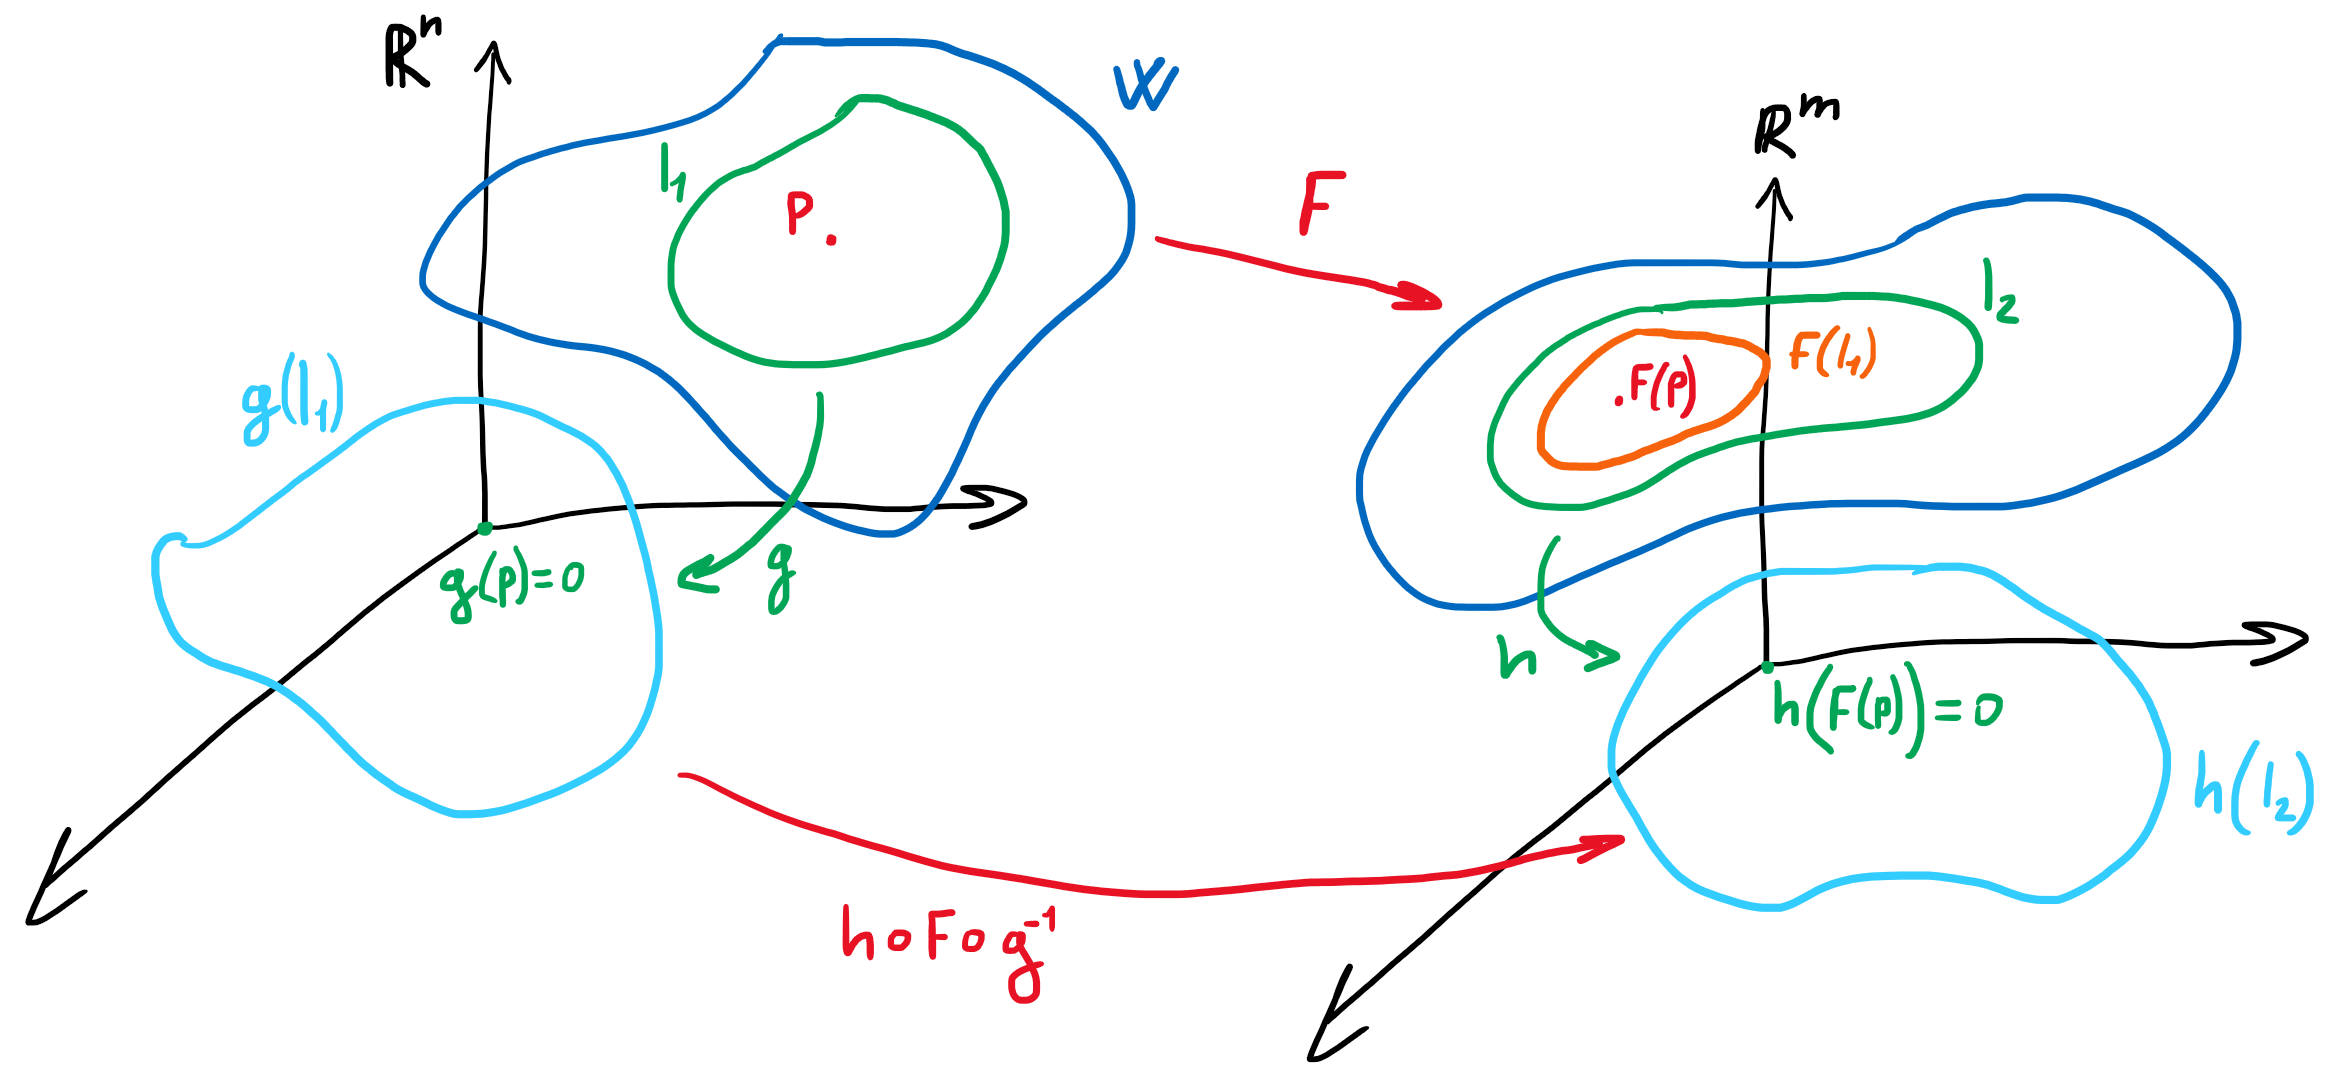
\includegraphics[width=0.7\textwidth,keepaspectratio]{img36}
	\end{figure}
\end{theorem}

\begin{theorem}[Rango costante in geometria differenziale]
	Siano $ F : N \to N $ un'applicazione liscia tra le varietà $ N $ ed $ M $ di dimensione rispettivamente $ n $ ed $ m $ e un intorno $ I $ di un punto $ p \in N $ tale che $ \rank(F(q)) = k \leqslant \min\{n,m\} $ per $ \forall q \in I $, allora esistono due carte $ (U,\phi) \in N $ centrata in $ p $ con $ \phi(p)=0 $ e $ (V,\psi) \in M $ centrata in $ F(p) $ con $ \psi(F(p))=0 $ tali che $ F(U) \subseteq V $ e la composizione tra le applicazioni delle carte ed $ F $ sia
	
	\begin{align}
		\begin{split}
			\psi \circ F \circ \phi^{-1} : \phi(U) &\to \psi(V)\\
			(r^{1},\dots,r^{n}) &\mapsto (r^{1},\dots,r^{k},0,\dots,0)
		\end{split}
	\end{align}

	dove $ \phi(U) \subset \R^{n} $ e $ \psi(V) \subset \R^{m} $, alternativamente scritta come
	
	\begin{equation}
		(\psi \circ F \circ \phi^{-1})(r^{1},\dots,r^{n}) = (r^{1},\dots,r^{k},0,\dots,0)
	\end{equation}
\end{theorem}

Questi teoremi derivano dal teorema della funzione inversa come caso particolare di quest'ultimo.

\begin{proof}
	La dimostrazione si basa sull'idea di restringere gli aperti considerati in modo tale che si possa applicare il teorema del rango costante in analisi.\\
	Consideriamo il seguente schema:
	
	\begin{figure}[H]
		\centering
		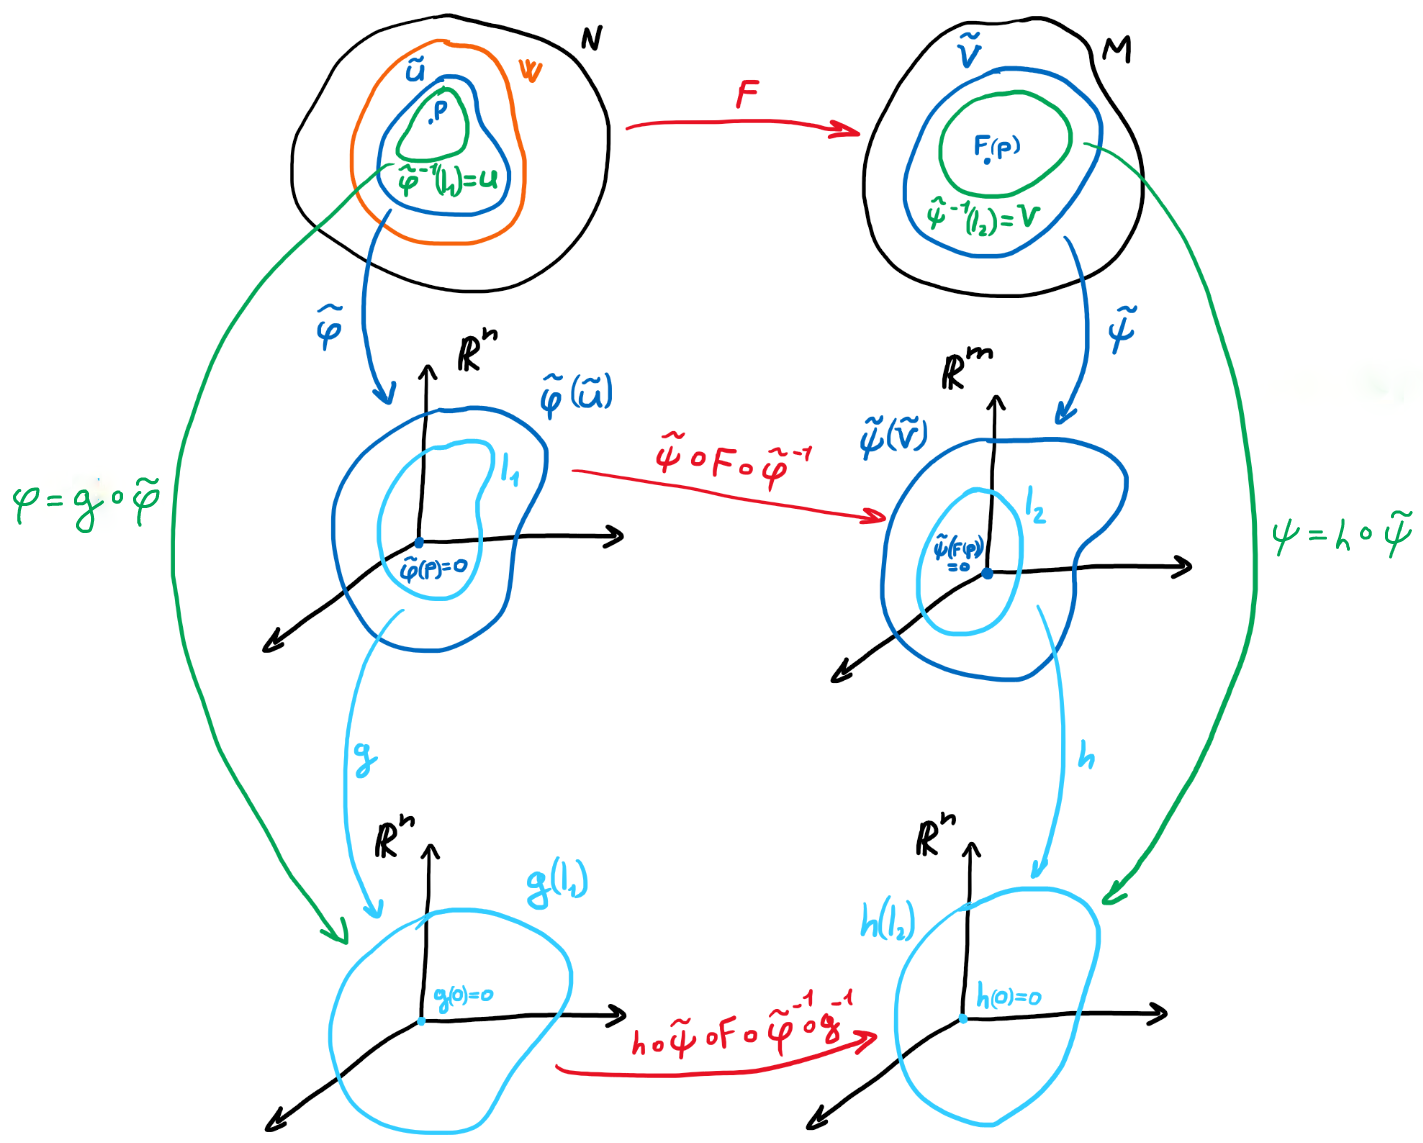
\includegraphics[width=\textwidth,keepaspectratio]{img37}
	\end{figure}

	Nell'intorno $ W \in N $ di $ p $ il rango di $ F $ è costante, i.e. $ \rank(F(q)) = k $ per $ \forall q \in W $. Consideriamo due carte arbitrarie $ (\tilde{U},\tilde{\phi}) \in N $ e $ (\tilde{V},\tilde{\psi}) \in M $ tali che $ F(\tilde{U}) \subseteq \tilde{V} $ e $ \tilde{\phi}(p) = 0 $ e $ \tilde{\psi}(F(p)) = 0 $, possiamo dunque scrivere la composizione
	
	\begin{equation}
		f = \tilde{\psi} \circ F \circ \tilde{\phi}^{-1} : \tilde{\phi}(\tilde{U}) \to \tilde{\psi}(\tilde{V})
	\end{equation}

	con $ \tilde{\phi}(\tilde{U}) \subset \R^{n} $ e $ \tilde{\psi}(\tilde{V}) \subset \R^{m} $; questa applicazione porta $ 0 \in \tilde{\phi}(\tilde{U}) $ in $ 0 \in \tilde{\psi}(\tilde{V}) $, in quanto entrambe le carte sono centrare rispettivamente in $ p $ e $ F(p) $.\\
	Essendo dominio e codominio di quest'applicazione due aperti di spazi euclidei, possiamo applicare il teorema del rango costante in analisi: sappiamo che
	
	\begin{equation}
		\rank(\tilde{\psi} \circ F \circ \tilde{\phi}^{-1})(\tilde{\phi}(q)) = k, \qquad \forall q \in \tilde{U}
	\end{equation}

	perciò esistono due aperti $ I_{1} \subset \tilde{\phi}(\tilde{U}) $ e $ I_{2} \subset \tilde{\psi}(\tilde{V}) $ entrambi centrati in nella rispettiva origine e due diffeomorfismi
	
	\begin{align}
		\begin{split}
			g : I_{1} &\to g(I_{1}) \subset \R^{n}\\
			h : I_{2} &\to h(I_{2}) \subset \R^{m}
		\end{split}
	\end{align}

	tali che $ g(0)=0 $ e $ h(0)=0 $, per i quali l'applicazione $ f $ può essere scirtta nella forma canonica
	
	\begin{align}
		\begin{split}
			h \circ f \circ g^{-1} : g(I_{1}) &\to h(I_{2})\\
			(r^{1},\dots,r^{n}) &\mapsto (r^{1},\dots,r^{k},0,\dots,0)
		\end{split}
	\end{align}

	A questo punto, possiamo considerare le carte
	
	\begin{align}
		\begin{split}
			(U,\phi) = (\tilde{\phi}(I_{1}),g \circ \tilde{\phi})\\
			(V,\psi) = (\tilde{\psi}(I_{2}),h \circ \tilde{\psi})
		\end{split}
	\end{align}

	centrate rispettivamente in $ p $ e $ F(p) $: esplicitando la composizione
	
	\begin{equation}
		h \circ f \circ g^{-1} = h \circ \tilde{\psi} \circ F \circ \tilde{\phi}^{-1} \circ g^{-1} = \psi \circ F \circ \phi^{-1}
	\end{equation}

	otteniamo dunque
	
	\begin{align}
		\begin{split}
			\psi \circ F \circ \phi^{-1} : \phi(U) &\to \psi(V)\\
			(r^{1},\dots,r^{n}) &\mapsto (r^{1},\dots,r^{k},0,\dots,0)
		\end{split}
	\end{align}
\end{proof}

\begin{theorem}[Preimmagine di un'applicazione di rango costante]
	Siano un'applicazione liscia $ F : N \to M $ tra le varietà differenziabili $ N $ e $ M $ di dimensione rispettivamente $ n $ ed $ m $ e un punto $ c \in M $ tale che $ F^{-1}(c) \neq \emptyset $ e supponiamo esista un aperto $ W \subset N $ tale che $ F^{-1}(c) \subset W $ nel quale il rango di $ F $ sia costante, i.e.
	
	\begin{equation}
		\rank(F(q))=k, \qquad \forall q \in W
	\end{equation}

	Allora $ F^{-1}(c) $ è una sottovarietà di $ N $ con $ \operatorname{cod}_{N}(F^{-1}(c)) = k $ o equivalentemente $ \dim(F^{-1}(c)) = n-k $.
\end{theorem}

\begin{proof}
	Sia un punto $ p \in F^{-1}(c) $, costruiamo dunque una carta di $ N $ intorno a $ p $ relativamente a $ F^{-1}(c) $. Siano le carte
	
	\begin{itemize}
		\item $ (U,\phi) \in N $ con $ \phi = (x^{1},\dots,x^{n}) $ centrata in $ p $, i.e. $ \phi(p) = 0 \in \R^{n} $;
		
		\item $ (V,\psi) \in M $ con $ \psi = (y^{1},\dots,y^{m}) $ centrata in $ F(p) = c $, i.e. $ \psi(F(p)) = 0 \in \R^{m} $
	\end{itemize}

	tali che $ F(U) \subseteq V $ (in quanto $ F $ è continua) e
	
	\begin{align}
		\begin{split}
			\psi \circ F \circ \phi^{-1} : \phi(U) &\to \psi(V)\\
			(r^{1},\dots,r^{n}) &\mapsto (r^{1},\dots,r^{k},0,\dots,0)
		\end{split}
	\end{align}

	dove $ \phi(U) \subset \R^{n} $ e $ \psi(V) \subset \R^{m} $. Questa carte esistono perché possiamo supporre che $ U \subset W $ dove $ W $ è un intorno di $ p $ in cui il rango di $ F $ è costante con valore $ k $.\\
	Osserviamo che
	
	\begin{align}
		\begin{split}
			(\psi \circ F \circ \phi^{-1})^{-1}(0) &= \{ \phi(q) \in \phi(U) \mid r^{1}(\phi(q)) = \cdots = r^{k}(\phi(q)) = 0 \}\\
			&= \{ \phi(q) \in \phi(U) \mid x^{1}(q) = \cdots = x^{k}(q) = 0 \}
		\end{split}
	\end{align}

	siccome $ F \equiv F_{|U} $
	
	\begin{align}
		\begin{split}
			(\psi \circ F \circ \phi^{-1})^{-1}(0) &= (\psi \circ F_{|U} \circ \phi^{-1})^{-1}(0) \\
			&= (\phi \circ F_{|U}^{-1} \circ \psi^{-1})(0)\\
			&= \phi( \, F_{|U}^{-1}(\psi^{-1}(0)) \, )\\
			&= \phi( \, F_{|U}^{-1}(F(p)) \, )\\
			&= \phi( F_{|U}^{-1}(c) )\\
			&= \phi( U \cap F^{-1}(c) )
		\end{split}
	\end{align}

	dunque
	
	\begin{equation}
		\phi( U \cap F^{-1}(c) ) = \{ \phi(q) \in \phi(U) \mid x^{1}(q) = \cdots = x^{k}(q) = 0 \}
	\end{equation}

	facendo la controimmagine di questo insieme tramite $ \phi $ otteniamo
	
	\begin{equation}
		U \cap F^{-1}(c) = \{ q \in U \mid x^{1}(q) = \cdots = x^{k}(q) = 0 \}
	\end{equation}

	la quale è la condizione per cui $ (U,\phi) $ è una carta adattata di $ N $ intorno a $ p $ (arbitrario) relativamente a $ F^{-1}(c) $, rendendo perciò $ F^{-1}(c) $ una sottovarietà di $ N $ di dimensione $ n-k $.
\end{proof}

\subsubsection{\textit{Esempio}}

Dimostriamo che l'insieme delle matrici ortogonali

\begin{equation}
	O(n) = \{ A \in GL_{n}(\R) \mid A^{T} A = I_{n} \} \subset GL_{n}(\R)
\end{equation}

è una sottovarietà di $ GL_{n}(\R) $.\\
Sia l'applicazione

\begin{align}
	\begin{split}
		F : GL_{n}(\R) &\to GL_{n}(\R)\\
		A &\mapsto A^{T} A
	\end{split}
\end{align}

dunque $ O(n) = F^{-1}(I) $ dove $ I = I_{n} $.\\
Introduciamo le applicazioni traslazione a sinistra e a destra:

\begin{align}
	\begin{split}
		L_{C} : GL_{n}(\R) &\to GL_{n}(\R)\\
		A &\mapsto C A\\\\
		%
		R_{C} : GL_{n}(\R) &\to GL_{n}(\R)\\
		A &\mapsto A C
	\end{split}
\end{align}

le quali sono diffeomorfismi con inverse $ L_{C}^{-1} = L_{C^{-1}} $ e $ R_{C}^{-1} = R_{C^{-1}} $. Vale la seguente equazione

\begin{equation}
	L_{C^{T}} \circ R_{C} \circ F = F \circ R_{C}
\end{equation}

in quanto

\begin{align}
	\begin{split}
		(F \circ R_{C})(A) &= F(AC)\\
		&= (AC)^{T} (AC)\\
		&= C^{T} A^{T} A C\\
		&= C^{T} F(A) C\\
		&= (L_{C^{T}} \circ R_{C} \circ F)(A)
	\end{split}
\end{align}

Considerando $ A \in GL_{n}(\R) $, calcoliamo il differenziale dell'equazione

\begin{align}
	\begin{split}
		(L_{C^{T}} \circ R_{C} \circ F)_{*A} &= (F \circ R_{C})_{*A}\\
		L_{C^{T}_{*A^{T} A C}} \circ R_{C_{*A^{T} A}} \circ F_{*A} &= F_{*A C} \circ R_{C_{*A}}
	\end{split}
\end{align}

Siccome le traslazioni a sinistra e a destra sono diffeomorfismi, i loro differenziali sono isomorfismi, i quali non modificano il rango di applicazioni lineari, perciò

\begin{equation}
	\rank(F_{*A}) = \rank(F_{*A C})
\end{equation}

da cui, essendo $ C $ arbitrario, possiamo scrivere $ A C = B $ e

\begin{equation}
	\rank(F(A)) = \rank(F(B)), \qquad \forall A,B \in GL_{n}(\R)
\end{equation}

dunque il rango di $ F $ non dipende dalla matrice a cui si applica, i.e. il rango di $ F $ è costante in tutto $ GL_{n}(\R) $.\\
Applicando dunque il teorema, $ O(n) $ è una sottovarietà di $ GL_{n}(\R) $.

\subsection{Teoremi di immersione e sommersione locale}

Un'applicazione liscia $ F : N \to M $ tra varietà differenziabili di dimensione rispettivamente $ n $ ed $ m $ ha \textit{rango massimale} in un punto $ p \in N $ se

\begin{equation}
	\rank(F(p)) = k = \min\{n,m\}
\end{equation}

Se $ k = m \leqslant n $ allora $ F $ è una sommersione ($ F_{*p} $ suriettivo) in $ p $ invece se $ k = n \leqslant m $ allora $ F $ è un'immersione ($ F_{*p} $ iniettivo) in $ p $.

\begin{lemma}
	Sia un'applicazione liscia $ F : N \to M $ e sia $ p \in N $ tale che il rango di $ F $ in $ p $ sia massimale, allora esiste un intorno di $ p $ dove il rango di $ F $ è massimale. Equivalentemente, la condizione di \textit{rango massimale} è una \textit{condizione aperta}.
\end{lemma}

\begin{proof}
	Siano le carte $ (U,\phi) \in N $ con $ \phi = (x^{1},\dots,x^{n}) $ centrata in $ p $ e $ (V,\psi) \in M $ con $ \psi = (y^{1},\dots,y^{m}) $ centrata in $ F(p) $ tali che $ F(U) \subseteq V $ e definiamo l'insieme
	
	\begin{equation}
		W \doteq \{ q \in U \mid \rank(J(F)(q)) = \rank \left( \left[ \dfrac{\partial F^{i}}{\partial x^{j}} (q) \right] \right) = k \}
	\end{equation}

	Per ipotesi $ p \in W $ e dunque $ W \neq \emptyset $. Mostriamo che $ W $ è aperto in $ U $: siccome $ U $ è aperto in $ N $, allora anche $ W $ sarà aperto in $ N $.\\
	Possiamo riscrivere $ W $ con $ \rank(J(F)(q)) \geqslant k $ perché il rango è massimale e non può essere $ >k $, dunque le condizioni sono equivalenti, i.e.
	
	\begin{equation}
		W = \{ q \in U \mid \rank(J(F)(q)) \geqslant k \}
	\end{equation}

	Il complementare di $ W $ è
	
	\begin{align}
		\begin{split}
			U \setminus W &= \{ q \in U \mid \rank(J(F)(q)) < k \}\\
			&= \{ q \in U \mid m_{1}(q) = \cdots = m_{t}(q) = 0 \}
		\end{split}
	\end{align}

	dove i $ m_{i}(q) $ sono i minori di ordine $ k $ di $ J(F)(q) $ e
	
	\begin{equation}
		t =%
			\begin{cases}
				\binom{m}{k} & k = n\\\\
				\binom{n}{k} & k = m
			\end{cases}
	\end{equation}

	Essendo i minori delle funzioni continue e $ U \setminus W $ la controimmagine di 0 (chiuso) del sistema finito di $ t $ funzioni continue
	
	\begin{equation}
		\begin{cases}
			m_{1}(q) = 0\\
			\vdots\\
			m_{t}(q) = 0
		\end{cases}
	\end{equation}

	o equivalentemente la controimmagine di 0 della funzione continua
	
	\begin{align}
		\begin{split}
			f : U &\to \R^{t}\\
			q &\mapsto (m_{1}(q),\dots,m_{t}(q))
		\end{split}
	\end{align}

	allora l'insieme $ U \setminus W = f^{-1}(0) $ è chiuso e dunque il suo complementare $ W $ è aperto.
\end{proof}

\begin{remark}
	Preso un intorno $ I $ di un punto $ p $, abbiamo che
	
	\begin{align}
		\begin{split}
			\rank(F(p)) = k \text{ massimale} &\implies \rank(F(q)) = k \text{ costante}\\
			\rank(F(p)) = k \text{ costante} &\notimplies \rank(F(p)) = k \text{ massimale}
		\end{split}
	\end{align}

	per $ \forall q \in I $.
\end{remark}

\begin{corollary}
	Sia $ F : N \to M $ un'immersione in $ p \in N $ ($ F_{*p} $ iniettivo), allora $ F $ è un'immersione in un intorno di $ p $. Analogamente, se $ F $ è una sommersione in $ p $, allora $ F $ è una sommersione in un intorno di $ p $.\\
	Questo significa che la condizione per un'applicazione di essere un'immersione o una sommersione è una condizione aperta.
\end{corollary}

\begin{proof}
	Essendo il rango dell'applicazione $ F $ massimale in $ p $ per un'immersione (risp. sommersione), esiste un intorno di $ p $ in cui il rango è costantemente uguale al massimo, dunque l'applicazione continua ad essere un'immersione (risp. sommersione) anche in questo intorno.
\end{proof}

Combinando questo corollario con il teorema del rango costante si ottengono i teoremi di immersione e sommersione locale.

\begin{theorem}[Immersione locale]\label{loc-imm}
	Sia $ F : N \to M $ ($ n \leqslant m $) un'immersione in $ p \in N $, allora esistono due carte $ (U,\phi) \in N $ con $ \phi = (x^{1},\dots,x^{n}) $ e $ \phi(p)=0 $ e $ (V,\psi) \in M $ con $ \psi = (y^{1},\dots,y^{m}) $ e $ \psi(F(p))=0 $ tali che $ F(U) \subseteq V $ e la funzione può essere scritta come \textit{immersione canonica} (inclusione)
	
	\begin{align}
		\begin{split}
			\psi \circ F \circ \phi^{-1} : \phi(U) &\to \psi(V)\\
			(r^{1},\dots,r^{n}) &\mapsto (r^{1},\dots,r^{n},0,\dots,0)
		\end{split}
	\end{align}

	dove nell'immagine ci sono $ m-n $ zeri.
\end{theorem}

\begin{theorem}[Sommersione locale]\label{loc-sub}
	Sia $ F : N \to M $ ($ n \geqslant m $) una sommersione in $ p \in N $, allora esistono due carte $ (U,\phi) \in N $ con $ \phi = (x^{1},\dots,x^{n}) $ e $ \phi(p)=0 $ e $ (V,\psi) \in M $ con $ \psi = (y^{1},\dots,y^{m}) $ e $ \psi(F(p))=0 $ tali che $ F(U) \subseteq V $ e la funzione può essere scritta come \textit{sommersione canonica} (proiezione)
	
	\begin{align}
		\begin{split}
			\psi \circ F \circ \phi^{-1} : \phi(U) &\to \psi(V)\\
			(r^{1},\dots,r^{n}) &\mapsto (r^{1},\dots,r^{m})
		\end{split}
	\end{align}
	
	dove nell'immagine ci sono le prime $ m $ coordinate del punto del dominio.
\end{theorem}

\begin{corollary}[1]\label{th-somm-loc-cor}
	Sia $ F : N \to M $ una sommersione, allora $ F $ è un'applicazione aperta.
\end{corollary}

\begin{proof}
	La sommersione è localmente aperta in quanto la sommersione canonica è un'applicazione aperta, ma un'applicazione localmente aperta è anche aperta. Infatti, se $ U \subset N $ è aperto e $ F $ è localmente aperta, allora
	
	\begin{equation}
		\forall p \in U, \, \E U_{p} \text{ intorno} \mid F_{|U_{p}} \text{ aperta}
	\end{equation}

	ma $ U $ si può scrivere come
	
	\begin{equation}
		U = \bigcup_{p \in U} U_{p}
	\end{equation}

	e applicando $ F $ si ottiene
	
	\begin{align}
		F(U) = F \left( \bigcup_{p \in U} U_{p} \right) = \bigcup_{p \in U} F(U_{p})
	\end{align}

	che è aperto in quanto unione di aperti.
\end{proof}

\begin{corollary}[2]
	Sia $ F : N \to M $ una sommersione tra varietà $ N $ compatta e $ M $ connessa, allora $ F $ è suriettiva.
\end{corollary}

\begin{proof}
	Per il primo corollario, $ F $ è aperta in quanto sommersione, mentre per il lemma dell'applicazione chiusa\footnote{%
		Vedi Lemma \ref{lemma-clos-app}.%
	} $ F $ è anche chiusa. A questo punto, l'immagine di $ N $ attraverso $ F $ è sia aperta che chiusa ma è sottoinsieme di $ M $ che è compatto ($ F(N) \subseteq M $): l'unico sottoinsieme di un compatto che è sia aperto che chiuso è il compatto stesso, dunque $ F(N) = M $ e perciò $ F $ è suriettiva.
\end{proof}

\begin{corollary}[3]
	Siano $ N $ una varietà differenziabile compatta e $ F : N \to \R^{m} $ un'applicazione liscia, allora deve esistere almeno un punto critico, i.e. $ \mathcal{PC}_{F} \neq \emptyset $.
\end{corollary}

\begin{proof}
	Se per assurdo $ \mathcal{PC}_{F} = \emptyset $ allora $ N = \mathcal{PR}_{F} $ e quindi $ F $ è una sommersione: per il secondo corollario $ F(N) = \R^{m} $ ma questo è assurdo in quanto $ N $ è compatta e dunque la sua immagine è compatta mentre $ \R^{m} $ non lo è (un'applicazione suriettiva porta compatti in compatti).
\end{proof}

\begin{corollary}[4]\label{imm_sph}
	Non esiste un'immersione dalla sfera $ \S^{n} $ a $ \R^{n} $.
\end{corollary}

\begin{proof}
	Se per assurdo esistesse un'immersione $ F : \S^{n} \to \R^{n} $ allora, siccome le dimensioni di dominio e codominio sono uguali, questa sarebbe anche una sommersione, in contrasto con il terzo corollario.
\end{proof}

\begin{remark}
	L'affermazione
	
	\begin{equation}
		F : N \to M \text{ liscia} \wedge c \in \mathcal{VR}_{F} \cap F(N) \implies F^{-1}(c) \text{ sottovarietà di } N
	\end{equation}

	segue dall'affermazione
	
	\begin{gather}
		F : N \to M \text{ liscia} \wedge \rank(F(q)) = k, \, \forall q \in W \supset F^{-1}(c)\nonumber\\
		\Downarrow\\
		F^{-1}(c) \text{ sottovarietà di } N\nonumber
	\end{gather}
\end{remark}

\begin{proof}
	Consideriamo la funzione $ F : N \to M $ il punto $ c \in \mathcal{VR}_{F} \cap F(N) $ dunque un punto $ p $ della controimmagine di $ c $ apparterrà a $ p \in \mathcal{PR}_{F} \cap F^{-1}(c) $. Siccome $ p $ è un punto regolare, $ F $ è una sommersione in $ p $ ($ n \geqslant m $): essendo la condizione di sommersione in un punto una condizione aperta, esiste un intorno $ U_{p} \subset N $ di $ p $ tale che
	
	\begin{equation}
		\rank(F(q)) = m, \qquad \forall q \in U_{p}
	\end{equation}
	
	Il rango della funzione $ F $ è massimale ($ m = \dim(M) $) in quanto F è una sommersione ed è costante nell'aperto $ U_{p} $ in quanto massimale in $ p $ (la condizione di rango massimale è aperta).\\
	A questo punto, al variare di $ p $, abbiamo diversi aperti di cui consideriamo l'unione
	
	\begin{equation}
		W = \bigcup_{p \in \mathcal{PR}_{F} \cap F^{-1}(c)} U_{p}
	\end{equation}
	
	la quale contiene $ F^{-1}(c) $, i.e. $ W \supset F^{-1}(c) $.\\
	Avendo considerato l'unione di aperti in cui il rango è costante (e massimale), questo sarà ancora costante (e massimale) in tutto $ W $, i.e.
	
	\begin{equation}
		\rank(F(q)) = m, \qquad \forall q \in W
	\end{equation}

	il che implica
	
	\begin{equation}
		\rank(F(q)) = m, \qquad \forall q \in F^{-1}(c)
	\end{equation}
	
	in quanto $ F^{-1}(c) \subset W $: per il teorema della preimmagine di un'applicazione di rango costante, otteniamo dunque che $ F^{-1}(c) $ è una sottovarietà di $ N $.\\	
	Questo dimostra l'implicazione in quanto abbiamo mostrato che il teorema della preimmagine di un valore regolare segue dal teorema della preimmagine di un'applicazione di rango costante, in quanto abbiamo usato il secondo teorema per dimostrare il primo.
\end{proof}

\subsection{Immagini di applicazioni lisce}

Ci chiediamo sotto quali ipotesi l'immagine di una varietà differenziabile $ N $ attraverso un'applicazione liscia $ F : N \to M $, i.e. F(N), è una sottovarietà di $ M $.\\
Supponiamo che $ N \subset M $ sia una sottovarietà, allora l'inclusione canonica

\begin{align}
	\begin{split}
		i : N &\to M\\
		q &\mapsto q
	\end{split}
\end{align}

è un'immersione iniettiva e un \textit{embedding topologico}\footnote{%
	Un embedding topologico è un'applicazione $ f : N \to M $ che individua un omeomorfismo tra $ N $ e $ f(N) $ dove quest'ultimo ha la topologia ereditata da $ M $.%
} (la condizione di embedding topologico implica l'iniettività).\\
Da questa inclusione, possiamo definire l'\textit{embedding differenziale}\footnote{%
	L'"embedding differenziale" verrà indicato semplicemente come "embedding", altrimenti verrà esplicitato "embedding topologico" nel caso in cui saremo interessati solo agli aspetti topologici.%
} come un'applicazione liscia $ F : N \to M $ che soddisfa le seguenti due condizioni:

\begin{itemize}
	\item $ F $ è un'immersione
	
	\item $ F $ è un embedding topologico
\end{itemize}

il che implica che un embedding è iniettivo. Ad esempio, come visto sopra, l'inclusione canonica è un embedding.

\begin{theorem}\label{emb-subv}
	Sia $ F : N \to M $ un embedding differenziabile, allora $ F(N) $ è una sottovarietà di $ M $ con $ \dim(N) = \dim(F(N)) $, dove $ F(N) \stackrel{diff.}{\simeq} N $ in quanto l'embedding induce un diffeomorfismo.
\end{theorem}

\begin{proof}
	La dimostrazione sfrutta il teorema di immersione locale: essendo $ F : N \to M $ un'immersione ($ n \leqslant m $), dato $ p \in N $, esistono due carte $ (U,\phi) \in N $ con $ \phi = (x^{1},\dots,x^{n}) $ e $ \phi(p)=0 $ e $ (V,\psi) \in M $ con $ \psi = (y^{1},\dots,y^{m}) $ e $ \psi(F(p))=0 $ tali che $ F(U) \subseteq V $ e
	
	\begin{align}
		\begin{split}
			\psi \circ F \circ \phi^{-1} : \phi(U) &\to \psi(V)\\
			(r^{1},\dots,r^{n}) &\mapsto (r^{1},\dots,r^{n},0,\dots,0)
		\end{split}
	\end{align}

	dove $ \phi(U) \subset \R^{n} $, $ \psi(V) \subset \R^{m} $ e nell'immagine ci sono $ m-n $ zeri.\\
	Applicando la funzione a $ \phi(U) $ otteniamo
	
	\begin{align}
		\begin{split}
			(\psi \circ F \circ \phi^{-1})(\phi(U)) &= \{ \psi(q) \in \psi(V) \mid r^{n+1}(\psi(q)) = \cdots = r^{m}(\psi(q)) = 0 \}\\
			\psi(F(U)) &= \{ \psi(q) \in \psi(V) \mid y^{n+1}(q) = \cdots = y^{m}(q) = 0 \}\\
			F(U) &= \{ q \in V \mid y^{n+1}(q) = \cdots = y^{m}(q) = 0 \}
		\end{split}
	\end{align}

	Avremmo che $ (V,\psi) $ è una carta adattata di $ M $ intorno a $ F(p) $ relativamente a $ F(N) $ se $ F(N) \cap V = F(U) $ ma, in generale questa uguaglianza è falsa: può capitare semplicemente che $ F(U) \subsetneqq F(N) \cap V $ e questa condizione non è sufficiente perché $ V $ sia una carta adattata. Ad esempio, considerando lo schema
	
	\begin{figure}[H]
		\centering
		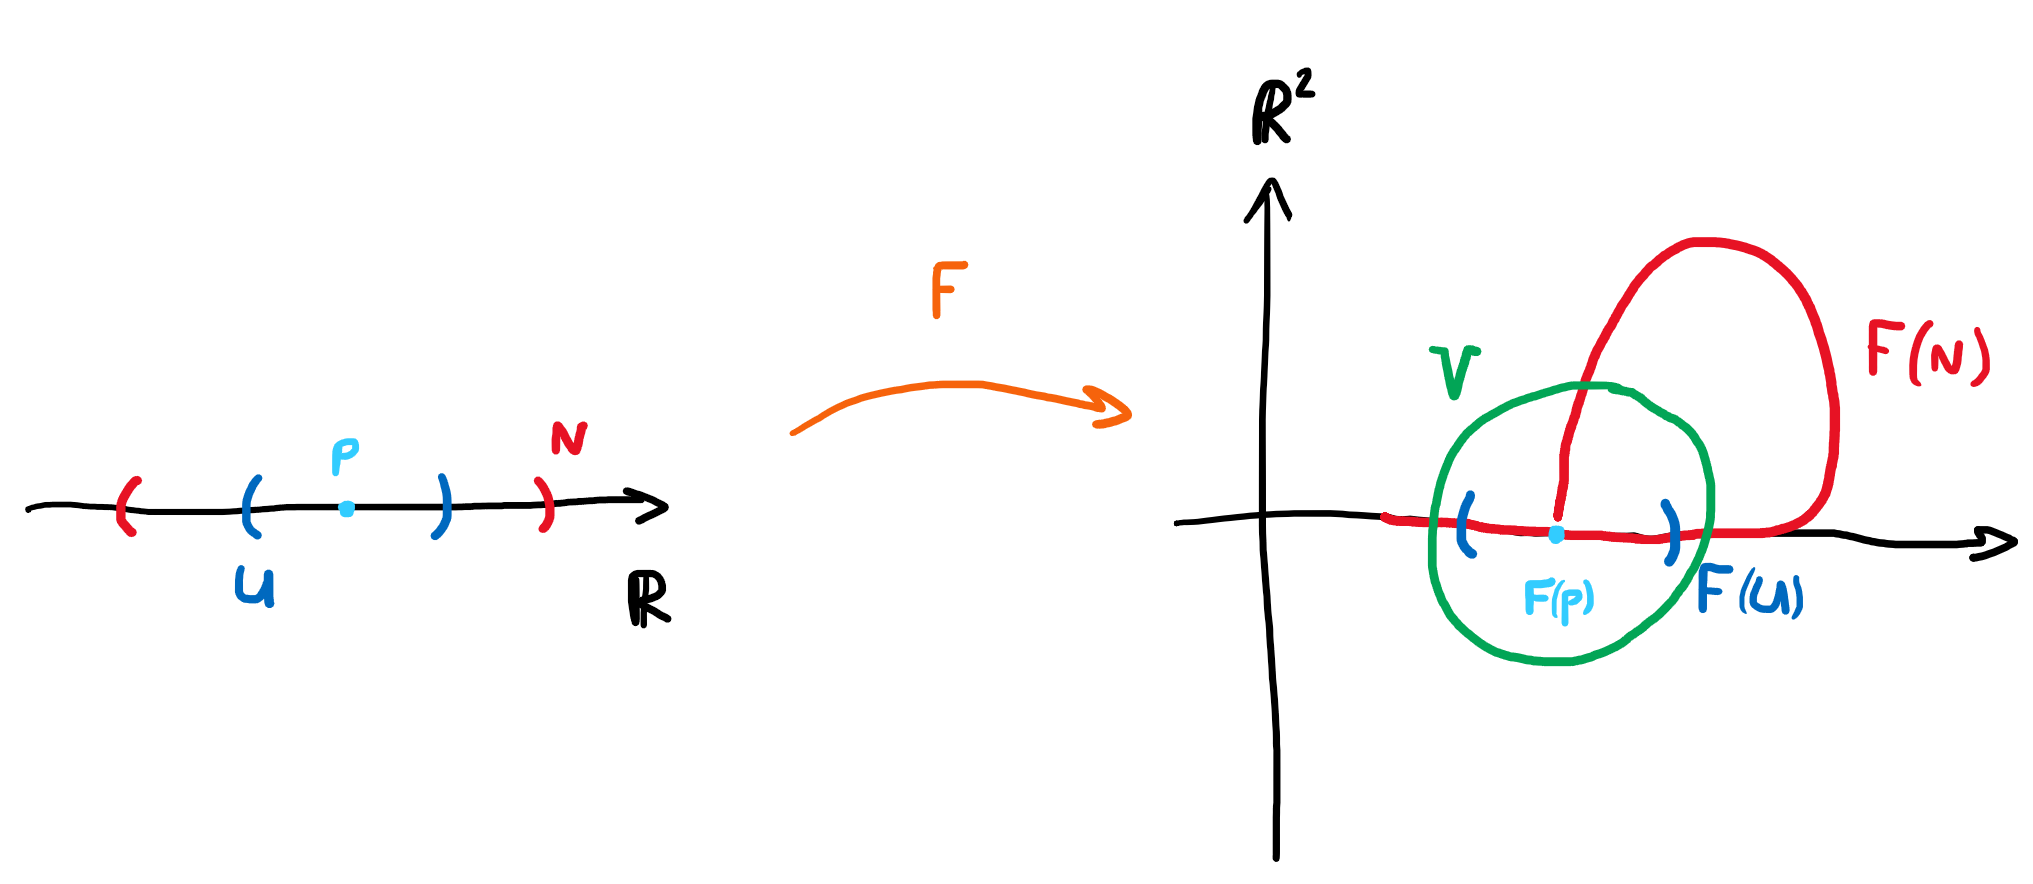
\includegraphics[width=0.7\textwidth,keepaspectratio]{img38}
	\end{figure}
	
	vediamo che, siccome un'estremità di $ F(N) $ si avvicina indefinitamente a $ F(p) $ senza toccarlo, $ F(U) \subset F(N) \cap V $ ma non è possibile trovare un aperto $ V \in \R^{2} $ tale che $ F(U) = F(N) \cap V $.\\
	Sfruttando ora il fatto che $ F $ sia anche un'embedding topologico, sappiamo che $ F(U) $ è un aperto di $ F(N) \subset M $, cioè esiste un aperto $ V' \subset M $ tale che $ F(U) = F(N) \cap V' $ (questo perché la topologia di $ F(N) $ è indotta da $ M $). Intersecando l'uguaglianza con l'aperto $ V $ della carta e chiamando $ W \doteq V \cap V' $, otteniamo
	
	\begin{equation}
		F(U) \cap V = F(N) \cap V' \cap V = F(N) \cap W
	\end{equation}

	siccome $ F(U) \subseteq V $ abbiamo che $ F(U) \cap V = F(U) $, perciò
	
	\begin{equation}
		F(N) \cap W = \{ q \in V \mid y^{n+1}(q) = \cdots = y^{m}(q) = 0 \}
	\end{equation}

	dalla definizione di $ F(U) $ sopra e dunque $ (W,\psi_{|W}) $ è una carta adattata di $ M $ intorno a $ F(p) $ relativamente a $ F(N) $ (restringendo l'aperto da $ V $ e $ W $, si ottiene la definizione per le sottovarietà). A questo punto, dato che il punto $ p $ è arbitrario, $ F(N) $ è una sottovarietà di $ M $ di dimensione $ n $.
\end{proof}

\begin{remark}[1]
	Se $ F : N \to M $ è un'immersione iniettiva, questo non implica che $ F(N) $ sia una sottovarietà di $ M $. Chiameremo dunque $ F(N) \subset M $ \textit{sottovarietà immersa}\footnote{%
		Una sottovarietà immersa non è necessariamente una sottovarietà.%
	}, la quale è diffeomorfa a $ N $ ma non ha la struttura differenziale ereditata da $ M $.
\end{remark}

\begin{remark}[2]
	Se $ F : N \to M $ è un'immersione iniettiva ed $ N $ è compatta allora $ F $ è un embedding. Per il lemma dell'applicazione chiusa\footnote{%
		Vedi Lemma \ref{lemma-clos-app}.%
	}, essendo $ F $ continua e $ M $ compatta segue che $ F : N \to F(N) $ è un omeomorfismo e quindi un embedding topologico.
\end{remark}

\begin{theorem}[Whitney]
	Se $ N $ è una varietà differenziabile di dimensione $ n $ allora esiste $ F : N \to \R^{2n} $ embedding differenziabile.\\
	Questo significa che $ F(N) $, identificabile con $ N $ tramite il diffeomorfismo $ F $, è una sottovarietà di $ \R^{2n} $.
\end{theorem}

\begin{theorem}[Whitney (forma debole)]
	Se $ N $ è una varietà differenziabile di dimensione $ n>1 $ allora esiste esiste $ F : N \to \R^{2n-1} $ immersione iniettiva.
\end{theorem}

Nel caso in cui $ n=1 $, non esiste un'immersione iniettiva tra $ N $ e $ \R $, e.g. tra $ \S^{1} $ e $ \R $\footnote{%
	Vedi Corollario \ref{imm_sph}.%
}.\\
Vedi Esercizio \ref{es2-23}.

\subsubsection{\textit{Esempi}}

\paragraph{1)}

Nell'esempio della dimostrazione del Teorema \ref{emb-subv}, $ F(N) $ non può essere una sottovarietà di $ \R^{2} $ in quanto, avendo la topologia indotta da quest'ultima, non è localmente euclideo: un qualunque intorno di $ F(p) $ non è omeomorfo a $ \R^{n} $ in quanto il primo, togliendo il punto $ F(p) $, è formato da tre componenti connesse mentre il secondo può essere o formato da due componenti connesse (per $ \R $) o è connesso.

\paragraph{2) Cuspide cubica}

Sia l'applicazione della cuspide cubica $ y^{2} = x^{3} $ (cubica)

\begin{align}
	\begin{split}
		F : \R &\to \R^{2}\\
		t &\mapsto (x,y) = (t^{2},t^{3})
	\end{split}
\end{align}

Questa è iniettiva perché per due punti dell'immagine uguali otteniamo che

\begin{equation}
	(t_{1}^{2},t_{1}^{3}) = (t_{2}^{2},t_{2}^{3})%
	\implies%
	\begin{cases}
		t_{1}^{2} = t_{2}^{2}\\
		t_{1}^{3} = t_{2}^{3}
	\end{cases}%
	\implies%
	\begin{cases}
		t_{1} = \pm t_{2}\\
		t_{1} = t_{2}
	\end{cases}%
	\implies%
	t_{1} = t_{2}
\end{equation}

Per controllare se sia un'immersione, dobbiamo controllare che il differenziale sia iniettivo e dunque che lo jacobiano abbia rango massimale (unitario in questo caso):

\begin{equation}
	J(F) = \begin{pmatrix} 2t \\ 3t^{2} \end{pmatrix}
\end{equation}

dunque non è un'immersione perché nell'origine per $ t=0 $ il differenziale non è iniettivo.\\
Non è nemmeno un embedding in quanto la cuspide cubica non è una sottovarietà di $ \R^{2} $.\\
Con un abuso di nomenclatura, si potrebbe dire che la cuspide cubica è una "sottovarietà topologica" di $ \R^{2} $ in quanto totalmente omeomorfa (anche nell'origine) a $ \R $ e questo rende $ F $ un embedding topologico.

\paragraph{3) Cubica nodale}

Sia l'applicazione della cubica nodale $ y^{2} = x^{3} + x^{2} $ (cubica)

\begin{align}
	\begin{split}
		F : \R &\to \R^{2}\\
		t &\mapsto (x,y) = (t^{2}-1,t^{3}-t)
	\end{split}
\end{align}

\begin{figure}[H]
	\centering
	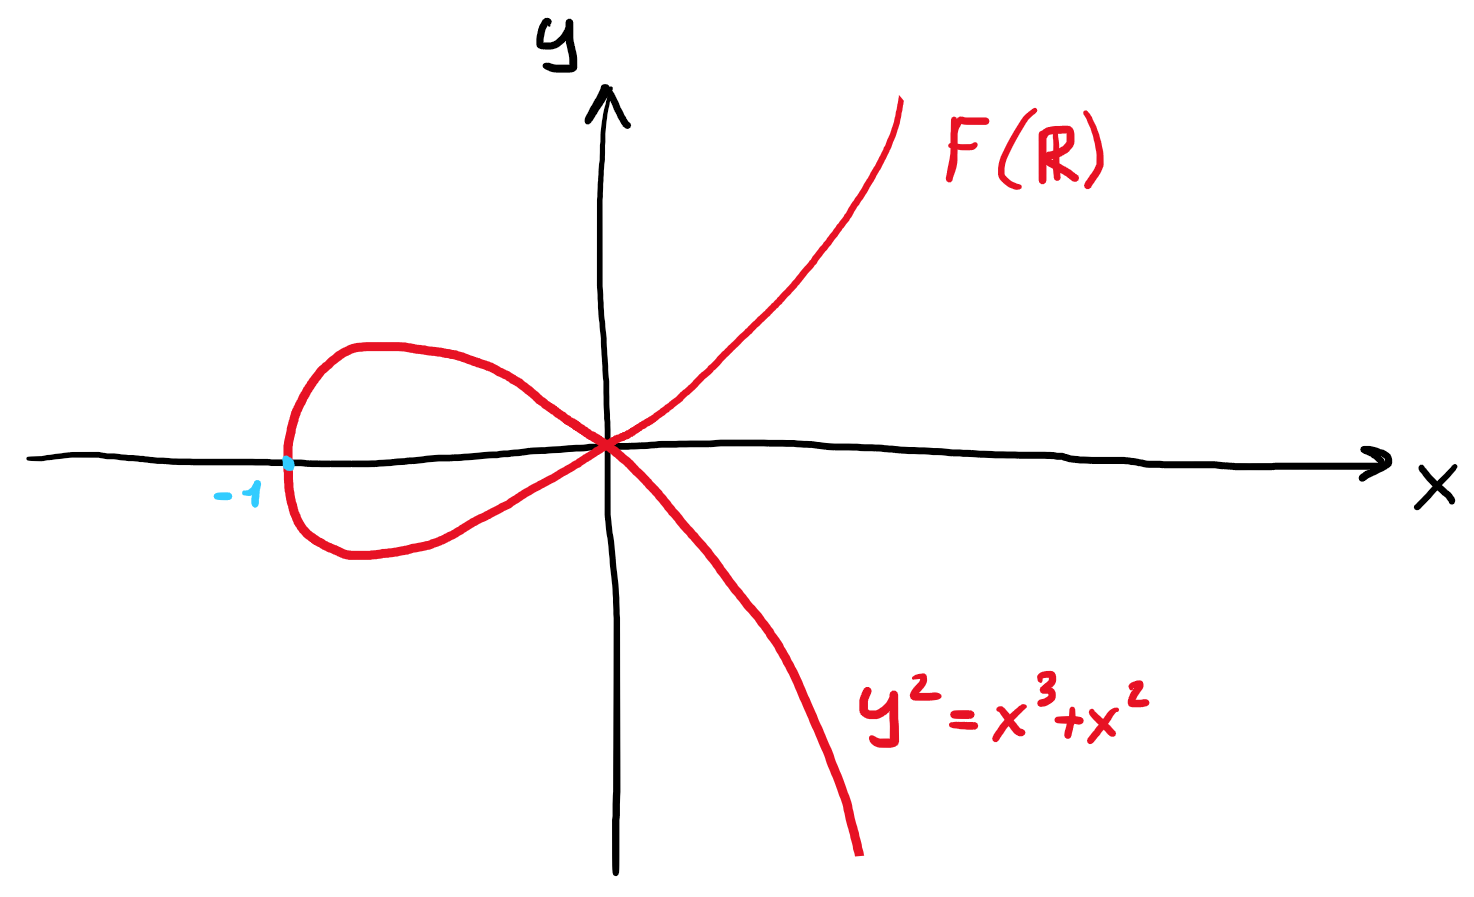
\includegraphics[width=0.5\textwidth,keepaspectratio]{img39}
\end{figure}

Questa non è iniettiva perché per esempio $ F(\pm 1) $ = 0, dunque non è nemmeno un embedding topologico.\\
Per controllare se sia un'immersione, cerchiamo un punto che annulla contemporaneamente le derivate di $ F $ rispetto a $ t $:

\begin{equation}
	\dot{F}(t) = (2t, 3 t^{2} - 1) \neq (0,0), \qquad \forall t \in \R
\end{equation}

dunque $ F $ è un'immersione.\\
Anche la cuspide cubica non è localmente euclidea nell'origine, dunque non può essere una sottovarietà di $ \R^{2} $.

\paragraph{4) Lemniscata di Bernoulli}

Sia l'applicazione della lemniscata di Bernoulli $ x^{2} = 4 y^{2} (1-y^{2}) $ (quartica)

\begin{align}
	\begin{split}
		F : (-\pi,\pi) &\to \R^{2}\\
		t &\mapsto (x,y) = (\sin(2t),\sin(t))
	\end{split}
\end{align}

\begin{figure}[H]
	\centering
	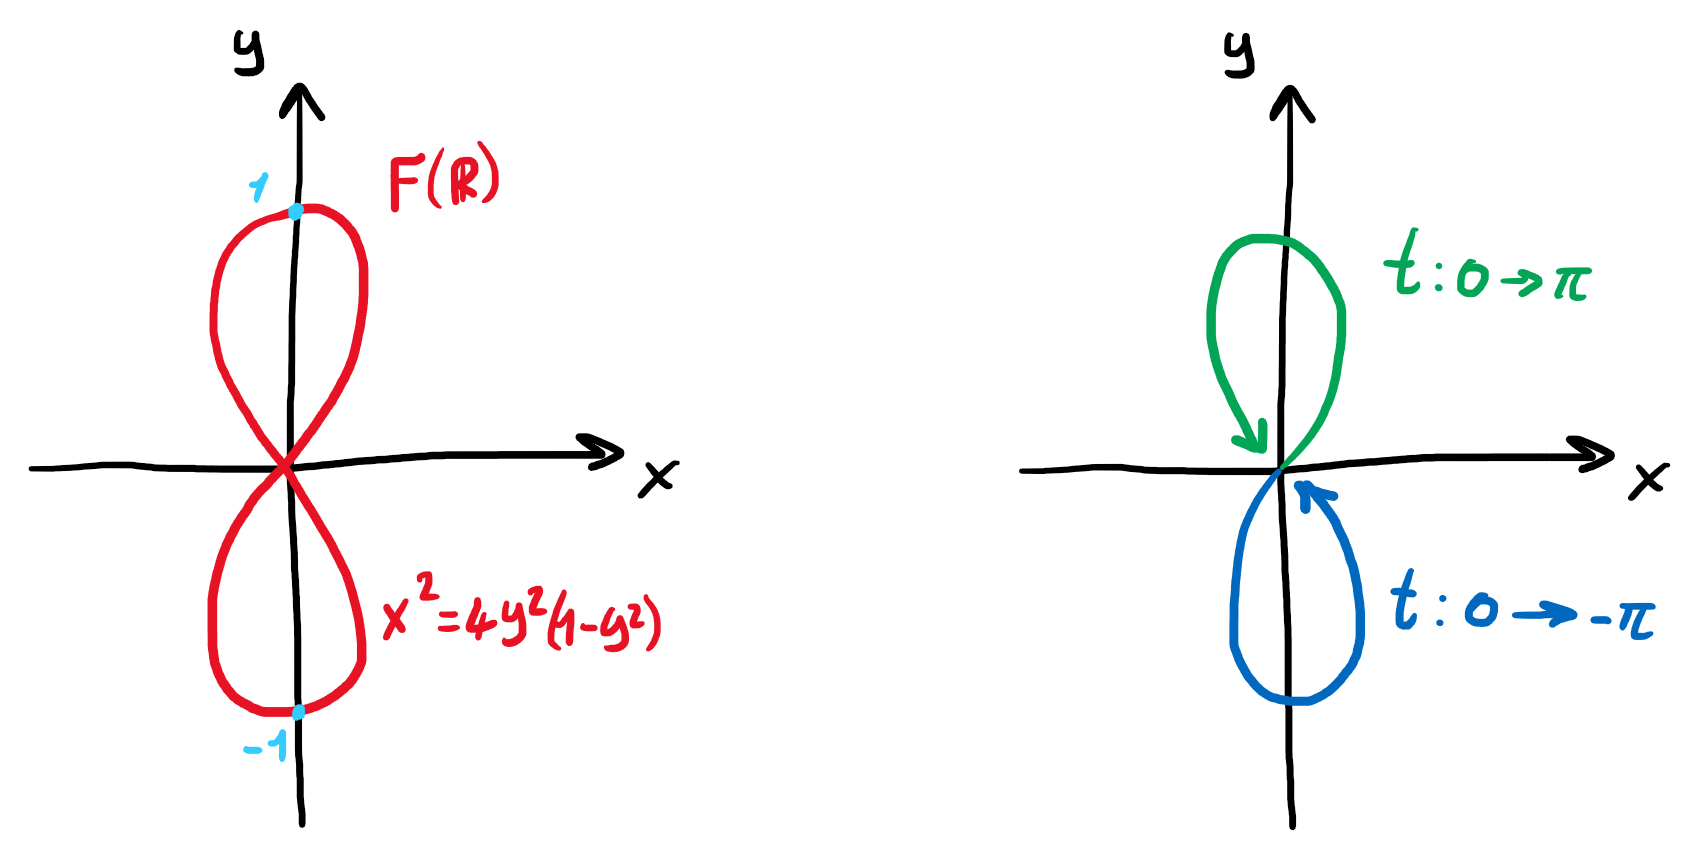
\includegraphics[width=0.7\textwidth,keepaspectratio]{img40}
\end{figure}

Questa è iniettiva perché per due punti dell'immagine uguali $ (\sin(2t_{1}),\sin(t_{1})) = (\sin(2t_{2}),\sin(2t_{2})) $ otteniamo che

\begin{equation}
	\sin(t_{1}) = \sin(t_{2}) = 0 \implies t_{1} = t_{2} = 0 \because t \in (-\pi,\pi)
\end{equation}

oppure $ \sin(t_{1}) = \sin(t_{2}) \neq 0 $ il che implica

\begin{align}
	\begin{split}
		\sin(2t_{1}) &= \sin(2t_{2})\\
		2 \sin(t_{1}) \cos(t_{1}) &= 2 \sin(t_{2}) \cos(t_{2})\\
		\cos(t_{1}) &= \cos(t_{2})
	\end{split}		
\end{align}

perciò

\begin{equation}
	\begin{cases}
		\sin(t_{1}) = \sin(t_{2})\\
		\cos(t_{1}) = \cos(t_{2})
	\end{cases}%
	\implies%
	\begin{aligned}
		t_{1} = t_{2} &+ 2 k \pi\\
		\forall k &\in \Z
	\end{aligned}
	\implies%
	t_{1} = t_{2}
\end{equation}

in quanto qualsiasi valore di $ k $ diverso da 0 esce dall'intervallo del dominio.\\
Questa applicazione è un'immersione in quanto

\begin{equation}
	\dot{F}(t) = (2 \cos(2t), \cos(t)) \neq (0,0), \qquad \forall t \in \R
\end{equation}

Nonostante sia un'immersione iniettiva, non è un embedding (né topologico né differenziabile) in quanto $ F((-\pi,\pi)) $ non è localmente euclidea nell'origine.

\paragraph{5)}

Sia l'applicazione

\begin{align}
	\begin{split}
		F : \R &\to \S^{1} \times \S^{1} = \T^{2}\\
		t &\mapsto (x,y) = (e^{2 \pi i t}, e^{2 \pi i \alpha t})
	\end{split}
\end{align}

dove $ \alpha \in \R \setminus \Q $ ($ \alpha $ irrazionale); siccome il toro $ \T^{2} $ è incluso in $ \R^{4} $, possiamo riscrivere la funzione come

\begin{align}
	\begin{split}
		F : \R &\to \R^{4}\\
		t &\mapsto (x,y) = (\cos(2 \pi t), \sin(2 \pi t), \cos(2 \pi \alpha t), \sin(2 \pi \alpha t))
	\end{split}
\end{align}

in quanto abbiamo considerato $ \S^{1} \subset \R^{2} = \C $.\\
Verifichiamo se $ F $ sia iniettiva tramite la dimostrazione dell'implicazione

\begin{equation}
	\begin{cases}
		e^{2 \pi i t_{1}} = e^{2 \pi i t_{2}}\\
		e^{2 \pi i \alpha t_{1}} = e^{2 \pi i \alpha t_{2}}
	\end{cases}%
	\implies%
	t_{1} = t_{2}
\end{equation}

Quindi possiamo scrivere

\begin{equation}
	\begin{cases}
		e^{2 \pi i t_{1}} = e^{2 \pi i t_{2}}\\
		e^{2 \pi i \alpha t_{1}} = e^{2 \pi i \alpha t_{2}}
	\end{cases}%
	\implies%
	\begin{cases}
		t_{1} - t_{2} = m & m \in \Z\\
		t_{1} - t_{2} = \alpha n & \alpha,n \in \Z
	\end{cases}%
	\implies%
	\alpha n = m%
	\implies%
	\alpha \in \Q
\end{equation}

ma questo non è possibile in quanto abbiamo posto $ \alpha \in \R \setminus \Q $, dunque l'applicazione è iniettiva.\\
Per verificare se sia un'immersione, consideriamo la derivata di $ F $ in $ \R^{4} $

\begin{equation}
	\dot{F}(t) = (- 2 \pi \sin(2 \pi t), 2 \pi \cos(2 \pi t), - 2 \pi \alpha \sin(2 \pi \alpha t), 2 \pi \alpha \cos(2 \pi \alpha t))
\end{equation}

la quale non si annulla per $ \forall t \in \R $.\\
Nonostante $ F $ sia un'immersione iniettiva, questa non è un embedding in quanto la sua immagine non è una sottovarietà di $ \R^{4} $.\\
Dimostriamo questo fatto mediante il seguente lemma


\begin{lemma}
	Chiamando $ \mathcal{D}(A) $ l'insieme dei punti di accumulazione\footnote{%
		Per un punto di accumulazione di un insieme, ogni intorno di questo punto contiene un punto dell'insieme diverso da sé stesso.%
	} di un insieme $ A $, possiamo affermare che
	
	\begin{equation}
		F(0) = (1,1) \in \mathcal{D}(F(\Z))
	\end{equation}

	Cioè qualunque intorno di $ (1,1) \in \T^{2} $ include almeno un punto di $ F(\Z) $ o equivalentemente
	
	\begin{equation}
		\forall \varepsilon > 0, \, \E k \in \Z \setminus 0 \mid \left| (e^{2 \pi i k}, e^{2 \pi i \alpha k}) - (1,1) \right| < \varepsilon
	\end{equation}
\end{lemma}

\begin{proof}
	\begin{align}
		\begin{split}
			\left| (e^{2 \pi i k}, e^{2 \pi i \alpha k}) - (1,1) \right| &< \varepsilon\\
			\left| (1, e^{2 \pi i \alpha k}) - (1,1) \right| &< \varepsilon\\
			\left| e^{2 \pi i \alpha k} - 1 \right| &< \varepsilon
		\end{split}
	\end{align}

	Sappiamo che $ \S^{1} $ è compatto quindi la successione di punti del cerchio
	
	\begin{equation}
		z_{n} = e^{2 \pi i \alpha k}, \qquad n \in \Z
	\end{equation}

	ammette una sottosuccessione convergente: possiamo supporre che (a meno di cambiare semplicemente gli indici della successione) la successione stessa converga a un punto $ z_{n} \to z_{0} \in \S^{1} $ e ciò significa che esistono due numeri (diversi) $ n_{1},n_{2} \in \Z $ tali che si possa scrivere
	
	\begin{equation}
		\left| e^{2 \pi i \alpha n_{1}} - 1 \right| < \dfrac{\varepsilon}{2} \quad \wedge \quad \left| e^{2 \pi i \alpha n_{2}} - 1 \right| < \dfrac{\varepsilon}{2}
	\end{equation}

	ponendo dunque $ k = n_{1} - n_{2} \neq 0 $ e sfruttando la diseguaglianza triangolare
	
	\begin{align}
		\begin{split}
			\left| e^{2 \pi i \alpha k} - 1 \right| &= \left| e^{2 \pi i \alpha (n_{1} - n_{2})} - 1 \right|\\
			&= \left| e^{ -2 \pi i \alpha n_{2}} \left( e^{2 \pi i \alpha n_{1}} - e^{2 \pi i \alpha n_{2}} \right) \right|\\
			&= \left| e^{ -2 \pi i \alpha n_{2}} \right| \left| e^{2 \pi i \alpha n_{1}} - e^{2 \pi i \alpha n_{2}} \right|\\
			&= \left| e^{2 \pi i \alpha n_{1}} - e^{2 \pi i \alpha n_{2}} \right|\\
			&= \left| e^{2 \pi i \alpha n_{1}} - e^{2 \pi i \alpha n_{2}} +1 -1 \right|\\
			&\leqslant \left| e^{2 \pi i \alpha n_{1}} - 1 \right| + \left| e^{2 \pi i \alpha n_{2}} - 1 \right|\\
			&= \sfrac{\varepsilon}{2} + \sfrac{\varepsilon}{2}\\
			&= \varepsilon
		\end{split}
	\end{align}

	dunque
	
	\begin{equation}
		\left| e^{2 \pi i \alpha k} - 1 \right| < \varepsilon
	\end{equation}
\end{proof}

Supponiamo per assurdo che $ F $ sia un embedding: l'applicazione $ f : \R \to F(\R) $ con la topologia di $ F(\R) $ indotta dal toro $ \T^{2} $ è un diffeomorfismo e dunque anche un omeomorfismo. Per le proprietà degli omeomorfismi, esiste una bigezione tra i punti di accumulazione del dominio e quelli del codominio, i.e. $ \mathcal{D}(\Z) \to \mathcal{D}(F(\Z)) $, però $ \mathcal{D}(\Z) = \emptyset $ in quanto i numeri interi sono isolati in $ \R $ mentre $ \mathcal{D}(F(\Z)) \ni (1,1) $. Questa contraddizione porta a dire che $ F $ non è un embedding e quindi $ F(\R) $ non è una sottovarietà di $ \T^{2} $.

\begin{remark}
	Si dimostra che $ F(\R) $ è denso in $ \T^{2} $, cioè il toro è completamente ricoperto dall'immagine della funzione o equivalentemente ogni intorno di ogni punto del toro ha al suo interno un punto dell'immagine (per dimostrare questo, viene utilizzata la teoria dei numeri).
\end{remark}

\subsubsection{Immagini di applicazioni lisce contenute in varietà}

\begin{theorem}
	Siano $ F : N \to M $ un'applicazione liscia tra varietà e $ S \subset M $ una sottovarietà di $ M $ e supponiamo che $ F(N) \subseteq S $, allora la restrizione del codominio della funzione al sottoinsieme $ S $ è ancora un'applicazione liscia, i.e. $ \tilde{F} : N \to S $ con $ \tilde{F}(q) = F(q) $ per $ \forall q \in N $.
\end{theorem}

\begin{proof}
	Sappiamo che $ \tilde{F} $ è continua in quanto $ S $ è un sottospazio topologico di $ M $.\\
	Siano $ p \in N $ un punto e due carte $ (U,\phi) \in N $ intorno a $ p $ con $ \phi = (x^{1},\dots,x^{n}) $ e $ (V,\psi) \in M $ intorno a $ F(p) $ con $ \psi = (y^{1},\dots,y^{m}) $ tali che $ F(U) \subseteq V $ e tale che $ (V,\psi) $ sia una carta adattata intorno a $ F(p) $ relativamente a $ S $.\\
	Se $ \dim(S)=s $, possiamo scrivere la condizione per le sottovarietà
	
	\begin{equation}
		V \cap S = \{ q \in V \mid y^{s+1}(q) = \cdots = y^{m}(q) = 0 \}
	\end{equation}

	e la restrizione dell'applicazione della carta adattata
	
	\begin{align}
		\begin{split}
			\psi_{|V \cap S} = \psi_{S} : V \cap S &\to \psi(V \cap S) \subset \R^{s}\\
			q &\mapsto (y^{1}(q),\dots,y^{s}(q))
		\end{split}
	\end{align}

	Osserviamo che, dalle carte, $ F(U) \subseteq V $ e che, dalle ipotesi, $ F(N) \subseteq S $ da cui $ F(U) \subseteq S $ perciò $ F(U) \subseteq V \cap S $. Consideriamo la composizione
	
	\begin{align}
		\begin{split}
			\psi \circ F : U &\to V \subset \R^{m}\\
			q &\mapsto ( \, y^{1}(F(q)), \dots, y^{s}(F(q)), 0,\dots, 0 \, )
		\end{split}
	\end{align}

	e poi la restrizione a $ S $
	
	\begin{align}
		\begin{split}
			\psi_{S} \circ \tilde{F} : U &\to V \cap S\\
			q &\mapsto ( \, y^{1}(F(q)), \dots, y^{s}(F(q)) \, )
		\end{split}
	\end{align}

	Siccome le $ y^{i} $, $ F $ e $ \psi_{S} $ sono tutte applicazioni lisce rispetto a $ q $, anche la composizione $ \psi_{S} \circ \tilde{F} $ sarà liscia, il che implica che la restrizione $ \tilde{F} $ è liscia.
\end{proof}

\subsubsection{\textit{Esempi}}

\paragraph{1) Lemniscata di Bernoulli}

Consideriamo le seguenti due varianti della lemniscata di Bernoulli tramite le applicazioni lisce

\begin{align}
	\begin{split}
		F : (-\pi,\pi) &\to \R^{2}\\
		t &\mapsto (\sin(2t),\sin(t))\\\\
		%
		G : (-\pi,\pi) &\to \R^{2}\\
		t &\mapsto (\sin(2t),-\sin(t))
	\end{split}
\end{align}

e chiamiamo le loro immagini $ F((-\pi,\pi)) = \mathfrak{8}_{F} $ e $ G((-\pi,\pi)) = \mathfrak{8}_{G} $, le quali sono varietà differenziabili la cui struttura è indotta rispettivamente da $ F $ o da $ G $ (bigezioni), ma non sono sottovarietà di $ \R^{2} $. Le funzioni che hanno lo stesso dominio e come codominio le immagini del dominio sono diffeomorfismi, i.e.

\begin{align}
	\begin{split}
		\tilde{F} : (-\pi,\pi) &\to \mathfrak{8}_{F}\\
		t &\mapsto (\sin(2t),\sin(t))\\\\
		%
		\tilde{G} : (-\pi,\pi) &\to \mathfrak{8}_{G}\\
		t &\mapsto (\sin(2t),-\sin(t))
	\end{split}
\end{align}

\begin{figure}[H]
	\centering
	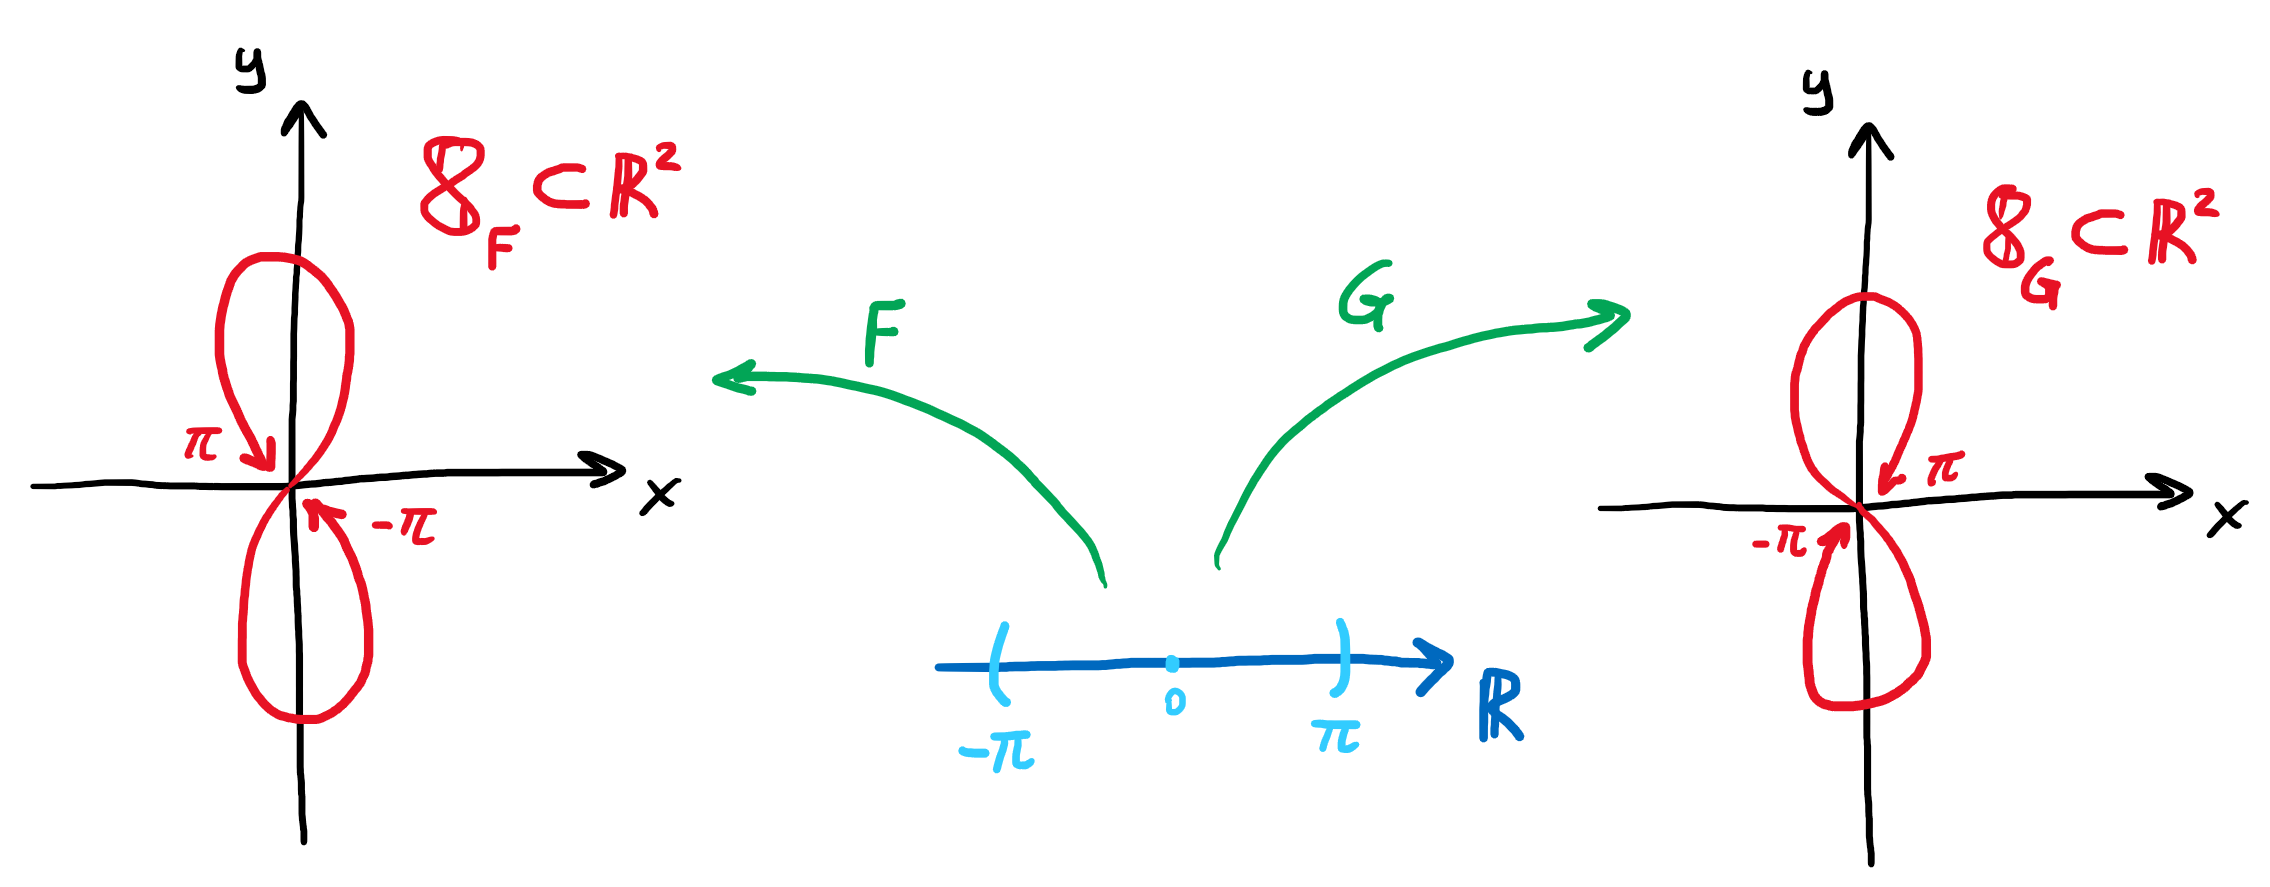
\includegraphics[width=0.8\textwidth,keepaspectratio]{img41}
\end{figure}

Consideriamo ora l'applicazione $ H $ che mappa i punti come $ G $ ma nell'immagine di $ F $, i.e.

\begin{align}
	\begin{split}
		H : (-\pi,\pi) &\to \mathfrak{8}_{F}\\
		t &\mapsto (\sin(2t),-\sin(t))
	\end{split}
\end{align}

il cui codominio possiede la struttura differenziabile indotta da $ G $. Nonostante la funzione $ G $ sia liscia e l'immagine di $ H $ sia contenuta in $ \R^{2} $, $ \mathfrak{8}_{F} $ non è una sottovarietà di $ \R^{2} $ e $ H $ non è nemmeno continua (perciò non liscia): per dimostrarlo è necessario considerare un aperto nel codominio e dimostrare che la sua controimmagine non è aperta nel dominio. Consideriamo dunque l'aperto (segmento) $ U = (a,b) \in \mathfrak{8}_{F} $: la sua controimmagine tramite $ F $ è aperta in $ (-\pi,\pi) $, mentre non è aperta se si prende la sua controimmagine tramite $ H $, i.e.

\begin{equation}
	U = (a,b) \in \mathfrak{8}_{F}%
	\rightarrow%
	\begin{cases}
		F^{-1}(U) = (F^{-1}(a),F^{-1}(b)) & \text{aperta}\\
		H^{-1}(U) = (-\pi,H^{-1}(a)) \cup 0 \cup (H^{-1}(b),\pi) & \text{non aperta}
	\end{cases}
\end{equation}

Il fatto che immagine e preimmagine non siano entrambe aperte rende $ H $ non continua.

\begin{figure}[H]
	\centering
	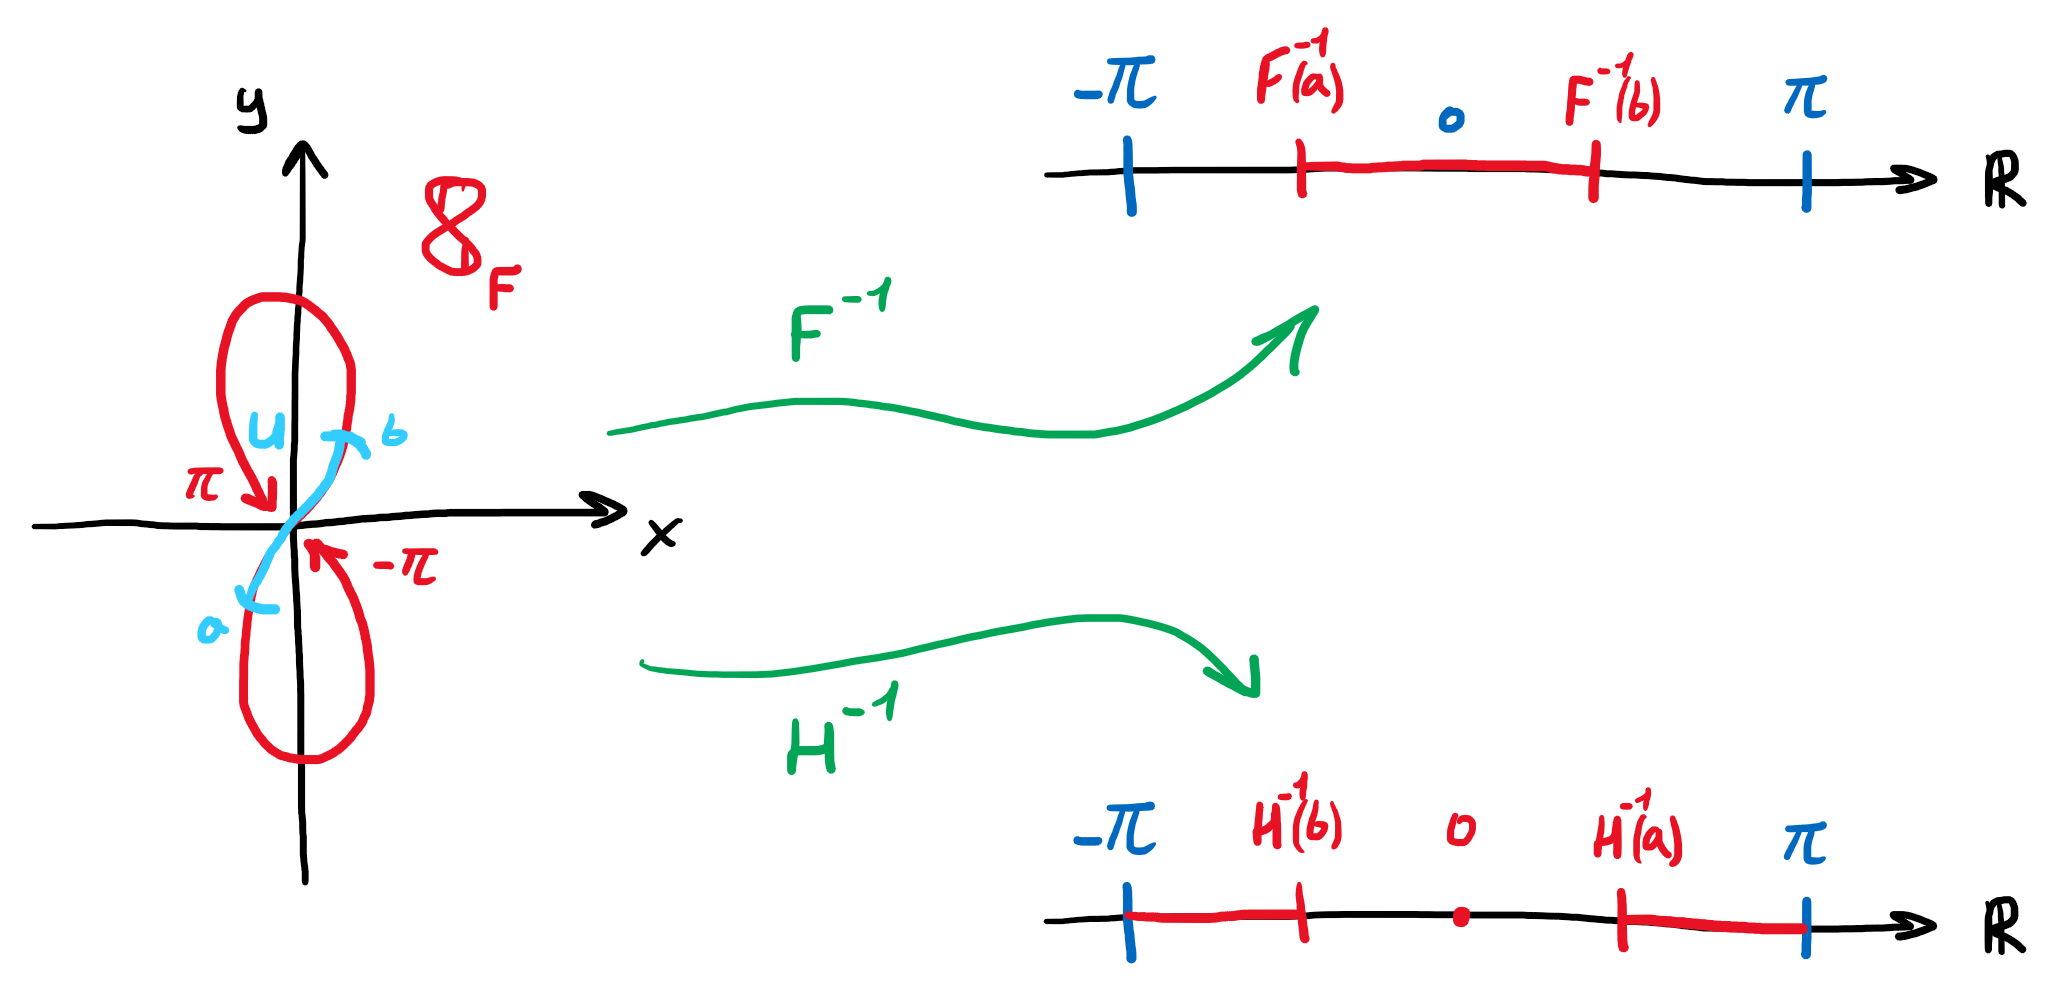
\includegraphics[width=0.8\textwidth,keepaspectratio]{img42}
\end{figure}

Questo esempio mostra come, presa una funzione liscia tra varietà differenziabili, la restrizione del codominio da una varietà a un sottoinsieme (varietà) di questa varietà non è ancora una funzione liscia, a meno che il sottoinsieme della varietà non sia una sottovarietà di questa (quindi con la relativa struttura ereditata): in questo caso, restringere il codominio $ \R^{2} $ della funzione $ G $ alla varietà $ \mathfrak{8}_{F} \subset \R^{2} $ (la quale non è una sottovarietà di $ \R^{2} $) non rende la funzione $ H $ nemmeno continua. Quest'ultimo risultato può essere derivato anche dal fatto che la lemniscata di Bernoulli non sia un sottospazio topologico di $ \R^{2} $.

\paragraph{2) Gruppo lineare speciale}\label{ex-slnr}

Sia l'insieme

\begin{equation}
	SL_{n}(\R) = \{ A \in GL_{n}(\R) \mid \det(A)=1 \} \subset GL_{n}(\R)
\end{equation}

il quale è una sottovarietà di $ GL_{n}(\R) $.\\
Consideriamo l'applicazione del prodotto tra matrici di $ SL_{n}(\R) $

\begin{align}
	\begin{split}
		\mu : SL_{n}(\R) \times SL_{n}(\R) &\to SL_{n}(\R)\\
		(A,B) &\mapsto A B
	\end{split}
\end{align}

e verifichiamo che $ \mu $ sia liscia.\\
Moltiplicare due matrici di $ SL_{n}(\R) $ non è banale, lo sarebbe in $ GL_{n}(\R) $ che ha le carte con gli omeomorfismi verso $ \R^{n^{2}} $, rendendo dunque il prodotto tra matrici una semplice concatenazione di somme e prodotti tra numeri reali.\\
Sia l'applicazione liscia del prodotto tra matrici di $ GL_{n}(\R) $

\begin{align}
	\begin{split}
		F : GL_{n}(\R) \times GL_{n}(\R) &\to GL_{n}(\R)\\
		(A,B) &\mapsto A B
	\end{split}
\end{align}

se restringiamo il dominio a $ SL_{n}(\R) \times SL_{n}(\R) $, otteniamo l'applicazione

\begin{align}
	\begin{split}
		G : SL_{n}(\R) \times SL_{n}(\R) &\to GL_{n}(\R)\\
		(A,B) &\mapsto A B
	\end{split}
\end{align}

definita come $ G = F \circ (i \times i) $ dove $ i : SL_{n}(\R) \to GL_{n}(\R) $ indica l'inclusione: essendo $ F $ e $ i $ lisce (e dunque anche $ i \times i $\footnote{%
	Vedi Esercizio \ref{es2-12}.%
}), anche $ G $ è liscia.\\
Siccome la moltiplicazione di due matrici con determinante unitario è ancora una matrice con determinante unitario, abbiamo che $ G(SL_{n}(\R) \times SL_{n}(\R)) \subset SL_{n}(\R) $ e quindi possiamo restringere il codominio, ottenendo la funzione

\begin{align}
	\begin{split}
		\tilde{G} : SL_{n}(\R) \times SL_{n}(\R) &\to SL_{n}(\R)\\
		(A,B) &\mapsto A B
	\end{split}
\end{align}

la quale è ancora liscia dal teorema. Dalle definizioni, sappiamo che $ \mu \equiv \tilde{G} $ perciò $ \mu $ è liscia.

\section{Il fibrato tangente e i campi di vettori}

\subsection{Fibrato tangente}

Sia $ M $ una varietà differenziabile di dimensione $ n $. Il \textit{fibrato tangente a} $ M $ è definito come l'unione disgiunta di tutti gli spazi tangenti ai punti di $ M $, i.e.

\begin{equation}
	T(M) \doteq \bigsqcup_{p \in M} T_{p}(M)
\end{equation}

La proiezione naturale è definita come

\begin{align}
	\begin{split}
		\pi : T(M) &\to M\\
		v &\mapsto p
	\end{split}
\end{align}

dove notazioni alternative per $ v \in T_{p}(M) $ sono $ (p,v) $ (per evidenziare il collegamento con il punto $ p \in M $) e $ X_{p} $.\\
Costruiamo ora una struttura differenziabile sul fibrato tangente in modo tale da rendere liscia la proiezione.

\subsubsection{Struttura topologica sul fibrato tangente}

Siano $ U \subset M $ un aperto coordinato, i.e. abbiamo fissato una carta $ (U,\phi) \in M $ intorno a $ p $ con $ \phi = (x^{1},\dots,x^{n}) $, e $ T(U) $ il fibrato tangente a $ U $, dunque

\begin{equation}
	T(U) = \bigsqcup_{p \in M} T_{p}(U) = \bigsqcup_{p \in M} T_{p}(M)
\end{equation}

questo perché $ T_{p}(U) = \der_{p}(C_{p}^{\infty}(U)) $ ma siccome il concetto di germe di funzione è locale

\begin{equation}
	T_{p}(U) = \der_{p}(C_{p}^{\infty}(U)) = \der_{p}(C_{p}^{\infty}(M)) = T_{p}(M)
\end{equation}

Esiste una bigezione naturale tra $ T(U) $ a $ \R^{2n} $: prendendo $ v \in T_{p}(M) $ e sapendo che $ \langle \sfrac{\partial}{\partial x^{i}} |_{p} \rangle = T_{p}(M) $, possiamo scrivere

\begin{equation}
	v = \sum_{i=1}^{n} c^{i}(v) \left. \dfrac{\partial}{\partial x^{i}} \right|_{p}
\end{equation}

e chiamiamo $ c(v) = (c^{1}(v),\dots,c^{n}(v)) $; a questo punto, la bigezione può essere scritta come

\begin{align}
	\begin{split}
		\tilde{\phi} : T(U) &\to \phi(U) \times \R^{n} = \R^{2n}\\
		v &\mapsto (\phi(p),c(v))\\
		&\mapsto (x^{1}(p),\dots,x^{n}(p),c^{1}(v),\dots,c^{n}(v))
	\end{split}
\end{align}

dove $ \phi(U) \subset \R^{n} $. Per poter scrivere l'immagine in funzione di solo $ v $, consideriamo l'applicazione

\begin{align}
	\begin{split}
		\phi_{*} = \phi_{*p} : T_{p}(U) &\to T_{\phi(p)}(\phi(U)) =  T_{\phi(p)}(\R^{n})\\
		\left. \dfrac{\partial}{\partial x^{i}} \right|_{p} &\mapsto \left. \dfrac{\partial}{\partial r^{i}} \right|_{p}
	\end{split}
\end{align}

che applicata a $ v $

\begin{align}
	\begin{split}
		\phi_{*}(v) &= \phi_{*} \left( \sum_{i=1}^{n} c^{i}(v) \left. \dfrac{\partial}{\partial x^{i}} \right|_{p} \right)\\
		&= \sum_{i=1}^{n} c^{i}(v) \phi_{*} \left( \left. \dfrac{\partial}{\partial x^{i}} \right|_{p} \right)\\
		&= \sum_{i=1}^{n} c^{i}(v) \left. \dfrac{\partial}{\partial r^{i}} \right|_{p}
	\end{split}
\end{align}

il quale risultato può essere identificato con $ c(v) = (c^{1}(v),\dots,c^{n}(v)) $ in $ \R^{n} $. Da tutto ciò e considerando $ p = \pi(v) $, si può riscrivere $ \tilde{\phi} $ come

\begin{equation}
	\tilde{\phi}(v) = (\phi \circ \pi,\phi_{*})(v) = (\phi(\pi(v)),\phi_{*}(v))
\end{equation}

Questa applicazione è invertibile (essendo una bigezione) e la sua inversa è

\begin{align}
	\begin{split}
		\tilde{\phi}^{-1} : \phi(U) \times \R^{n} &\to T(U)\\
		(\phi(p),c(v)) &\mapsto v = \sum_{i=1}^{n} c^{i}(v) \left. \dfrac{\partial}{\partial x^{i}} \right|_{p}
	\end{split}
\end{align}

Definiamo dunque la topologia su $ T(U) $ (indotta dall'applicazione $ \tilde{\phi} $) come

\begin{equation}
	A \subset T(U) \text{ aperto} \iff \tilde{\phi}(A) \text{ aperto in } \phi(U) \times \R^{n}
\end{equation}

Abbiamo le seguenti conseguenze:

\begin{itemize}
	\item $ \tilde{\phi} : T(U) \to \phi(U) \times \R^{n} $ è un omeomorfismo;
	
	\item Preso $ V \subset U $, la topologia indotta da $ T(U) $ su $ T(V) $ ($ T(V) \subset T(V) $) è la stessa della topologia indotta su $ T(V) $ dall'applicazione $ \tilde{\phi}_{|T(V)} : T(V) \to \phi(V) \times \R^{n} $.
\end{itemize}

Per costruire una topologia su $ T(M) $ consideriamo dunque l'insieme

\begin{equation}
	\mathcal{B}_{T(M)} = \bigcup_{\alpha} \{ A \subset T(U_{\alpha}) \text{ aperti} \}
\end{equation}

cioè l'unione di tutti gli aperti $ A $ contenuti nei rispettivi $ T(U_{\alpha}) $ al variare di $ \alpha $, dove $ U_{\alpha} $ è un aperto coordinato dell'atlante massimale di $ M $.

\begin{definition}
	L'insieme $ \mathcal{B}_{T(M)} $ è una base per una topologia su $ T(M) $.
\end{definition}

\begin{proof}
	Per la dimostrazione è necessario che
	
	\begin{itemize}
		\item $ \mathcal{B}_{T(M)} $ sia un ricoprimento di $ T(M) $;
		
		\item L'intersezione di due elementi di $ \mathcal{B}_{T(M)} $ si può scrivere come unione di elementi di $ \mathcal{B}_{T(M)} $.
	\end{itemize}

	Per definizione $ T(U_{\alpha}) \in \mathcal{B}_{T(M)} $ in quanto aperto; abbiamo anche che vale la seguente implicazione
	
	\begin{equation}
		\bigcup_{\alpha} U_{\alpha} = M \implies \bigcup_{\alpha} T(U_{\alpha}) = T(M)
	\end{equation}

	perciò $ \mathcal{B}_{T(M)} $ è un ricoprimento di $ T(M) $.\\
	Siano due aperti $ A \subset T(U) $ e $ B \subset T(V) $, i.e. $ A,B \in \mathcal{B}_{T(M)} $, con $ U $ e $ V $ due aperti coordinati (i.e. fanno parte di carte di $ T(U) $ e $ T(V) $ rispettivamente). Dimostrando che $ T(U) \cap T(V) = T(U \cap V) $ tramite
	
	\begin{align}
		\begin{split}
			T(U) \cap T(V) &= \left( \bigsqcup_{p \in U} T_{p}(U) \right) \cap \left( \bigsqcup_{q \in V} T_{p}(V) \right)\\
			&= \left( \bigsqcup_{p \in U} T_{p}(M) \right) \cap \left( \bigsqcup_{q \in V} T_{p}(M) \right)\\
			&= \bigsqcup_{r \in U \cap V} T_{r}(M)\\
			&= \bigsqcup_{r \in U \cap V} T_{r}(U \cap V)\\
			&= T(U \cap V)
		\end{split}
	\end{align}
	
	possiamo scrivere che
	
	\begin{equation}
		A \cap B \subset T(U) \cap T(V) = T(U \cap V)
	\end{equation}

	dove $ U \cap V $ è ancora un aperto coordinato della carta $ (U \cap V,\phi_{|U \cap V}) $. Dobbiamo verificare ora che $ A \cap B \subset T(U \cap V) $ sia aperto in $ T(U \cap V) $ (l'intersezione di due elementi della base si può scrivere come unione di elementi della base) perché $ \mathcal{B}_{T(M)} $ sia effettivamente una base: osserviamo che
	
	\begin{align}
		\begin{split}
			A \cap B &= (A \cap B) \cap T(U \cap V)\\
			&= (A \cap T(U \cap V)) \cap (B \cap T(U \cap V))
		\end{split}
	\end{align}

	perciò, perché $ A \cap B $ sia aperto in $ T(U \cap V) $, è sufficiente che $ A \cap T(U \cap V) $ sia aperto in $ T(U \cap V) $ (risp. per $ B $). Questo è vero perché $ T(U \cap V) \subset T(U) $ e ha la topologia indotta da $ T(U) $ (perché $ U \cap V \subset U $) e i suoi aperti sono gli aperti di $ T(U) $ (e.g. $ A $) intersecati con $ T(U \cap V) $ stesso, i.e. $ A \cap T(U \cap V) $; il ragionamento è analogo per $ B $.
\end{proof}

A questo punto $ T(M) $ è uno spazio topologico con la topologia che ha $ \mathcal{B}_{T(M)} $ come base.\footnote{%
	Questa topologia per $ T(M) $ è l'unica possibile.%
}\\
Dobbiamo far vedere ora che $ T(M) $ è una varietà topologica e per farlo dobbiamo mostrare che sia $ N_{2} $, $ T_{2} $ e localmente euclideo.\\
Useremo il seguente lemma per dimostrare il secondo criterio di numerabilità $ N_{2} $:

\begin{lemma}
	Ogni varietà differenziabile ha una base numerabile di insiemi coordinati o equivalentemente esiste un atlante differenziabile numerabile.
\end{lemma}

\begin{proof}
	Siano $ \{(U_{\alpha},\phi_{\alpha})\} $ l'atlante massimale di $ M $ che definisce la struttura differenziabile di $ M $ e $ \mathfrak{U} = \{U_{i}\}_{i \in I} $ una base numerabile per la topologia di $ M $ (questa esiste in quanto $ M $ è $ N_{2} $).\\
	Presi un punto $ p \in M $ e un aperto $ U_{\alpha} $ di una carta dell'atlante, esiste sempre $ B_{p,\alpha} \in \mathfrak{U} $ tale che $ p \in B_{p,\alpha} \subset U_{\alpha} $, in quanto $ \mathfrak{U} $ è una base. Consideriamo ora la famiglia di aperti $ \mathfrak{B} = \{B_{p,\alpha}\} $ senza duplicati, la quale sarà una sottofamiglia di $ \mathfrak{U} $ e, in quanto tale, sarà numerabile perché $ \mathfrak{U} $ è numerabile. Inoltre $ (B_{p,\alpha}, \phi_{|B_{p,\alpha}}) $ è una carta di $ M $ e dunque $ \{(B_{p,\alpha}, \phi_{|B_{p,\alpha}})\} $ è un atlante differenziabile numerabile per $ M $.\\
	Resta da dimostrare che $ \mathfrak{B} $ sia una base (già numerabile) per $ M $: siano $ p \in M $ e $ U \ni p $ aperto di $ M $, siccome esiste sempre un aperto di una carta che sia contenuto in un aperto della varietà, possiamo scrivere $ p \in U_{\alpha} \subset U $, dove la carta considerata dell'atlante è $ (U \cap U_{\alpha},\phi_{U \cap U_{\alpha}}) $; sappiamo anche che esiste $ B_{p,\alpha} $ tale che $ p \in B_{p,\alpha} \subset U_{\alpha} $, dunque $ p \in B_{p,\alpha} \subset U $. Questo significa che esiste sempre un aperto $ B_{p,\alpha} \in \mathfrak{B} $ che si interponga tra ogni punto della varietà e ogni aperto che contiene il punto stesso, i.e. $ \mathfrak{B} $ è una base per $ M $.
\end{proof}

\paragraph{Localmente euclideo}

Sia $ \{(U_{\alpha},\phi_{\alpha})\} $ un atlante topologico per $ M $, allora $ \{(T(U_{\alpha}),\tilde{\phi}_{\alpha})\} $ è un atlante topologico per $ T(M) $. Questo è vero perché i $ T(U_{\alpha}) $ sono un ricoprimento di $ T(M) $, i.e.

\begin{equation}
	\bigcup_{\alpha} T(U_{\alpha}) = T(M)
\end{equation}

e le applicazioni

\begin{equation}
	\tilde{\phi}_{\alpha} : T(U_{\alpha}) \to \phi_{\alpha}(U_{\alpha}) \times \R^{n}
\end{equation}

sono omeomorfismi in aperti di $ \R^{2n} $, dunque $ \dim(T(M)) = 2 \dim(M) = 2n $.

\paragraph{$ T_{2} $ o di Hausdorff}

Per definizione, un insieme è di Hausdorff se, dati due punti, esistono due intorni disgiunti che contengono questi due punti.\\
Siano $ (p,v) \in T_{p}(M) $ e $ (q,w) \in T_{q}(M) $ due punti distinti di $ T(M) $: presi $ v \neq w $, abbiamo due casi

\begin{itemize}
	\item se $ p = q $ allora $ T_{p}(M) = T_{q}(M) \subset T(U) $ dove $ U $ è un aperto coordinato di $ (U,\phi) \ni p=q $, ma $ T(U) \simeq \phi(U) \times \R^{n} $ dunque $ T(U) $ eredita la proprietà $ T_{2} $ da $ \phi(U) \times \R^{n} $ e a sua volta $ T_{p}(M) = T_{q}(M) $ la eredita da $ T(U) $, i.e.
	
	\begin{equation}
		\E A,B \in T(U) = T(M) \text{ aperti}, \, A \ni (p,v) \wedge B \ni (q,w) \mid A \cap B = \emptyset
	\end{equation}
	
	\item se $ p \neq q $, siccome $ M $ è $ T_{2} $ esisteranno due aperti disgiunti coordinati che contengono $ p $ e $ q $, i.e.
	
	\begin{equation}
		\E U,V \in M, \, U \ni p \wedge V \ni q, \, (U,\phi),(V,\psi) \in M \mid U \cap V = \emptyset
	\end{equation}

	per cui, siccome $ T(U) \ni (p,v) $ e $ T(V) \ni (q,w) $ e
	
	\begin{equation}
		T(U) \cap T(V) = T(U \cap V) = \emptyset \quad \because \quad U \cap V = \emptyset
	\end{equation}

	abbiamo che $ T(M) $ è di Hausdorff.
\end{itemize}

\paragraph{$ N_{2} $}

Sia $ \{(U_{i},\phi_{i})\} $ un atlante differenziabile numerabile di $ M $ (la sua esistenza segue dal lemma dimostrato sopra), allora gli omeomorfismi

\begin{equation}
	\tilde{\phi}_{i} : T(U_{i}) \to \phi_{i}(U_{i}) \times \R^{n}
\end{equation}

permettono di dire, siccome $ T(U_{i}) \simeq \phi(U_{i}) \times \R^{n} $ e $ \phi(U_{i}) \times \R^{n} $ è $ N_{2} $, che $ T(U_{i}) $ sia $ N_{2} $.\\
Fissato $ i In I $, sia $ \{B_{ij}\}_{j \in J} $ una base numerabile (con $ I $ e $ J $ numerabili) per $ T(U_{i}) $, allora l'unione

\begin{equation}
	\bigcup_{i \in I, j \in J} \{B_{ij}\}
\end{equation}

è una base numerabile per $ T(M) $ e dunque $ T(M) $ è $ N_{2} $.

\subsubsection{Struttura differenziabile sul fibrato tangente}

Dopo aver dimostrato che $ T(M) $ è una varietà topologica, dimostriamo che è anche una varietà differenziabile con atlante differenziabile $ \{(T(U_{\alpha}),\tilde{\phi}_{\alpha})\}_{\alpha \in A} $ dove $ \{(U_{\alpha},\phi_{\alpha})\}_{\alpha \in A} $ è un atlante differenziabile per $ M $. L'unico fatto da verificare è che le carte siano $ C^{\infty} $-compatibili o equivalentemente che i cambi di carte siano lisci.\\
Considerando che $ U_{\alpha} \cap U_{\beta} = U_{\alpha \beta} $, 

\begin{equation}
	T(U_{\alpha}) \cap T(U_{\beta}) = T(U_{\alpha} \cap U_{\beta}) \doteq T(U_{\alpha \beta})
\end{equation}

possiamo scrivere i cambi di carta come

\begin{align}
	\begin{split}
		\tilde{\phi}_{\beta} \circ \tilde{\phi}_{\alpha}^{-1} : \tilde{\phi}_{\alpha}(T(U_{\alpha \beta})) &\to \tilde{\phi}_{\beta}(T(U_{\alpha \beta}))\\
		\tilde{\phi}_{\alpha} \circ \tilde{\phi}_{\beta}^{-1} : \tilde{\phi}_{\beta}(T(U_{\alpha \beta})) &\to \tilde{\phi}_{\alpha}(T(U_{\alpha \beta}))
	\end{split}
\end{align}

i quali devono essere lisci per $ \forall \alpha,\beta \in A $, dove i $ T(U_{\alpha \beta}) $ sono aperti di $ \R^{2n} $.\\
Scriviamo le singole applicazioni come

\begin{align}
	\begin{split}
		\tilde{\phi}_{\alpha} : T(U_{\alpha}) &\to \phi_{\alpha}(U_{\alpha}) \times \R^{n}\\
		v &\mapsto (\phi_{\alpha} \circ \pi, \phi_{*p})(v)
	\end{split}
\end{align}

dove\footnote{%
Il simbolo $ \longleftrightarrow $ indica l'identificazione.%
}

\begin{equation}
	\begin{cases}
		v = \sum_{i=1}^{n} a^{i}(v) \left. \dfrac{\partial}{\partial x^{i}} \right|_{p}\\
		\pi(v) = p\\
		\phi_{*}(v) = \sum_{i=1}^{n} a^{i}(v) \left. \dfrac{\partial}{\partial r^{i}} \right|_{p} \longleftrightarrow a(v) = (a^{1}(v),\dots,a^{n}(v)) \in \R^{n}
	\end{cases}	
\end{equation}

e la carta utilizzata è $ (U_{\alpha},\phi_{\alpha}) $ con $ \phi_{\alpha} = (x^{1},\dots,x^{n}) $. A questo possiamo riscrivere l'applicazione

\begin{align}
	\begin{split}
		\tilde{\phi}_{\alpha} : T(U_{\alpha}) &\to \phi_{\alpha}(U_{\alpha}) \times \R^{n}\\
		v &\mapsto (\phi_{\alpha} \circ \pi, \phi_{*p})(v)\\
		&\mapsto ( \, x^{1}(\pi(v)),\dots,x^{n}(\pi(v)), a^{1}(v),\dots,a^{n}(v))
	\end{split}
\end{align}

e la sua inversa

\begin{align}
	\begin{split}
		\tilde{\phi}_{\alpha}^{-1} : \phi_{\alpha}(U_{\alpha}) \times \R^{n} &\to T(U_{\alpha})\\
		(\phi_{\alpha}(p), a^{1},\dots,a^{n}) &\mapsto \sum_{i=1}^{n} a^{i}(v) \left. \dfrac{\partial}{\partial x^{i}} \right|_{p}
	\end{split}
\end{align}

Per la funzione $ \tilde{\phi}_{\beta} $ usiamo la carta $ (U_{\beta},\phi_{\beta}) $ con $ \phi_{\beta} = (y^{1},\dots,y^{n}) $ e

\begin{equation}
	\begin{cases}
		v = \sum_{i=1}^{n} b^{i}(v) \left. \dfrac{\partial}{\partial y^{i}} \right|_{p}\\
		\pi(v) = p\\
		\phi_{*}(v) = \sum_{i=1}^{n} b^{i}(v) \left. \dfrac{\partial}{\partial r^{i}} \right|_{p} \longleftrightarrow b(v) = (b^{1}(v),\dots,b^{n}(v)) \in \R^{n}
	\end{cases}	
\end{equation}

da cui

\begin{align}
	\begin{split}
		\tilde{\phi}_{\beta} : T(U_{\beta}) &\to \phi_{\beta}(U_{\beta}) \times \R^{n}\\
		v &\mapsto (\phi_{\beta} \circ \pi, \phi_{*p})(v)\\
		&\mapsto ( \, y^{1}(\pi(v)),\dots,y^{n}(\pi(v)), b^{1}(v),\dots,b^{n}(v))\\\\
		%
		\tilde{\phi}_{\beta}^{-1} : \phi_{\beta}(U_{\beta}) \times \R^{n} &\to T(U_{\beta})\\
		(\phi_{\beta}(p), b^{1},\dots,b^{n}) &\mapsto \sum_{i=1}^{n} b^{i}(v) \left. \dfrac{\partial}{\partial y^{i}} \right|_{p}
	\end{split}
\end{align}

In $ T(U_{\alpha \beta}) $, il vettore $ v $ può essere scritto nei seguenti due modi

\begin{equation}
	v = \sum_{j=1}^{n} a^{j}(v) \left. \dfrac{\partial}{\partial x^{j}} \right|_{p} = \sum_{k=1}^{n} b^{k}(v) \left. \dfrac{\partial}{\partial y^{k}} \right|_{p}
\end{equation}

da cui otteniamo

\begin{align}
	\begin{split}
		v(y^{i}) &= \sum_{j=1}^{n} a^{j}(v) \, \dfrac{\partial y^{i}}{\partial x^{j}} (p)\\
		&= \sum_{k=1}^{n} b^{k}(v) \, \dfrac{\partial y^{i}}{\partial y^{k}} (p)\\
		&= \sum_{k=1}^{n} b^{k}(v) \, \delta^{ik}\\
		&= b^{i}(v)\\\\
		%
		v(x^{i}) &= \sum_{k=1}^{n} b^{k}(v) \, \dfrac{\partial x^{i}}{\partial y^{k}} (p)\\
		&= \sum_{j=1}^{n} a^{j}(v) \, \dfrac{\partial x^{i}}{\partial x^{j}} (p)\\
		&= \sum_{k=1}^{n} a^{j}(v) \, \delta^{ij}\\
		&= a^{i}(v)
	\end{split}
\end{align}

perciò

\begin{align}
	\begin{split}
		b^{i}(v) &= \sum_{k=1}^{n} a^{k}(v) \, \dfrac{\partial y^{i}}{\partial x^{k}} (p)\\
		%
		a^{i}(v) &= \sum_{k=1}^{n} b^{k}(v) \, \dfrac{\partial x^{i}}{\partial y^{k}} (p)
	\end{split}
\end{align}

Possiamo dunque scrivere i cambi di carte

\begin{align}
	\begin{split}
		(\tilde{\phi}_{\beta} \circ \tilde{\phi}_{\alpha}^{-1}) (\phi_{\alpha}(p), a^{1},\dots,a^{n}) &= \tilde{\phi}_{\beta} \left( p, \sum_{i=1}^{n} a^{i}(v) \left. \dfrac{\partial}{\partial x^{i}} \right|_{p} \right)\\
		&= \tilde{\phi}_{\beta} \left( p, v = \sum_{i=1}^{n} a^{i}(v) \left. \dfrac{\partial}{\partial x^{i}} \right|_{p} \right)\\
		&= ( \phi_{\beta}(p), b^{1}(v),\dots,b^{n}(v) )\\
		&= \left( (\phi_{\beta} \circ \phi_{\alpha}^{-1})(\phi_{\alpha}(p)), \sum_{i=1}^{n} a^{k}(v) \, \dfrac{\partial y^{1}}{\partial x^{k}} (p) ,\dots, \sum_{i=1}^{n} a^{k}(v) \, \dfrac{\partial y^{n}}{\partial x^{k}} (p) \right)
	\end{split}
\end{align}

ricordando che le entrate della matrice jacobiana sono equivalenti a

\begin{equation}
	\dfrac{\partial y^{j}}{\partial x^{k}} (p) = \dfrac{\partial (\phi_{\beta} \circ \phi_{\alpha}^{-1})^{j}}{\partial r^{k}} (\phi(p))
\end{equation}

otteniamo, applicando un ragionamento analogo per il cambio di carte inverso, le seguenti uguaglianze

\begin{multline}
	(\tilde{\phi}_{\beta} \circ \tilde{\phi}_{\alpha}^{-1}) (\phi_{\alpha}(p), a^{1},\dots,a^{n}) =\\
	= \left( (\phi_{\beta} \circ \phi_{\alpha}^{-1})(\phi_{\alpha}(p)), \sum_{i=1}^{n} a^{k}(v) \, \dfrac{\partial (\phi_{\beta} \circ \phi_{\alpha}^{-1})^{1}}{\partial r^{k}} (\phi_{\alpha}(p)) ,\dots, \sum_{i=1}^{n} a^{k}(v) \, \dfrac{\partial (\phi_{\beta} \circ \phi_{\alpha}^{-1})^{n}}{\partial r^{k}} (\phi_{\alpha}(p)) \right)
\end{multline}

\begin{multline}
	(\tilde{\phi}_{\alpha} \circ \tilde{\phi}_{\beta}^{-1}) (\phi_{\beta}(p), b^{1},\dots,b^{n}) =\\
	= \left( (\phi_{\alpha} \circ \phi_{\beta}^{-1})(\phi_{\beta}(p)), \sum_{i=1}^{n} b^{k}(v) \, \dfrac{\partial (\phi_{\alpha} \circ \phi_{\beta}^{-1})^{1}}{\partial r^{k}} (\phi_{\beta}(p)) ,\dots, \sum_{i=1}^{n} b^{k}(v) \, \dfrac{\partial (\phi_{\alpha} \circ \phi_{\beta}^{-1})^{n}}{\partial r^{k}} (\phi_{\beta}(p)) \right)
\end{multline}

Questi cambi di carte sono lisci perché

\begin{itemize}
	\item per le prime $ n $ componenti $ (\phi_{\alpha} \circ \phi_{\beta}^{-1})(\phi_{\beta}(p)) $: $ \phi_{\beta} \circ \phi_{\alpha}^{-1} $ e $ \phi_{\alpha} \circ \phi_{\beta}^{-1} $ sono i cambi di carte in $ M $ tra $ (U_{\alpha},\phi_{\alpha}) $ e $ (U_{\beta},\phi_{\beta}) $;
	
	\item per le seconde $ n $ componenti: le derivate parziali dei cambi di carte applicate ai punti $ \phi_{\alpha}(p) $ e $ \phi_{\beta}(p) $ moltiplicate per numeri reali $ a^{i} $ e $ b^{i} $ e sommate tra loro sono ancora lisce
\end{itemize}

Questo mostra che $ T(M) $ è una varietà differenziabile di dimensione $ 2n $.

\subsubsection{Proiezione dal fibrato tangente}

Dimostriamo ora che la proiezione dal fibrato tangente di una varietà alla varietà stessa, i.e.

\begin{align}
	\begin{split}
		\pi : T(M) &\to M\\
		(p,v) &\mapsto p
	\end{split}
\end{align}

è liscia: per mostrarlo, prendiamo due carte arbitrarie e facciamo vedere che l'espressione locale è liscia.\\
Siano le carte $ (U,\phi) \in M $ intorno a $ p $ con $ \phi = (x^{1},\dots,x^{n}) $ e $ (T(U),\tilde{\phi}) \in T(M) $ intorno a $ (p,v) \in T_{p}(M) $, dove

\begin{equation}
	v = \sum_{i=1}^{n} c^{i}(v) \left. \dfrac{\partial}{\partial x^{i}} \right|_{p}
\end{equation}

con $ c(v) = (c^{1}(v),\dots,c^{n}(v)) $. Ricordando l'applicazione $ \tilde{\phi} $

\begin{equation}
	\tilde{\phi}(p,v) = (\phi(p),c(v)) = (x^{1}(p),\dots,x^{n}(p),c^{1}(v),\dots,c^{n}(v))
\end{equation}

abbiamo che

\begin{equation}
	(\phi \circ \pi \circ \tilde{\phi}^{-1}) (\phi(p),c^{1},\dots,c^{n}) = (\phi \circ \pi) \left( p, \sum_{i=1}^{n} c^{i} \left. \dfrac{\partial}{\partial x^{i}} \right|_{p} \right) = \phi(p)
\end{equation}

dunque $ \pi $ è localmente liscia (e anche lineare) in quanto proiezione sulle prime $ n $ coordinate e perciò è liscia dappertutto.

\subsection{Funzioni a campana}

Siano $ M $ una varietà differenziabile e $ f : M \to \R $ un'applicazione su varietà (non necessariamente liscia). Definiamo il \textit{supporto di} $ f $, indicato con $ \operatorname{supp}(f) $, come il sottoinsieme di $ M $ costituito dalla chiusura dell'insieme dei punti dove $ f $ non si annulla, i.e. preso l'insieme dei punti dove la funzione si annulla

\begin{equation}
	Z(f) = \{ p \in M \mid f(p) = 0 \}
\end{equation}

se $ M \setminus Z(f) \doteq Z(f)^{C} $, possiamo scrivere

\begin{equation}
	\operatorname{supp}(f) = \overline{Z(f)^{C}}
\end{equation}

Ad esempio, per la funzione 

\begin{figure}[H]
	\centering
	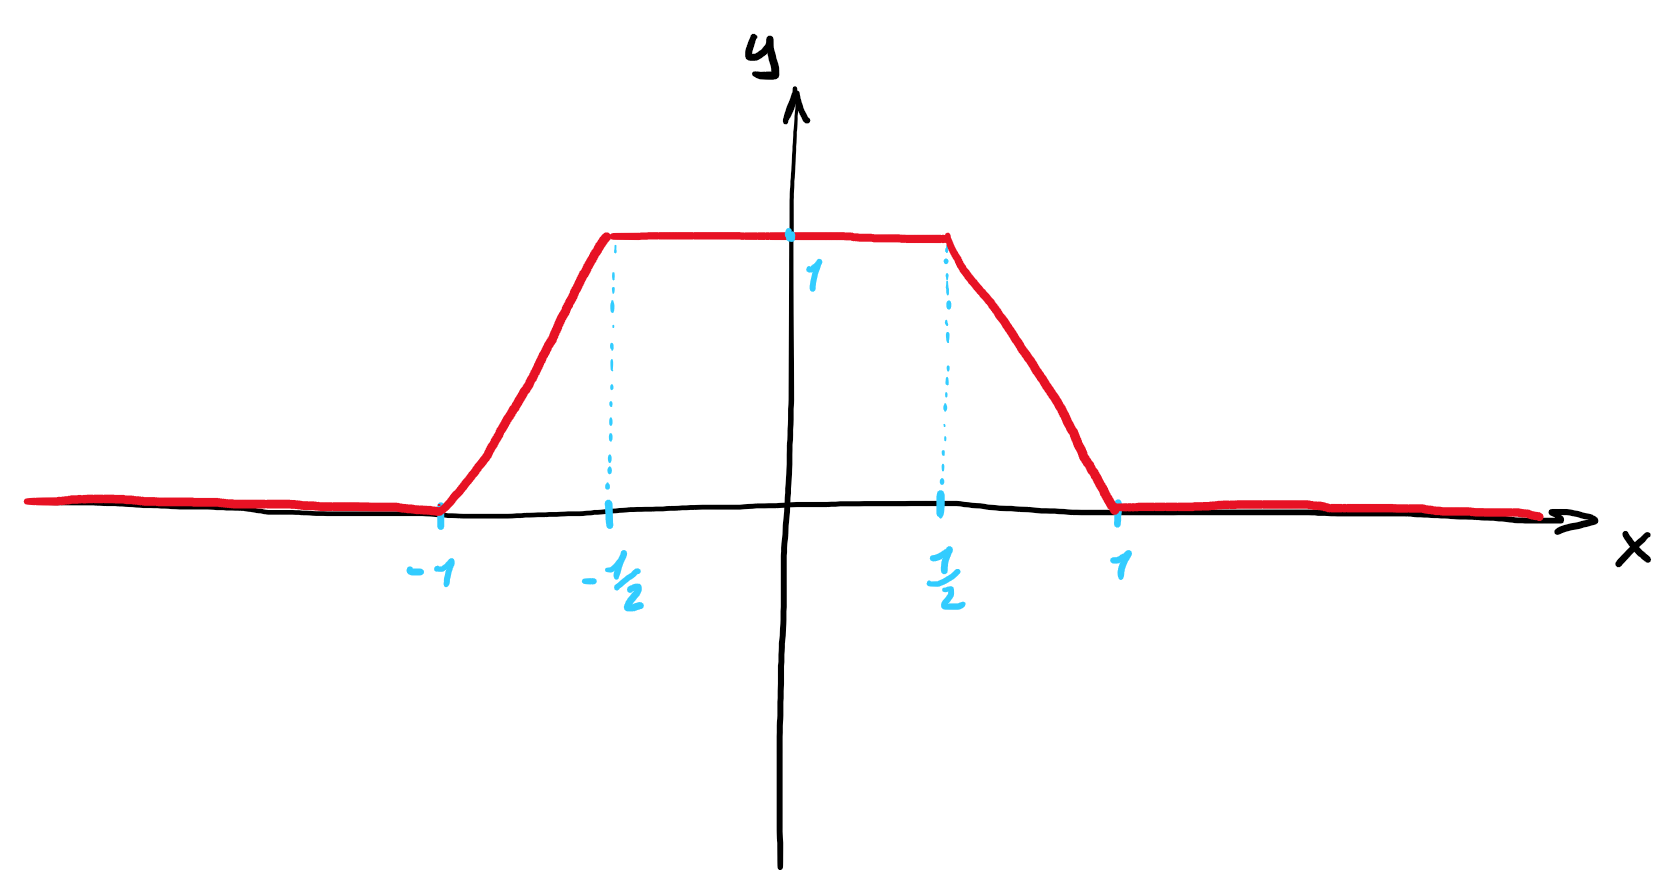
\includegraphics[width=0.7\textwidth,keepaspectratio]{img43}
\end{figure}

\begin{gather}
	Z(f) = (-\infty,-1] \cup [1,+\infty)\\
	Z(f)^{C} = (-1,-1)\\
	\operatorname{supp}(f) = \overline{Z(f)^{C}} = [-1,1]
\end{gather}

O ancora per la funzione

\begin{align}
	\begin{split}
		f : (-1,1) &\to \R\\
		x &\mapsto \tan(\dfrac{\pi x}{2})
	\end{split}
\end{align}

\begin{figure}[H]
	\centering
	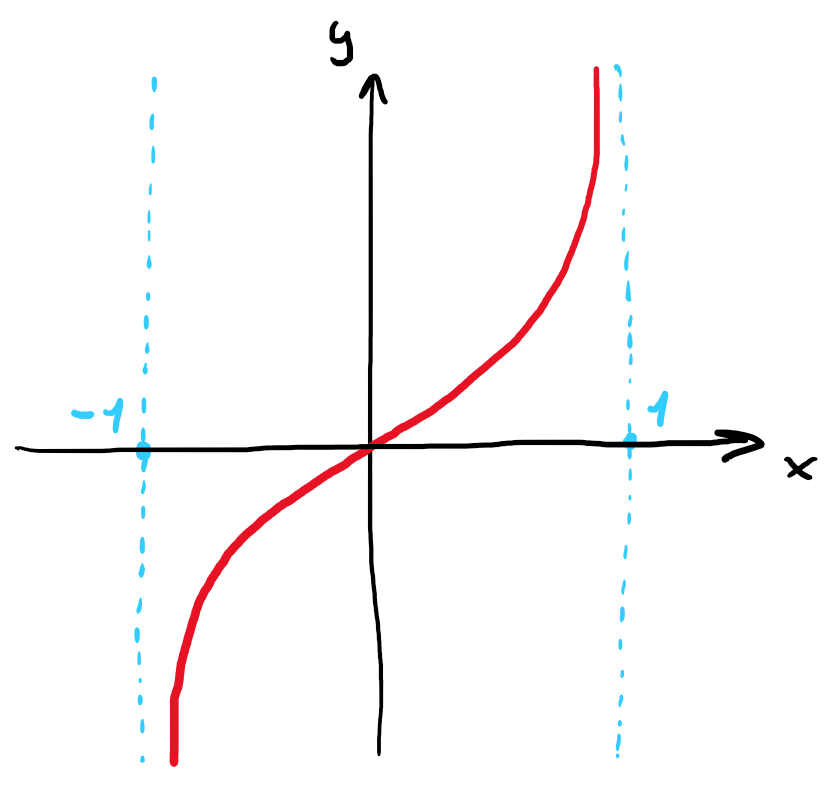
\includegraphics[width=0.3\textwidth,keepaspectratio]{img44}
\end{figure}

\begin{gather}
	Z(f) = \{0\}\\
	Z(f)^{C} = (-1,0) \cup (0,1)\\
	\operatorname{supp}(f) = \overline{Z(f)^{C}} = (-1,1)
\end{gather}

In quanto $ (-1,1) = M $ è chiuso in $ M $.\\\\
%
Siano $ M $ una varietà differenziabile, $ U \subset M $ un aperto della varietà e $ q \in U $ un suo punto, l'applicazione $ f : M \to \R $ è una \textit{funzione a campana}\footnote{%
	In inglese "bump function".%
} in $ q $ con supporto in $ U $ se

\begin{itemize}
	\item $ f $ è continua
	
	\item $ f \equiv 1 $ in un intorno di $ q $
	
	\item $ \operatorname{supp}(f) \subset U $
\end{itemize}

Il primo esempio descritto sopra è una funzione a campana in un qualsiasi punto appartenente a $ (-1,1) $ con supporto in qualunque aperto $ U \supset [-1,1] $.\\\\
%
Partendo da una funzione liscia da $ \R $ in $ \R $, costruiremo una funzione a campana liscia da $ \R^{n} $ a $ \R $.\\
Consideriamo quindi la funzione liscia

\begin{align}
	\begin{split}
		f : \R &\to \R\\
		x &\mapsto%
		\begin{cases}
			e^{\sfrac{-1}{x}} & x > 0\\
			0 & x \leqslant 0
		\end{cases}
	\end{split}
\end{align}

\begin{figure}[H]
	\centering
	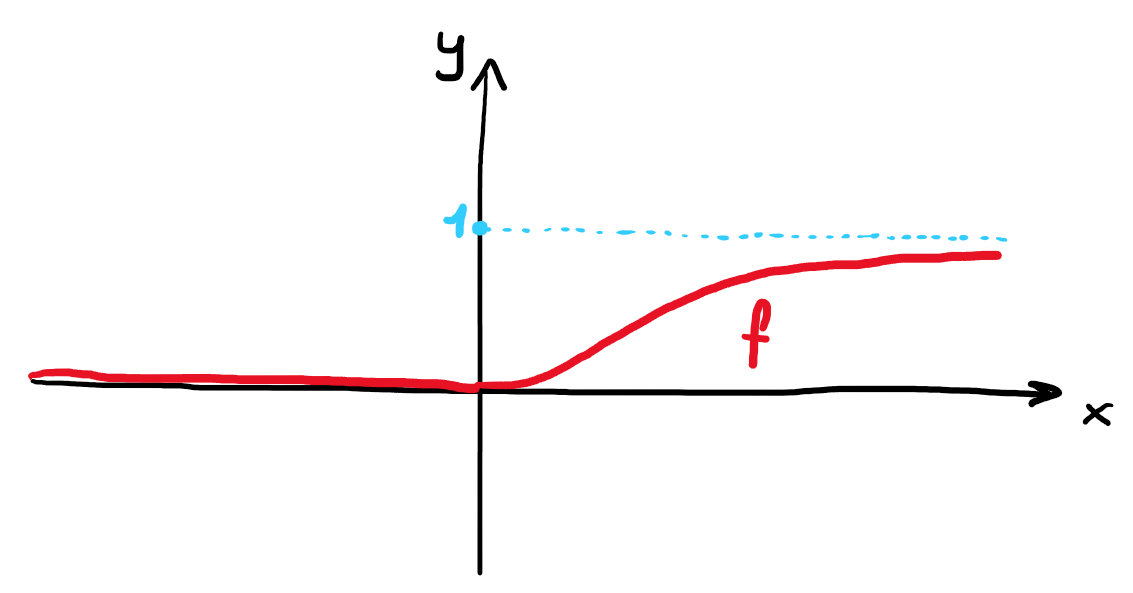
\includegraphics[width=0.5\textwidth,keepaspectratio]{img45}
\end{figure}

Il primo passo è definire una nuova funzione $ g $ a partire da $ f $ come


\begin{equation}
	g(x) = \dfrac{f(x)}{f(x) + f(1-x)}
\end{equation}

questa sarà ancora liscia se il denominatore non si annulla, in quanto

\begin{equation}
	\begin{cases}
		x \leqslant 0 \implies f(x) + f(1-x) = f(1-x) \neq 0 \quad \because \quad 1-x \geqslant 0\\
		x > 0 \implies f(x) + f(1-x) \geqslant f(x) > 0
	\end{cases}
\end{equation}

Se consideriamo il caso

\begin{equation}
	x \geqslant 1 \implies 1-x \leqslant 0 \implies f(1-x)=0 \implies g(x) = \dfrac{f(x)}{f(x)} \equiv 1
\end{equation}

perciò il grafico di $ g(x) $ avrà la forma

\begin{figure}[H]
	\centering
	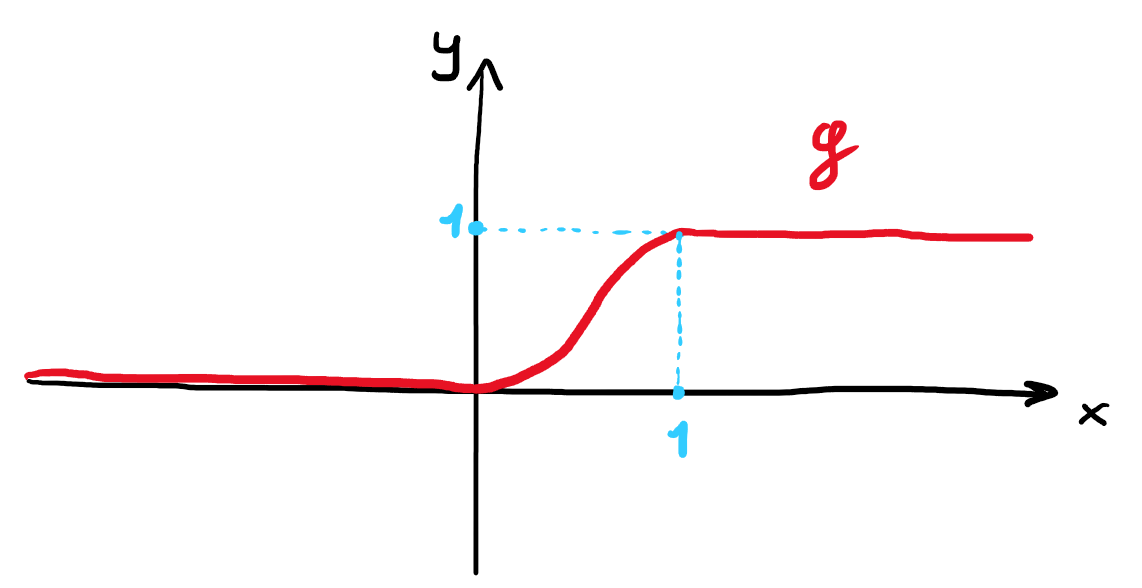
\includegraphics[width=0.5\textwidth,keepaspectratio]{img46}
\end{figure}

In modo tale da poter spostare i punti di contatto, introduciamo la seguente modifica

\begin{equation}
	h(x) = g \left( \dfrac{x - a^{2}}{b^{2} - a^{2}} \right)
\end{equation}

dove $ a,b \in \R $ e $ 0 < a < b $, perciò

\begin{equation}
	\begin{cases}
		h(x) = 1 & x \geqslant b^{2}\\
		h(x) = 0 & x \leqslant a^{2}
	\end{cases}
\end{equation}

da cui la forma "spostata"

\begin{figure}[H]
	\centering
	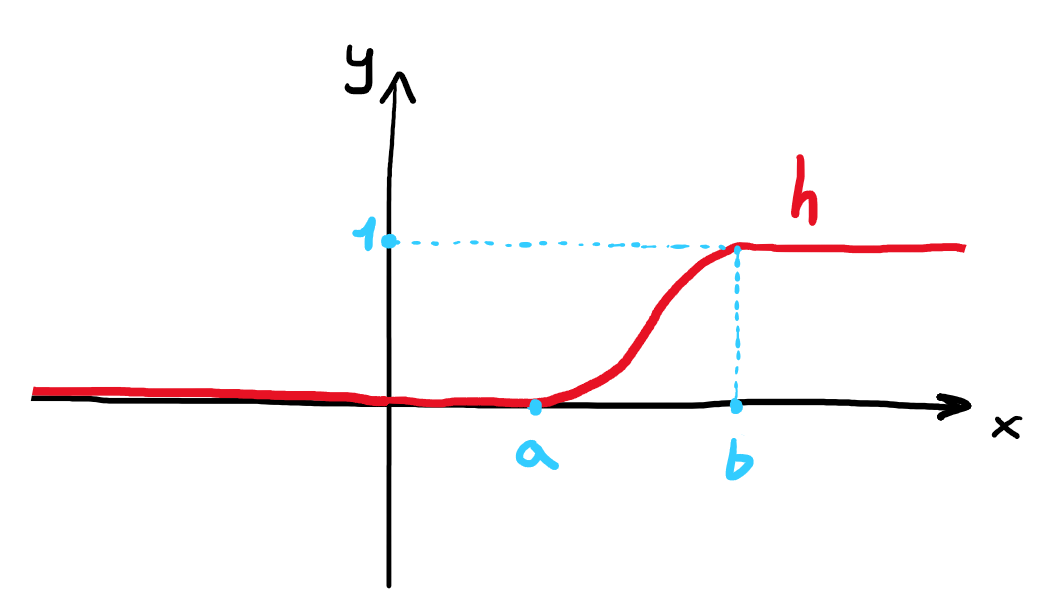
\includegraphics[width=0.5\textwidth,keepaspectratio]{img47}
\end{figure}

Il prossimo passo è rendere la funzione simmetrica

\begin{equation}
	k(x) = h(x^{2})
\end{equation}

perciò

\begin{equation}
	\begin{cases}
		k(x) = 1 & x \leqslant -b \wedge x \geqslant b\\
		k(x) = 0 & -a \leqslant x \leqslant a
	\end{cases}
\end{equation}

da cui la forma a "scodella"

\begin{figure}[H]
	\centering
	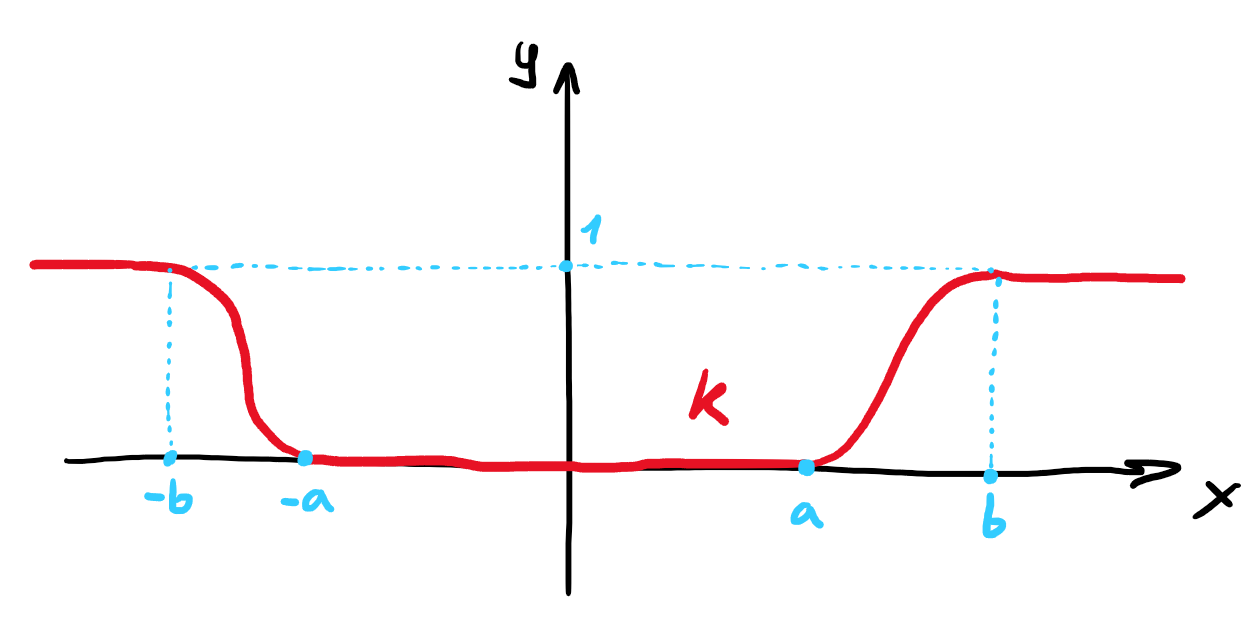
\includegraphics[width=0.5\textwidth,keepaspectratio]{img48}
\end{figure}

Considerando ora l'immagine speculare rispetto all'asse $ x $ e spostata di un'unità verso l'alto

\begin{equation}
	\sigma(x) = 1 - k(x)
\end{equation}

\begin{figure}[H]
	\centering
	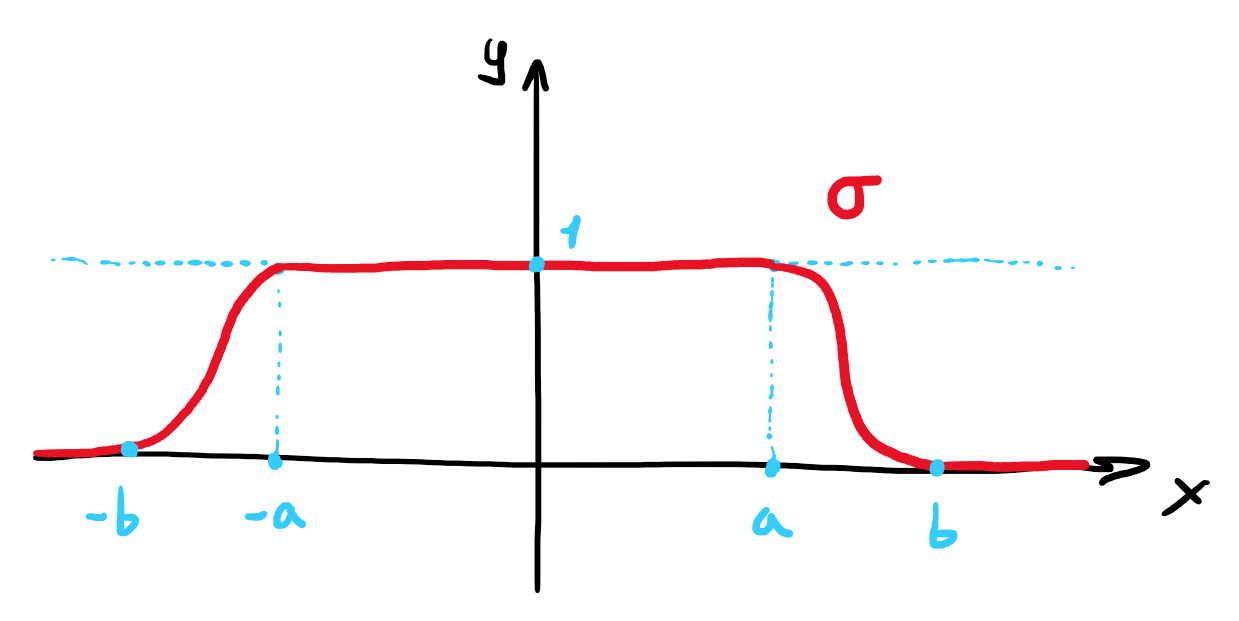
\includegraphics[width=0.5\textwidth,keepaspectratio]{img49}
\end{figure}

A questo punto, generalizziamo al dominio in $ \R^{n} $ considerando $ x = (x^{1},\dots,x^{n}) $ e poi la norma di $ x $

\begin{align}
	\begin{split}
		\rho : \R^{n} &\to \R\\
		x &\mapsto \sigma(\norm{x})
	\end{split}
\end{align}

da cui la forma in $ n+1 $ dimensioni:

\begin{figure}[H]
	\centering
	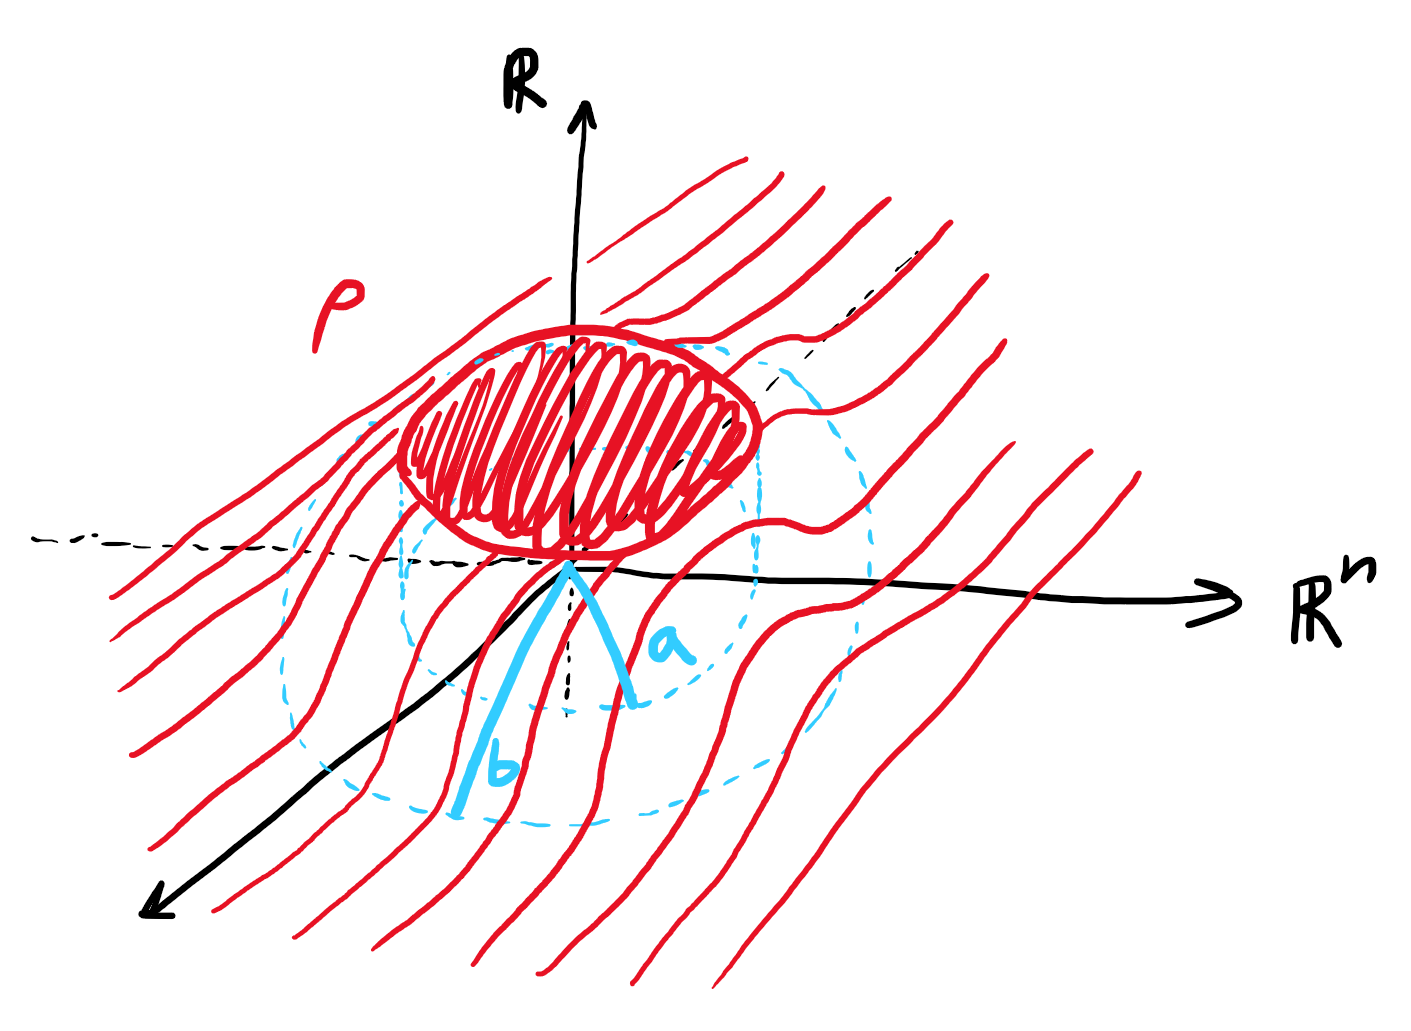
\includegraphics[width=0.5\textwidth,keepaspectratio]{img50}
\end{figure}

Considerando il disco centrato in $ q $ di raggio $ r $

\begin{equation}
	D_{r}(q) = \{ x \in \R^{n} \mid \norm{x - q} < r \}
\end{equation}

abbiamo che $ \rho $ è una funzione a campana liscia in qualsiasi punto in $ D_{a}(0) $ con supporto $ U $, dove $ U $ è un qualunque aperto tale che $ U \supset \overline{D_{b}(0)} $. I valori principali assunti dalla funzione sono per

\begin{equation}
	\begin{cases}
		\rho(x) = 1 & \forall x \in \overline{D_{a}(0)}\\\\
		\rho(x) = 0 & \forall x \in \R^{n} \setminus D_{b}(0)
	\end{cases}
\end{equation}

Si può spostare il centro della funzione in un punto $ q \in \R^{n} $ tramite la sostituzione

\begin{equation}
	\rho(x) \to \rho(x-q)
\end{equation}

Per la generalizzazione di questo procedimento a funzioni a campana su varietà, consideriamo il seguente teorema:

\begin{theorem}\label{bump-fun}
	Siano $ M $ una varietà differenziabile di dimensione $ n $, $ U \subset M $ un aperto della varietà e $ q \in U $ un suo punto, allora esiste una funzione a campana liscia $ \rho : M \to \R $ in $ q $ con supporto contenuto in $ U $.
\end{theorem}

\begin{proof}
	L'idea è di spostare il problema al costruire la funzione a campana in $ \R^{n} $.\\
	Consideriamo una carta $ (V_{r},\phi) \in M $ tale che
	
	\begin{equation}
		\begin{cases}
			q \in V_{r} \subset U\\
			\phi(q) = 0\\
			\phi(V_{r}) = D_{r}(0) \in \R^{n}
		\end{cases}
	\end{equation}

	ricordando che $ \phi $ è un diffeomorfismo e che è sempre possibile restringere l'aperto $ V_{r} $ in modo tale da avere come immagine il disco considerato.\\
	Consideriamo ora due numeri reali $ a < b < r $ e i dischi in $ \R^{n} $ centrati in 0 che hanno questi come raggio, i.e. $ D_{a}(0) \subset D_{b}(0) \subset D_{r}(0) $ dove $ \phi^{-1}(D_{a}(0)) = V_{a} $ e $ \phi^{-1}(D_{b}(0)) = V_{b} $ da cui $ V_{a} \subset V_{b} \subset V_{r} $.
	
	\begin{figure}[H]
		\centering
		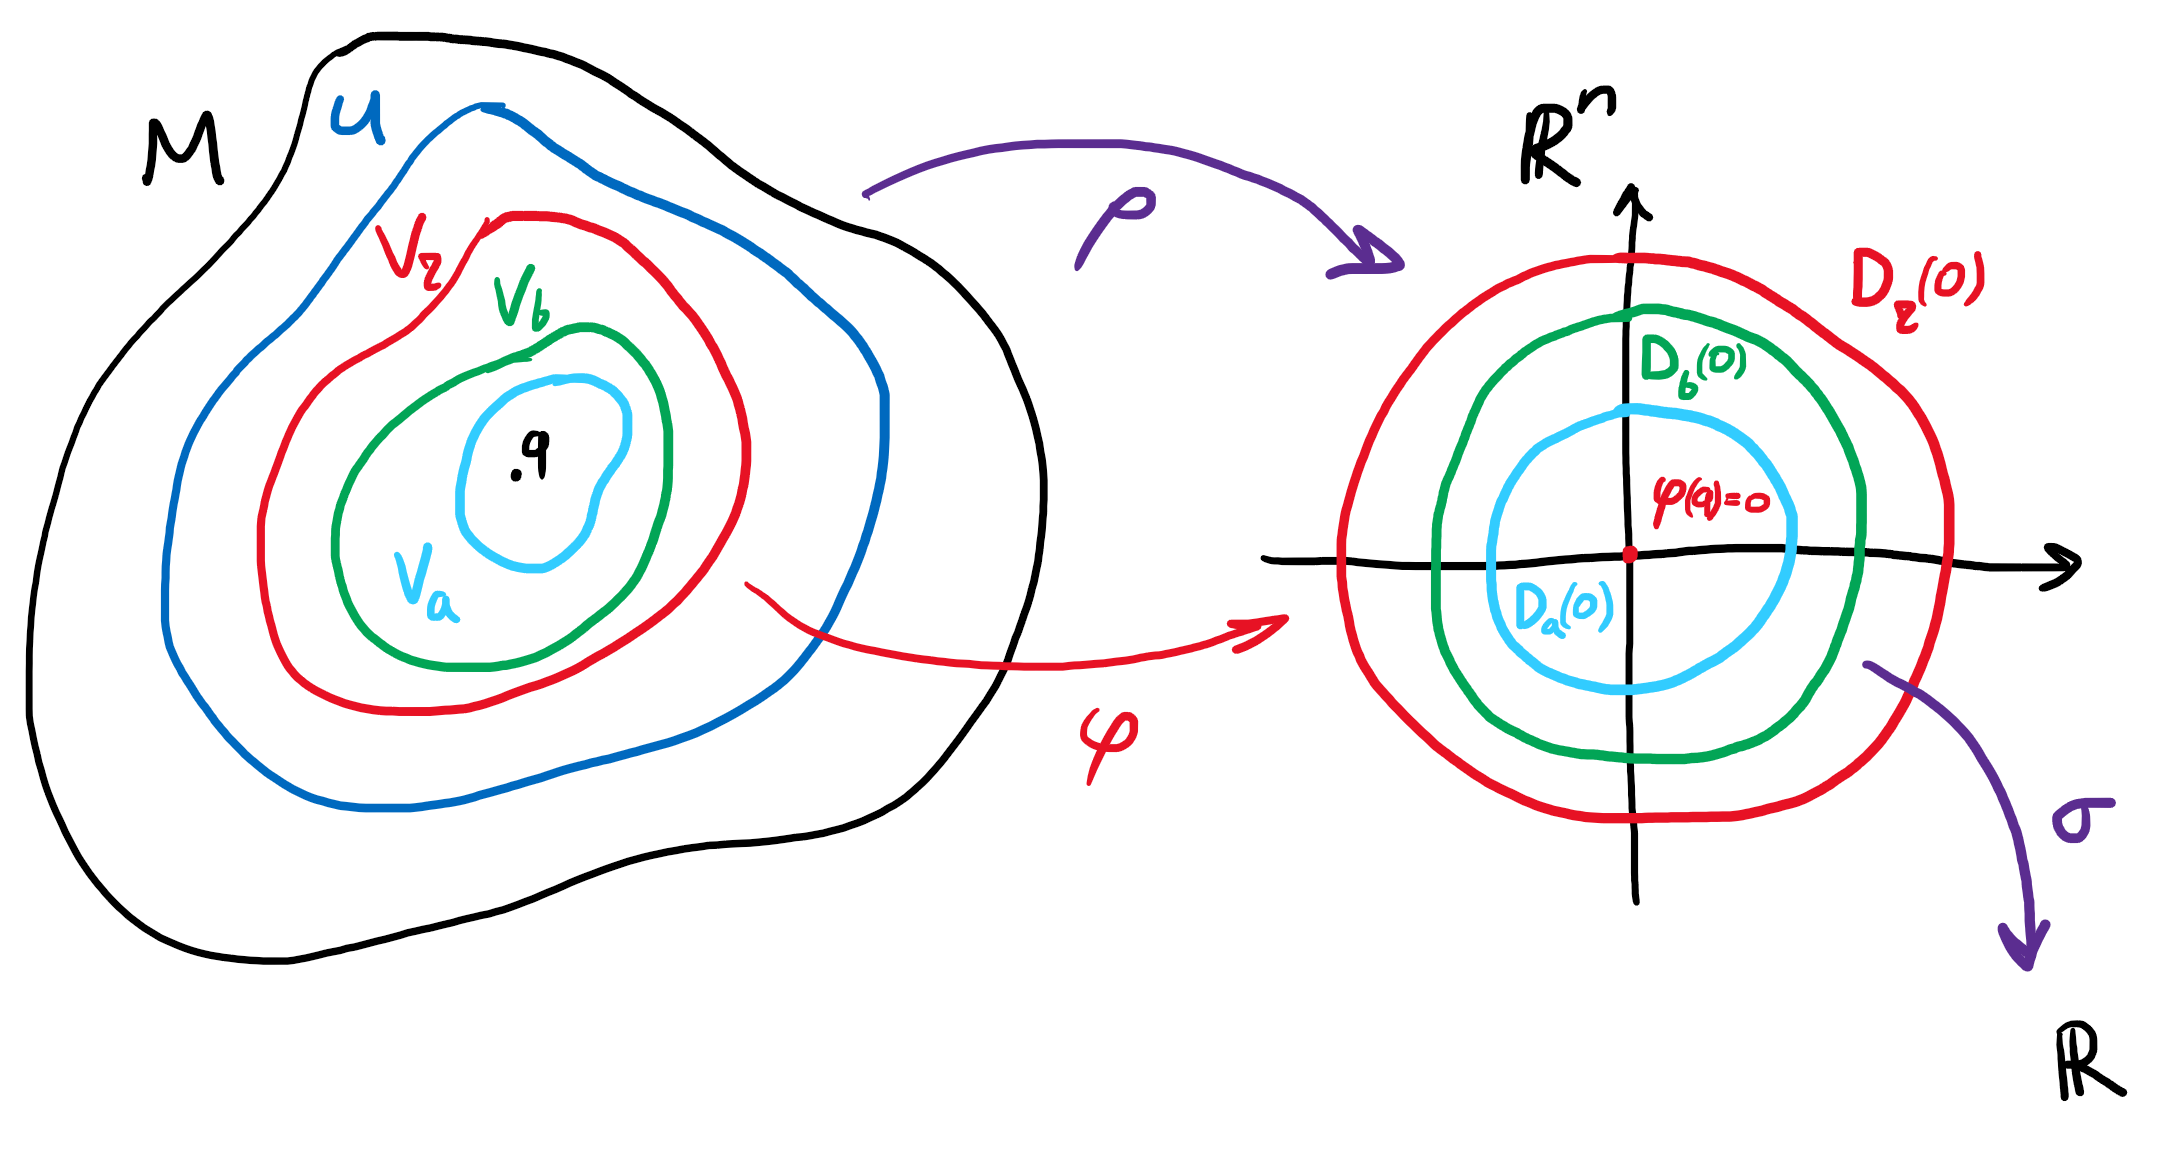
\includegraphics[width=0.8\textwidth,keepaspectratio]{img51}
	\end{figure}	
	
	Presa la funzione a campana su $ \R^{n} $
	
	\begin{equation}
		\begin{cases}
			\sigma : \R^{n} \to \R\\
			\sigma(x) = 1 & \forall x \in \overline{D_{a}(0)}\\
			\sigma(x) = 0 & \forall x \in \R^{n} \setminus D_{b}(0)\\
			\operatorname{supp}(\sigma) = \overline{D_{b}(0)}
		\end{cases}
	\end{equation}

	possiamo definire la funzione su $ M $ per $ p \in M $
	
	\begin{align}
		\begin{split}
			\rho : M &\to \R\\
			p &\mapsto %
			\begin{cases}
				(\sigma \circ \phi)(p) & p \in V_{r}\\
				0 & p \in M \setminus \overline{V_{b}}
			\end{cases}
		\end{split}
	\end{align}

	A questo punto dimostriamo che $ \rho $ sia una funzione a campana liscia in $ q $ con supporto contenuto in $ U $: è necessario che l'applicazione sia liscia, che esista un intorno in cui questa è pari a 1 e che il suo supporto sia contenuto in $ U $.
	
	\begin{itemize}
		\item Perché questa applicazione sia liscia è necessario che sia liscia per i due casi della definizione (definite in aperti) e che i valori dei due casi coincidano nell'intersezione degli aperti in cui sono definiti (la quale è ancora un aperto), i.e.
		
		\begin{equation}
			\begin{cases}
				\sigma \circ \phi \in C^{\infty}(V_{r})\\
				0 \in C^{\infty} \left( M \setminus \overline{V_{b}} \right)\\
				(\sigma \circ \phi)(p) = 0 & \forall p \in V_{r} \cap (M \setminus \overline{V_{b}})
			\end{cases}
		\end{equation}
		
		La seconda richiesta è banale e la prima è soddisfatta in quanto composizione di funzioni lisce; per la terza, possiamo scrivere
		
		\begin{equation}
			V_{r} \cap \left( M \setminus \overline{V_{b}} \right) = V_{r} \setminus \overline{V_{b}}
		\end{equation}
		
		essendo $ \sigma(x) = 0 $ per $ \forall x \in \R^{n} \setminus D_{b}(0) $, possiamo dunque scrivere
		
		\begin{equation}
			(\sigma \circ \phi)(p) = 0, \qquad \forall p \in V_{r} \setminus \overline{V_{b}}
		\end{equation}
		
		%
		
		\item Abbiamo che $ V_{a} \ni q $ e che
		
		\begin{equation}
			\rho(p) \equiv 1, \qquad \forall p \in V_{a}
		\end{equation}
	
		perciò esiste un intorno di $ q $ (in questo caso $ V_{a} $) in cui la funzione è pari a 1
		
		%
		
		\item Abbiamo che
		
		\begin{equation}
			\operatorname{supp}(\sigma) = \overline{D_{b}(0)}
		\end{equation}
	
		e che $ \phi $ è un diffeomorfismo, dunque il supporto di $ \rho $ sarà
		
		\begin{equation}
			\operatorname{supp}(\rho) = \phi \left( \overline{D_{b}(0)} \right) = \overline{V_{b}} \subset V_{r} \subset U
		\end{equation}
	\end{itemize}
	
	Questo prova dunque che esiste una funzione a campana liscia per ogni punto di una varietà con supporto contenuto in un intorno del punto.
\end{proof}

\begin{corollary}[Estensione di funzioni lisce]\label{cor-est-smooth}
	Siano $ M $ una varietà differenziabile, un punto $ p \in M $, un aperto $ U \subset M $ che sia intorno di $ p $ e una funzione $ f : M \to \R $ liscia solo su $ U $, i.e. $ f \in C^{\infty}(U) $, allora esistono un aperto $ V \subseteq U $ intorno di $ q $ e una funzione $ \tilde{f} : M \to \R $ liscia in tutta la varietà $ \tilde{f} \in C^{\infty}(M) $ tale che $ \tilde{f} \equiv f $ in $ V $; in pratica, $ \tilde{f} $ è un'estensione di $ f_{|V} $.
\end{corollary}

In generale non si può estendere una funzione oltre al dominio in cui essa è liscia però, tramite questo corollario, è possibile considerare la restrizione a un aperto di questa funzione ed estenderla in modo liscio. Un esempio è la funzione $ f(x) = \tan(\sfrac{x}{2}) $ la quale ha due asintoti verticali in $ \pm \pi $: prendendo un aperto $ V \subset [-\pi,\pi] $ e la restrizione di $ f $ ad esso, è possibile "incollare" in modo liscio alla funzione due estensioni di questa oltre il suo dominio.

\begin{proof}
	Sia $ \rho : M \to \R $ una funzione liscia a campana in $ q $ con supporto contenuto in $ U $ (esiste per il teorema precedente) che sia uguale a 1 nell'aperto $ V $.\\
	Definiamo
	
	\begin{align}
		\begin{split}
			\tilde{f} : M &\to \R\\
			p &\mapsto %
			\begin{cases}
				(\rho \circ f)(p) & p \in U\\
				0 & p \in M \setminus \operatorname{supp}(\rho)
			\end{cases}
		\end{split}
	\end{align}

	Perché sia liscia è necessario che lo sia nei due casi della definizione e che questi coincidano nella loro intersezione: per quest'ultima richiesta, possiamo scrivere l'intersezione come
	
	\begin{equation}
		U \cap (M \setminus \operatorname{supp}(\rho)) = U \setminus \operatorname{supp}(\rho)
	\end{equation}

	la quale è aperta perché il supporto è un chiuso, dunque resta verificare che i casi coincidano, ricordando che
	
	\begin{equation}
		\rho(p) = 0, \qquad \forall p \in M \setminus \operatorname{supp}(\rho)
	\end{equation}

	perciò
	
	\begin{equation}
		\tilde{f}(p) = (\rho \circ f)(p) = 0, \qquad \forall p \in U \setminus \operatorname{supp}(\rho)
	\end{equation}

	dunque la funzione è liscia dappertutto.\\
	L'altra richiesta è che $ \tilde{f} \equiv f $ in $ V $: anche questo è verificato perché
	
	\begin{equation}
		\rho(p) \equiv 1, \quad \forall p \in V \implies \tilde{f}(p) = (\rho \circ f)(p) \equiv f(p), \quad \forall p \in V
	\end{equation}
\end{proof}

\subsection{Campi di vettori su varietà}

Sia $ M $ una varietà differenziabile di dimensione $ m $. Ricordando la definizione del fibrato tangente

\begin{equation}
	T(U) = \bigsqcup_{p \in M} T_{p}(M)
\end{equation}

e della proiezione preso un vettore $ (p,v) \equiv X_{p} \in T_{p}(M) $

\begin{align}
	\begin{split}
		\pi : T(M) &\to M\\
		X_{p} &\mapsto p
	\end{split}
\end{align}

un \textit{campo di vettori} è un'applicazione

\begin{align}
	\begin{split}
		X : M &\to T(M)\\
		p &\mapsto X_{p}
	\end{split}
\end{align}

e dunque $ \pi \circ X = \id_{M} $.\\\\
%
Localmente, un campo di vettori $ X $ su una varietà $ M $ è \textit{liscio} se per $ \forall p \in M $ esiste una carta $ (U,\phi) \in M $ con $ \phi = (x^{1},\dots,x^{n}) $ intorno a $ p $ tale che, scrivendo il vettore $ X_{p} \in T_{p}(M) $ tangente alla varietà $ M $ nel punto $ p \in U $ come

\begin{equation}
	X_{p} = \sum_{j=1}^{n} a^{j}(p) \left. \dfrac{\partial}{\partial x^{j}} \right|_{p} 
\end{equation}

le funzioni $ a^{j} : U \to \R $ sono lisce in $ U $, da cui l'espressione locale dei vettori del campo

\begin{equation}
	X_{|U} = \sum_{j=1}^{n} a^{j} \dfrac{\partial}{\partial x^{j}}
\end{equation}

La definizione non dipende dalla carta scelta: presa un'altra carta $ (V,\psi) \in M $ con $ \psi = (y^{1},\dots,y^{n}) $ intorno a $ p $, $ X_{p} $ si scriverà come

\begin{equation}
	X_{|V} = \sum_{j=1}^{n} b^{j} \dfrac{\partial}{\partial y^{j}} 
\end{equation}

nell'intersezione degli aperti delle carte, i.e. $ U \cap V $, possiamo dunque scrivere che

\begin{align}
	\begin{split}
		a^{j} &= \sum_{j=1}^{n} b^{k} \, \dfrac{\partial x^{j}}{\partial y^{k}}\\
		b^{j} &= \sum_{j=1}^{n} a^{k} \, \dfrac{\partial y^{j}}{\partial x^{k}}
	\end{split}
\end{align}

per $ \forall j=1,\dots,n $, da cui

\begin{equation}
	a^{j} \in C^{\infty}(U) \iff b^{j} \in C^{\infty}(V)
\end{equation}

perché lo sono le entrate delle matrici jacobiane sono lisce.\\\\
%
\`{E} possibile definire un campo liscio anche mediante la seguente proposizione:

\begin{definition}
	Sia $ X $ un campo di vettori su $ M $, allora $ X : M \to T(M) $ è un'applicazione liscia se e solo se il campo di vettori è liscio, i.e. se scrivendo
	
	\begin{equation}
		X_{|U} = \sum_{j=1}^{n} a^{j} \dfrac{\partial}{\partial x^{j}}
	\end{equation}

	si ha che $ a^{j} \in C^{\infty}(U) $.
\end{definition}

\begin{proof}[Dimostrazione ($ \implies $)]
	Siano $ X : M \to T(M) $ un'applicazione liscia e $ (U,\phi) \in M $ con $ \phi = (x^{1},\dots,x^{n}) $ intorno a $ p $ una carta di $ M $. Possiamo scrivere il campo di vettori come
	
	\begin{equation}
		X_{|U} = \sum_{j=1}^{n} a^{j} \dfrac{\partial}{\partial x^{j}}
	\end{equation}

	con $ a^{j} : U \to \R $.\\
	Sia una carta $ (T(U),\tilde{\phi}) \in T(M) $ con il diffeomorfismo
	
	\begin{align}
		\begin{split}
			\tilde{\phi} : T(U) &\to \phi(U) \times \R^{n}\\
			X_{p} &\mapsto (\phi(p),c(X_{p}))\\
			&\mapsto (x^{1}(p),\dots,x^{n}(p),c^{1}(X_{p}),\dots,c^{n}(X_{p}))
		\end{split}
	\end{align}

	dove $ c(X_{p}) = (c^{1}(X_{p}),\dots,c^{n}(X_{p})) $ con $ c^{j} \in C^{\infty}(T(U)) $ e
	
	\begin{equation}
		X_{p} = \sum_{j=1}^{n} c^{j}(X_{p}) \left. \dfrac{\partial}{\partial x^{j}} \right|_{p}
	\end{equation}

	da cui possiamo considerare la restrizione
	
	\begin{equation}
		X_{|U} = \sum_{j=1}^{n} c^{j} \dfrac{\partial}{\partial x^{j}}
	\end{equation}

	e dunque $ c^{j} \circ \pi = a^{j} $, il che implica che $ a^{j} \in C^{\infty}(U) $.
\end{proof}

\begin{proof}[Dimostrazione ($ \impliedby $)]
	Supponiamo di poter scrivere
	
	\begin{equation}
		X_{|U} = \sum_{j=1}^{n} a^{j} \dfrac{\partial}{\partial x^{j}}
	\end{equation}
	
	con $ a^{j} \in C^{\infty}(U) $.\\
	Consideriamo la composizione
	
	\begin{align}
		\begin{split}
			\tilde{\phi} \circ X_{|U} : U &\to T(U) \to \phi(U) \times \R^{n}\\
			p &\mapsto (\phi(p),c(X_{p}))
		\end{split}
	\end{align}

	da cui
	
	\begin{align}
		\begin{split}
			(\tilde{\phi} \circ X_{|U})(p) &= \tilde{\phi}(X_{p})\\
			&= (\phi(p),c(X_{p}))\\
			&= (\phi(p),a(p))
		\end{split}
	\end{align}

	Da questo risultato, siccome $ \phi $  un diffeomorfismo e le $ a^{j} $ sono lisce, abbiamo che la composizione $ \tilde{\phi} \circ X_{|U} $ è liscia: essendo anche $ \tilde{\phi} $ un diffeomorfismo, $ X_{|U} $ è liscio localmente e dunque lo è anche globalmente, i.e. $ X \in C^{\infty}(M) $.
\end{proof}

L'insieme dei campi di vettori lisci verrà indicato come

\begin{equation}
	\chi(M) = \{ \text{campi di vettori } X \text{ su } M \}
\end{equation}

\subsubsection{$ \chi(M) $ come $ C^{\infty}(M) $-modulo}

\begin{definition}
	L'insieme $ \chi(M) $ è un $ C^{\infty}(M) $-modulo.
\end{definition}

\begin{proof}
	Vedi Teorema \ref{chi-mod}.
\end{proof}

Perché $ \chi(M) $ sia un $ C^{\infty}(M) $-modulo è necessario che sia uno spazio vettoriale sul campo dei reali, i.e.

\begin{equation}
	\begin{cases}
		\lambda X + \mu Y \in \chi(M) & \forall X,Y \in \chi(M), \, \forall \lambda,\mu \in \R\\
		(\lambda X + \mu Y)_{p} = \lambda X_{p} + \mu Y_{p}
	\end{cases}
\end{equation}

Inoltre, si deve poter moltiplicare il campo per una funzione liscia: usiamo per questo la seguente applicazione

\begin{align}
	\begin{split}
		K : C^{\infty}(M) \times \chi(M) &\to \chi(M)\\
		(f,X) &\mapsto f X
	\end{split}
\end{align}

con la condizione che

\begin{equation}
	(f X)(p) = f(p) \, X_{p}
\end{equation}

da cui

\begin{equation}
	\begin{cases}
		f X \in \chi(M)\\
		X_{|U} = \sum_{j=1}^{n} a^{j} \dfrac{\partial}{\partial x^{j}}
	\end{cases}%
	\implies%
	f X_{|U} = \sum_{j=1}^{n} f a^{j} \dfrac{\partial}{\partial x^{j}}
\end{equation}

dove le funzioni $ f a^{j} $ sono lisce. Essendo quindi $ \chi(M) $ un $ C^{\infty}(M) $-modulo, sono possibili tutte le combinazioni lineari con campi e funzioni, i.e.

\begin{equation}
	(f+g)(X) = f X + g X
\end{equation}

\subsubsection{Derivata di una funzione rispetto a un campo di vettori}

Siano $ X \in \chi(M) $ e $ f \in C^{\infty}(M) $, allora la derivata della funzione $ f $ rispetto al campo di vettori $ X $ è definita come la funzione

\begin{align}
	\begin{split}
		X f : M &\to \R\\
		p &\mapsto (X f)(p) = X_{p} f
	\end{split}
\end{align}

La derivata può anche essere definita si germi delle funzioni in quanto tutte le funzioni di uno stesso germe coincidono in un intorno del punto, i.e.

\begin{equation}
	X_{p} f = X_{p} [f], \qquad f \in [f] \in C_{p}^{\infty}(M)
\end{equation}

\begin{definition}
	Fissato un campo di vettori $ X \in \chi(M) $, l'immagine della funzione
	
	\begin{align}
		\begin{split}
			\Phi(X) : C^{\infty}(M) &\to C^{\infty}(M)\\
			f &\mapsto X f
		\end{split}
	\end{align}

	è una funzione liscia, i.e. $ X f \in C^{\infty}(M) $.
\end{definition}

\begin{proof}
	\`{E} sufficiente dimostrare che la funzione
	
	\begin{align}
		\begin{split}
			X f : M &\to \R\\
			p &\mapsto X_{p} f
		\end{split}
	\end{align}

	sia liscia.\\
	Siano $ p \in M $ un punto della varietà e $ (U,\phi) \in M $ con $ \phi = (x^{1},\dots,x^{n}) $ intorno a $ p $ una carta di $ M $, allora
	
	\begin{equation}
		X_{|U} = \sum_{j=1}^{n} a^{j} \dfrac{\partial}{\partial x^{j}}
	\end{equation}

	perciò
	
	\begin{equation}
		(X f)_{|U} = \sum_{j=1}^{n} a^{j} \dfrac{\partial f}{\partial x^{j}}
	\end{equation}

	in quanto
	
	\begin{equation}
		X_{p} f = \sum_{j=1}^{n} a^{j}(p) \dfrac{\partial f}{\partial x^{j}} (p)
	\end{equation}

	i quali sono lisci perché le $ a^{j} $ e le derivate parziali $ \sfrac{\partial f}{\partial x^{j}} $ sono lisce.\\
	Avendo fatto vedere che $ X f $ è localmente liscia, allora lo è anche globalmente.
\end{proof}

\begin{definition}
	Un campo di vettori $ X $ è liscio se e solo se la derivata $ X f $ è liscia per ogni funzione $ f $, i.e.
	
	\begin{equation}
		X \in \chi(M) \iff X f \in C^{\infty}(M), \, \forall f \in C^{\infty}(M)
	\end{equation}
\end{definition}

\begin{proof}[Dimostrazione ($ \implies $)]
	Vedi dimostrazione della proposizione precedente.
\end{proof}

\begin{proof}[Dimostrazione ($ \impliedby $)]
	Supponiamo che
	
	\begin{equation}
		X f \in C^{\infty}(M), \qquad \forall f \in C^{\infty}(M)
	\end{equation}

	Sia $ (U,\phi) \in M $ con $ \phi = (x^{1},\dots,x^{n}) $ intorno a $ p $ una carta di $ M $, allora
	
	\begin{equation}
		X_{|U} = \sum_{j=1}^{n} a^{j} \dfrac{\partial}{\partial x^{j}}
	\end{equation}

	con $ a^{j} : U \to \R $ per $ \forall j=1,\dots,n $. Perché $ X \in \chi(M) $ dobbiamo dimostrare che $ a^{j} \in C^{\infty}(U) $.\\
	Per il corollario di estensione di funzioni\footnote{%
		Vedi Corollario \ref{cor-est-smooth}.%
	}, esistono un aperto $ V \subset U \ni p $ e delle funzioni $ \tilde{x}^{k} \in C^{\infty}(M) $ tali che $ \tilde{x}^{k}_{|V} \equiv x^{k} $ per $ \forall k=1,\dots,n $ (dalla carta, $ x^{k} \in C^{\infty}(U) $ per $ \forall k=1,\dots,n $). Applichiamo ora la derivata a queste estensioni
	
	\begin{align}
		\begin{split}
			(X \tilde{x}^{k})_{|V} &= \left( \sum_{j=1}^{n} a^{j} \dfrac{\partial}{\partial x^{j}} \right) (\tilde{x}^{k})_{|V}\\
			&= \left( \sum_{j=1}^{n} a^{j} \dfrac{\partial}{\partial x^{j}} \right) (x^{k})\\
			&= \sum_{j=1}^{n} a^{j} \dfrac{\partial x^{k}}{\partial x^{j}}\\
			&= a^{j} \delta^{kj}\\
			&= a^{k}
		\end{split}
	\end{align}

	Essendo $ (X \tilde{x}^{k})_{|V} $ liscio per ipotesi, abbiamo che le $ a^{k} \in C^{\infty}(V) $ da cui si ottiene che queste sono lisce in tutto $ M $, in quanto il punto $ p $ considerato è arbitrario, e dunque $ X \in \chi(M) $.
\end{proof}

\subsubsection{Proprietà}

Riassumendo, sono presenti tre metodi equivalenti per determinare se un campo $ X $ su $ M $ sia liscio, i.e. $ X \in \chi(M) $:

\begin{enumerate}
	\item Considerata $ (U,\phi) \in M $ con $ \phi = (x^{1},\dots,x^{n}) $ intorno a $ p \in M $ una carta di $ M $, è possibile scrivere il campo localmente come
	
	\begin{equation}
		X_{|U} = \sum_{j=1}^{n} a^{j} \dfrac{\partial}{\partial x^{j}}
	\end{equation}

	dove le $ a^{j} \in C^{\infty}(U) $ per $ \forall j=1,\dots,n $;
	
	\item Si può vedere il campo come un'applicazione liscia
	
	\begin{align}
		\begin{split}
			X : M &\to T(M)\\
			p &\mapsto X_{p} \in T_{p}(M)
		\end{split}
	\end{align}
	
	tale che $ \pi \circ X = \id_{M} $ dove $ \pi(X_{p})=p $;
	
	\item La derivata direzionale di una funzione è liscia per ogni funzione liscia, i.e. l'immagine dell'applicazione
	
	\begin{align}
		\begin{split}
			\Phi(X) : C^{\infty}(M) &\to C^{\infty}(M)\\
			f &\mapsto X f
		\end{split}
	\end{align}

	è liscia.
\end{enumerate}

Ricordiamo che la derivata $ X f $ si scrive come

\begin{equation}
	(X f)(p) = X_{p} f \equiv X_{p} [f]
\end{equation}

in quanto $ f \in [f] \in C_{p}^{\infty}(M) $ e la derivata non dipende dal rappresentante scelto dal germe.

\paragraph{Uguaglianza tra campi di vettori}

\begin{theorem}[Uguaglianza tra campi di vettori]
	Siano $ X,Y \in \chi(M) $, allora
	
	\begin{equation}
		X = Y \iff X f = Y f, \qquad \forall f \in C^{\infty}(M)
	\end{equation}
\end{theorem}

\begin{proof}[Dimostrazione ($ \implies $)]
	La prima implicazione è banale in quanto, se due campi di vettori $ X,Y \in \chi(M) $ sono uguali allora anche lo è anche la loro azione su una funzione liscia $ f $, i.e.
	
	\begin{equation}
		X = Y \implies X f = Y f, \qquad \forall f \in C^{\infty}(M)
	\end{equation}
\end{proof}

\begin{proof}[Dimostrazione ($ \impliedby $)]
	Supponiamo che $ X f = Y f $ per $ \forall f \in C^{\infty}(M) $.\\
	Andando a ritroso, abbiamo la seguente serie di implicazioni:
	
	\begin{equation}
		X = Y \iff X_{p} = Y_{p}, \qquad \forall p \in M
	\end{equation}

	considerando l'azione sui germi
	
	\begin{equation}
		\begin{aligned}
			X_{p} = Y_{p}\\
			\forall p \in M
		\end{aligned}%
		 \iff %
		 \begin{aligned}
			 X_{p} [h] &= Y_{p} [h]\\
			 \forall p \in M,& \quad \forall [h] \in C_{p}^{\infty}(M)
		 \end{aligned}
	\end{equation}

	prendendo un rappresentante
	
	\begin{equation}
		\begin{aligned}
			X_{p} [h] &= Y_{p} [h]\\
			\forall p \in M,& \quad \forall [h] \in C_{p}^{\infty}(M)
		\end{aligned}%
		\iff %
		\begin{aligned}
			X_{p} h &= Y_{p} h\\
			\forall p \in M,& \quad \forall h \in C^{\infty}(U)
		\end{aligned}
	\end{equation}
	
	dove $ h \in [h] $ e $ U \ni p $.\\
	L'ipotesi però comprende funzioni $ \forall f \in C^{\infty}(M) $ dunque, tramite il corollario di estensione di funzioni lisce, consideriamo un aperto $ V \subset U $ che contenga $ p $ e $ \tilde{h} \in C^{\infty}(M) $ tale che $ \tilde{h} \equiv h $ nell'aperto $ V $.\\
	Applichiamo l'ipotesi a questa funzione
	
	\begin{equation}
		X \tilde{h} = Y \tilde{h} \iff (X \tilde{h})(p) = (Y \tilde{h})(p), \qquad p \in M
	\end{equation}

	e dunque
	
	\begin{equation}
		X_{p} \tilde{h} = Y_{p} \tilde{h} \iff X_{p} h = Y_{p} h
	\end{equation}

	perché $ \tilde{h} \equiv h $ in $ V $ (equivalentemente $ \tilde{h} \sim h $) e questo, tramite i passaggi iniziali, porta a $ X = Y $.
\end{proof}

\paragraph{$ \R $-linearità}

Considerato $ X \in \chi(M) $, possiamo dimostrare che l'applicazione

\begin{align}
	\begin{split}
		\Phi(X) : C^{\infty}(M) &\to C^{\infty}(M)\\
		f &\mapsto X f
	\end{split}
\end{align}

sia $ \R $-lineare, i.e.

\begin{equation}
	\Phi(X)(\lambda f + \mu g) = \lambda \Phi(X)(f) + \mu \Phi(X)(g), \qquad \forall \lambda,\mu \in \R, \, \forall f,g \in C^{\infty}(M)
\end{equation}

\begin{proof}
	Preso un punto arbitrario $ p \in M $
	
	\begin{align}
		\begin{split}
			\Phi(X)(\lambda f + \mu g)(p) &= X(\lambda f + \mu g)(p)\\
			&= X_{p}(\lambda f + \mu g)\\
			&= \lambda X_{p} f + \mu X_{p} g\\
			&= \lambda (X f)(p) + \mu (X g)(p)\\
			&= (\lambda X f + \mu X g)(p)\\
			&= (\lambda \Phi(X)(f) + \mu \Phi(X)(g))(p)
		\end{split}
	\end{align}

	in quanto $ X_{p} \in T_{p}(M) = \der_{p}(C_{p}^{\infty}(M)) $ e quindi $ \R $-lineare.
\end{proof}

\paragraph{Regola di Leibniz}

I campi di vettori lisci rispettano la regola di Leibniz:

\begin{equation}
	X(f g) = (X f) g + f (X g), \qquad \forall f,g \in C^{\infty}(M)
\end{equation}

\begin{proof}
	Preso un punto arbitrario $ p \in M $
	
	\begin{align}
		\begin{split}
			X(f g)(p) &= X_{p}(f g)\\
			&= (X_{p} f) \, g(p) + f(p) \, (X_{p} g)\\
			&= (X f)(p) \, g(p) + f(p) \, (X g)(p)\\
			&= ((X f) g + f (X g))(p)
		\end{split}
	\end{align}
	
	in quanto $ X_{p} \in T_{p}(M) = \der_{p}(C_{p}^{\infty}(M)) $ (i.e. si possono omettere le classi e considerare direttamente i rappresentanti di esse) e quindi rispetta la regola di Leibniz.
\end{proof}

\subsubsection{Derivazioni dell'algebra}

A questo punto, possiamo scrivere l'insieme delle derivazioni dell'algebra $ C^{\infty}(M) $

\begin{equation}
	Der(C^{\infty}(M)) = \{ D : C^{\infty}(M) \to C^{\infty}(M) \mid D \text{ è } \R-\text{lineare e soddisfa Leibniz} \}
\end{equation}

il quale è uno spazio vettoriale su $ \R $ con operazioni

\begin{equation}
	\begin{cases}
		(D_{1} + D_{2})(f) = D_{1}(f) + D_{2}(f) & \forall D_{1},D_{2} \in Der(C^{\infty}(M))\\
		(\lambda D)(f) = \lambda (D f) & \forall \lambda \in \R, \, \forall D \in Der(C^{\infty}(M))
	\end{cases}
\end{equation}

La dimostrazione è la stessa fatta per aperti di $ \R^{n} $.\\
Le derivazioni $ Der(C^{\infty}(M)) $ sono anche un $ C^{\infty}(M) $-modulo: il primo requisito è che siano uno spazio vettoriale e il secondo è che si possa moltiplicare una derivazione per una funzione liscia, come dalla seguente applicazione

\begin{align}
	\begin{split}
		K : C^{\infty}(M) \times Der(C^{\infty}(M)) &\to Der(C^{\infty}(M))\\
		(f,D) &\mapsto f D
	\end{split}
\end{align}

definendo l'azione dell'immagine di questa funzione come

\begin{equation}
	(f D)(g) \doteq f (D(g)), \qquad \forall g \in C^{\infty}(M)
\end{equation}

La dimostrazione è la stessa fatta per aperti di $ \R^{n} $.

\subsubsection{$ \chi(M) \simeq Der(C^{\infty}(M)) $}

\begin{theorem}
	Sia l'applicazione
	
	\begin{align}
		\begin{split}
			\Phi : \chi(M) &\to Der(C^{\infty}(M))\\
			X &\mapsto \Phi(X)
		\end{split}
	\end{align}

	dove l'azione dell'immagine è quella dell'applicazione definita in precedenza per i campi di vettori, i.e.
	
	\begin{equation}
		\Phi(X)(f) = X f
	\end{equation}

	L'applicazione $ \Phi $ è un isomorfismo di $ C^{\infty}(M) $-moduli.
\end{theorem}

Per la dimostrazione, è necessario il seguente lemma:

\begin{lemma}
	Siano $ D \in Der(C^{\infty}(M)) $ e $ \tilde{f} \in C^{\infty}(M) $ tale che $ \tilde{f}_{|U} = 0 $ dove $ U \subset M $ è un aperto della varietà, allora
	
	\begin{equation}
		(D \tilde{f})_{|U} = 0
	\end{equation}
\end{lemma}

\begin{proof}[Dimostrazione (lemma)]
	Siano $ p \in U $ e $ \rho \in C^{\infty}(M) $ una funzione a campana in $ p $ con supporto in $ U $, i.e. $ \operatorname{supp}(\rho) \subset U $, (esiste per il Teorema \ref{bump-fun}). Consideriamo la funzione $ f = \rho \tilde{f} \in C^{\infty}(M) $ la quale è nulla dappertutto perché in $ U $ abbiamo che $ \tilde{f}_{|U} = 0 $ mentre in $ M \setminus U $ abbiamo che $ \rho_{|M \setminus U} = 0 $. Applichiamo ora $ D $ a $ f $, il cui risultato sarà nullo in quanto $ f \equiv 0 $ e $ D $ è lineare
	
	\begin{align}
		\begin{split}
			0 &= D(f)\\
			&= D (\rho \tilde{f})\\
			&= (D \rho) \tilde{f} + \rho (D \tilde{f})
		\end{split}
	\end{align}

	in quanto $ D $ soddisfa anche Leibniz. Preso un punto $ p \in U $, abbiamo che $ 0(p) = 0 \in \R $ e
	
	\begin{align}
		\begin{split}
			0(p) &= (D \rho)(p) \, \tilde{f}(p) + \rho(p) \, (D \tilde{f})(p)\\
			0 &= (D \rho)(p) \, 0 + 1 \, (D \tilde{f})(p)\\
			&= (D \tilde{f})(p)
		\end{split}
	\end{align}

	perciò
	
	\begin{equation}
		(D \tilde{f})(p) = 0, \quad \forall p \in U \implies (D \tilde{f})_{|U} = 0
	\end{equation}
\end{proof}

\begin{proof}[Dimostrazione (teorema $ \Phi $ isomorfismo)]
	Perché $ \Phi $ sia un isomorfismo, dobbiamo dimostrare che l'applicazione sia iniettiva, suriettiva e che
	
	\begin{equation}
		\Phi(g X + h Y) = g \Phi(X) + h \Phi(Y), \qquad \forall g,h \in C^{\infty}(M), \, \forall X,Y \in \chi(M)
	\end{equation}

\begin{itemize}
	\item Perché sia iniettiva, siccome è $ \R $-lineare, è necessario che il nucleo dell'applicazione
	
	\begin{equation}
		\ker(\Phi) = \{ X \in \chi(M) \mid \Phi(X) = 0 \in Der(C^{\infty}(M)) \}
	\end{equation}

	dove
	
	\begin{align}
		\begin{split}
			0 : C^{\infty}(M) &\to C^{\infty}(M)\\
			f &\mapsto 0
		\end{split}
	\end{align}

	contenga solo il campo di vettori nullo. Per gli elementi del nucleo vale
	
	\begin{equation}
		X \in \ker(\Phi) \iff \Phi(X)(f) = 0 \in C^{\infty}(M), \quad \forall f \in C^{\infty}(M)
	\end{equation}

	il quale accade per la condizione
	
	\begin{equation}
		\begin{aligned}
			\Phi(X)(f) = 0\\
			\forall f \in C^{\infty}(M)
		\end{aligned}%
		\iff %
		\begin{aligned}
			X f &= 0\\
			\forall f \in &C^{\infty}(M)
		\end{aligned}
	\end{equation}

	il quale, per il teorema di uguaglianza, $ X = 0 \in \chi(M) $ e dunque $ \Phi $ è iniettiva perché $ \ker(\Phi) = \{ X = 0 \in \chi(M) \} $.
	
	\item Perché sia suriettiva, è necessario che per qualunque derivazione $ D $ esista un campo di vettori $ X $ tale che l'immagine della del campo tramite  sia la derivazione di quel campo. Definiamo l'applicazione
	
	\begin{align}
		\begin{split}
			X : M \to T(M)\\
			p \mapsto X_{p}
		\end{split}
	\end{align}

	per cui
	
	\begin{equation}
		X_{p} [f] \doteq (D \tilde{f})(p)
	\end{equation}

	dove $ [f] \in C_{p}^{\infty}(M) $ di cui prendiamo un rappresentante $ f \in [f] $ il quale è liscio in un aperto $ U \subset M $, i.e. $ f \in C^{\infty}(U) $, di cui a sua volta prendiamo l'estensione $ \tilde{f} $ tale che $ \tilde{f} \equiv f $ in $ V \subset U $ con $ V \ni p $. Dobbiamo verificare che $ X_{p} $ sia ben definito, che $ X $ sia un campo di vettori liscio e che $ \Phi(X) = D $:
	
	\begin{itemize}
		\item Perché $ X_{p} $ sia ben definito, prendiamo $ g \in [f] $ (equivalentemente $ g \sim f $) tale che $ g \in C^{\infty}(U') $ con $ U' \ni p $. Prendiamone ora l'estensione $ \tilde{g} \in C^{\infty}(M) $ tale che $ \tilde{g} \equiv g $ in $ V' \subset U' $ con $ V' \ni p $ e verifichiamo che $ (D \tilde{g})(p) = (D \tilde{f})(p) $, il quale prova che la scelta del rappresentante per $ X_{p} [f] $ sia irrilevante. Siccome $ \tilde{g} - \tilde{f} \equiv 0 $ in un intorno di $ p $, abbiamo che (per il lemma dimostrato sopra)
		
		\begin{align}
			\begin{split}
				(D (\tilde{g} - \tilde{f}))(p) &= 0\\
				(D \tilde{g})(p) &= (D \tilde{f})(p)
			\end{split}
		\end{align}
		
		e dunque $ X_{p} $ è ben definito.
		
		\item Verifichiamo prima che $ X $ sia un campo di vettori, i.e. $ X_{p} \in \der_{p}(C_{p}^{\infty}(M)) = T_{p}(M) $ per $ \forall p \in M $, e poi che $ X \in \chi(M) $. Perché sia un campo di vettori, è necessario che sia $ \R $-lineare, i.e. considerata la classe $ [\lambda f + \mu g] $ ne consideriamo un'estensione da un aperto in cui entrambe le funzioni sono definite, scriviamo
		
		\begin{align}
			\begin{split}
				X_{p} [\lambda f + \mu g] &= X (\lambda \tilde{f} + \mu \tilde{g})(p)\\
				&= (\lambda X \tilde{f} + \mu X \tilde{g})(p)\\
				&= \lambda (X \tilde{f})(p) + \mu (X \tilde{g})(p)\\
				&= \lambda X_{p} [f] + \mu X_{p} [g]
			\end{split}
		\end{align}
	
		e poi dobbiamo verificare che soddisfi la regola di Leibniz
		
		\begin{align}
			\begin{split}
				X_{p} ([f] [g]) &= X_{p} ([f g])\\
				&= X (\tilde{f g})(p)\\
				&= X (\tilde{f} \tilde{g})(p)\\
				&= X (\tilde{f})(p) \, \tilde{g}(p) + \tilde{f}(p) \, X (\tilde{g})(p)\\
				&= X_{p} [f] \, g(p) + f(p) \, X_{p} [g]
			\end{split}
		\end{align}
	
		dunque $ X_{p} \in T_{p}(M) $; per mostrare che $ X \in \chi(M) $ mostriamo che $ X f \in C^{\infty}(M) $ per $ \forall f \in C^{\infty}(M) $
		
		\begin{align}
			\begin{split}
				(X f)(p) &= X_{p} f\\
				&= X_{p} [f]\\
				&\doteq (D f)(p) \in C^{\infty}(M)
			\end{split}
		\end{align}
	
		da cui otteniamo inoltre che $ X f = D f $.
		
		\item A questo punto, possiamo scrivere
		
		\begin{equation}
			\Phi(X)(f) = X f = D f, \quad \forall f \in C^{\infty}(M) \implies \Phi(X) = D
		\end{equation}
	\end{itemize}
	
	\item Sia $ f \in C^{\infty}(M) $
	
	\begin{align}
		\begin{split}
			\Phi(g X + h Y)(f) &= (g X + h Y)(f)\\
			&= (g X)(f) + (h Y)(f)\\
			&= g (X f) + h (Y f)\\
			&= g \Phi(X)(f) + h \Phi(Y)(f)\\
			&= (g \Phi(X) + h \Phi(Y))(f)
		\end{split}
	\end{align}
\end{itemize}

Abbiamo dunque che $ \Phi $ è un isomorfismo.
\end{proof}

\begin{lemma}
	Siano $ N \subset M $ una sottovarietà di $ M $ e $ X \in \chi(M) $ tale che $ X_{p} \in T_{p}(N) $ per $ \forall p \in N $, allora $ X_{|N} \in \chi(N) $.
\end{lemma}

\begin{proof}
	Per ipotesi
	
	\begin{align}
		\begin{split}
			X_{|N} : N &\to T(N)\\
			p &\mapsto X_{p} \in T_{p}(N)
		\end{split}
	\end{align}
	
	dunque $ X_{|N} $ è un campo di vettori in $ N $, dobbiamo ora dimostrare che questo sia liscio in $ N $.\\
	Per verificarlo, consideriamo il fatto che $ N $ sia una sottovarietà di $ M $, la quale implica che $ T(N) $ sia una sottovarietà di $ T(M) $\footnote{%
		Vedi Esercizio \ref{es2-25}.%
	} con $ T(N) \subset T(M) $. La composizione dell'inclusione $ i : N \to M $ (la quale è un'immersione) con il campo di vettori $ F = X \circ i : N \to T(M) $ è un'applicazione liscia perché composizione di applicazioni lisce e $ F(N) \subset T(N) $, in quanto ogni punto di $ N $ viene prima mandato nello stesso punto in $ M $ tramite l'inclusione e poi, tramite $ X $, nel vettore $ X_{p} \in T_{p}(N) $.\\
	Sapendo che la restrizione del codominio di una funzione liscia a una sottovarietà del codominio originale produce ancora una funzione liscia, consideriamo la restrizione $ \tilde{F} : N \to T(N) $ con $ \tilde{F}(p) = F(p) $, la quale coincide con $ X_{|N} \equiv \tilde{F} $ e rende dunque liscia la restrizione del campo.\\
	Questo prova che $ X_{|N} \in \chi(N) $.
\end{proof}

\subsubsection{\textit{Esempi}}

Tramite il lemma dimostrato sopra, è possibile trovare campi di vettori lisci sulla sfera semplicemente prendendo campi di vettori lisci in $ \R^{n} $ e verificando che questi sono ancora campi di vettori nella sfera, la quale è una sottovarietà di $ \R^{n} $, il che rende anche i campi lisci.

\paragraph{1) Sfera di dimensione dispari}

Sia la sfera di dimensione dispari $ \S^{2n-1} \subset \R^{2n} $. Avendo le coordinate $ (x^{1},\dots,x^{n},y^{1},\dots,y^{n}) $ su $ \R^{2n} $, abbiamo che

\begin{equation}
	\S^{2n-1} = \{ (x^{1},\dots,x^{n},y^{1},\dots,y^{n}) \in \R^{2n} \mid (x^{1})^{2} + \cdots + (x^{n})^{2} + (y^{1})^{2} + \cdots + (y^{n})^{2} = 1 \}
\end{equation}

Sia il campo di vettori su $ \R^{2n} $ e la sua forma dopo l'identificazione $ T(\R^{2n}) = \R^{2n} $:

\begin{equation}
	X = \sum_{j=1}^{n} - y^{j} \dfrac{\partial}{\partial x^{j}} + x^{j} \dfrac{\partial}{\partial y^{j}} = (-y^{1},\dots,-y^{n},x^{1},\dots,x^{n})
\end{equation}

Per questo campo vale $ X \in \chi(\R^{2n}) $ e inoltre è possibile restringerlo alla sfera $ \S^{2n-1} $

\begin{align}
	\begin{split}
		X_{|\S^{2n-1}} : \S^{2n-1} &\to T(\S^{2n-1})\\
		p &\mapsto X_{p} \in T_{p}(\S^{2n-1})
	\end{split}
\end{align}

dove $ p = (x^{1},\dots,x^{n},y^{1},\dots,y^{n}) \in \S^{2n-1} $ e gli $ X_{p} $ sono quei vettori ortogonali al vettore normale all'ipersuperficie della sfera:

\begin{equation}
	X_{p} \cdot p = (-y^{1},\dots,-y^{n},x^{1},\dots,x^{n}) \cdot (x^{1},\dots,x^{n},y^{1},\dots,y^{n}) = 0
\end{equation}

e dunque è vero che $ X_{p} \in T_{p}(\S^{2n-1}) $.\\
Per il lemma, essendo $ \S^{2n-1} \subset \R^{2n} $ una sottovarietà di $ \R^{2n} $, per il campo di vettori

\begin{equation}
	X : \S^{2n-1} \to T(\S^{2n-1})
\end{equation}

vale dunque $ X \in \chi(\S^{2n-1}) $.

\paragraph{2) Sfera di dimensione pari}

Non è possibile costruire un campo di vettori lisci su una sfera di dimensione pari in quanto non è possibile costruirne nemmeno uno continuo.\\
Presa la sfera di dimensione pari $ \S^{2n} $, non esiste dunque un campo di vettori $ X \in \chi(\S^{2n}) $ tale che $ X_{p} \neq 0 $ per $ \forall p \in \S^{2n} $ o, equivalentemente, la sfera di dimensione pari non è \textit{pettinabile}.

\subsubsection{Parallelizzabilità}

Una varietà $ M $ di dimensione $ n $ è \textit{parallelizzabile} se esistono $ n $ campi di vettori $ X_{1},\dots,X_{n} \in \chi(M) $ tali che

\begin{equation}
	\mathfrak{B}_{T_{p}(M)} = \{ (X_{1})_{p},\dots,(X_{n})_{p} \}
\end{equation}

sia una base per $ T_{p}(M) $ per $ \forall p \in M $.\\
Siccome è necessario che tutti i vettori di $ \mathfrak{B}_{T_{p}(M)} $ siano linearmente indipendenti (in particolare nessuno di questi deve essere nullo), le sfere di dimensione pari non sono parallelizzabili.\\
Le sfere di dimensione dispari che sono parallelizzabili sono solo tre: $ \S^{1} $\footnote{%
	Vedi Esercizio \ref{BONUS2-4}.%
}, $ \S^{3} $ ed $ \S^{7} $. Le altre sfere di dimensione dispari hanno un numero di campi di vettori linearmente indipendenti diverso dalla dimensione della sfera considerata.

\paragraph{$ \S^{3} $}

Dimostriamo perché la sfera $ \S^{3} \subset \R^{4} $ sia parallelizzabile.\\
Consideriamo i campi di vettori di $ \S^{3} $ e la loro identificazione in $ \R^{4} $ con coordinate $ (x^{1},x^{2},x^{3},x^{4}) $:

\begin{align}
	\begin{split}
		X = - x^{2} \dfrac{\partial}{\partial x^{1}} + x^{1} \dfrac{\partial}{\partial x^{2}} + x^{4} \dfrac{\partial}{\partial x^{3}} - x^{3} \dfrac{\partial}{\partial x^{4}} = (-x^{2}, +x^{1}, +x^{4}, -x^{3})\\
		Y = - x^{3} \dfrac{\partial}{\partial x^{1}} - x^{4} \dfrac{\partial}{\partial x^{2}} + x^{1} \dfrac{\partial}{\partial x^{3}} + x^{2} \dfrac{\partial}{\partial x^{4}} = (-x^{3}, -x^{4}, +x^{1}, +x^{2})\\
		Z = - x^{4} \dfrac{\partial}{\partial x^{1}} + x^{3} \dfrac{\partial}{\partial x^{2}} - x^{2} \dfrac{\partial}{\partial x^{3}} + x^{1} \dfrac{\partial}{\partial x^{4}} = (-x^{4}, +x^{3}, -x^{2}, +x^{1})
	\end{split}
\end{align}

dove $ X,Y,Z \in \chi(\S^{3}) $ per il lemma.\\
Questi campi sono perpendicolari alla normale alla sfera e linearmente indipendenti:

\begin{equation}
	\begin{cases}
		X \cdot p = Y \cdot p = Z \cdot p = 0 \in \R & \forall p \in \S^{3}\\
		X \cdot Y = X \cdot Z = Y \cdot Z = 0 \in \chi(\S^{3})
	\end{cases}
\end{equation}

\subsection{Curve integrali e flussi di campi di vettori}

Siano $ M $ una varietà differenziabile di dimensione $ n $, $ p \in M $ un suo punto e $ X \in \chi(M) $ un campo di vettori liscio sulla varietà, un curva liscia $ c : (a,b) \to M $ con $ 0 \in (a,b) $ è una \textit{curva integrale per il campo} $ X $ \textit{che inizia in} $ p $ se

\begin{equation}
	\begin{cases}
		c'(t) = X_{c(t)} & \forall t \in (a,b)\\
		c(0) = p
	\end{cases}
\end{equation}

cioè il vettore tangente $ c'(t) $ alla curva $ c $ in ogni suo punto $ c(t) $ è uguale al vettore del campo di vettori $ X $ nello stesso punto $ X_{c(t)} $.\\
Sia $ (U,\phi) \in M $ con $ \phi = (x^{1},\dots,x^{n}) $ intorno a $ p $ una carta di $ M $ e

\begin{equation}
	X_{|U} = \sum_{i=1}^{n} a^{i} \dfrac{\partial}{\partial x^{i}}, \qquad a^{i} \in C^{\infty}(U)
\end{equation}

l'espressione locale del campo di vettori, possiamo dunque scrivere l'equazione del sistema in forma locale

\begin{align}
	\begin{split}
		c'(t) &= X_{c(t)}\\\\
		\sum_{i=1}^{n} \dot{c}^{i}(t) \left. \dfrac{\partial}{\partial x^{i}} \right|_{c(t)} &= \sum_{i=1}^{n} a^{i}(c(t)) \left. \dfrac{\partial}{\partial x^{i}} \right|_{c(t)}\\\\
		\dot{c}^{i}(t) &= a^{i}(c(t))
	\end{split}
\end{align}

da cui il sistema di equazioni differenziali ordinarie (ODE)

\begin{equation}
	\begin{cases}
		\dot{c}^{i}(t) = a^{i}(c(t)) & \forall t \in (a,b)\\
		c^{i}(0) = p^{i}
	\end{cases}
\end{equation}

per $ \forall i=1,\dots,n $ dove $ p^{i} = x^{i} (p) $. L'esistenza di una curva integrale per il campo $ X $ deriva dalla soluzione $ c(t) = (c^{1}(t),\dots,c^{n}(t)) $ a questo sistema: per questo motivo, utilizziamo il seguente teorema

\begin{theorem}[Esistenza e unicità della soluzione di un sistema di ODE (analisi)]
	Siano un aperto $ V \in \R^{n} $, un punto $ p \in V $ e una funzione liscia $ f : V \to \R^{n} $, allora il sistema di ODE
	
	\begin{equation}
		\begin{cases}
			\dot{y}(t) = f(c(t))\\
			y(0) = p
		\end{cases}
	\end{equation}
	
	dove $ y(t) = (y^{1}(t),\dots,y^{n}(t)) $, ha una soluzione massimale liscia unica
	
	\begin{equation}
		y : (a(p),b(p)) \to V
	\end{equation}

	i.e. presa un'altra soluzione del sistema $ z : (d,e) \to V $ che soddisfa
	
	\begin{equation}
		\begin{cases}
			\dot{z}(t) = f(z(t))\\
			z(0) = p
		\end{cases}
	\end{equation}

	allora $ (d,e) \subseteq (a(p),b(p)) $ e $ z \equiv y_{|(d,e)} $; la condizione di soluzione "massimale" indica che qualsiasi soluzione è definita all'interno dell'intervallo $ (a(p),b(p)) $.
\end{theorem}

A questo punto è possibile applicare questo teorema al sistema

\begin{equation}
	\begin{cases}
		\dot{c}^{i}(t) = a^{i}(c(t)) & \forall t \in (a,b)\\
		c^{i}(0) = p^{i}
	\end{cases}
\end{equation}

per $ \forall i=1,\dots,n $, e dunque esiste ed è unica la soluzione locale, i.e. una curva integrale $ c(t) $ per il campo di vettori $ X $.\\
Prendendo diverse carte della varietà, possiamo trovare una curva integrale per ogni aperto di esse: essendo la curva integrale unica per ogni carta, l'intersezione di aperti delle carte avrà come curva integrale la stessa curva, perciò esiste ed è unica la curva integrale massimale per un campo di vettori.

\begin{figure}[H]
	\centering
	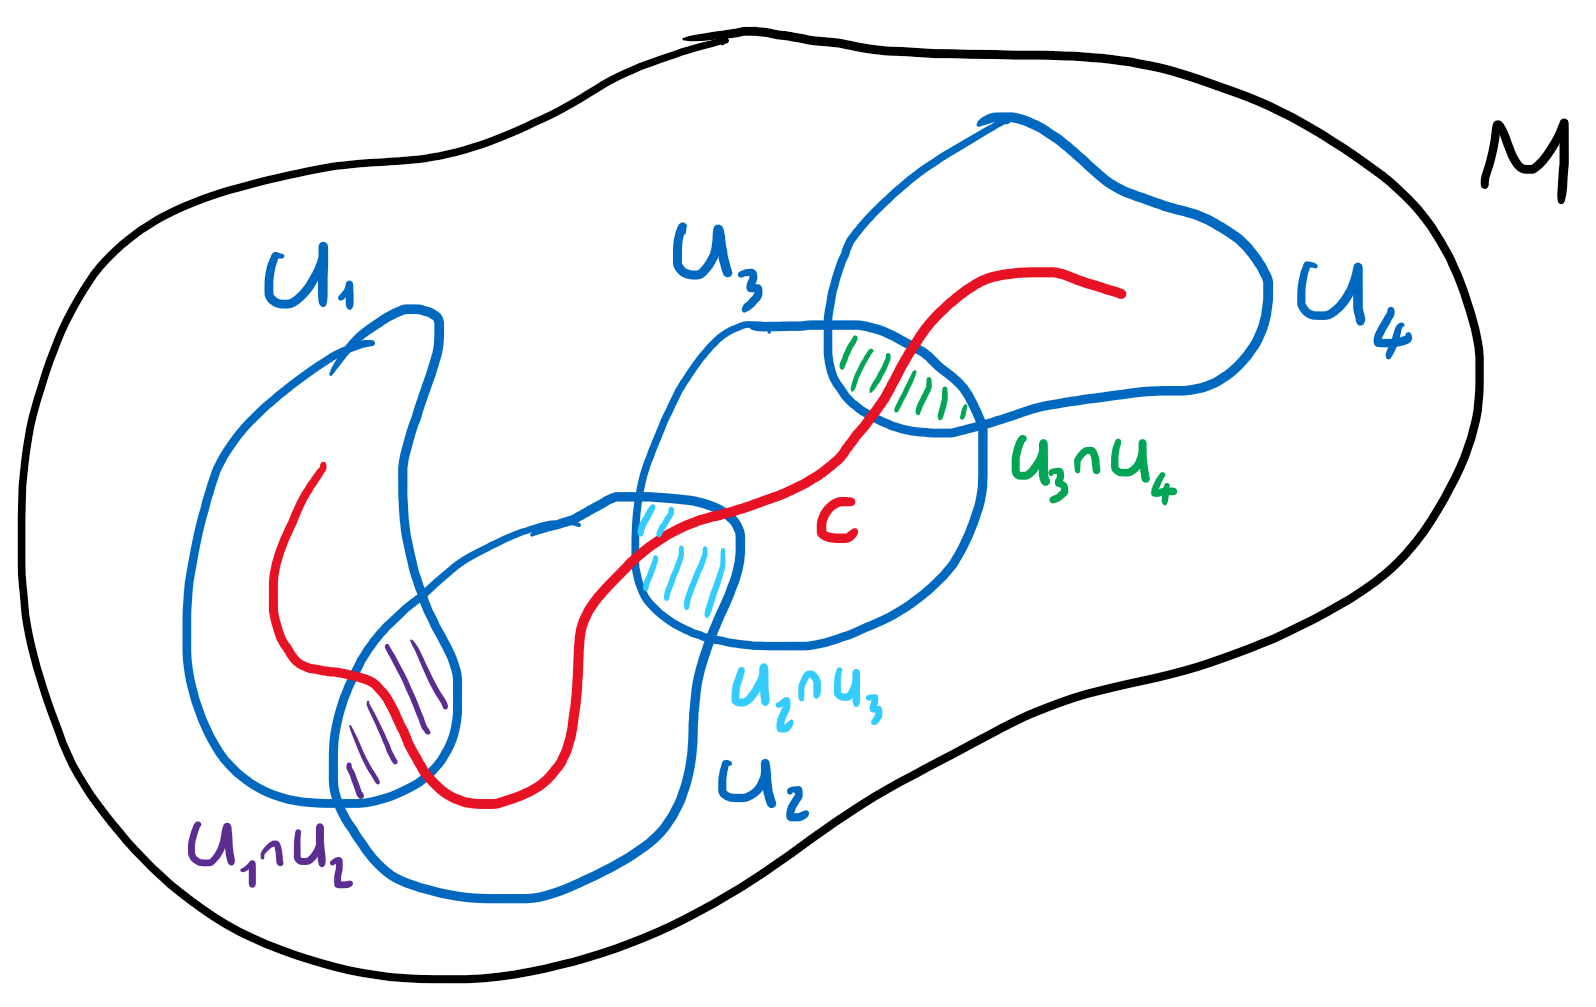
\includegraphics[width=0.6\textwidth,keepaspectratio]{img52}
\end{figure}

\begin{theorem}[Esistenza e unicità di curve integrali]
	Siano $ X \in \chi(M) $ e $ p \in M $, allora esiste ed è unica la curva integrale massimale $ c : (a(p),b(p)) \to M $ per il campo $ X $, i.e.
	
	\begin{equation}
		\begin{cases}
			c'(t) = X_{c(t)} & \forall t \in (a,b)\\
			c(0) = p
		\end{cases}
	\end{equation}
\end{theorem}

La curva integrale per un campo dipende dal punto $ p $ della varietà scelto: il seguente teorema asserisce che questa dipendenza è liscia

\begin{theorem}
	Siano un aperto $ V \in \R^{n} $ e una funzione liscia $ f : V \to \R^{n} $, allora per $ \forall p \in V $ esistono un intorno aperto $ W \subset V $ di $ p $, $ \varepsilon > 0 $ e una funzione liscia
	
	\begin{equation}
		F : (-\varepsilon,\varepsilon) \times W \to V
	\end{equation}

	tali che
	
	\begin{equation}
		\begin{cases}
			\dot{F}(t,q) = f(F(t,q)) & \forall (t,q) \in (-\varepsilon,\varepsilon) \times W\\
			F(0,q) = q
		\end{cases}
	\end{equation}

	dove il punto indica la derivata rispetto a $ t $.
\end{theorem}

Questo teorema può dunque essere trasposto sulle varietà:

\begin{theorem}\label{flux-var}
	Siano $ X \in \chi(M) $ e $ p \in M $, allora esiste un aperto $ W \subset M $ di $ p $, $ \varepsilon > 0 $ e una funzione liscia
	
	\begin{equation}
		F : (-\varepsilon,\varepsilon) \times W \to V
	\end{equation}

	tali che
	
	\begin{equation}
		\begin{cases}
			F'(t,q) = X_{F(t,q)} & \forall (t,q) \in (-\varepsilon,\varepsilon) \times W\\
			F(0,q) = q
		\end{cases}
	\end{equation}

	L'applicazione $ F(t,q) $ si chiama \textit{flusso locale del campo di vettori} $ X $.
\end{theorem}

Come notazione per i flussi, verrà utilizzato $ F_{t}(q) \doteq F(t,q) $.\\
La \textit{linea di flusso in} $ q $ è definita come $ F_{t}(q) $ al variare di $ t \in (-\varepsilon,\varepsilon) $ con $ q $ fissato: presa la curva integrale di $ X $ che inizia in $ q $ indicata come

\begin{equation}
	F(\cdot,q) : (-\varepsilon,\varepsilon) \to V
\end{equation}

la sua immagine è la linea di flusso. Questa curva integrale non è massimale per $ X $: il dominio non dipende dal punto ma è scelto perché la curva soddisfi la condizione per $ \forall q \in W $.\\
Se il flusso di $ X $ è \textit{globale}, i.e. definito in $ \R \times M $

\begin{equation}
	F : \R \times M \to M
\end{equation}

il campo di vettori $ X $ si dice \textit{completo}.

\begin{definition}
	Siano $ X \in \chi(M) $, $ F_{t}(q) $ il suo flusso locale e supponiamo che siano definiti $ F_{t} $, $ F_{s} $ e $ F_{t+s} $, allora
	
	\begin{equation}
		F_{t}(F_{s}(q)) = (F_{t} \circ F_{s})(q) = F_{t+s}(q)
	\end{equation}
\end{definition}

\begin{proof}
	Fissiamo il parametro $ s $ e il punto $ q $ e facciamo variare il parametro $ t $, per la definizione di flusso possiamo scrivere
	
	\begin{equation}
		\begin{cases}
			F'_{t}(F_{s}(q)) = X_{F_{t}(F_{s}(q))} & \forall t \in (-\varepsilon,\varepsilon)\\
			F_{0}(F_{s}(q)) = F(0,F_{s}(q)) = F_{s}(q)
		\end{cases}
	\end{equation}

	d'altra parte, ponendo $ u = t+s $
	
	\begin{equation}
		F'_{t+s}(q) = \dfrac{\operatorname{d}}{\operatorname{du}} F_{u}(q) = F'_{u}(q)
	\end{equation}

	dunque
	
	\begin{equation}
		\begin{cases}
			F'_{t+s}(q) = F'_{u}(q) = X_{F_{u}(q)} = X_{F_{t+s}(q)} & \forall t \in (-\varepsilon,\varepsilon)\\
			F_{0+s}(q) = F_{s}(q)
		\end{cases}
	\end{equation}

	siccome sia $ F_{t}(F_{s}(q)) $ che $ F_{t+s}(q) $ sono curve integrali per $ X $ e iniziano nello stesso punto $ F_{s}(q) $, per il teorema di unicità delle curve integrali
	
	\begin{equation}
		(F_{t} \circ F_{s})(q) = F_{t+s}(q)
	\end{equation}
\end{proof}

Nel caso in cui un campo di vettori $ X $ ammetta un flusso globale $ F : \R \times M \to M $, abbiamo che

\begin{equation}
	F_{t} \circ F_{s} = F_{t+s}, \qquad \forall t,s \in \R
\end{equation}

In particolare, se $ s = -t $ abbiamo che

\begin{equation}
	F_{t} \circ F_{-t} = F_{0} = \id_{M}
\end{equation}

i.e. $ F_{t} $ è invertibile con inversa $ (F_{t})^{-1} = F_{-t} $ e dunque $ F_{t} : M \to M $ è un diffeomorfismo per $ \forall t \in \R $: da questo è possibile ottenere un \textit{gruppo di diffeomorfismi a un parametro} tramite l'applicazione

\begin{align}
	\begin{split}
		G : \R &\to \operatorname{Diff}(M)\\
		t &\mapsto F_{t}
	\end{split}
\end{align}

\subsubsection{\textit{Esempi}}

\paragraph{1) Campo di vettori completo}

Sia il campo di vettori liscio $ X \in chi(\R^{2}) $ con la sua identificazione in $ \R^{2} $ definito come

\begin{equation}
	X = - y \dfrac{\partial}{\partial x} + x \dfrac{\partial}{\partial y} = (-y, x)
\end{equation}

L'obiettivo è trovare la curva integrale passante per un generico punto $ p = (p^{1},p^{2}) \in \R^{2} $ e il flusso di $ X $.\\
Sia $ c : (a,b) \to \R^{2} $ una curva integrale per $ X $ con

\begin{equation}
	\begin{cases}
		c(t) = (x(t),y(t))\\
		c(0) = p\\
		c'(t) = \dot{x}(t) \left. \dfrac{\partial}{\partial x} \right|_{c(t)} + \dot{y}(t) \left. \dfrac{\partial}{\partial y} \right|_{c(t)} = (\dot{x}(t),\dot{y}(t))		
	\end{cases}
\end{equation}

per trovare la forma della curva, eguagliamo il vettore tangente alla curva con il campo di vettori

\begin{align}
	\begin{split}
		c'(t) &= X_{c(t)}\\
		\dot{x}(t) \left. \dfrac{\partial}{\partial x} \right|_{c(t)} + \dot{y}(t) \left. \dfrac{\partial}{\partial y} \right|_{c(t)} &= - y(t) \left. \dfrac{\partial}{\partial x} \right|_{c(t)} + x(t) \left. \dfrac{\partial}{\partial y} \right|_{c(t)}
	\end{split}
\end{align}

da cui otteniamo il sistema di ODE

\begin{equation}
	\begin{cases}
		\dot{x}(t) = - y(t)\\
		\dot{y}(t) = x(t)\\
		x(0) = p^{1}\\
		y(0) = p^{2}
	\end{cases}
\end{equation}

derivando la prima equazione rispetto a $ t $ otteniamo

\begin{equation}
	\ddot{x}(t) = - \dot{y}(t) = - x(t) %
	\implies %
	\begin{cases}
		\ddot{x}(t) + x(t) = 0\\
		x(0) = p^{1}
	\end{cases}
\end{equation}

la cui soluzione è

\begin{equation}
	\begin{cases}
		x(t) = A \cos(t) + B \sin(t), \qquad A,B \in \R\\
		x(0) = p^{1} = A
	\end{cases}%
	\implies %
	x(t) = p^{1} \cos(t) + B \sin(t)
\end{equation}

per trovare l'altra soluzione

\begin{equation}
	\begin{cases}
		y(t) = - \dot{x}(t) = p^{1} \sin(t) - B \cos(t)\\
		y(0) = p^{2} = - B
	\end{cases}%
	\implies %
	y(t) = p^{1} \sin(t) + p^{2} \cos(t)
\end{equation}

dunque

\begin{equation}
	c(t) = (p^{1} \cos(t) - p^{2} \sin(t),p^{1} \sin(t) + p^{2} \cos(t))
\end{equation}

o alternativamente possiamo scrivere $ c(t) $ come vettore colonna

\begin{equation}
	c(t) = %
	\begin{bmatrix}
		x(t) \\\\ y(t)
	\end{bmatrix}%
	= %
	\begin{bmatrix}
		\cos(t) & - \sin(t) \\\\%
		\sin(t) & \cos(t)
	\end{bmatrix}%
	%
	\begin{bmatrix}
		p^{1} \\\\ p^{2}
	\end{bmatrix}
\end{equation}

Questo significa che le curve integrali, al variare del punto $ p $, sono cerchi concentrici di raggio $ \sqrt{(p^{1})^{2} + (p^{2})^{2}} $, i.e. la distanza del punto $ p $ dall'origine.\\
Il flusso del campo di vettori $ X $ è globale

\begin{align}
	\begin{split}
		F : \R \times \R^{2} &\to \R^{2}\\
		(t,q) = (t,q^{1},q^{2}) &\mapsto F_{t}(q) = %
		\begin{bmatrix}
			\cos(t) & - \sin(t) \\\\%
			\sin(t) & \cos(t)
		\end{bmatrix}%
		%
		\begin{bmatrix}
			q^{1} \\\\ q^{2}
		\end{bmatrix}
	\end{split}
\end{align}

dunque il campo $ X $ è completo.\\
Verifichiamo ora che valga la legge di composizione dei flussi:

\begin{align}
	\begin{split}
		F_{t+s} &= F_{t} \circ F_{s}\\\\
		%
		\begin{bmatrix}
			\cos(t+s) & - \sin(t+s) \\\\%
			\sin(t+s) & \cos(t+s)
		\end{bmatrix}%
		&= %
		\begin{bmatrix}
			\cos(t) & - \sin(t) \\\\%
			\sin(t) & \cos(t)
		\end{bmatrix}%
		\begin{bmatrix}
			\cos(s) & - \sin(s) \\\\%
			\sin(s) & \cos(s)
		\end{bmatrix}
	\end{split}
\end{align}

questo è vero in quanto le due matrici rappresentano rotazioni rispettivamente di angoli $ t $ ed $ s $ e queste rispettano la stessa legge di composizione dei flussi.

\paragraph{2) Campo di vettori non completo}

Sia il campo di vettori liscio $ X \in chi(\R \setminus \{0\}) $

\begin{equation}
	X = x^{2} \dfrac{\partial}{\partial x}
\end{equation}

L'obiettivo è trovare la curva integrale passante per un generico punto $ p \in \R \setminus \{0\} $ e il flusso di $ X $.\\
Sia $ c : (a,b) \to \R \setminus \{0\} $ una curva integrale per $ X $, chiamando $ c(t) = x(t) $, abbiamo che

\begin{equation}
	\begin{cases}
		\dot{x}(t) = x^{2}(t)\\
		x(0) = p
	\end{cases}
\end{equation}

risolvendo la ODE

\begin{equation}
	\dfrac{\operatorname{dx}}{\operatorname{dt}} = x^{2} %
	\implies %
	\dfrac{\operatorname{dx}}{x^{2}} = \operatorname{dt} %
	\implies %
	- \dfrac{1}{x} = t + c, \quad c \in \R
\end{equation}

da cui

\begin{equation}
	\begin{cases}
		x(t) = - \dfrac{1}{t + c}\\\\
		x(0) = p = - \dfrac{1}{c}
	\end{cases}%
	\implies %
	c = - \dfrac{1}{p} %
	\implies %
	x(t) = - \dfrac{1}{t - \dfrac{1}{p}}
\end{equation}

la soluzione è dunque la curva integrale

\begin{equation}
	x(t) = \dfrac{p}{1 - t p}
\end{equation}

Sappiamo, dal teorema, che esiste un intervallo massimale su cui è definita (che deve contenere 0): è necessario che $ 1-tp \neq 0 $ perciò

\begin{equation}
	\begin{cases}
		c : \left( -\infty, \dfrac{1}{p} \right) \to \R \setminus \{0\} & p > 0\\\\
		c : \left( -\dfrac{1}{p}, \infty \right) \to \R \setminus \{0\} & p < 0
	\end{cases}
\end{equation}

siccome non è possibile estendere il dominio a tutto $ \R $, il campo di vettori $ X $ non è completo.\\
Considerando $ p>0 $, i.e. $ t \in (-\infty, \sfrac{1}{p}) $, e $ q \in \R \setminus \{0\} $, otteniamo il flusso locale

\begin{align}
	\begin{split}
		F : \left( -\infty, \dfrac{1}{p} \right) \times \R \setminus \{0\} &\to \R \setminus \{0\}\\
		(t,q) &\mapsto \dfrac{q}{1 - t q}
	\end{split}
\end{align}

Verifichiamo ora che valga la legge di composizione dei flussi:

\begin{align}
	\begin{split}
		(F_{t} \circ F_{s})(q) &= F_{t} \left( \dfrac{q}{1 - s q} \right)\\\\
		&= \dfrac{\dfrac{q}{1 - s q}}{1 - t \left( \dfrac{q}{1 - s q} \right)}\\\\
		&= \dfrac{q}{(1 - s q) \left(1 - \dfrac{t q}{1 - s q} \right)}\\\\
		&= \dfrac{q}{1 - s q - t q}\\\\
		&= \dfrac{q}{1 - (t+s) q}\\\\
		&= F_{t+s}(q)
	\end{split}
\end{align}

supponendo che $ t+s $ sia definito.

\subsection{Commutatore tra due campi di vettori}

Consideriamo le identificazioni tra i campi di vettori e le derivazioni $ \chi(M) = Der(C^{\infty}(M)) $ e tra una funzione liscia e la sua derivata tramite un campo di vettori

\begin{equation}
	f \in C^{\infty}(M) \to X f \in C^{\infty}(M)
\end{equation}

Presi $ X,Y \in \chi(M) = Der(C^{\infty}(M)) $, l'applicazione liscia

\begin{align}
	\begin{split}
		X Y : C^{\infty}(M) &\to C^{\infty}(M)\\
		f &\mapsto X(Y(f))
	\end{split}
\end{align}

è $ \R $-lineare

\begin{align}
	\begin{split}
		X Y (\lambda f + \mu g) &= X (\lambda Y f + \mu Y g)\\
		&= \lambda (XY)(f) + \mu (XY)(g)
	\end{split}
\end{align}

ma $ XY \notin Der(C^{\infty}(M)) $, i.e. non rispetta la regola di Leibniz

\begin{align}
	\begin{split}
		(XY)(fg) &= X ((Yf) g + f (Y g))\\
		&= X(Y(f)) \, g + Y(f) \, X(g) + X(f) \, Y(g) + f \, X(Y(g))\\
		&\neq X(Y(f)) \, g + f \, X(Y(g))
	\end{split}
\end{align}

Definiamo quindi il \textit{commutatore o "bracket" tra due campi di vettori} come\footnote{%
	Alternativamente si può scrivere
%	rifai questa applicazione con \maps{}{}{}{}{}
	\begin{align}
		\begin{split}
			[\cdot,\cdot] : Der(C^{\infty}(M)) \times Der(C^{\infty}(M)) &\to Der(C^{\infty}(M))\\
			(X,Y) &\mapsto XY-YX
		\end{split}
	\end{align}%
}

\begin{align}
	\begin{split}
		[\cdot,\cdot] : \chi(M) \times \chi(M) &\to \chi(M)\\
		(X,Y) &\mapsto XY-YX
	\end{split}
\end{align}

e dunque, siccome questo rispetta anche la regola di Leibniz

\begin{equation}
	[X,Y] = XY-YX \in Der(C^{\infty}(M))
\end{equation}

Di seguito, la verifica:

\begin{align}
	\begin{split}
		[X,Y](fg) &= (XY-YX)(fg)\\
		&= (XY)(fg) - (YX)(fg)\\
		&= ( \, X((Yf) g + f (Y g)) \, ) - ( \, Y((Xf) g + f (X g)) \, )\\
		&= ( \, X(Y(f)) \, g + Y(f) \, X(g) + X(f) \, Y(g) + f \, X(Y(g)) \, ) + \\
		& \hal - ( \, Y(X(f)) \, g + X(f) \, Y(g) + Y(f) \, X(g) + f \, Y(X(g)) \, )\\
		%
		&= X(Y(f)) \, g + Y(f) \, X(g) + X(f) \, Y(g) + f \, X(Y(g)) + \\
		& \hal - Y(X(f)) \, g - X(f) \, Y(g) - Y(f) \, X(g) - f \, Y(X(g))\\
		%
		&= X(Y(f)) \, g - Y(X(f)) \, g + f \, X(Y(g)) - f \, Y(X(g))\\
		&= (XY-YX)(f) \, g + f \, (XY-YX)(g)\\
		&= [X,Y](f) \, g + f \, [X,Y](g)
	\end{split}
\end{align}

A questo punto, considerati un aperto $ U $, un suo punto $ p \in U $, due campi di vettori lisci $ X,Y \in \chi(U) $ e una funzione liscia $ f \in C^{\infty}(U) $, possiamo definire il commutatore dei due campi come

\begin{equation}
	[X,Y]_{p}(f) = X_{p} (Y(f))
\end{equation}

dove $ Y(f) \in C^{\infty}(U) $ e $ [X,Y] \in \chi(U) $ in quanto questo è $ \R $-lineare

\begin{equation}
	[X,Y]_{p}(\lambda f + \mu g) = \lambda [X,Y]_{p}(f) + \mu [X,Y]_{p}(g)
\end{equation}

perché lo è $ X_{p} $, rispetta la regola di Leibniz

\begin{align}
	\begin{split}
		[X,Y]_{p}(fg) &= [X,Y](fg)(p)\\
		&= ([X,Y](f) \, g + f \, [X,Y](g))(p)\\
		&= [X,Y]_{p}(f) \, g(p) + f(p) \, [X,Y]_{p}(g)
	\end{split}
\end{align}

perché la rispetta $ [X,Y] \in Der(C^{\infty}(U)) $ ed è effettivamente un campo di vettori liscio in quanto è liscia la composizione $ XY-YX $, i.e.

\begin{align}
	\begin{split}
		[X,Y]_{p}(f) &= [X,Y](f)(p)\\
		&= (XY-YX)(f)(p) \in C^{\infty}(U)\\
	\end{split}
\end{align}

\begin{definition}
	Siano una varietà differenziabile $ M $ di dimensione $ n $, due campi di vettori lisci $ X,Y \in \chi(M) $ e due funzioni lisce $ f,g \in C^{\infty}(M) $:
	
	\begin{itemize}
		\item Vale la proprietà
		
		\begin{equation}
			[f X, g Y] = f g [X,Y] + (f \, X(g)) \, Y - (g \, Y(f)) \, X
		\end{equation}
	
		dove $ (f \, X(g)), (g \, Y(f)) \in C^{\infty}(M) $;
	
		\item Presa una carta $ (U,\phi) \in M $ con $ \phi = (x^{1},\dots,x^{n}) $, e le forme locali dei campi tramite la carta
		
		\begin{align}
			\begin{split}
				X_{|U} &= \sum_{j=1}^{n} a^{j} \dfrac{\partial}{\partial x^{j}}\\
				Y_{|U} &= \sum_{j=1}^{n} b^{j} \dfrac{\partial}{\partial x^{j}}
			\end{split}
		\end{align}
	
		con $ a^{j},b^{j} \in C^{\infty}(U) $ per $ \forall j=1,\dots,n $, abbiamo che la forma locale del commutatore tra i campi è la seguente
		
		\begin{equation}
			[X,Y]_{|U} = \sum_{j,k=1}^{n} \left( a^{j} \dfrac{\partial b^{k}}{\partial x^{j}} + b^{j} \dfrac{\partial a^{k}}{\partial x^{j}} \right) \dfrac{\partial}{\partial x^{k}}
		\end{equation}
	\end{itemize}
\end{definition}

\begin{proof}
	Per la prima proprietà:
	
	\begin{align}
		\begin{split}
			[f X, g Y](h) &= f X(g \, Y(h)) - g Y(f \, X(h))\\
			&= f ( \, X(g) \, Y(h) + g \, XY(h) \, ) + \\
			& \hal - g ( \, Y(f) \, X(h) + f \, YX(h) \, )\\
			%
			&= f \, X(g) \, Y(h) + f g \, XY(h) + \\
			& \hal - g \, Y(f) \, X(h) - g f \, YX(h)\\
			%
			&= f g (XY-YX)(h) + f \, X(g) \, Y(h) - g \, Y(f) \, X(h)\\
			&= ( \, f g [X,Y] + (f \, X(g)) \, Y - (g \, Y(f)) \, X \, )(h)
		\end{split}
	\end{align}

	in quanto $ fg \equiv gf $.\\
	Per al seconda, usando la proprietà dimostrata sopra:
	
	\begin{align}
		\begin{split}
			[X,Y]_{|U} &= \left[ \sum_{j=1}^{n} a^{j} \dfrac{\partial}{\partial x^{j}} , \sum_{k=1}^{n} b^{k} \dfrac{\partial}{\partial x^{k}} \right]\\
			&= \sum_{j,k=1}^{n} a^{j} b^{k} \cancel{\left[ \dfrac{\partial}{\partial x^{j}} , \dfrac{\partial}{\partial x^{k}} \right]} + \\
			& \hal + \sum_{j,k=1}^{n} a^{j} \dfrac{\partial b^{k}}{\partial x^{j}} \dfrac{\partial}{\partial x^{k}} - \sum_{j,k=1}^{n} b^{k} \dfrac{\partial a^{j}}{\partial x^{k}} \dfrac{\partial}{\partial x^{j}}\\
			&= \sum_{j,k=1}^{n} a^{j} \dfrac{\partial b^{k}}{\partial x^{j}} \dfrac{\partial}{\partial x^{k}} - \sum_{j,k=1}^{n} b^{j} \dfrac{\partial a^{k}}{\partial x^{j}} \dfrac{\partial}{\partial x^{k}}\\
			&= \sum_{j,k=1}^{n} \left( a^{j} \dfrac{\partial b^{k}}{\partial x^{j}} + b^{j} \dfrac{\partial a^{k}}{\partial x^{j}} \right) \dfrac{\partial}{\partial x^{k}}
		\end{split}
	\end{align}

	dove il commutatore nel secondo passaggio è nullo in quanto le derivate parziali (applicate a una qualsiasi funzione) commutano e, sempre nello stesso passaggio, nell'ultima sommatoria possiamo scambiare gli indici $ j $ e $ k $ in quanto muti.
\end{proof}

\subsection{Distribuzioni e teorema di Frobenius}

Sia $ M $ una varietà differenziabile di dimensione $ n $, una \textit{distribuzione} $ r $\textit{-dimensionale} ($ r \leqslant n $) è un'assegnazione $ \forall p \in M $ di un sottospazio $ D_{p} \subseteq T_{p}(M) $ tale che $ \dim(D_{p}) = r $; una distribuzione è, in sostanza, una famiglia di sottospazi dello spazio tangente punto per punto. Una distribuzione $ r $-dimensionale è liscia se per $ \forall p \in M $ esistono un intorno aperto $ U \subset M $ di $ p $ e un'insieme di $ r $ campi di vettori lisci $ X_{1},\dots,X_{r} \in \chi(M) $ tali che

\begin{equation}
	D_{p} = \left\langle (X_{1})_{p}, \dots, (X_{r})_{p} \right\rangle_{\R}
\end{equation}

Una distribuzione è liscia perché varia in tale modo rispetto al punto a cui è legata.\\
Sia $ D $ una distribuzione liscia $ r $-dimensionale, una \textit{varietà integrale} di $ D $ è una varietà differenziabile $ S \subset M $ (non necessariamente una sottovarietà) tale che

\begin{equation}
	T_{p}(S) = D_{p}, \qquad \forall p \in M
\end{equation}

con $ \dim(S) = r $, cioè che ha, in ogni suo punto, come spazio tangente una distribuzione liscia.\\
Una distribuzione liscia $ r $-dimensionale $ D $ è \textit{completamente integrabile} se per $ \forall q \in M $ esiste una varietà integrale $ S $ per $ D $ tale che $ q \in S $, cioè se esiste una varietà integrabile per ogni punto della varietà.\\\\
%
Ad esempio, sia un campo di vettori $ X \in \chi(M) $ non nullo in un aperto $ U $, i.e. $ X \neq 0 $ in $ U \subset M $ e consideriamo la distribuzione liscia 1-dimensionale

\begin{equation}
	D = \{ \lambda X \mid \lambda \in \R \} %
	\implies%
	D_{p} = \{ \lambda X_{p} \mid \lambda \in \R \}
\end{equation}

ciò significa che, per ogni punto, la distribuzione individua la retta nella direzione del vettore $ X_{p} $.\\
Questa distribuzione è completamente integrabile in quanto per $ \forall q \in M $ esiste la curva integrale di $ X $ che passa per $ q $: questo significa che la curva integrale è anche una varietà integrale.\\\\
%
Data una distribuzione $ D $, un campo di vettori $ X \in \chi(M) $ appartiene alla distribuzione se $ X_{p} \in D_{p} $ per $ \forall p \in M $. Nella distribuzione dell'esempio precedente $ f X \in D $ per $ \forall f \in C^{\infty}(M) $ con $ f \neq 0 $.

\begin{theorem}[Frobenius]
	Sia $ D $ una distribuzione $ r $-dimensionale liscia su una varietà differenziabile $ M $, allora $ D $ è completamente integrabile se e solo se $ D $ è involutoria, i.e.
	
	\begin{equation}
		\begin{cases}
			D \text{ involutoria}\\
			X,Y \in D
		\end{cases}
		\implies%
		[X,Y] \in D
	\end{equation}
\end{theorem}

\begin{remark}
	Il teorema di Frobenius implica il teorema di esistenza di curve integrali per un campo di vettori.
\end{remark}

Se $ X_{p} = 0 $ allora la curva integrale per $ X $ che inizia in $ p $ è costante\footnote{%
	Vedi Esercizio \ref{es2-32}.%
}. A questo punto, supponiamo che $ X_{p} \neq 0 $ e consideriamo un intorno $ U $ di $ p $ dove $ X_{q} \neq 0 $ per $ \forall q \in U $ e la distribuzione liscia 1-dimensionale

\begin{equation}
	D = \{ \lambda X \mid \lambda \in \R \}
\end{equation}

dove $ D_{p} = \langle X_{p} \rangle_{\R} $. L'esistenza di una curva integrale che passa per $ p $ è verificata se $ D $ è involutoria, i.e. (per il teorema di Frobenius) $ D $ è completamente integrabile e quindi esiste la curva integrale ricercata.\\
Per dimostrare che $ D $ sia involutoria è necessario che, presi due campi di vettori della distribuzione $ Y,Z \in D $, il commutatore di questi appartiene ancora alla distribuzione, i.e. $ [Y,Z] \in D $: per la distribuzione considerata in precedenza

\begin{equation}
	Y,Z \in D \iff Y = fX \wedge Z = gX \quad f,g \in C^{\infty}(U)
\end{equation}

in quanto la moltiplicazione di un campo di vettori liscio per una funzione liscia è ancora un vettore liscio (nella stessa direzione), calcolando ora il commutatore tra i due campi

\begin{align}
	\begin{split}
		[Y,Z] &= [fX,gX]\\
		&= fg [X,X] + (f \, X(g)) X - (g \, X(f)) X\\
		&= (f \, X(g) - g \, X(f)) X \in D
	\end{split}
\end{align}

Questo implica dunque l'esistenza di una curva integrale passante per $ p $.

\subsubsection{\textit{Esempio}}

\paragraph{Distribuzione non integrabile}

Prendiamo $ \R^{3} $ e i campi di vettori lisci (con la loro identificazione)

\begin{equation}
	\begin{cases}
		X = z \dfrac{\partial}{\partial x} + \dfrac{\partial}{\partial z} = (z,0,1)\\\\
		Y = \dfrac{\partial}{\partial y} + \dfrac{\partial}{\partial z} = (0,1,1)
	\end{cases}
\end{equation}

Consideriamo la distribuzione liscia 2-dimensionale

\begin{equation}
	D = \{ \lambda X + \mu Y \mid \lambda,\mu \in \R \}
\end{equation}

Se $ D $ fosse completamente integrabile, per ogni punto di $ \R^{3} $ esisterebbe una superficie il cui spazio tangente è generato da una combinazione lineare dei campi di vettori (definiti sopra) valutati in quello stesso punto.\\
Verifichiamo ora che non sia completamente integrabile: per farlo, è sufficiente esibire un controesempio, i.e. un commutatore tra i campi della distribuzione che non sia appartenente alla distribuzione, prendiamo dunque semplicemente il commutatore tra i campi $ X $ e $ Y $

\begin{align}
	\begin{split}
		[X,Y] &= \left[ z \dfrac{\partial}{\partial x} + \dfrac{\partial}{\partial z} , \dfrac{\partial}{\partial y} + \dfrac{\partial}{\partial z} \right]\\
		&= \left[ z \dfrac{\partial}{\partial x}, \dfrac{\partial}{\partial y} \right] + \left[ z \dfrac{\partial}{\partial x}, \dfrac{\partial}{\partial z} \right] + \cancel{\left[ \dfrac{\partial}{\partial z}, \dfrac{\partial}{\partial y} \right]} + \cancel{\left[ \dfrac{\partial}{\partial z}, \dfrac{\partial}{\partial z} \right]}\\
		&= \left[ z \dfrac{\partial}{\partial x}, \dfrac{\partial}{\partial y} \right] + \left[ z \dfrac{\partial}{\partial x}, \dfrac{\partial}{\partial z} \right]\\
		&= (z \cdot 1) \cancel{\left[ \dfrac{\partial}{\partial x}, \dfrac{\partial}{\partial y} \right]} + \left( z \, \cancel{\dfrac{\partial 1}{\partial x}} \right) \dfrac{\partial}{\partial y} - \cancel{\left( \dfrac{\partial z}{\partial y} \right)} \dfrac{\partial}{\partial x} + \\
		& \hal + (z \cdot 1) \cancel{\left[ \dfrac{\partial}{\partial x}, \dfrac{\partial}{\partial z} \right]} + \left( z \, \cancel{\dfrac{\partial 1}{\partial x}} \right) \dfrac{\partial}{\partial z} - \cancelto{1}{\left( \dfrac{\partial z}{\partial z} \right)} \dfrac{\partial}{\partial x}\\
		%
		&= - \dfrac{\partial}{\partial x} \notin D
	\end{split}
\end{align}

Questo prova che $ D $ non è involutoria e quindi, per il teorema di Frobenius, non è completamente integrabile.

\paragraph{4. Campi di vettori}

Siano $ M $ una varietà differenziabile, $ \chi(M) $ l'insieme dei campi di vettori lisci sulla varietà e il commutatore

\begin{equation}
	[X,Y] = XY - YX, \qquad X,Y \in \chi(M)
\end{equation}

allora $ (\chi(M),[,]) $ è un'algebra di Lie su $ \R $. Lo spazio vettoriale $ \chi(M) $ ha dimensione infinita.

\section{Pushforward di campi di vettori}

Siano $ N $ e $ M $ due varietà differenziabili di dimensione rispettivamente $ n $ ed $ m $, un'applicazione liscia $ F : N \to M $ e un campo di vettori liscio $ X \in \chi(M) $. Fissando un punto $ p \in N $, per associare un vettore del campo dallo spazio tangente di $ N $ in $ p $ a quello di $ M $ in $ F(p) $ possiamo usare il differenziale

\map{F_{*p}}
	{T_{p}(N)}{T_{F(p)}(M)}
	{X_{p}}{F_{*p}(X_{p})}

ma questo non può essere esteso a tutto il campo di vettori in quanto, se l'applicazione non fosse iniettiva, esisterebbero $ p,q \in N $ tali che $ F(p) = F(q) $: a questo punto si presenta l'assegnazione del vettore in $ F(p) = F(q) $ e ci sarebbe ambiguità tra $ F_{*p}(X_{p}) $ e $ F_{*p}(X_{q}) $ e tra $ F_{*q}(X_{p}) $ e $ F_{*q}(X_{q}) $. Anche se fosse iniettiva ma comunque non suriettiva, non esisterebbe un vettore $ X_{p} \in \chi(N) $ in $ p \in N $ la cui immagine attraverso il differenziale $ F_{*p} $ sia un vettore in un punto $ r \in M \setminus F(N) $ (dove $ F(N) \subsetneqq M $ in quanto $ F $ non è suriettiva).\\\\
%
Supponiamo ora che l'applicazione $ F : N \to M $ sia un diffeomorfismo (quindi sia iniettiva che suriettiva) e definiamo

\begin{equation}
	(F_{*} (X))_{q} = F_{*F^{-1}(q)} (X_{F^{-1}(q)})
\end{equation}

per $ \forall q \in N $ e $ (F_{*} (X))_{q} \in T_{q}(M) $; la definizione utilizza $ F^{-1}(q) $ in quanto $ F $ è biettiva e dunque $ F^{-1}(q) $ è l'unico punto che viene mandato in $ q $ tramite $ F $.

\begin{definition}
	$ F_{*}(X) $, chiamato \textit{pushforward di} $ X $ tramite il diffeomorfismo $ F $, è un campo di vettori liscio su $ M $, i.e. $ F_{*}(X) \in \chi(M) $.
\end{definition}

\begin{proof}
	Siccome $ (F_{*} (X))_{q} \in T_{q}(M) $ per $ \forall q \in N $, dobbiamo solo dimostrare che $ F_{*}(X) $ sia liscio, i.e.
	
	\begin{equation}
		(F_{*}(X))(g) \in C^{\infty}(M), \qquad g \in C^{\infty}(M)
	\end{equation}

	Prendendo $ q \in M $
	
	\begin{align}
		\begin{split}
			(F_{*}(X))(g)(q) &= (F_{*}(X))_{q}(g)\\
			&\doteq F_{*F^{-1}(q)} (X_{F^{-1}(q)})(g)\\
			&\doteq X_{F^{-1}(q)} (g \circ F)\\
			&= X (g \circ F)(F^{-1}(q))\\
			&= ((X (g \circ F)) \circ F^{-1})(g)
		\end{split}
	\end{align}

	dove nel secondo passaggio abbiamo usato la definizione di pushforward e nel terzo quella di differenziale; a questo punto $ (X (g \circ F)) \circ F^{-1} \in C^{\infty}(M) $ in quanto composizione di funzioni lisce.
\end{proof}

\subsection{Campi di vettori $ F $-related}

Siano $ F : N \to M $ una funzione liscia (non necessariamente un diffeomorfismo) e due campi di vettori lisci $ X \in \chi(N) $ e $ Y \in \chi(M) $, si dice che $ X $ è $ F $\textit{-related a} $ Y $ se

\begin{equation}
	F_{*p}(X_{p}) = Y_{F(p)}, \qquad p \in N
\end{equation}

\begin{remark}
	Se $ F $ è un diffeomorfismo, allora $ X $ è $ F $-related a $ Y $ se e solo se $ Y $ è il pushforward di $ X $, i.e. $ Y = F_{*}(X) $.
\end{remark}

\begin{proof}
	\begin{equation}
		Y_{F(p)} = F_{*p}(X_{p}) = (F_{*}(X))_{F(p)}, \quad \forall p \in N %
		\implies%
		Y = F_{*}(X)
	\end{equation}
\end{proof}

\begin{theorem}
	Siano $ F : N \to M $ una funzione liscia e due campi di vettori lisci $ X \in \chi(N) $ e $ Y \in \chi(M) $, allora $ X $ è $ F $-related a $ Y $ se e solo se
	
	\begin{equation}
		X(g \circ F) = (Y g) \circ F, \qquad \forall g \in C^{\infty}(M)
	\end{equation}

	con $ g : M \to \R $ e quindi $ g \circ F \in C^{\infty}(N) $.
\end{theorem}

\begin{proof}
	Per definizione, $ X $ è $ F $-related a $ Y $ se e solo se
	
	\begin{equation}
		F_{*p}(X_{p}) = Y_{F(p)}, \qquad p \in N
	\end{equation}

	applicando la definizione a una funzione qualsiasi $ g \in C^{\infty}(M) $ e usando la definizione di differenziale, deve valere
	
	\begin{align}
		\begin{split}
			(F_{*p}(X_{p}))(g) &= Y_{F(p)}(g)\\
			X_{p}(g \circ F) &= (Y g)(F(p))\\
			X(g \circ F)(p) &= ((Y g) \circ F)(p)\\
			X(g \circ F) = (Y g) \circ F
		\end{split}
	\end{align}
\end{proof}

\begin{theorem}
	Siano $ F : N \to M $ una funzione liscia e i campi di vettori lisci $ X_{1},X_{2} \in \chi(N) $ e $ Y_{1},Y_{2} \in \chi(M) $ con $ X_{1} $ $ F $-related a $ Y_{1} $ e $ X_{2} $ $ F $-related a $ Y_{2} $, i.e.
	
	\begin{equation}
		\begin{cases}
			Y_{1} = F_{*}(X_{1})\\
			Y_{2} = F_{*}(X_{2})
		\end{cases}
	\end{equation}

	allora il commutatore $ [X_{1},X_{2}] $ è $ F $-related a $ [Y_{1},Y_{2}] $.
\end{theorem}

Questo teorema asserisce che il commutatore tra due campi viene preservato tramite campi $ F $-related.

\begin{proof}
	Usando il teorema precedente, $ [X_{1},X_{2}] $ è $ F $-related a $ [Y_{1},Y_{2}] $ se e solo se
	
	\begin{equation}
		[X_{1},X_{2}](g \circ F) = ([Y_{1},Y_{2}] g) \circ F, \qquad \forall g \in C^{\infty}(M)
	\end{equation}

	Sempre usando il teorema precedente
	
	\begin{align}
		\begin{split}
			[X_{1},X_{2}](g \circ F) &= (X_{1} X_{2} - X_{2} X_{1})(g \circ F)\\
			&= (X_{1} X_{2})(g \circ F) - (X_{2} X_{1})(g \circ F)\\
			&= X_{1}((Y_{2} g) \circ F) - X_{2}((Y_{1} g) \circ F)\\
			&= Y_{1}(Y_{2} g) \circ F - Y_{1}(Y_{2} g) \circ F\\
			&= (Y_{1} Y_{2} - Y_{1} Y_{2})(g \circ F)\\
			&= [Y_{1},Y_{2}](g \circ F)
		\end{split}
	\end{align}
\end{proof}

\begin{corollary}\label{frel-brack}
	Siano $ F : N \to M $ un diffeomorfismo e i campi di vettori lisci $ X_{1},X_{2} \in \chi(N) $, allora il pushforward del commutatore è uguale al commutatore dei pushforward, i.e.
	
	\begin{equation}
		F_{*} ([X_{1},X_{2}]) = [F_{*} (X_{1}),F_{*} (X_{2})]
	\end{equation}

	Il pushforward commuta dunque con il commutatore.
\end{corollary}

\begin{proof}
	Per l'osservazione precedente, $ X_{i} $ è $ F $-related a $ F_{*}(X_{i}) $ per $ i=1,2 $ (poiché $ F $ è un diffeomorfismo). Per il teorema precedente $ [X_{1},X_{2}] $ è $ F $-related a $ [F_{*} (X_{1}),F_{*} (X_{2})] $ e ancora per l'osservazione precedente
	
	\begin{equation}
		F_{*} ([X_{1},X_{2}]) = [F_{*} (X_{1}),F_{*} (X_{2})]
	\end{equation}
\end{proof}